% !TeX spellcheck = en_US, gr_GR

\newglossaryentry{uncertainty}
{name={\foreignlanguage{greek}{αβεβαιότητα}},
	description={\foreignlanguage{greek}{Στο πλαίσιο της} \glsentryuserii{ml},\index{\foreignlanguage{greek}{αβεβαιότητα}} 
		\foreignlanguage{greek}{η αβεβαιότητα αναφέρεται στην παρουσία πολλαπλών εύλογων αποτελεσμάτων ή}
		\glsentryuserv{explanation} \foreignlanguage{greek}{με βάση τα διαθέσιμα} \glsentryuseriii{data}. 
		\foreignlanguage{greek}{Για παράδειγμα, η} \glsentryuseri{prediction} $\hat{\hypothesis}(\featurevec)$ 
		\foreignlanguage{greek}{που παράγεται από ένα εκπαιδευμένο} \glsentryuseriii{model} \glsentryuserii{ml} $\hat{\hypothesis}$
	 	\foreignlanguage{greek}{συχνά αντανακλά ένα πεδίο πιθανών τιμών για την αληθή} \glsentryuseriii{label} 
		\foreignlanguage{greek}{ενός συγκεκριμένου} \glsentryuserii{datapoint}. \foreignlanguage{greek}{Όσο πιο ευρύ το 
		πεδίο, τόσο μεγαλύτερη η σχετική αβεβαιότητα. Η θεωρία} \glsentryuserv{probability} \foreignlanguage{greek}{μας 
		επιτρέπει να αναπαριστούμε, να ποσοτικοποιούμε, και να συλλογιστούμε για την αβεβαιότητα με έναν 
		μαθηματικά ενδελεχή τρόπο.} \\
		\foreignlanguage{greek}{Βλέπε επίσης:} \gls{ml}, \gls{explanation}, \gls{data}, \gls{prediction}, \gls{model}, \gls{label}, 
		\gls{datapoint}, \gls{probability}, \gls{probmodel}, \gls{risk}, \gls{entropy}, \gls{variance}.},
	first={\foreignlanguage{greek}{αβεβαιότητα}},
	text={\foreignlanguage{greek}{αβεβαιότητα}},
	user1={\foreignlanguage{greek}{αβεβαιότητα}}, %nominative
  	user2={\foreignlanguage{greek}{αβεβαιότητας}}, %genitive
	user3={\foreignlanguage{greek}{αβεβαιότητα}} %accusative
}

\newglossaryentry{optimism in the face of uncertainty}
{name={\foreignlanguage{greek}{αισιοδοξία παρά την αβεβαιότητα}},
	description={\foreignlanguage{greek}{Οι μέθοδοι} \glsentryuserii{ml}\index{\foreignlanguage{greek}{αισιοδοξία παρά την αβεβαιότητα}} 
		\foreignlanguage{greek}{μαθαίνουν} \glsentryuseriii{modelparams} $\weights$ 
		\foreignlanguage{greek}{σύμφωνα με κάποιο κριτήριο επίδοσης $\bar{f}(\weights)$. Ωστόσο, δεν μπορούν να έχουν άμεση 
		πρόσβαση στο $\bar{f}(\weights)$, αλλά βασίζονται σε μία εκτίμηση (ή προσέγγιση) 
		$f(\weights)$ του $\bar{f}(\weights)$. Ως ένα χαρακτηριστικό παράδειγμα, οι μέθοδοι βασιμένες στην} \glsentryuseriii{erm}  
		\foreignlanguage{greek}{χρησιμοποιούν τη μέση} \glsentryuseriii{loss} \foreignlanguage{greek}{σε ένα συγκεκριμένο} \glsentryuseriii{dataset} 
		\foreignlanguage{greek}{(δηλαδή το} \glsentryuseriii{trainset}) \foreignlanguage{greek}{ως μία εκτίμηση για τη}  
		\glsentryuseriii{risk} \foreignlanguage{greek}{μίας} \glsentryuserii{hypothesis}. \foreignlanguage{greek}{Χρησιμοποιώντας ένα} 
		\glsentryuseriii{probmodel}, \foreignlanguage{greek}{μπορεί κανείς να κατασκευάσει ένα διάστημα εμπιστοσύνης  
		$\big[ l^{(\weights)},  u^{(\weights)} \big]$ για κάθε επιλογή $\weights$ για τις} \glsentryuseriii{modelparams}.
		\foreignlanguage{greek}{Μία απλή κατασκευή είναι $l^{(\weights)} \defeq f(\weights) - \sigma/2$, $u^{(\weights)} \defeq f(\weights)+ \sigma/2$, 
	    	με το $\sigma$ να είναι ένα μέτρο της (αναμενόμενης) απόκλισης του $f(\weights)$ από το $\bar{f}(\weights)$.
		Μπορούμε επίσης να χρησιμοποιήσουμε άλλες κατασκευές για αυτό το διάστημα εφόσον εξασφαλίζουν ότι 
		$\bar{f}(\weights) \in\big[ l^{(\weights)},  u^{(\weights)} \big]$ 
		με αρκετά υψηλή} \glsentryuseriii{probability}. \foreignlanguage{greek}{Ένας αισιόδοξος επιλέγει τις} \glsentryuseriii{modelparams} 
		\foreignlanguage{greek}{σύμφωνα με την πιο ευνοϊκή—αλλά εύλογη—τιμή $\tilde{f}(\weights) \defeq  l^{(\weights)}$ 
		του κριτηρίου επίδοσης. Δύο παραδείγματα μεθόδων} \glsentryuserii{ml} \foreignlanguage{greek}{που χρησιμοποιούν μία τέτοια 
		αισιόδοξη κατασκευή μίας} \glsentryuserii{objfunc} \foreignlanguage{greek}{είναι οι μέθοδοι} \glsentryuserii{srm} 
		\cite[\foreignlanguage{greek}{Κεφ.} 11]{ShalevMLBook} \foreignlanguage{greek}{και} \glsentryuserii{ucb} \foreignlanguage{greek}{για διαδοχική 
		λήψη αποφάσεων} \cite[Sec. 2.2]{Bubeck2012}. 
		\begin{figure}[H]
			\begin{center}
			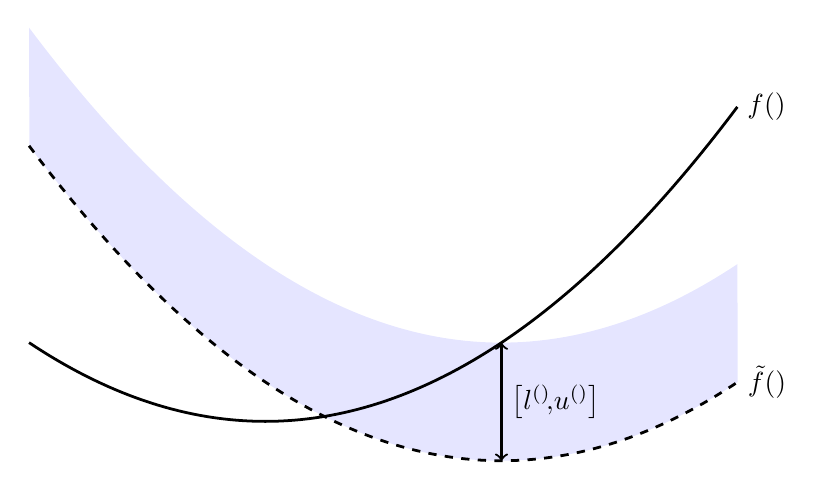
\begin{tikzpicture}[x=3cm, y=1cm]
  			% Filled band around the quadratic curve with different boundary curves
			\fill[blue!10] 
			(-1, 5) -- plot[domain=-2:1, samples=100] ({\x+1}, {\x*\x + 1}) -- 
			plot[domain=1:-2, samples=100] ({\x+1}, {\x*\x - 0.5}) -- cycle;
  			\node[anchor=west] at (2, 4) {$f(\weights)$};
  			\draw[line width=1, domain=-2:1, samples=100,dashed] plot  ({\x+1}, {\x*\x -0.5}) node[right] {$\tilde{f}(\weights)$};
   			\draw[line width=1, domain=-1:2, samples=100] plot ({\x}, {\x*\x});
 	 		\draw[<->, thick] (1, -0.5) -- (1, 1) node[midway, right] {$\big[ l^{(\weights)}\!,\!u^{(\weights)} \big]$};
			\end{tikzpicture}
			{\selectlanguage{greek}
			\caption{\foreignlanguage{greek}{Οι μέθοδοι} \glsentryuserii{ml} \foreignlanguage{greek}{μαθαίνουν} \glsentryuseriii{modelparams} $\weights$ 
			\foreignlanguage{greek}{χρησιμοποιώντας κάποια εκτίμηση του $f(\weights)$ για το τελικό κριτήριο
			επίδοσης $\bar{f}(\weights)$. Χρησιμοποιώντας ένα} \glsentryuseriii{probmodel}, \foreignlanguage{greek}{κανείς μπορεί να 
			χρησιμοποιήσει το $f(\weights)$ για να κατασκευάσει διαστήματα εμπιστοσύνης 
			$\big[ l^{(\weights)},  u^{(\weights)} \big]$ που περιέχουν το $\bar{f}(\weights)$  
			με υψηλή πιθανότητα. Το καλύτερο εύλογο μέτρο επίδοσης για μία συγκεκριμένη επιλογή $\weights$ των} \glsentryuserv{modelparams} 
			\foreignlanguage{greek}{είναι} $\tilde{f}(\weights) \defeq l^{(\weights)}$.} }
			\end{center}
		\end{figure}
		\foreignlanguage{greek}{Βλέπε επίσης:} \gls{ml}, \gls{modelparams}, \gls{erm}, \gls{loss}, \gls{dataset}, \gls{trainset}, \gls{risk}, \gls{hypothesis}, 
		\gls{probmodel}, \gls{probability}, \gls{objfunc}, \gls{srm}, \gls{ucb}.},
	first={\foreignlanguage{greek}{αισιοδοξία παρά την αβεβαιότητα}},
	text={\foreignlanguage{greek}{αισιοδοξία παρά την αβεβαιότητα}},
	user1={\foreignlanguage{greek}{αισιοδοξία παρά την αβεβαιότητα}} %nominative 
}

\newglossaryentry{acc}
{name={\foreignlanguage{greek}{ακρίβεια}},
	description={\foreignlanguage{greek}{Θεωρούμε}\index{\foreignlanguage{greek}{ακρίβεια}} 
		\glsentryuservi{datapoint} \foreignlanguage{greek}{που χαρακτηρίζονται από} \glsentryuservi{feature} $\featurevec \in \featurespace$ 
		\foreignlanguage{greek}{και μία κατηγορική} \glsentryuseriii{label}
		$\truelabel$ \foreignlanguage{greek}{που παίρνει τιμές από ένα πεπερασμένο} \glsentryuseriii{labelspace} $\labelspace$. 
		\foreignlanguage{greek}{Η ακρίβεις μίας} \glsentryuserii{hypothesis} 
		$\hypothesis: \featurespace \rightarrow \labelspace$, \foreignlanguage{greek}{όταν εφαρμόζεται στα}  
		\glsentryuservi{datapoint} \foreignlanguage{greek}{ενός} \glsentryuserii{dataset} 
		$\dataset = \big\{ \big(\featurevec^{(1)}, \truelabel^{(1)} \big), \ldots, \big(\featurevec^{(\samplesize)},\truelabel^{(\samplesize)}\big) \big\}$, 
		\foreignlanguage{greek}{ορίζεται τότε ως} 
		$$1 - (1/\samplesize)\sum_{\sampleidx=1}^{\samplesize} \lossfunczo{\big(\featurevec^{(\sampleidx)},\truelabel^{(\sampleidx)}\big)}{\hypothesis}$$ 
		\foreignlanguage{greek}{χρησιμοποιώντας την} \glsentryuseriii{zerooneloss} $\lossfunczo{\cdot}{\cdot}$.\\
		\foreignlanguage{greek}{Βλέπε επίσης:} \gls{datapoint}, \gls{feature}, \gls{label}, \gls{labelspace}, \gls{hypothesis}, \gls{dataset}, \gls{zerooneloss}, 
		\gls{loss}, \gls{metric}.},
	first={\foreignlanguage{greek}{ακρίβεια}},
	text={\foreignlanguage{greek}{ακρίβεια}},
	user1={\foreignlanguage{greek}{ακρίβεια}}, %nominative
	user2={\foreignlanguage{greek}{ακρίβειας}}, %genitive
	user3={\foreignlanguage{greek}{ακρίβεια}} %accusative   
}

\newglossaryentry{outlier}
{name={\foreignlanguage{greek}{ακραία τιμή}}, 
	description={\foreignlanguage{greek}{Πολλές μέθοδοι}\index{\foreignlanguage{greek}{ακραία τιμή}} \glsentryuserii{ml}  
		\foreignlanguage{greek}{παρακινούνται από την} \glsentryuseriii{iidasspt}, \foreignlanguage{greek}{η οποία ερμηνεύει} 
		\glsentryuservi{datapoint} \foreignlanguage{greek}{ως} \glsentryuservi{realization} \glsentryuserii{iid} \glsentryuserv{rv} 
		\foreignlanguage{greek}{με κοινή} \glsentryuseriii{probdist}. \foreignlanguage{greek}{Η} \glsentryuseri{iidasspt} 
		\foreignlanguage{greek}{είναι χρήσιμη για εφαρμογές όπου οι στατιστικές ιδιότητες της διαδικασίας παραγωγής} 
		\glsentryuserii{data} \foreignlanguage{greek}{είναι στάσιμες (ή χρονικά αναλλοίωτες)} \cite{Brockwell91}. 
		\foreignlanguage{greek}{Ωστόσο, σε κάποιες εφαρμογές τα} \glsentryuseri{data} \foreignlanguage{greek}{αποτελούνται 
		από μια πλειοψηφία ομαλών} \glsentryuserv{datapoint} \foreignlanguage{greek}{που συμμορφώνονται με την} 
		\glsentryuseriii{iidasspt} \foreignlanguage{greek}{καθώς και από έναν μικρό αριθμό} \glsentryuserv{datapoint} 
		\foreignlanguage{greek}{που έχουν θεμελιωδώς διαφορετικές στατιστικές ιδιότητες συγκριτικά με τα ομαλά}  
        		\glsentryuservi{datapoint}. \foreignlanguage{greek}{Αναφερόμαστε σε ένα} \glsentryuseriii{datapoint} \foreignlanguage{greek}{που  
        		αποκλίνει ουσιαστικά από τις στατιστικές ιδιότητες των περισσότερων} \glsentryuserv{datapoint} \foreignlanguage{greek}{ως μία
		ακραία τιμή. Διαφορετικές μέθοδοι για την  ανίχνευση ακραίας τιμής χρησιμοποιούν διαφορετικά μέτρα για αυτή την 
		απόκλιση. Η θεωρία στατιστικής μάθησης μελετάει τα θεμελιώδη όρια στη δυνατότητα να μετριαστούν αξιόπιστα 
		οι ακραίες τιμές} \cite{doi:10.1137/0222052}, \cite{10.1214/20-AOS1961}.\\
       		\foreignlanguage{greek}{Βλέπε επίσης:} \gls{ml}, \gls{iidasspt}, \gls{datapoint}, \gls{realization}, \gls{iid}, \gls{rv}, \gls{probdist}, \gls{data}.},
	  first={\foreignlanguage{greek}{ακραία τιμή}}, 
	  text={\foreignlanguage{greek}{ακραία τιμή}},
	  user1={\foreignlanguage{greek}{ακραία τιμή}}, %nominative
  	  user2={\foreignlanguage{greek}{ακραίας τιμής}} %genitive  
}

\newglossaryentry{algorithm}
{name={\foreignlanguage{greek}{αλγόριθμος}},
 	description={\foreignlanguage{greek}{Ένας}\index{\foreignlanguage{greek}{αλγόριθμος}} 
		\foreignlanguage{greek}{αλγόριθμος} (algorithm) \foreignlanguage{greek}{είναι μία ακριβής, βήμα προς βήμα προδιαγραφή για την  
		παραγωγή μίας εξόδου} (output) \foreignlanguage{greek}{από μία συγκεκριμένη είσοδο} (input) \foreignlanguage{greek}{εντός ενός πεπερασμένου 
		αριθμού υπολογιστικών βημάτων} \cite{Cormen:2022aa}. \foreignlanguage{greek}{Για παράδειγμα, ένας αλγόριθμος για την εκπαίδευση ενός} 
		\glsentryuserii{linmodel} \foreignlanguage{greek}{περιγράφει ρητά πώς να μετασχηματιστεί ένα δεδομένο} \glsentryuseri{trainset} 
		\foreignlanguage{greek}{σε} \glsentryuservi{modelparams} \foreignlanguage{greek}{μέσω μίας ακολουθίας} 
		\glsentryuserv{gradstep}. \foreignlanguage{greek}{Για να μελετήσουμε αλγόριθμους ενδελεχώς, μπορούμε να τους αναπαραστήσουμε 
		(ή να τους προσεγγίσουμε) με διαφορετικές μαθηματικές δομές} \cite{Sipser2013}. \foreignlanguage{greek}{Μία προσέγγιση είναι να 
		αναπαραστήσουμε έναν αλγόριθμο ως μία συλλογή πιθανών εκτελέσεων. Κάθε μεμονωμένη εκτέλεση είναι τότε μία ακολουθία της  
		μορφής $${\rm input}, s_1, s_2, \ldots, s_T, {\rm output}.$$ Αυτή η ακολουθία ξεκινάει από μία είσοδο και προοδεύει μέσω ενδιάμεσων βημάτων 
		μέχρι να παραδοθεί μία έξοδος. Είναι κρίσιμο ότι ένας αλγόριθμος συμπεριλαμβάνει περισσότερα από απλώς μία αντιστοίχιση από είσοδο 
		σε έξοδο· περιλαμβάνει επίσης ενδιάμεσα υπολογιστικά βήματα} $s_1, \ldots, s_T$.\\
		\foreignlanguage{greek}{Βλέπε επίσης:} \gls{linmodel}, \gls{trainset}, \gls{modelparams}, \gls{gradstep}, \gls{model}, \gls{stochastic}.},
	first={\foreignlanguage{greek}{αλγόριθμος}},
	text={\foreignlanguage{greek}{αλγόριθμος}},
	user1={\foreignlanguage{greek}{αλγόριθμος}}, %nominative
	user2={\foreignlanguage{greek}{αλγόριθμου}}, %genitive 
	user3={\foreignlanguage{greek}{αλγόριθμο}}, %accusative
	user4={\foreignlanguage{greek}{αλγόριθμοι}}, %nominativepl 
	user5={\foreignlanguage{greek}{αλγόριθμων}}, %genitivepl
	user6={\foreignlanguage{greek}{αλγόριθμους}} %accusativepl 
}

\newglossaryentry{kmeans}
{name={\foreignlanguage{greek}{αλγόριθμος $k$-μέσων}}, 
	description={\foreignlanguage{greek}{Ο}\index{\foreignlanguage{greek}{αλγόριθμος $k$-μέσων}} 
		\glsentryuseri{algorithm} $k$-\foreignlanguage{greek}{μέσων} 
		($k$-means) \foreignlanguage{greek}{είναι μία μέθοδος} \glsentryuserii{hardclustering} \foreignlanguage{greek}{που αποδίδει κάθε} 
		\glsentryuseriii{datapoint} \foreignlanguage{greek}{ενός} \glsentryuserii{dataset} 
		\foreignlanguage{greek}{σε ακριβώς μία από τις $k$ διαφορετικές} \glsentryuservi{cluster}. \foreignlanguage{greek}{Η μέθοδος εναλλάσσεται
		μεταξύ της ενημέρωσης των αποδόσεων} \glsentryuserv{cluster} 
		\foreignlanguage{greek}{(με τη} \glsentryuseriii{cluster} \foreignlanguage{greek}{με την πλησιέστερη} \glsentryuseriii{mean}) 
		\foreignlanguage{greek}{και του επανυπολογισμού των} \glsentryuserv{mean} \foreignlanguage{greek}{των} 
		\glsentryuserv{cluster} \foreignlanguage{greek}{δεδομένων των ενημερωμένων αποδόσεων} \glsentryuserv{cluster} 
		\cite[\foreignlanguage{greek}{Κεφ.} 8]{MLBasics}. \\
		\foreignlanguage{greek}{Βλέπε επίσης:} \gls{mean}, \gls{algorithm}, \gls{hardclustering}, \gls{datapoint}, \gls{dataset}, \gls{cluster}.},
	first={\foreignlanguage{greek}{αλγόριθμος $k$-μέσων}},
	text={\foreignlanguage{greek}{αλγόριθμος $k$-μέσων}},
	user1={\foreignlanguage{greek}{αλγόριθμος $k$-μέσων}}, %nominative
	user2={\foreignlanguage{greek}{αλγόριθμου $k$-μέσων}} %genitive
}

\newglossaryentry{mutualinformation}
{name={\foreignlanguage{greek}{αμοιβαίες πληροφορίες}},
	description={\foreignlanguage{greek}{Οι}\index{\foreignlanguage{greek}{αμοιβαίες πληροφορίες}} 
		\foreignlanguage{greek}{αμοιβαίες πληροφορίες} (mutual information - MI) $\mutualinformation{\featurevec}{\truelabel}$ 
 		\foreignlanguage{greek}{μεταξύ δύο} \glsentryuserv{rv} $\featurevec$, $\truelabel$ \foreignlanguage{greek}{που ορίζονται στον ίδιο} 
		\glsentryuseriii{probspace} \foreignlanguage{greek}{δίνονται από}
 		\cite{coverthomas} $$\mutualinformation{\featurevec}{\truelabel} \defeq 
		\expect \left\{ \log \frac{p (\featurevec,\truelabel)}{p(\featurevec)p(\truelabel)} \right\}.$$ 
		\foreignlanguage{greek}{Αποτελεί μέτρο του πόσο καλά μπορούμε να εκτιμήσουμε την} $\truelabel$ \foreignlanguage{greek}{βάσει 
		μόνο του} $\featurevec$. \foreignlanguage{greek}{Μία μεγάλη τιμή του} $\mutualinformation{\featurevec}{\truelabel}$ 
		\foreignlanguage{greek}{υποδεικνύει ότι η} $\truelabel$ \foreignlanguage{greek}{μπο\-ρεί να προβλεφθεί καλά μόνο από το} $\featurevec$. 
		\foreignlanguage{greek}{Αυτή η} \glsentryuseri{prediction} \foreignlanguage{greek}{θα μπορούσε να προκύψει από μία} 
		\glsentryuseriii{hypothesis} \foreignlanguage{greek}{που μαθαίνεται από μία μέθοδο} \glsentryuserii{ml} 
		\foreignlanguage{greek}{βασισμένη στην} \glsentryuseriii{erm}.\\
		\foreignlanguage{greek}{Βλέπε επίσης:} \gls{rv}, \gls{probspace}, \gls{prediction}, \gls{hypothesis}, \gls{erm}, \gls{ml}.}, 
	first={\foreignlanguage{greek}{αμοιβαίες πληροφορίες}}, 
	text={\foreignlanguage{greek}{αμοιβαίες πληροφορίες}},
	user1={\foreignlanguage{greek}{αμοιβαίες πληροφορίες}}, %nominativepl
	user2={\foreignlanguage{greek}{αμοιβαίων πληροφοριών}} %genitivepl 
}
        
\newglossaryentry{ridgeregression}
{name={\foreignlanguage{greek}{αμφικλινής παλινδρόμηση}}, 
	description={\foreignlanguage{greek}{Η αμφικλινής}\index{\foreignlanguage{greek}{αμφικλινής παλινδρόμηση}} 
		\glsentryuseri{regression} \foreignlanguage{greek}{μαθαίνει τα} \glsentryuseriii{weights} $\weights$ \foreignlanguage{greek}{μίας γραμμικής} \gls{map} 
		\glsentryuserii{hypothesis} $\hypothesis^{(\weights)}(\featurevec)= \weights\,^{T} \featurevec$. \foreignlanguage{greek}{Η ποιότητα  
		μίας συγκεκριμένης επιλογής για τις} \glsentryuservi{modelparams} $\weights$ \foreignlanguage{greek}{μετριέται από το άθροισμα  
		των δύο συνιστωστών. Η πρώτη συνιστώσα είναι η μέση} \glsentryuseri{sqerrloss} 
		\foreignlanguage{greek}{που προκαλείται από την $\hypothesis^{(\weights)}$ σε ένα σύνολο}
		\glsentryuserv{labeled datapoint} \foreignlanguage{greek}{(δηλαδή το} \glsentryuseriii{trainset}). \foreignlanguage{greek}{Η δεύτερη συνιστώσα είναι  
		η ανηγμένη τετραγωνική Ευκλείδεια} \glsentryuseri{norm} $\regparam \| \weights \|^{2}_{2}$ \foreignlanguage{greek}{με μία} \glsentryuseriii{parameter} 
		\glsentryuserii{regularization} $\regparam > 0$. \foreignlanguage{greek}{Η προσθήκη $\regparam \| \weights \|^{2}_{2}$ στη μέση} 
	    	\glsentryuseriii{sqerrloss} \foreignlanguage{greek}{είναι ισοδύναμη με την αντικατάσταση αρχικών} \glsentryuserv{datapoint} \foreignlanguage{greek}{από τις} 
	    	\glsentryuservi{realization} \foreignlanguage{greek}{(άπειρα πολλών)} \glsentryuserii{iid} \glsentryuserv{rv} \foreignlanguage{greek}{που είναι 
		κεντρικές γύρω από αυτά τα} \glsentryuservi{datapoint} \foreignlanguage{greek}{(βλέπε} \gls{regularization}).\\
	    	\foreignlanguage{greek}{Βλέπε επίσης:} \gls{regression}, \gls{weights}, \gls{hypothesis}, \gls{map}, \gls{modelparams}, \gls{sqerrloss}, \gls{labeled datapoint}, 
		\gls{trainset}, \gls{norm}, \gls{regularization}, \gls{parameter}, \gls{datapoint}, \gls{realization}, \gls{iid}, \gls{rv}. },
	    first={\foreignlanguage{greek}{αμφικλινής παλινδρόμηση}},
	    text={ridge regression},
	    user1={\foreignlanguage{greek}{αμφικλινής παλινδρόμηση}}, %nominative
	    user2={\foreignlanguage{greek}{αμφικλινούς παλινδρόμησης}} %genitive   
}

\newglossaryentry{svd}
{name={\foreignlanguage{greek}{ανάλυση ιδιαζουσών τιμών}}, 
  	description={\foreignlanguage{greek}{Η ανάλυση ιδιαζουσών τιμών}\index{\foreignlanguage{greek}{ανάλυση ιδιαζουσών τιμών}} 
		(singular value decomposition - SVD) 
  		\foreignlanguage{greek}{για έναν πίνακα $\mA \in \mathbb{R}^{\samplesize \times \dimlocalmodel}$ 
		είναι μία παραγοντοποί\-ηση της μορφής  
		$$\mA = \mathbf{V} {\bm \Lambda} \mathbf{U}\,^{T}$$ 
		με ορθοκανονικούς πίνακες $\mV \in \mathbb{R}^{\samplesize \times \samplesize}$ 
		και} $\mU \in \mathbb{R}^{\dimlocalmodel \times \dimlocalmodel}$ \cite{GolubVanLoanBook}. 
		\foreignlanguage{greek}{Ο πίνακας ${\bm \Lambda} \in \mathbb{R}^{\samplesize \times \dimlocalmodel}$ είναι 
		μη μηδενικός μόνο κατά την κύρια διαγώνιο, της οποίας οι καταχωρίσεις $\Lambda_{\featureidx,\featureidx}$ 
		είναι μη αρνητικές και αναφέρονται ως ιδιάζουσες τιμές.} },
	first={\foreignlanguage{greek}{ανάλυση ιδιαζουσών τιμών}},
	text={\foreignlanguage{greek}{ανάλυση ιδιαζουσών τιμών}},
	user1={\foreignlanguage{greek}{ανάλυση ιδιαζουσών τιμών}}, %nominative
	user2={\foreignlanguage{greek}{ανάλυσης ιδιαζουσών τιμών}} %genitive  
}

\newglossaryentry{evd}
{name={\foreignlanguage{greek}{ανάλυση ιδιοτιμών}}, 
	description={\foreignlanguage{greek}{Η ανάλυση ιδιοτιμών}\index{\foreignlanguage{greek}{ανάλυση ιδιοτιμών}} 
		(eigenvalue decomposition - EVD) \foreignlanguage{greek}{για έναν τετραγωνικό πίνακα $\mA \in \mathbb{R}^{\dimlocalmodel \times \dimlocalmodel}$ 
		είναι μία παραγοντοποίηση της μορφής  
		$$\mA = \mathbf{V} {\bm \Lambda} \mathbf{V}^{-1}.$$ 
		Οι στήλες του πίνακα $\mV = \big( \vv^{(1)}, \ldots, \vv^{(\dimlocalmodel)} \big)$ είναι τα}  
		\glsentryuseriv{eigenvector} \foreignlanguage{greek}{του πίνακα $\mV$. Ο διαγώνιος πίνακας  
		${\bm \Lambda} = {\rm diag} \big\{ \eigval{1}, \ldots, \eigval{\dimlocalmodel} \big\}$ 
		περιέχει τις} \glsentryuservi{eigenvalue} $\eigval{\featureidx}$ \foreignlanguage{greek}{που αντιστοιχούν στα} \glsentryuservi{eigenvector} 
		$\vv^{(\featureidx)}$. \foreignlanguage{greek}{Σημείωση ότι η παραπάνω ανάλυση υπάρχει μόνο αν ο πίνακας $\mA$ είναι διαγωνοποιήσιμος.} \\
		\foreignlanguage{greek}{Βλέπε επίσης:} \gls{eigenvector}, \gls{eigenvalue}.},
	first={\foreignlanguage{greek}{ανάλυση ιδιοτιμών}},
	text={\foreignlanguage{greek}{ανάλυση ιδιοτιμών}},
	user1={\foreignlanguage{greek}{ανάλυση ιδιοτιμών}}, %nominative
	user2={\foreignlanguage{greek}{ανάλυσης ιδιοτιμών}} %genitive  
}

\newglossaryentry{pca}
{name={\foreignlanguage{greek}{ανάλυση κυρίων συνιστωσών}}, 
	description={\foreignlanguage{greek}{Η ανάλυση κυρίων συνιστωσών}\index{\foreignlanguage{greek}{ανάλυση κυρίων συνιστωσών}} 
		(principal component analysis - PCA) \foreignlanguage{greek}{καθορίζει έναν γραμμικό} \glsentryuseriii{featuremap}, \foreignlanguage{greek}{έτσι 
		ώστε τα νέα} \glsentryuseriv{feature} \foreignlanguage{greek}{να μας επιτρέπουν να ξανακατασκευάσουμε τα αρχικά} \glsentryuservi{feature} 
		\foreignlanguage{greek}{με το} \glsentryuseriii{minimum} 
		\foreignlanguage{greek}{σφάλμα ανακατασκευής} \cite{MLBasics}.\\
		\foreignlanguage{greek}{Βλέπε επίσης:} \gls{featuremap}, \gls{feature}, \gls{minimum}.},
	first={\foreignlanguage{greek}{ανάλυση κυρίων συνιστωσών}},
	text={principal component analysis},
	user1={\foreignlanguage{greek}{ανάλυση κυρίων συνιστωσών}}, %nominative
	user2={\foreignlanguage{greek}{ανάλυσης κυρίων συνιστωσών}} %genitive  
}

\newglossaryentry{iid}
{name={\foreignlanguage{greek}{ανεξάρτητες και ταυτόσημα κατανεμημένες}}, 
	description={\foreignlanguage{greek}{Μπορεί να είναι χρήσιμο να ερμηνεύσουμε}\index{\foreignlanguage{greek}{ανεξάρτητες και ταυτόσημα κατανεμημένες}} 
		\glsentryuservi{datapoint} $\datapoint^{(1)}, \ldots, \datapoint^{(\samplesize)}$ \foreignlanguage{greek}{ως}
		\glsentryuservi{realization} \foreignlanguage{greek}{ανεξάρτητων και ταυτόσημα κατανεμημένων} (independent and identically distributed - i.i.d.) 
		\glsentryuserv{rv} \foreignlanguage{greek}{με κοινή} \glsentryuseriii{probdist}. \foreignlanguage{greek}{Αν αυτές οι} \glsentryuseriv{rv} \foreignlanguage{greek}{είναι 
		συνεχούς τιμής, η από κοινού τους} \glsentryuseri{pdf} \foreignlanguage{greek}{είναι  
		$p\big(\datapoint^{(1)}, \ldots, \datapoint^{(\samplesize)} \big) = \prod_{\sampleidx=1}^{\samplesize} p \big(\datapoint^{(\sampleidx)}\big)$, 
		με την $p(\datapoint)$ να είναι η κοινή περιθωριακή} \glsentryuseri{pdf} \foreignlanguage{greek}{των υποκείμενων} \glsentryuserv{rv}.\\
		\foreignlanguage{greek}{Βλέπε επίσης:} \gls{datapoint}, \gls{realization}, \gls{rv}, \gls{probdist}, \gls{pdf}.},
	first={\foreignlanguage{greek}{ανεξάρτητες και ταυτόσημα κατανεμημένες}},
	text={\foreignlanguage{greek}{ανεξάρτητες και ταυτόσημα κατανεμημένες}},
	user1={\foreignlanguage{greek}{ανεξάρτητες και ταυτόσημα κατανεμημένες}}, %nominativepl
  	user2={\foreignlanguage{greek}{ανεξάρτητων και ταυτόσημα κατανεμημένων}}, %genitivepl  
	user3={\foreignlanguage{greek}{ανεξάρτητες και ταυτόσημα κατανεμημένες}} %accusativepl 
}

\newglossaryentry{reward}
{name={\foreignlanguage{greek}{ανταμοιβή}}, 
	description={\foreignlanguage{greek}{Μία ανταμοιβή αναφέρεται σε κάποια παρατηρούμενη}\index{\foreignlanguage{greek}{ανταμοιβή}}  
		\foreignlanguage{greek}{(ή μετρημένη) ποσότητα που μας επιτρέπει να εκτιμήσουμε την} \glsentryuseriii{loss}  
		\foreignlanguage{greek}{που προκύπτει από την} \glsentryuseriii{prediction} \foreignlanguage{greek}{(ή απόφαση) μίας} \glsentryuserii{hypothesis} 
		$\hypothesis(\featurevec)$. \foreignlanguage{greek}{Για παράδειγμα, σε μία εφαρμογή}  
		\glsentryuserii{ml} \foreignlanguage{greek}{σε αυτοοδηγούμενα οχήματα, η $\hypothesis(\featurevec)$ θα μπορούσε να αναπαριστά την τρέχουσα  
		κατεύθυνση οδήγησης ενός οχήματος. Θα μπορούσαμε να κατασκευάσουμε μία ανταμοιβή από τις μετρήσεις 
		ενός αισθητήρα σύγκρουσης που υποδεικνύει αν το όχημα κινείται προς ένα εμπόδιο. Ορίζουμε μία χαμηλή ανταμοιβή για την 
		κατεύ\-θυνση οδήγησης $\hypothesis(\featurevec)$ αν το όχημα κινείται επικίνδυνα προς ένα εμπόδιο.} \\
		\foreignlanguage{greek}{Βλέπε επίσης:} \gls{loss}, \gls{prediction}, \gls{hypothesis}, \gls{ml}.},
	first={\foreignlanguage{greek}{ανταμοιβή}}, 
	text={\foreignlanguage{greek}{ανταμοιβή}},
	user1={\foreignlanguage{greek}{ανταμοιβή}}, %nominative
	user2={\foreignlanguage{greek}{ανταμοιβής}}, %genitive  
	user3={\foreignlanguage{greek}{ανταμοιβή}} %accusative
} 

\newglossaryentry{objfunc}
{name={\foreignlanguage{greek}{αντικειμενική συνάρτηση}}, 
	description={\foreignlanguage{greek}{Μια αντικειμενική}\index{\foreignlanguage{greek}{αντικειμενική συνάρτηση}} 
		\glsentryuseri{function} \foreignlanguage{greek}{είναι μία} \gls{map} \foreignlanguage{greek}{που αποδίδει μία αριθμητική αντικειμενική τιμή 
		$f(\weights)$ σε κάθε επιλογή $\weights$ κάποιας μεταβλητής που θέλουμε να βελτιστοποιήσουμε  
		(βλέπε Σχ.} \ref{fig_obj_func_dict}). \foreignlanguage{greek}{Στο πλαίσιο της} \glsentryuserii{ml}, \foreignlanguage{greek}{η μεταβλητή 
		βελτιστοποίησης θα μπορούσε να είναι οι} \glsentryuseri{modelparams} \foreignlanguage{greek}{μίας} 
		\glsentryuserii{hypothesis} $\hypothesis^{(\weights)}$. 
		\foreignlanguage{greek}{Κοινές αντικειμενικές} \glsentryuseriv{function} \foreignlanguage{greek}{περιλαμβάνουν τη} \glsentryuseriii{risk} 
		\foreignlanguage{greek}{(δηλαδή την προσδοκώμενη} \glsentryuseriii{loss}) \foreignlanguage{greek}{ή την} \glsentryuseriii{emprisk} 
		\foreignlanguage{greek}{(δηλαδή τη μέση} \glsentryuseriii{loss} \foreignlanguage{greek}{πάνω σε ένα} \glsentryuseriii{trainset}). 
		\foreignlanguage{greek}{Οι μέθοδοι} \glsentryuserii{ml} \foreignlanguage{greek}{εφαρμόζουν τεχνικές βελτιστοποίησης,  
		όπως τις} \glsentryuseriii{gdmethods}, \foreignlanguage{greek}{για να βρούν την επιλογή $\weights$ με τη βέλτιστη τιμή  
		(π.χ., το} \glsentryuseriii{minimum} \foreignlanguage{greek}{ή το} \glsentryuseriii{maximum}) \foreignlanguage{greek}{της αντικειμενικής} 
		\glsentryuserii{function}. \\
		\begin{figure}[H]
			\begin{center}
			\begin{tikzpicture}[scale=1.0]
				% Axes
				\draw[->] (-0.5,0) -- (4.5,0) node[right] {$\weights$};
				\draw[->] (0,-0.5) -- (0,3.5);
				% Objective function curve
				\draw[thick,domain=0.3:4,smooth,variable=\x] 
				plot ({\x}, {0.5*(\x-2)^2 + 0.5});
				% Label the curve
				\node at (3.5,2.8) {$f(\weights)$};
			\end{tikzpicture} 
			\end{center}
		{\selectlanguage{greek}
		\caption{\foreignlanguage{greek}{Μία αντικειμενική} \glsentryuseri{function} \foreignlanguage{greek}{αντιστοιχεί κάθε πιθανή τιμή $\weights$ 
		μίας μεταβλητής βελτιστοποίησης, όπως οι} \glsentryuseri{modelparams} \foreignlanguage{greek}{ενός} \glsentryuserii{model} \glsentryuserii{ml}, 
		\foreignlanguage{greek}{σε μία τιμή που μετράει τη χρησιμότητα της} $\weights$.\label{fig_obj_func_dict}} }
		\end{figure} 
		\foreignlanguage{greek}{Βλέπε επίσης:} \gls{function}, \gls{map}, \gls{ml}, \gls{modelparams}, \gls{hypothesis}, \gls{risk}, \gls{loss}, \gls{emprisk}, 
		\gls{trainset}, \gls{gdmethods}, \gls{minimum}, \gls{maximum}, \gls{model}, \gls{lossfunc}.},
	first={\foreignlanguage{greek}{αντικειμενική συνάρτηση}},
	text={\foreignlanguage{greek}{αντικειμενική συνάρτηση}},
	user1={\foreignlanguage{greek}{αντικειμενική συνάρτηση}}, %nominative
  	user2={\foreignlanguage{greek}{αντικειμενικής συνάρτησης}}, %genitive  
	user3={\foreignlanguage{greek}{αντικειμενική συνάρτηση}} %accusative
}

\newglossaryentry{inverse}
{name={\foreignlanguage{greek}{αντίστροφος πίνακας}},
	description={\foreignlanguage{greek}{Ένας αντίστροφος πίνακας}\index{\foreignlanguage{greek}{αντίστροφος πίνακας}} 
		(inverse matrix) $\mA^{-1}$ \foreignlanguage{greek}{ορίζεται για έναν τετραγωνικό πίνακα  
 		$\mA \in \mathbb{R}^{n \times n}$ που είναι πλήρους τάξης, που σημαίνει ότι οι στήλες του είναι γραμμικά 
		ανεξάρτητες. Σε αυτή την περίπτωση, ο $\mA$ λέγεται ότι είναι αντιστρέψιμος, 
 		και ο αντίστροφός του ικανοποιεί 
 		\[
 		\mA \mA^{-1} = \mA^{-1} \mA = \mI.
 		\]  	
     		Ένας τετραγωνικός πίνακας είναι αντιστρέψιμος αν και μόνο αν η} \glsentryuseriv{det} \foreignlanguage{greek}{του 
		είναι μη μηδενική. Οι αντίστροφοι πίνακες είναι θεμελιώδεις στη λύση συστημάτων γραμμικών εξισώσεων 
		και στην κλειστής μορφής λύση} \glsentryuserii{linreg} \cite{Strang2007}, \cite{Horn91}. \foreignlanguage{greek}{Η 
		έννοια του αντίστροφου πίνακα μπορεί να επεκταθεί σε πίνακες που δεν είναι τετραγωνικοί ή πλήρους τάξης. 
		Μπορεί κανείς να ορίσει έναν \guillemotleft αριστερό αντίστροφο\guillemotright\ $\mB$ 
     		που ικανοποιεί $\mB \mA = \mI$ ή έναν \guillemotleft δεξιό αντίστροφο\guillemotright\ $\mC$ που 
		ικανοποιεί $\mA \mC = \mI$. Για γενικούς ορθογώνιους ή ιδιάζοντες πίνακες, ο} 
     		\glsentryuseri{pseudoinverse} Moore–Penrose $\mA^{+}$ \foreignlanguage{greek}{παρέχει μία ενοποιημένη έννοια 
		του γενικευμένου αντίστροφου πίνακα} \cite{GolubVanLoanBook}.
 		 \begin{figure}[H]
 			\centering
 			\begin{tikzpicture}[x=2cm,y=2cm]
 			% LEFT: Standard basis
 			\begin{scope}
 				\draw[->, thick] (0,0) -- (1,0) node[below right] {$\vx$};
 				\draw[->, thick] (0,0) -- (0,1) node[above left] {$\vy$};
 			\end{scope}
 			% CENTER: Transformed basis (by A)
 			\begin{scope}[shift={(2.0,0)}]
 				\coordinate (A) at (1.5,0.5);
 				\coordinate (B) at (-0.2,1.2);
				\draw[->, very thick, red] (0,0) -- (A) node[pos=0.5, below right] {$\mA \vx$};
 				\draw[->, very thick, red] (0,0) -- (B) node[above right] {$\mA \vy$};
 			\end{scope}
 			% RIGHT: Inverse transformation
 			\begin{scope}[shift={(4.9,0)}]
 				\draw[->, very thick, blue] (0,0) -- (1,0) node[pos=0.5, below] {$\mA^{-1} (\mA \vx) = \vx$};
 				\draw[->, very thick, blue] (0,0) -- (0,1) node[above] {$\mA^{-1} (\mA \vy) = \vy$};
 			\end{scope}
 			% Curved arrows between stages
 			\draw[->, thick, bend left=20] (1.2,0.4) to node[above] {$\mA$} (1.8,0.4);
 			\draw[->, thick, bend left=20] (3.8,0.4) to node[below] {$\mA^{-1}$} (4.4,0.4);
 			\end{tikzpicture}
			{\selectlanguage{greek}
 			\caption{\foreignlanguage{greek}{Ένας πίνακας $\mathbf{A}$ αναπαριστά έναν γραμμικό μετασχηματισμό 
			του $\mathbb{R}^{2}$. Ο αντίστροφος πίνακας $\mathbf{A}^{-1}$ αναπαριστά τον αντίστροφο 
			μετασχηματισμό.} \label{fig_matrix_inverse_dict}} }
 		\end{figure}
		\foreignlanguage{greek}{Βλέπε επίσης:} \gls{det}, \gls{linreg}, \gls{pseudoinverse}.},
	first={\foreignlanguage{greek}{αντίστροφος πίνακας}},
	text={\foreignlanguage{greek}{αντίστροφος πίνακας}},
	user1={\foreignlanguage{greek}{αντίστροφος πίνακας}}, %nominative 
}

\newglossaryentry{ucb}
{name={\foreignlanguage{greek}{άνω φράγμα εμπιστοσύνης (ΑΦΕ)}},
	description={\foreignlanguage{greek}{Θεωρούμε μία εφαρμογή}\index{\foreignlanguage{greek}{άνω φράγμα εμπιστοσύνης (ΑΦΕ)}} 
		\glsentryuserii{ml} \foreignlanguage{greek}{που απαιτεί την επιλογή, σε κάθε χρονικό βήμα $\iteridx$, μίας ενέργειας 
		$\action_{\iteridx}$ από ένα πεπερασμένο σύνολο εναλλακτικών $\actionset$.} \foreignlanguage{greek}{Η χρησιμότητα της 
		επιλογής της ενέργειας $\action_{\iteridx}$ ποσοτικοποιείται από ένα αριθμητικό σήμα} \glsentryuserii{reward} 
		$\reward^{(\action_{\iteridx})}$. \foreignlanguage{greek}{Ένα ευρέως χρησιμοποιούμενο} \glsentryuseri{probmodel} 
		\foreignlanguage{greek}{για αυτόν τον τύπο προβλήματος ακολουθιακής λήψης αποφάσεων είναι το περιβάλλον} 
		\glsentryuserii{stochastic} \gls{mab} \cite{Bubeck2012}. \foreignlanguage{greek}{Σε αυτό το} \glsentryuseriii{model}, 
		\foreignlanguage{greek}{η} \glsentryuseri{reward} $\reward^{(\action)}$ \foreignlanguage{greek}{θεωρείται ως η} 
		\glsentryuseri{realization} \foreignlanguage{greek}{μίας} \glsentryuserii{rv} \foreignlanguage{greek}{με άγνωστη} 
		\glsentryuseriii{mean} $\mu^{(\action)}$. \foreignlanguage{greek}{Ιδανικά, θα επιλέγαμε πάντα την ενέργεια με την 
		μεγαλύτερη αναμενόμενη} \glsentryuseriii{reward} $\mu^{(\action)}$, \foreignlanguage{greek}{αλλά αυτές οι}  
		\glsentryuseriv{mean} \foreignlanguage{greek}{είναι άγνωστες και πρέπει να εκτιμηθούν από παρατηρούμενα} \glsentryuseriii{data}. 
		\foreignlanguage{greek}{Το να επιλε\-χθεί απλά η ενέργεια με τη μεγαλύτερη εκτίμηση $\widehat{\mu}^{(\action)}$ 
		μπορεί να οδηγήσει σε υποβέλτιστα αποτελέσματα λόγω της} \glsentryuserii{uncertainty} \foreignlanguage{greek}{στην 
		εκτίμηση. Η στρατηγική ΑΦΕ} (upper confidence bound - UCB) \foreignlanguage{greek}{το αντιμετωπίζει αυτό 
		επιλέγοντας ενέργειες όχι μόνο με βάση τις εκτιμώμενες} \glsentryuservi{mean} \foreignlanguage{greek}{αλλά και
		ενσωματώνοντας έναν όρο που αντανακλά την} \glsentryuseriii{uncertainty} \foreignlanguage{greek}{σε αυτές τις 
		εκτιμήσεις—ευνοώντας ενέργειες με υψηλή πιθανή} \glsentryuseriii{reward} \foreignlanguage{greek}{και υψηλή} 
		\glsentryuseriii{uncertainty}. \foreignlanguage{greek}{Θεωρητικές εγγυήσεις για την επίδοση στρατηγικών ΑΦΕ, 
		συμπεριλαμβανομένων των ορίων λογαριθμικής} \gls{regret}, \foreignlanguage{greek}{καταδεικνύονται στο} \cite{Bubeck2012}.\\
		\foreignlanguage{greek}{Βλέπε επίσης:} \gls{ml}, \gls{reward}, \gls{probmodel}, \gls{stochastic}, \gls{mab}, \gls{model}, 
		\gls{realization}, \gls{rv}, \gls{mean}, \gls{data}, \gls{uncertainty}, \gls{regret}.},
	first={\foreignlanguage{greek}{άνω φράγμα εμπιστοσύνης}},
	text={\foreignlanguage{greek}{άνω φράγμα εμπιστοσύνης}},
	user1={\foreignlanguage{greek}{άνω φράγμα εμπιστοσύνης}}, %nominative
    	user2={\foreignlanguage{greek}{άνω φράγματος εμπιστοσύνης}} %genitive  
}

\newglossaryentry{trustAI}
{name={\foreignlanguage{greek}{αξιόπιστη τεχνητή νοημοσύνη (αξιόπιστη ΤΝ)}},
	description={\foreignlanguage{greek}{Εκτός από τις} \glsentryuseriii{compasp} \foreignlanguage{greek}{και τις} \glsentryuseriii{statasp}, 
		\foreignlanguage{greek}{μία τρίτη κύρια διάσταση σχεδιασμού μεθόδων}  
		\glsentryuserii{ml} \foreignlanguage{greek}{είναι η αξιοπιστία τους}\index{\foreignlanguage{greek}{αξιόπιστη τεχνητή νοημοσύνη (αξιόπιστη ΤΝ)}} 
		\cite{pfau2024engineeringtrustworthyaideveloper}. 
		\foreignlanguage{greek}{Η Ευρωπαϊκή Ένωση (ΕΕ) έχει διατυπώσει επτά βασικές απαιτήσεις για αξιόπιστη}  
		\glsentryuseriii{ai} (trustworthy artificial intelligence - trustworthy AI) \foreignlanguage{greek}{(που συνήθως χτίζουν πάνω σε 
		μεθόδους} \glsentryuserii{ml}) \cite{ALTAIEU}: 
		\begin{enumerate}[label=\arabic*)]
			\item \foreignlanguage{greek}{Ανθρώπινη παρέμβαση και εποπτεία·}
			\item \foreignlanguage{greek}{Τεχνική} \glsentryuseri{robustness} \foreignlanguage{greek}{και ασφάλεια·}
			\item \foreignlanguage{greek}{Ιδιωτικότητα και διακυβέρνηση των} \glsentryuserii{data}·
			\item \glsentryuseriv{transparency}·
			\item \foreignlanguage{greek}{Διαφορετικότητα, απαγόρευση των διακρίσεων και δικαιοσύνη·}
			\item \foreignlanguage{greek}{Κοινωνιακή και περιβαλλοντική ευημερία·}
			\item \foreignlanguage{greek}{Λογοδοσία.}
		\end{enumerate}
		\foreignlanguage{greek}{Βλέπε επίσης:} \gls{compasp}, \gls{statasp}, \gls{ml}, \gls{ai}, \gls{robustness}, \gls{data}, \gls{transparency}.},
	first={\foreignlanguage{greek}{αξιόπιστη τεχνητή νοημοσύνη (αξιόπιστη ΤΝ)}},
	text={\foreignlanguage{greek}{αξιόπιστη ΤΝ}},
	user1={\foreignlanguage{greek}{αξιόπιστη τεχνητή νοημοσύνη}}, %nominative
  	user2={\foreignlanguage{greek}{αξιόπιστης τεχνητής νοημοσύνης}}, %genitive 
	user3={\foreignlanguage{greek}{αξιόπιστη τεχνητή νοημοσύνη}} %accusative
}

\newglossaryentry{discrepancy}
{name={\foreignlanguage{greek}{απόκλιση}},
	description={\foreignlanguage{greek}{Θεωρούμε μία εφαρμογή}\index{\foreignlanguage{greek}{απόκλιση}} 
		\glsentryuserii{fl} \foreignlanguage{greek}{με} \gls{netdata} \foreignlanguage{greek}{που αναπαριστώνται από ένα}
		\glsentryuseriii{empgraph}. \foreignlanguage{greek}{Οι μέθοδοι} \glsentryuserii{fl} \foreignlanguage{greek}{χρησιμοποιούν 
		ένα μέτρο απόκλισης για να συκρίνουν} \gls{map}s \glsentryuserii{hypothesis} \foreignlanguage{greek}{από} \glsentryuservi{localmodel} 
		\foreignlanguage{greek}{σε κόμβους} $\nodeidx,\nodeidx'$, \foreignlanguage{greek}{συνδεδεμένοι με μία ακμή στο} \glsentryuseriii{empgraph}. \\
		\foreignlanguage{greek}{Βλέπε επίσης:} \gls{fl}, \gls{netdata}, \gls{empgraph}, \gls{hypothesis}, \gls{map}, \gls{localmodel}.},
	first={\foreignlanguage{greek}{απόκλιση}},
	text={\foreignlanguage{greek}{απόκλιση}},
	user1={\foreignlanguage{greek}{απόκλιση}}, %nominative
	user2={\foreignlanguage{greek}{απόκλισης}} %genitive 
}

 \newglossaryentry{kld}
 {name={\foreignlanguage{greek}{απόκλιση} Kullback-Leibler (\foreignlanguage{greek}{απόκλιση} KL)}, 
 	description={\foreignlanguage{greek}{Η απόκλιση}\index{\foreignlanguage{greek}{απόκλιση} Kullback-Leibler (\foreignlanguage{greek}{απόκλιση} KL)} 
		KL (Kullback-Leibler divergence - KL divergence) \foreignlanguage{greek}{είναι ένα ποσοτικό μέτρο του πόσο διαφορετική 
		είναι μία} \glsentryuseri{probdist} \foreignlanguage{greek}{από μία άλλη} \cite{coverthomas}.\\
		\foreignlanguage{greek}{Βλέπε επίσης:} \gls{probdist}. },
 	first={\foreignlanguage{greek}{απόκλιση} Kullback-Leibler (\foreignlanguage{greek}{απόκλιση} KL)},
	text={\foreignlanguage{greek}{απόκλιση} Kullback-Leibler},
	user1={\foreignlanguage{greek}{απόκλιση} Kullback-Leibler}, %nominative
  	user2={\foreignlanguage{greek}{απόκλισης} Kullback-Leibler} %genitive   
}

\newglossaryentry{renyidiv}
{name={\foreignlanguage{greek}{απόκλιση} R\'enyi}, 
	sort={Renyi},
	description={\foreignlanguage{greek}{Η απόκλιση} R\'enyi\index{\foreignlanguage{greek}{απόκλιση} R\'enyi} 
		\foreignlanguage{greek}{μετράει την (αν)ομοιότητα μεταξύ δύο} \glsentryuserv{probdist} \cite{RenyiInfo95}.\\
		\foreignlanguage{greek}{Βλέπε επίσης:} \gls{probdist}.}, 
	first={\foreignlanguage{greek}{απόκλιση} R\'enyi},
	text={\foreignlanguage{greek}{απόκλιση} R\'enyi},
	user1={\foreignlanguage{greek}{απόκλιση} R\'enyi}, %nominative
	user2={\foreignlanguage{greek}{απόκλισης} R\'enyi} %genitive
} 

\newglossaryentry{effdim}
{name={\foreignlanguage{greek}{αποτελεσματική διάσταση}},
	description={\foreignlanguage{greek}{Η αποτελεσματική διάσταση}\index{\foreignlanguage{greek}{αποτελεσματική διάσταση}} 
		$\effdim{\hypospace}$ \foreignlanguage{greek}{ενός ά\-πειρου} \glsentryuserii{hypospace} $\hypospace$ \foreignlanguage{greek}{είναι ένα μέτρο του μεγέθους του. 
		Σε γενικές γραμμές, η αποτελεσματική διάσταση είναι ίση με τον αποτελεσματικό αριθμό ανεξάρτητων} 
		\glsentryuserii{modelparams} \foreignlanguage{greek}{που μπορούν να ρυθμιστούν. Αυτές οι}
		\glsentryuseriv{parameter} \foreignlanguage{greek}{μπορεί να είναι συντελεστές που χρησιμοποιούνtαι σε μία} \gls{linearmap} 
		\foreignlanguage{greek}{ή τα} \glsentryuseri{weights} \foreignlanguage{greek}{και οι όροι} \glsentryuserii{bias} \foreignlanguage{greek}{ενός} \glsentryuserii{ann}.\\
		\foreignlanguage{greek}{Βλέπε επίσης:} \gls{hypospace}, \gls{modelparams}, \gls{parameter}, \gls{linearmap}, \gls{weights}, \gls{bias}, \gls{ann}.},
	first={\foreignlanguage{greek}{αποτελεσματική διάσταση}},
	text={\foreignlanguage{greek}{αποτελεσματική διάσταση}},
	user1={\foreignlanguage{greek}{αποτελεσματική διάσταση}}, %nominative
	user2={\foreignlanguage{greek}{αποτελεσματικής διάστασης}} %genitive    
}

\newglossaryentry{loss}
{name={\foreignlanguage{greek}{απώλεια}}, 
	description={\foreignlanguage{greek}{Οι μέθοδοι} \glsentryuserii{ml}\index{\foreignlanguage{greek}{απώλεια}} 
		\foreignlanguage{greek}{χρησιμοποιούν μία} \glsentryuseriii{lossfunc} $\lossfunc{\datapoint}{\hypothesis}$ \foreignlanguage{greek}{για 
		να μετρήσουν το σφάλμα που προκαλείται από την εφαρμογή μίας  
		συγκεκριμένης} \glsentryuserii{hypothesis} \foreignlanguage{greek}{σε ένα συγκεκριμένο} \glsentryuseriii{datapoint}. \foreignlanguage{greek}{Με 
		μία μικρή κατάχρηση του συμβολισμού, χρησιμοποιούμε τον όρο απώλεια και για την ίδια τη} \glsentryuseriii{lossfunc} $\loss$ 
		\foreignlanguage{greek}{και για τη συγκεκριμένη τιμή} $\lossfunc{\datapoint}{\hypothesis}$, \foreignlanguage{greek}{για ένα} 
		\glsentryuseriii{datapoint} $\datapoint$ \foreignlanguage{greek}{και μία} \glsentryuseriii{hypothesis} $\hypothesis$.\\
		\foreignlanguage{greek}{Βλέπε επίσης:} \gls{ml}, \gls{lossfunc}, \gls{hypothesis}, \gls{datapoint}.},
	first={\foreignlanguage{greek}{απώλεια}},
	text={loss},
	user1={\foreignlanguage{greek}{απώλεια}}, %nominative
	user2={\foreignlanguage{greek}{απώλειας}}, %genitive
	user3={\foreignlanguage{greek}{απώλεια}} %accusative 
}

\newglossaryentry{abserr}
{name={\foreignlanguage{greek}{απώλεια απόλυτου σφάλματος}},
	description={\foreignlanguage{greek}{Θεωρούμε ένα} \glsentryuseriii{datapoint} \foreignlanguage{greek}{με} 
		\glsentryuservi{feature} $\featurevec \in \featurespace$ \foreignlanguage{greek}{και αριθμητική} 
		\glsentryuseriii{label} $\truelabel \in \mathbb{R}$. \foreignlanguage{greek}{Η} \glsentryuseri{loss}\index{\foreignlanguage{greek}{απώλεια απόλυτου σφάλματος}} 
		\foreignlanguage{greek}{απόλυτου σφάλματος που προκαλείται από μία} \glsentryuseriii{hypothesis} $\hypothesis: \featurespace \rightarrow \mathbb{R}$ 
		\foreignlanguage{greek}{ορίζεται ως $|\truelabel - \hypothesis(\featurevec)|$, δηλαδή η απόλυτη διαφορά μεταξύ της} 
		\glsentryuserii{prediction} $\hypothesis(\featurevec)$ \foreignlanguage{greek}{και της αληθούς} \glsentryuserii{label} $\truelabel$.\\
		\foreignlanguage{greek}{Βλέπε επίσης:} \gls{datapoint}, \gls{feature}, \gls{label}, \gls{loss}, \gls{hypothesis}, \gls{prediction}.},
	first={\foreignlanguage{greek}{απώλεια απόλυτου σφάλματος}},
	text={\foreignlanguage{greek}{απώλεια απόλυτου σφάλματος}},
	user1={\foreignlanguage{greek}{απώλεια απόλυτου σφάλματος}}, %nominative
	user2={\foreignlanguage{greek}{απώλειας απόλυτου σφάλματος}}, %genitive  
	user3={\foreignlanguage{greek}{απώλεια απόλυτου σφάλματος}} %accusative 
}

\newglossaryentry{hingeloss}
{name={\foreignlanguage{greek}{απώλεια άρθρωσης}}, 
	description={\foreignlanguage{greek}{Θεωρούμε ένα}\index{\foreignlanguage{greek}{απώλεια άρθρωσης}} 
		\glsentryuseriii{datapoint} \foreignlanguage{greek}{που χαρακτηρίζεται από ένα} \glsentryuseriii{featurevec} $\featurevec \in \mathbb{R}^{\featuredim}$ 
		\foreignlanguage{greek}{και μία δυαδική} \glsentryuseriii{label} $\truelabel \in \{-1,1\}$. \foreignlanguage{greek}{Η} \glsentryuseri{loss} 
		\foreignlanguage{greek}{άρθρωσης που προκαλείται από μία} \gls{map} \glsentryuserii{hypothesis} $\hypothesis(\featurevec)$ 
		\foreignlanguage{greek}{πραγματικής τιμής ορίζεται ως} 
		\begin{equation} 
			\label{equ_hinge_loss_gls_dict}
			\lossfunc{(\featurevec,\truelabel)}{\hypothesis} \defeq \max \{ 0 , 1 - \truelabel \hypothesis(\featurevec) \}. 
		\end{equation}
		\begin{figure}[H]
		\begin{center}
		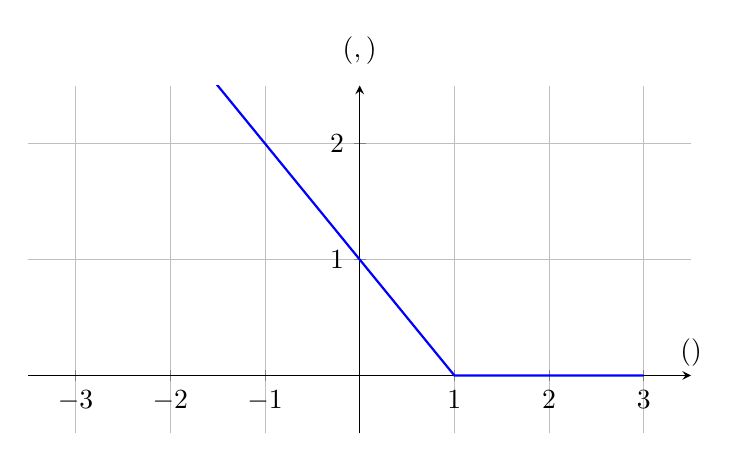
\begin{tikzpicture}
    			\begin{axis}[
        			axis lines=middle,
        			xlabel={$\truelabel\hypothesis(\featurevec)$},
        			ylabel={$\lossfunc{(\featurevec,\truelabel)}{\hypothesis}$},
 			xlabel style={at={(axis description cs:1.,0.3)}, anchor=north},  % Adjusted to be relative to axis end
        			ylabel style={at={(axis description cs:0.5,1.1)}, anchor=center}, % Corrected to vertical position, rotated for readability
        			xmin=-3.5, xmax=3.5,
        			ymin=-0.5, ymax=2.5,
        			xtick={-3, -2, -1, 0, 1, 2, 3},
        			ytick={0, 1, 2},
        			domain=-3:3,
        			samples=100,
        			width=10cm, height=6cm,
        			grid=both,
        			major grid style={line width=.2pt, draw=gray!50},
        			minor grid style={line width=.1pt, draw=gray!20},
        			legend pos=south west % Positions legend at the bottom left
    			]
        			\addplot[blue, thick] {max(0, 1-x)};
     			%   \addlegendentry{$\max(0, 1-x)$}
    			\end{axis}
		\end{tikzpicture}
		{\selectlanguage{greek}
		\caption{\foreignlanguage{greek}{Η} \glsentryuseri{loss} \foreignlanguage{greek}{άρθρωσης που προκαλείται από την} \glsentryuseriii{prediction} 
		$\hypothesis(\featurevec) \in \mathbb{R}$ \foreignlanguage{greek}{για ένα} \glsentryuseriii{datapoint} \foreignlanguage{greek}{με} 
		\glsentryuseriii{label} $\truelabel \in \{-1,1\}$. \foreignlanguage{greek}{Μία ομαλοποιημένη παραλλαγή της} \glsentryuserii{loss} 
		\foreignlanguage{greek}{άρθρωσης χρησιμοποιείται από τη} \glsentryuseriii{svm} \cite{LampertNowKernel}.}
		\label{fig_hingeloss_dict}}
		\end{center}
		\end{figure} 
	    	\foreignlanguage{greek}{Βλέπε επίσης:} \gls{datapoint}, \gls{featurevec}, \gls{label}, \gls{loss}, \gls{hypothesis}, \gls{map}, \gls{prediction}, \gls{svm}.},
	first={\foreignlanguage{greek}{απώλεια άρθρωσης}},
	text={\foreignlanguage{greek}{απώλεια άρθρωσης}},
	user1={\foreignlanguage{greek}{απώλεια άρθρωσης}}, %nominative
	user2={\foreignlanguage{greek}{απώλειας άρθρωσης}} %genitive   
}

\newglossaryentry{sqerrloss}
{name={\foreignlanguage{greek}{απώλεια τετραγωνικού σφάλματος}},
	description={\foreignlanguage{greek}{Η}\index{\foreignlanguage{greek}{απώλεια τετραγωνικού σφάλματος}} 
		\glsentryuseri{loss} \foreignlanguage{greek}{τετραγωνικού σφάλματος} (squared error loss) \foreignlanguage{greek}{μετράει το σφάλμα} 
		\glsentryuserii{prediction} \foreignlanguage{greek}{μίας} \glsentryuserii{hypothesis} $\hypothesis$ \foreignlanguage{greek}{όταν προβλέπει μία αριθμητική} 
		\glsentryuseriii{label} $\truelabel \in \mathbb{R}$ \foreignlanguage{greek}{από τα} \glsentryuservi{feature} $\featurevec$ 
		\foreignlanguage{greek}{ενός} \glsentryuserii{datapoint}. \foreignlanguage{greek}{Ορίζεται ως}  
		\begin{equation} 
			\nonumber
			\lossfunc{(\featurevec,\truelabel)}{\hypothesis} \defeq \big(\truelabel - \underbrace{\hypothesis(\featurevec)}_{=\predictedlabel} \big)^{2}. 
		\end{equation} 
		\foreignlanguage{greek}{Βλέπε επίσης:} \gls{loss}, \gls{prediction}, \gls{hypothesis}, \gls{label}, \gls{feature}, \gls{datapoint}.},
	first={\foreignlanguage{greek}{απώλεια τετραγωνικού σφάλματος}},
	text={\foreignlanguage{greek}{απώλεια τετραγωνικού σφάλματος}},
	user1={\foreignlanguage{greek}{απώλεια τετραγωνικού σφάλματος}}, %nominative
	user2={\foreignlanguage{greek}{απώλειας τετραγωνικού σφάλματος}}, %genitive
	user3={\foreignlanguage{greek}{απώλεια τετραγωνικού σφάλματος}} %accusative  
}

\newglossaryentry{huberloss}
{name={\foreignlanguage{greek}{απώλεια} Huber}, 
	description={\foreignlanguage{greek}{Η}\index{\foreignlanguage{greek}{απώλεια} Huber} 
		\glsentryuseri{loss} Huber \foreignlanguage{greek}{ενώνει την} \glsentryuseriii{sqerrloss} \foreignlanguage{greek}{και την} \glsentryuseriii{abserr}.\\
		\foreignlanguage{greek}{Βλέπε επίσης:} \gls{loss}, \gls{sqerrloss}, \gls{abserr}.},
	first={\foreignlanguage{greek}{απώλεια} Huber},
	text={\foreignlanguage{greek}{απώλεια} Huber},
	user1={\foreignlanguage{greek}{απώλεια} Huber}, %nominative
	user2={\foreignlanguage{greek}{απώλειας} Huber}, %genitive
	user3={\foreignlanguage{greek}{απώλεια} Huber} %accusative   
}

\newglossaryentry{condnr}
{name={\foreignlanguage{greek}{αριθμός συνθήκης}},
	description={\foreignlanguage{greek}{O αριθμός συνθήκης}\index{\foreignlanguage{greek}{αριθμός συνθήκης}} 
		$\kappa(\mathbf{Q}) \geq 1$ \foreignlanguage{greek}{ενός θετικά ορισμένου πίνακα $\mathbf{Q} \in \mathbb{R}^{\featurelen \times \featurelen}$ είναι ο  
		λόγος $\alpha /\beta $ μεταξύ της μεγαλύτερης $\alpha$ και της μικρότερης $\beta$} \glsentryuserii{eigenvalue} \foreignlanguage{greek}{του} 
		$\mathbf{Q}$. \foreignlanguage{greek}{O αριθμός συνθήκης είναι χρήσιμος για την ανάλυση μεθόδων} \glsentryuserii{ml}. 
		\foreignlanguage{greek}{Η υπολογιστική πολυπλοκότητα των} \glsentryuserii{gdmethods} \foreignlanguage{greek}{για} \glsentryuseriii{linreg} 
		\foreignlanguage{greek}{εξαρτάται κρίσιμα από τον αριθμό συνθήκης του πίνακα $\mQ = \mX \mX\,^{T}$, με τον} \glsentryuseriii{featuremtx} $\mX$ 
		\foreignlanguage{greek}{του} \glsentryuserii{trainset}. \foreignlanguage{greek}{Συνεπώς, από υπολογιστικής άποψης, προτιμούμε} \glsentryuservi{feature}  
		\glsentryuservi{datapoint}, \foreignlanguage{greek}{έτσι ώστε ο $\mQ$ να έχει έναν αριθμό συνθήκης κοντά στο} $1$.\\
		\foreignlanguage{greek}{Βλέπε επίσης:} \gls{eigenvalue}, \gls{ml}, \gls{gdmethods}, \gls{linreg}, \gls{featuremtx}, \gls{trainset}, \gls{feature}, \gls{datapoint}.},
	first={\foreignlanguage{greek}{αριθμός συνθήκης}},
	text={\foreignlanguage{greek}{αριθμός συνθήκης}},
	user1={\foreignlanguage{greek}{αριθμός συνθήκης}}, %nominative
	user2={\foreignlanguage{greek}{αριθμού συνθήκης}} %genitive  
}

\newglossaryentry{dataminprinc}
{name={\foreignlanguage{greek}{αρχή της ελαχιστοποίησης των δεδομένων}},
	description={\foreignlanguage{greek}{Ο Ευρωπαϊκός κανονι-\linebreakσμός για την προστασία}\index{\foreignlanguage{greek}{αρχή της ελαχιστοποίησης 
		των δεδομένων}} \glsentryuserii{data} \foreignlanguage{greek}{περιλαμβάνει μία αρχή ελαχιστο\-ποί\-ησης} \glsentryuserii{data}. 
		\foreignlanguage{greek}{Αυτή η αρχή απαιτεί έναν υπεύθυνο επεξεργασίας} \glsentryuserii{data} \foreignlanguage{greek}{για να περιορίσει  
		τη συλλογή προσωπικών πληροφοριών σε ό,τι είναι άμεσα σχετικό και απαραίτητο για την εκπλήρωση ενός προσδιορισμένου  
		σκοπού. Τα} \glsentryuseri{data} \foreignlanguage{greek}{πρέπει να φυλάσσονται μόνο για το χρονικό διάστημα που είναι απαραίτητα προκειμένου να 
		εκπληρωθεί αυτός ο σκοπός} \cite[\foreignlanguage{greek}{Άρθρο} 5(1)(c)]{GDPR2016}, \cite{EURegulation2018}.\\
		\foreignlanguage{greek}{Βλέπε επίσης:} \gls{data}.}, 
	first={data minimization principle},
	text={data minimization principle},
	user1={\foreignlanguage{greek}{αρχή της ελαχιστοποίησης των δεδομένων}}, %nominative
  	user2={\foreignlanguage{greek}{αρχής της ελαχιστοποίησης των δεδομένων}}, %genitive 
	user3={\foreignlanguage{greek}{αρχή της ελαχιστοποίησης των δεδομένων}}, %accusative
	user4={\foreignlanguage{greek}{Αρχή της ελαχιστοποίησης των δεδομένων}} %nominativecapital
}

\newglossaryentry{autoencoder}
{name={\foreignlanguage{greek}{αυτοκωδικοποιητής}},
	description={\foreignlanguage{greek}{Ένας αυτοκωδικοποιητής} (autoencoder)\index{\foreignlanguage{greek}{αυτοκωδικοποιητής}} 
		\foreignlanguage{greek}{είναι μία μέθοδος} \glsentryuserii{ml} \foreignlanguage{greek}{που μαθαίνει ταυτόχρονα έναν κωδικοποιητή} \gls{map} 
		$\hypothesis(\cdot) \in \hypospace$ \foreignlanguage{greek}{και έναν αποκωδικοποιητή} \gls{map} 
		$\hypothesis^{*}(\cdot) \in \hypospace^{*}$. \foreignlanguage{greek}{Είναι μία περίπτωση της} 
		\glsentryuserii{erm} \foreignlanguage{greek}{που χρησιμοποιεί μία} \glsentryuseriii{loss} \foreignlanguage{greek}{υπολογιζόμενη από το 
		σφάλμα ανακατασκευής} $\featurevec - \hypothesis^{*}\big(  \hypothesis \big( \featurevec \big) \big)$.\\
		\foreignlanguage{greek}{Βλέπε επίσης:} \gls{ml}, \gls{map}, \gls{erm}, \gls{loss}.},
	first={\foreignlanguage{greek}{αυτοκωδικοποιητής}},
	text={\foreignlanguage{greek}{αυτοκωδικοποιητής}}
}

\newglossaryentry{nodedegree}
{name={\foreignlanguage{greek}{βαθμός κόμβου}},
	description={\foreignlanguage{greek}{Ο βαθμός ενός κόμβου}\index{\foreignlanguage{greek}{βαθμός κόμβου}} 
		$\nodedegree{\nodeidx}$ $\nodeidx \in \nodes$ \foreignlanguage{greek}{σε έναν μη κατευ\-θυ\-νόμενο} 
		\glsentryuseriii{graph} \foreignlanguage{greek}{είναι ο αριθμός των} \glsentryuserii{neighbors}  
		\foreignlanguage{greek}{του, δηλαδή} $\nodedegree{\nodeidx} \defeq \big|\neighbourhood{\nodeidx}\big|$.\\
		\foreignlanguage{greek}{Βλέπε επίσης:} \gls{graph}, \gls{neighbors}.},
	first={\foreignlanguage{greek}{βαθμός κόμβου}},
	text={\foreignlanguage{greek}{βαθμός κόμβου}},
	user1={\foreignlanguage{greek}{βαθμός κόμβου}}, %nominative
  	user2={\foreignlanguage{greek}{βαθμού κόμβου}} %genitive 
}

\newglossaryentry{dob}
{name={\foreignlanguage{greek}{βαθμός συσχέτισης}},
	description={\foreignlanguage{greek}{Ο βαθμός συσχέτισης είναι ένας αριθμός που υποδεικνύει}\index{\foreignlanguage{greek}{βαθμός συσχέτισης}} 
		\foreignlanguage{greek}{το κατά πόσο ένα} \glsentryuseri{datapoint} 
		\foreignlanguage{greek}{ανήκει σε μία} \glsentryuseriii{cluster} \cite[\foreignlanguage{greek}{Κεφ.} 8]{MLBasics}. \foreignlanguage{greek}{Ο βαθμός  
		της συσχέτισης μπορεί να ερμηνευτεί ως μία μαλακή απόδοση} \glsentryuserii{cluster}. \foreignlanguage{greek}{Οι μέθοδοι} 
		\glsentryuserii{softclustering} \foreignlanguage{greek}{μπορούν να κωδικοποιήσουν τον βαθμό συσχέτισης με έναν πραγματικό  
		αριθμό στο διάστημα $[0,1]$. Η} \glsentryuseri{hardclustering} \foreignlanguage{greek}{προκύπτει ως η ακραία περίπτωη όταν ο βαθμός 
		συσχέτισης παίρνει μόνο τιμές} $0$ or $1$.\\
		\foreignlanguage{greek}{Βλέπε επίσης:} \gls{datapoint}, \gls{cluster}, \gls{softclustering}, \gls{hardclustering}.}, 
	first={\foreignlanguage{greek}{βαθμός συσχέτισης}},
	text={\foreignlanguage{greek}{βαθμός συσχέτισης}},
	user1={\foreignlanguage{greek}{βαθμός συσχέτισης}}, %nominative
    	user2={\foreignlanguage{greek}{βαθμού συσχέτισης}}, %genitive  
	user3={\foreignlanguage{greek}{βαθμό συσχέτισης}}, %accusative
    	user4={\foreignlanguage{greek}{βαθμοί συσχέτισης}}, %nominativepl 
	user5={\foreignlanguage{greek}{βαθμών συσχέτισης}}, %genitivepl
    	user6={\foreignlanguage{greek}{βαθ\-μούς συσχέτισης}} %accusativepl 
}

\newglossaryentry{deepnet}
{name={\foreignlanguage{greek}{βαθύ δίκτυο}},
	description={\foreignlanguage{greek}{Ένα βαθύ δίκτυο είναι ένα}\index{\foreignlanguage{greek}{βαθύ δίκτυο}} 
		\glsentryuseri{ann} \foreignlanguage{greek}{με έναν (σχετικά) μεγάλο αριθμό κρυφών στρωμάτων.  
		Η βαθιά μάθηση είναι ένας όρος-ομπρέλα για μεθόδους} \glsentryuserii{ml} \foreignlanguage{greek}{που 
		χρησιμοποιούν ένα βαθύ δίκτυο ως το} \glsentryuseriii{model} \foreignlanguage{greek}{τους} \cite{Goodfellow-et-al-2016}.\\
		\foreignlanguage{greek}{Βλέπε επίσης:} \gls{ann}, \gls{ml}, \gls{model}.},
	first={\foreignlanguage{greek}{βαθύ δίκτυο}},
	text={\foreignlanguage{greek}{βαθύ δίκτυο}},
	user1={\foreignlanguage{greek}{βαθύ δίκτυο}}, %nominative 
	user2={\foreignlanguage{greek}{βαθιού δικτύου}}, %genitive 
	user3={\foreignlanguage{greek}{βαθύ δίκτυο}}, %accusative 
	user4={\foreignlanguage{greek}{βαθιά δίκτυα}}, %nominativepl
	user5={\foreignlanguage{greek}{βαθιών δικτύων}}, %genitivepl
	user6={\foreignlanguage{greek}{βαθιά δίκτυα}} %accusativepl
}

\newglossaryentry{weights}
{name={\foreignlanguage{greek}{βάρη}},
	description={\foreignlanguage{greek}{Θεωρούμε έναν παραμετροποιημένο}\index{\foreignlanguage{greek}{βάρη}} 
		\glsentryuseriii{hypospace} $\hypospace$. \foreignlanguage{greek}{Χρησιμοποι\-ού\-με τον όρο βάρη για αριθμητικές} 
		\glsentryuseriii{modelparams} \foreignlanguage{greek}{που χρησιμοποιούνται 
		για να κλιμακώσουν} \glsentryuservi{feature} \foreignlanguage{greek}{ή τους μετασχηματισμούς τους προκειμένου να υπολογίσουμε 
		$\hypothesis^{(\weights)} \in \hypospace$. Ένα} \glsentryuseri{linmodel} 
		\foreignlanguage{greek}{χρησιμοποιεί βάρη $\weights=\big(\weight_{1}, \ldots, \weight_{\nrfeatures}\big)\,^{T}$ για να υπολογίσει 
		τον γραμμικό συνδυασμό $\hypothesis^{(\weights)}(\featurevec)= \weights\,^{T} \featurevec$. 
		Βάρη χρησιμοποιούνται επίσης σε} \glsentryuservi{ann} \foreignlanguage{greek}{για να σχηματιστούν γραμμικοί συνδυασμοί} 
		\glsentryuserv{feature} \foreignlanguage{greek}{ή των εξόδων νευρώνων σε κρυφά στρώματα.} 
		\begin{figure}[H]
			\begin{center}
			\begin{tikzpicture}[neuron/.style={circle, draw, minimum size=1cm}, 
                    	thick, >=stealth]
			% Hidden layer neurons
			\node[neuron] (h1) at (0, 2) {$h_1$};
			\node[neuron] (h2) at (0, 0) {$h_2$};
			\node[neuron] (h3) at (0, -2) {$h_3$};
			% Common target coordinate to merge arrows
			\coordinate[right=3cm of h2] (outpoint);
			% Label the linear combination to the right of the arrow tips
			\node[anchor=west] at ([xshift=0.2cm]outpoint) 
    			{$z = w_1 h_1 + w_2 h_2 + w_3 h_3$};
			% Arrows from hidden neurons to common point
			\draw[->] (h1) -- node[above] {$w_1$} (outpoint);
			\draw[->] (h2) -- node[above] {$w_2$} (outpoint);
			\draw[->] (h3) -- node[below] {$w_3$} (outpoint);
			\end{tikzpicture}
			\end{center}
			{\selectlanguage{greek}
			\caption{\foreignlanguage{greek}{Ένα τμήμα ενός} \glsentryuserii{ann} \foreignlanguage{greek}{που περιέχει ένα κρυφό 
			στρώμα με εξόδους (ή ενεργοποιήσεις) $h_{1}$,$h_{2}$, και $h_{3}$. Αυτές οι έξοδοι συνδυάζονται γραμμικά για 
			να υπολογιστεί το $z$ που μπορεί να χρησιμποποιηθεί είτε ως έξοδος του} \glsentryuserii{ann} \foreignlanguage{greek}{είτε 
			ως είσοδος σε ένα άλλο στρώμα.} \label{fig_weights_dict}} }
		\end{figure}
		\foreignlanguage{greek}{Βλέπε επίσης:} \gls{hypospace}, \gls{modelparams}, \gls{feature}, \gls{linmodel}, \gls{ann}.},
	first={\foreignlanguage{greek}{βάρη}},
	text={\foreignlanguage{greek}{βάρη}},
	user1={\foreignlanguage{greek}{βάρη}}, %nominativepl 
	user2={\foreignlanguage{greek}{βαρών}}, %nominativepl 
	user3={\foreignlanguage{greek}{βάρη}} %accusativepl 
}

\newglossaryentry{edgeweight}
{name={\foreignlanguage{greek}{βάρος ακμής}},
	description={\foreignlanguage{greek}{Σε κάθε ακμή $\edge{\nodeidx}{\nodeidx'}$ ενός}\index{\foreignlanguage{greek}{βάρος ακμής}} 
		\glsentryuserii{empgraph} \foreignlanguage{greek}{αποδίδεται ένα μη αρνητικό βάρος ακμής  
		$\edgeweight_{\nodeidx,\nodeidx'}\geq0$. 
		Ένα μηδενικό βάρος ακμής $\edgeweight_{\nodeidx,\nodeidx'}=0$ υποδεικνύει την απουσία  
		μίας ακμής μεταξύ κόμβων} $\nodeidx, \nodeidx' \in \nodes$.\\
		\foreignlanguage{greek}{Βλέπε επίσης:} \gls{empgraph}.}, 
	first={\foreignlanguage{greek}{βάρος ακμής}},
	text={\foreignlanguage{greek}{βάρος ακμής}},
	user1={\foreignlanguage{greek}{βάρος ακμής}}, %nominative
	user2={\foreignlanguage{greek}{βάρους ακμής}}, %genitive  
	user3={\foreignlanguage{greek}{βάρος ακμής}} %accusative 
}

\newglossaryentry{baseline}
{name={\foreignlanguage{greek}{βάση αναφοράς}},
    description={Consider\index{\foreignlanguage{greek}{βάση αναφοράς}} 
	some \gls{ml} method that produces a learned \gls{hypothesis} (or trained \gls{model}) $\learnthypothesis \in \hypospace$. 
	We evaluate the quality of a trained \gls{model} 
    	by computing the average \gls{loss} on a \gls{testset}. But how can we assess 
    	whether the resulting \gls{testset} performance is sufficiently good? How can we 
    	determine if the trained \gls{model} performs close to optimal such that there is little point 
    	in investing more resources (for \gls{data} collection or computation) to improve it? 
    	To this end, it is useful to have a reference (or baseline) level against which 
    	we can compare the performance of the trained \gls{model}. Such a reference value 
    	might be obtained from human performance, e.g., the misclassification rate of dermatologists 
   	who diagnose cancer from visual inspection of skin \cite{SkinHumanAI}. Another source for a baseline is an existing, 
    	but for some reason unsuitable, \gls{ml} method. For example, the existing \gls{ml} method 
    	might be computationally too expensive for the intended \gls{ml} application. 
    	Nevertheless, its \gls{testset} error can still serve as a baseline. Another, somewhat more principled, 
    	approach to constructing a baseline is via a \gls{probmodel}. In many cases, given a \gls{probmodel} $p(\featurevec,\truelabel)$,  
    	we can precisely determine the \gls{minimum} achievable \gls{risk} among any hypotheses
    	(not even required to belong to the \gls{hypospace} $\hypospace$) \cite{LC}. 
    	This \gls{minimum} achievable \gls{risk} (referred to as the \gls{bayesrisk}) is the \gls{risk} 
    	of the \gls{bayesestimator} for the \gls{label} $\truelabel$ of a \gls{datapoint}, given
    	its \gls{feature}s $\featurevec$. Note that, for a given choice of \gls{lossfunc}, the 
    	\gls{bayesestimator} (if it exists) is completely determined by the \gls{probdist} $p(\featurevec,\truelabel)$ \cite[Ch. 4]{LC}. 
    	However, computing the \gls{bayesestimator} and \gls{bayesrisk} presents two 
    	main challenges:
    	\begin{enumerate}[label=\arabic*)]
    		\item The \gls{probdist} $p(\featurevec,\truelabel)$ is unknown and must be estimated from observed \gls{data}.
    		\item Even if $p(\featurevec,\truelabel)$ were known, computing the \gls{bayesrisk} exactly may be computationally 
		infeasible \cite{cooper1990computational}. 
   	\end{enumerate}
	A widely used \gls{probmodel} is the \gls{mvndist} $\pair{\featurevec}{\truelabel} \sim \mathcal{N}({\bm \mu},{\bm \Sigma})$ 
	for \gls{datapoint}s characterized by numeric \gls{feature}s and \gls{label}s.
	Here, for the \gls{sqerrloss}, the \gls{bayesestimator} is given by the posterior 
	\gls{mean} $\mu_{\truelabel|\featurevec}$ of the \gls{label} $\truelabel$, given the 
	\gls{feature}s $\featurevec$ \cite{LC}, \cite{GrayProbBook}. The corresponding \gls{bayesrisk} 
	is given by the posterior \gls{variance} 
	$\sigma^{2}_{\truelabel|\featurevec}$ (see Fig. \ref{fig_post_baseline_dict}).
	\begin{figure}[H]
		\begin{center}
		\begin{tikzpicture}
			% Axes
			\draw[->] (-1,0) -- (7,0) node[right] {$\truelabel$}; % x-axis
			% Gaussian distribution centered at \gaussiancenter with variance 1
			\draw[thick,domain=-1:7,smooth,variable=\x] 
			  plot ({\x}, {2*exp(-0.5*((\x-\gaussiancenter)^2))});
			% Dashed line indicating the mean of the Gaussian
			\draw[dashed] (\gaussiancenter,0) -- (\gaussiancenter,2.5);
			\node[anchor=south] at ([yshift=-5pt] \gaussiancenter,2.5) {\small $\mu_{\truelabel|\featurevec}$};
			% Double arrow indicating the variance
			\draw[<->,thick] (\gaussiancenter-1,1) -- (\gaussiancenter+1,1.0);
			\node[anchor=west] at ([yshift=2pt] \gaussiancenter,1.2) {\small $\sigma_{\truelabel|\featurevec}$};
			% Posterior variance label
			%\node[anchor=south east] at (\gaussiancenter-0.5,1.8) {\small Posterior Variance};
			% x-axis marks with crosses
			  % x-axis marks with crosses
  			\foreach \x in {0.5} {
				\node[red] at (\x, 0) {\bf \large $\times$};
 			 }
  			% h(x) label for the first cross
  			\node[anchor=north] at (0.5,-0.2) {\small $\learnthypothesis(\featurevec)$};
		  \end{tikzpicture}
		\end{center}
		\caption{If the \gls{feature}s and the \gls{label} of a \gls{datapoint} are drawn from a \gls{mvndist}, we 
		can achieve the \gls{minimum} \gls{risk} (under \gls{sqerrloss}) by using the \gls{bayesestimator} $\mu_{\truelabel|\featurevec}$ 
		to predict the \gls{label} $\truelabel$ of a \gls{datapoint} with \gls{feature}s $\featurevec$. The corresponding 
		\gls{minimum} \gls{risk} is given by the posterior \gls{variance} $\sigma^{2}_{\truelabel|\featurevec}$. We can use 
		this quantity as a baseline for the average \gls{loss} of a trained \gls{model} $\learnthypothesis$. \label{fig_post_baseline_dict}}
	\end{figure}
	\foreignlanguage{greek}{Βλέπε επίσης:} \gls{ml}, \gls{hypothesis}, \gls{model}, \gls{loss}, \gls{testset}, \gls{data}, \gls{probmodel}, \gls{minimum}, 
	\gls{risk}, \gls{hypospace}, \gls{bayesrisk}, \gls{bayesestimator}, \gls{label}, \gls{datapoint}, \gls{feature}, \gls{lossfunc}, \gls{probdist}, \gls{mvndist}, 
	\gls{sqerrloss}, \gls{mean}, \gls{variance}.},
    first={\foreignlanguage{greek}{βάση αναφοράς}},
    text={\foreignlanguage{greek}{βάση αναφοράς}},
    user1={\foreignlanguage{greek}{βάση αναφοράς}}, %nominative
    user2={\foreignlanguage{greek}{βάσης αναφοράς}} %genitive
}

\newglossaryentry{gradstep}
{name={\foreignlanguage{greek}{βήμα κλίσης}},
	description={Given a \gls{differentiable} 
		real-valued \gls{function} $f(\cdot): \mathbb{R}^{\nrfeatures} \rightarrow \mathbb{R}$ 
		and a vector $\weights \in \mathbb{R}^{\nrfeatures}$, the \gls{gradient} step\index{\foreignlanguage{greek}{βήμα κλίσης}} 
		updates $\weights$ by adding the scaled negative \gls{gradient} $\nabla f(\weights)$ to obtain 
		the new vector (see Fig. \ref{fig_basic_GD_step_single_dict})
		\begin{equation}
			\label{equ_def_gd_basic_dict} 
			\widehat{\weights}  \defeq \weights - \lrate \nabla f(\weights).
		\end{equation} 
		Mathematically, the \gls{gradient} step is an operator $\mathcal{T}^{(f,\lrate)}$ 
		that is paramet\-rized by the \gls{function} $f$ and the \gls{stepsize} $\lrate$. 
		\begin{figure}[H]
			\begin{center}
				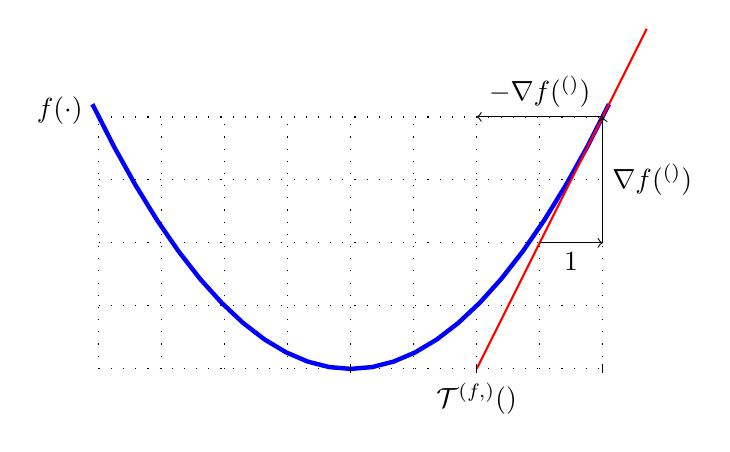
\begin{tikzpicture}[scale=0.8]
					\draw[loosely dotted] (-4,0) grid (4,4);
					\draw[blue, ultra thick, domain=-4.1:4.1] plot (\x,  {(1/4)*\x*\x});
					\draw[red, thick, domain=2:4.7] plot (\x,  {2*\x - 4});
					\draw[<-] (4,4) -- node[right] {$\nabla f(\weights^{(\itercntr)})$} (4,2);
					\draw[->] (4,4) -- node[above] {$-\lrate \nabla f(\weights^{(\itercntr)})$} (2,4);
					\draw[<-] (4,2) -- node[below] {$1$} (3,2) ;
					%\draw[->] (-4.25,0) -- (4.25,0) node[right] {$a$};
					\node[left] at (-4.1, 4.1) {$f(\cdot)$}; 
					\draw[shift={(0,0)}] (0pt,2pt) -- (0pt,-2pt) node[below] {$\overline{\weights}$};
					\draw[shift={(4,0)}] (0pt,2pt) -- (0pt,-2pt) node[below] {$\weights$};
					\draw[shift={(2,0)}] (0pt,2pt) -- (0pt,-2pt) node[below] {$\mathcal{T}^{(f,\lrate)}(\weights)$};
				\end{tikzpicture}
			\end{center}
			\caption{The basic \gls{gradient} step \eqref{equ_def_gd_basic_dict} maps a given vector $\weights$ 
			to the updated vector $\weights'$. It defines an operator 
			$\mathcal{T}^{(f,\lrate)}(\cdot): \mathbb{R}^{\nrfeatures} \rightarrow \mathbb{R}^{\nrfeatures}:
			 \weights \mapsto \widehat{\weights}$.}
			\label{fig_basic_GD_step_single_dict}
		\end{figure}
		Note that the \gls{gradient} step \eqref{equ_def_gd_basic_dict} optimizes locally—in a \gls{neighborhood} whose 
		size is determined by the \gls{stepsize} $\lrate$—a linear approximation 
		to the \gls{function} $f(\cdot)$. A natural \gls{generalization} of \eqref{equ_def_gd_basic_dict} is to locally 
		optimize the \gls{function} itself—instead of its linear approximation—such that
		\begin{align} 
		\label{equ_approx_gd_step_dict}
		\widehat{\weights} = \aargmin_{\weights' \in \mathbb{R}^{\dimlocalmodel}} f(\weights')\!+\!\frac{1}{\lrate}\normgeneric{\weights-\weights'}{2}^2. 
		\end{align}
		We intentionally use the same symbol $\lrate$ for the \gls{parameter} in \eqref{equ_approx_gd_step_dict} 
		as we used for the \gls{stepsize} in \eqref{equ_def_gd_basic_dict}. The larger the $\lrate$ we choose in 
		\eqref{equ_approx_gd_step_dict}, the more progress the update will make towards reducing the 
		\gls{function} value $f(\widehat{\weights})$. Note that, much like the \gls{gradient} step \eqref{equ_def_gd_basic_dict}, 
		the update \eqref{equ_approx_gd_step_dict} also defines an operator 
		that is parametrized by the \gls{function} $f(\cdot)$ and the \gls{learnrate} $\lrate$. For a \gls{convex} \gls{function} 
		$f(\cdot)$, this operator is known as the \gls{proxop} of $f(\cdot)$ \cite{ProximalMethods}.\\ 
		\foreignlanguage{greek}{Βλέπε επίσης:} \gls{differentiable}, \gls{function}, \gls{gradient}, \gls{stepsize}, \gls{neighborhood}, \gls{generalization}, 
		\gls{parameter}, \gls{learnrate}, \gls{convex}, \gls{proxop}.},
	first={\foreignlanguage{greek}{βήμα κλίσης}},
	text={\foreignlanguage{greek}{βήμα κλί\-σης}},
	user1={\foreignlanguage{greek}{βήμα κλίσης}}, %nominative
	user2={\foreignlanguage{greek}{βήματος κλίσης}}, %genitive
	user3={\foreignlanguage{greek}{βήμα κλίσης}}, %accusative 
	user4={\foreignlanguage{greek}{βήματα κλίσης}}, %nominativepl 
	user5={\foreignlanguage{greek}{βημάτων κλίσης}} %genitivepl  
}

\newglossaryentry{neighbors}
{name={\foreignlanguage{greek}{γείτονες}},
	description={\foreignlanguage{greek}{Οι γείτονες ενός κόμβου}\index{\foreignlanguage{greek}{γείτονες}} 
		$\nodeidx \in \nodes$ \foreignlanguage{greek}{εντός ενός} \glsentryuserii{empgraph} 
		\foreignlanguage{greek}{είναι εκείνοι οι κόμβοι $\nodeidx' \in \nodes \setminus \{ \nodeidx\}$ 
		που συνδέονται (μέσω μίας ακμής) με τον κόμβο} $\nodeidx$.\\
		\foreignlanguage{greek}{Βλέπε επίσης:} \gls{empgraph}.},
	first={\foreignlanguage{greek}{γείτονες}},
	text={\foreignlanguage{greek}{γείτονες}},
	user1={\foreignlanguage{greek}{γείτονες}}, %nominativepl
   	user2={\foreignlanguage{greek}{γειτόνων}}, %genitivepl 
	user3={\foreignlanguage{greek}{γείτονες}} %accusativepl
}

\newglossaryentry{neighborhood}
{name={\foreignlanguage{greek}{γειτονιά}},
	description={\foreignlanguage{greek}{Η γειτονιά ενός κόμβου}\index{\foreignlanguage{greek}{γειτονιά}} 
		$\nodeidx \in \nodes$ \foreignlanguage{greek}{είναι το υποσύνολο κόμβων που αποτελούνται από τους} 
		\glsentryuseriii{neighbors} \foreignlanguage{greek}{του} $\nodeidx$.\\
		\foreignlanguage{greek}{Βλέπε επίσης:} \gls{neighbors}.},
	first={neighborhood},
	text={neighborhood},
	user1={\foreignlanguage{greek}{γειτονιά}}, %nominative
   	user2={\foreignlanguage{greek}{γειτονιάς}} %genitive 
}

\newglossaryentry{gtv}
{name={\foreignlanguage{greek}{γενικευμένη ολική μεταβολή}}, 
	description={GTV (generalized total variation - GTV) is a\index{\foreignlanguage{greek}{γενικευμένη ολική μεταβολή}} 
		measure of the variation of trained \gls{localmodel}s $\localhypothesis{\nodeidx}$ 
		(or their \gls{modelparams} $\localparams{\nodeidx}$) assigned to the nodes $\nodeidx=1, \ldots, \nrnodes$ 
		of an undirected weighted \gls{graph} $\graph$ with edges $\edges$. Given a measure $\discrepancy{\hypothesis}{\hypothesis'}$ 
		for the \gls{discrepancy} between \gls{hypothesis} \gls{map}s $\hypothesis,\hypothesis'$, the GTV is 
		\begin{equation} 
			\nonumber
			\sum_{\edge{\nodeidx}{\nodeidx'}\in \edges} \edgeweight_{\nodeidx,\nodeidx'} 
			\discrepancy{\localhypothesis{\nodeidx}}{\localhypothesis{\nodeidx'}}.
		\end{equation}
		Here, $\edgeweight_{\nodeidx,\nodeidx'}>0$ denotes the weight of the undirected edge $\edge{\nodeidx}{\nodeidx'}\in \edges$.\\
		\foreignlanguage{greek}{Βλέπε επίσης:} \gls{localmodel}, \gls{modelparams}, \gls{graph}, \gls{discrepancy}, \gls{hypothesis}, \gls{map}.},
	first={\foreignlanguage{greek}{γενικευμένη ολική μεταβολή}},
	text={\foreignlanguage{greek}{γενικευμένη ολική μεταβολή}},
	user1={\foreignlanguage{greek}{γενικευμένη ολική μεταβολή}}, %nominative
  	user2={\foreignlanguage{greek}{γενικευμένης ολικής μεταβολής}} %genitive 
}

\newglossaryentry{generalization}
{name={\foreignlanguage{greek}{γενίκευση}}, 
	description={Generalization\index{\foreignlanguage{greek}{γενίκευση}} 
		refers to the ability of a \gls{model} trained on a \gls{trainset} to make accurate 
		\gls{prediction}s on new, unseen \gls{datapoint}s. This is a central goal of \gls{ml} and \gls{ai}, i.e.,
		to learn patterns that extend beyond the \gls{trainset}. Most \gls{ml} systems 
		use \gls{erm} to learn a \gls{hypothesis} $\learnthypothesis \in \hypospace$ by minimizing 
		the average \gls{loss} over a \gls{trainset} of \gls{datapoint}s $\datapoint^{(1)}, \ldots, \datapoint^{(\samplesize)}$, 
		denoted $\trainset$. However, success on the \gls{trainset} does not guarantee success on 
		unseen \gls{data}—this discrepancy is the challenge of generalization. \\ To study generalization 
		mathematically, we need to formalize the notion of ``unseen'' \gls{data}. A widely used 
		approach is to assume a \gls{probmodel} for \gls{data} generation, such as the \gls{iidasspt}. 
		Here, we interpret \gls{datapoint}s as independent \gls{rv}s with an identical 
		\gls{probdist} $p(\datapoint)$. This \gls{probdist}, which is assumed fixed but unknown, 
		allows us to define the \gls{risk} of a trained \gls{model} $\learnthypothesis$ as the expected \gls{loss}
		\[
		\risk{\learnthypothesis}=\expect_{\datapoint \sim p(\datapoint)} \big\{ \loss(\learnthypothesis, \datapoint) \big\}.
		\]
		The difference between \gls{risk} $\risk{\learnthypothesis}$ and \gls{emprisk} $\emprisk{\learnthypothesis}{\trainset}$ 
		is known as the \gls{gengap}. Tools from \gls{probability} theory, such as \gls{concentrationinequ}s 
		and uniform convergence, allow us to bound this gap under certain conditions \cite{ShalevMLBook}.\\
		Generalization without \gls{probability}: \Gls{probability} theory is one way to study how well a 
		\gls{model} generalizes beyond the \gls{trainset}, but it is not the only way. Another option is to use 
		simple, deterministic changes to the \gls{datapoint}s in the \gls{trainset}. The basic idea is that a 
		good \gls{model} $\learnthypothesis$ should be robust, i.e., its \gls{prediction} $\learnthypothesis(\featurevec)$ 
		should not change much if we slightly change the \gls{feature}s $\featurevec$ of a \gls{datapoint} $\datapoint$. 
		\\[1mm] For example, an object detector trained on smartphone photos should still detect the object if a few 
		random pixels are masked \cite{OnePixelAttack}. Similarly, it should deliver the same result if we rotate 
		the object in the image \cite{MallatUnderstandingDeepLearning}. 
		  \begin{figure}[H]
		                   	\centering
		                   	\begin{tikzpicture}[scale=0.8]
							   \draw[lightblue, fill=lightblue, opacity=0.5] (3, 2) ellipse (6cm and 2cm);
								\node[black] at (6, 3) {$p(\datapoint)$};
		                   		\fill[blue] (1, 3) circle (4pt) node[below, xshift=0pt, yshift=0pt] {$\datapoint^{(1)}$};
		                   		\fill[blue] (5, 1) circle (4pt) node[below] {$\datapoint^{(2)}$};
		                   		\fill[blue] (1.6, 3) circle (3pt);
		                   		\fill[blue] (0.4, 3) circle (3pt);
		                   		\draw[<->, thin] (1, 3) -- (1.6, 3);
		                   		\draw[<->, thin] (1, 3) -- (0.4, 3);
		                   		\fill[blue] (5.6, 1) circle (3pt);
		                   		\fill[blue] (4.4, 1) circle (3pt);
		                   		\draw[<->, thin] (5, 1) -- (5.6, 1);
		                   		\draw[<->, thin] (5, 1) -- (4.4, 1);
		                   		\draw[black, thick, domain=0:6, smooth] plot (\x, {- 1*\x + 5});
		                   		\node[black] at (3, 2.5) [right] {$\learnthypothesis$};
		                   	\end{tikzpicture}
		                   	\caption{Two \gls{datapoint}s $\datapoint^{(1)},\datapoint^{(2)}$ that are used as a \gls{trainset} 
		                   		to learn a \gls{hypothesis} $\learnthypothesis$ via \gls{erm}. We can evaluate $\learnthypothesis$ 
		                   		outside $\trainset$ either by an \gls{iidasspt} with some underlying \gls{probdist} $p(\datapoint)$ 
		                   		or by perturbing the \gls{datapoint}s.}
		                   	\label{fig:polynomial_fit_dict}
		        \end{figure}
		     \foreignlanguage{greek}{Βλέπε επίσης:} \gls{model}, \gls{trainset}, \gls{prediction}, \gls{datapoint}, \gls{ml}, \gls{ai}, \gls{erm}, \gls{hypothesis}, 
		     \gls{loss}, \gls{data}, \gls{probmodel}, \gls{iidasspt}, \gls{rv}, \gls{probdist}, \gls{risk}, \gls{emprisk}, \gls{gengap}, \gls{probability}, 
		     \gls{concentrationinequ}, \gls{feature}.},
	first={\foreignlanguage{greek}{γενίκευση}},
	text={\foreignlanguage{greek}{γενίκευση}},
	user1={\foreignlanguage{greek}{γενίκευση}}, %nominative
  	user2={\foreignlanguage{greek}{γενίκευσης}} %genitive 
}

\newglossaryentry{gdpr}
{name={\foreignlanguage{greek}{γενικός κανονισμός για την προστασία δεδομένων (ΓΚΠΔ)}},
	description={\foreignlanguage{greek}{Ο ΓΚΠΔ}\index{\foreignlanguage{greek}{γενικός κανονισμός για την προστασία δεδομένων (ΓΚΠΔ)}} 
		(general data protection regulation - GDPR) \foreignlanguage{greek}{θεσπίστηκε από την ΕΕ και τέθηκε σε ισχύ από τις 25 Μαΐου 2018} \cite{GDPR2016}. 
		\foreignlanguage{greek}{Διαφυλάσσει την ιδιωτικότητα και τα δικαιώματα} \glsentryuserii{data} \foreignlanguage{greek}{των ατόμων στην  
		ΕΕ. Ο ΓΚΠΔ έχει σημαντικές επιπτώσεις για το πώς συλλέγονται} \glsentryuseriii{data}, \foreignlanguage{greek}{πώς 
		αποθηκεύονται, και πώς χρησιμοποιούνται στις εφαρμογές} \glsentryuserii{ml}. \foreignlanguage{greek}{Βασικές 
		διατάξεις περιλαμβάνουν τα εξής}:
		\begin{itemize}
			\item \glsentryuseriv{dataminprinc}: \foreignlanguage{greek}{Τα συστήματα} \glsentryuserii{ml} \foreignlanguage{greek}{θα πρέπει να 
			χρησιμοποιούν μόνο την απαραίτητη ποσότητα προσωπικών} \glsentryuserii{data} \foreignlanguage{greek}{για τον σκοπό τους.} 
			\item \glsentryuseriv{transparency} \foreignlanguage{greek}{και} \glsentryuseri{explainability}: \foreignlanguage{greek}{Τα συστήματα} 
			\glsentryuserii{ml} \foreignlanguage{greek}{θα πρέπει να επιτρέπουν στους χρήστες τους να κατανοούν πώς τα συστήματα παίρνουν 
			αποφάσεις που επηρεάζουν τους χρήστες.} 
			\item \foreignlanguage{greek}{Δικαιώματα των υποκειμένων των} \glsentryuserii{data}: \foreignlanguage{greek}{Οι χρήστες θα πρέπει να 
			έχουν την ευκαιρία να έχουν πρόσβαση, να διορθώνουν, και να διαγράφουν τα προσωπικά τους} \glsentryuseriii{data}, 
			\foreignlanguage{greek}{καθώς και να αντιτίθενται στην αυτοματοποιημένη λήψη αποφάσεων και στην κατάρτιση προφίλ.} 
			\item \foreignlanguage{greek}{Λογοδοσία: Οι οργανισμοί πρέπει να εξασφαλίζουν την εύρωστη ασφάλεια} \glsentryuserii{data} 
			\foreignlanguage{greek}{και να αποδεικνύουν συμμόρφωση μέσω τεκμηρίων και τακτικών ελέγχων.} 
		\end{itemize}
		\foreignlanguage{greek}{Βλέπε επίσης:} \gls{data}, \gls{ml}, \gls{dataminprinc}, \gls{transparency}, \gls{explainability}.}, 
	first={\foreignlanguage{greek}{γενικός κανονισμός για την προστασία δεδομένων (ΓΚΠΔ)}},
	text={\foreignlanguage{greek}{ΓΚΠΔ}},
	user1={\foreignlanguage{greek}{γενικός κανονισμός για την προστασία δεδομένων}}, %nominative
    	user2={\foreignlanguage{greek}{γενικού κανονισμού για την προστασία δεδομένων}} %genitive 
}

\newglossaryentry{linmodel}
{name={\foreignlanguage{greek}{γραμμικό μοντέλο}},
	description={Consider\index{\foreignlanguage{greek}{γραμμικό μοντέλο}} 
		an \gls{ml} application involving \gls{datapoint}s, each represented 
		by a numeric \gls{featurevec} $\featurevec \in \mathbb{R}^{\nrfeatures}$. A linear \gls{model} defines 
		a \gls{hypospace} consisting of all real-valued \gls{linearmap}s from $\mathbb{R}^{\nrfeatures}$ to $\mathbb{R}$ such that
		\begin{equation}
			\label{equ_def_lin_model_hypspace_dict}
			\linmodel{\nrfeatures} \defeq \left\{ \hypothesis: \mathbb{R}^{\nrfeatures} \rightarrow \mathbb{R} \mid \hypothesis(\featurevec) = \weights^{\top} \featurevec \text{ for some } \weights \in \mathbb{R}^{\nrfeatures} \right\}.
		\end{equation}
		Each value of $\nrfeatures$ defines a different \gls{hypospace}, corresponding to the number of 
		\gls{feature}s used to compute the \gls{prediction} $\hypothesis(\featurevec)$. The choice of 
		$\nrfeatures$ is often guided not only by \gls{compasp} (e.g., fewer features reduce computation) and 
		\gls{statasp} (e.g., more features typically reduce \gls{bias} and \gls{risk}), but also by \gls{interpretability}. 
		A linear \gls{model} using a small number of well-chosen \gls{feature}s is generally considered 
		more interpretable \cite{rudin2019stop}, \cite{Ribeiro2016}.
		The linear \gls{model} is attractive because it can typically be trained using scalable \gls{convex} \gls{optmethod}s 
		\cite{hastie01statisticallearning}, \cite{BertsekasNonLinProgr}. Moreover, linear \gls{model}s often permit rigorous 
		statistical analysis, including fundamental limits on the \gls{minimum} achievable \gls{risk} \cite{Wain2019}. 
		They are also useful for analyzing more complex, non-linear \gls{model}s such as \gls{ann}s. For instance, 
		a \gls{deepnet} can be viewed as the composition of a \gls{featuremap}—implemented by the input and 
		hidden layers—and a linear \gls{model} in the output layer. Similarly, a \gls{decisiontree} can be interpreted 
		as applying a one-hot encoded \gls{featuremap} based on \gls{decisionregion}s, followed by a linear 
		\gls{model} that assigns a \gls{prediction} to each region.
		More generally, any trained \gls{model} $\learnthypothesis \in \hypospace$ that is 
		\gls{differentiable} at some $\featurevec'$ can be locally approximated by a \gls{linearmap} 
		$g(\featurevec)$. Figure~\ref{fig_linapprox_dict} illustrates such a local linear approximation, 
		defined by the \gls{gradient} $\nabla \learnthypothesis(\featurevec')$. Note that the \gls{gradient} 
		is only defined where $\learnthypothesis$ is \gls{differentiable}.
		To ensure \gls{robustness} in the context of \gls{trustAI}, one may prefer \gls{model}s whose 
		associated \gls{map} $\learnthypothesis$ is Lipschitz continuous. A classic result in mathematical 
		analysis—Rademacher’s Theorem—states that if $\learnthypothesis$ is Lipschitz continuous with 
		some constant $L$ over an open set $\Omega \subseteq \mathbb{R}^{\nrfeatures}$, then $\learnthypothesis$ 
		is \gls{differentiable} almost everywhere in $\Omega$ \cite[Th.~3.1]{heinonen2005lectures}.
		\begin{figure}[H]
		\begin{center}
		\begin{tikzpicture}[x=0.5cm]
			\begin{axis}[
			hide axis,
			xmin=-3, xmax=6,
			ymin=0, ymax=6,
			domain=0:6,
			samples=100,
			width=10cm,
			height=6cm,
			clip=false
			]
			% Original nonlinear function h(x)
			\addplot[blue, thick, domain=-2:6] {2 + sin(deg(x))} 
			node[pos=0.5, above right, yshift=3pt] {$\learnthypothesis(\featurevec)$};
			% Tangent line as local linear approximation at x = 3
			% h(3) = 2 + sin(3), h'(3) = cos(3)
			\addplot[red, thick, domain=4.5:6.5] 
			{2 + sin(deg(6)) + cos(deg(6))*(x - 6)}
			node[pos=0.95, above right] {$g(\featurevec)$};
			% Mark point of approximation
			\addplot[mark=*] coordinates {(6, {2 + sin(deg(6))})};
			    % Vertical dashed line (ruler) at x = 3
			\addplot[dashed, gray] coordinates {(6,0) (6,2.4)};
			\node at (axis cs:6, -0.2) {$\featurevec'$};
			    % Plot the two points
			    % Coordinates of the two points
			\pgfmathsetmacro{\xA}{-1.5}
			\pgfmathsetmacro{\xB}{3}
			\pgfmathsetmacro{\yA}{2 + sin(deg(\xA))}
			\pgfmathsetmacro{\yB}{2 + sin(deg(\xB))}
			\addplot[mark=*, only marks] coordinates {(\xA, \yA) (\xB, \yB)};
			%	\node at (axis cs:\xA, \yA+0.2) {$A$};
			%	\node at (axis cs:\xB, \yB+0.2) {$B$};
			% Draw dashed lines from the points to the x and y axes
			\draw[dashed, gray] (axis cs:\xA,\yA) -- (axis cs:\xA,0);
			\draw[dashed, gray] (axis cs:\xB,\yB) -- (axis cs:\xB,0);
			\draw[dashed, gray] (axis cs:\xA,\yA) -- (axis cs:0,\yA);
			\draw[dashed, gray] (axis cs:\xB,\yB) -- (axis cs:0,\yB);
			 % Draw delta x
			\draw[<->, thick] (axis cs:\xA,-0.4) -- node[below] {$\normgeneric{\Delta \featurevec}{2}$} (axis cs:\xB,-0.4);
			% Draw delta y
			\draw[<->, thick] (axis cs:-2.4,\yA) -- node[left] {$\leq L \normgeneric{\Delta \featurevec}{2}$} (axis cs:-2.4,\yB);
			\end{axis}
			\vspace*{-10mm}
		\end{tikzpicture}
		\vspace*{-5mm}
		\end{center}
		\caption{A trained \gls{model} $\learnthypothesis(\featurevec)$ that is \gls{differentiable} at a point $\featurevec'$ 
		can be locally approximated by a \gls{linearmap} $g \in \linmodel{\nrfeatures}$. This local approximation 
		is determined by the \gls{gradient} $\nabla \learnthypothesis(\featurevec')$.}
		\label{fig_linapprox_dict}
		\end{figure}
		\foreignlanguage{greek}{Βλέπε επίσης:} \gls{ml}, \gls{datapoint}, \gls{featurevec}, \gls{model}, \gls{hypospace}, \gls{linearmap}, \gls{feature}, 
		\gls{prediction}, \gls{compasp}, \gls{statasp}, \gls{bias}, \gls{risk}, \gls{interpretability}, \gls{convex}, \gls{optmethod}, \gls{minimum}, \gls{ann}, 
		\gls{deepnet}, \gls{featuremap}, \gls{decisiontree}, \gls{decisionregion}, \gls{differentiable}, \gls{gradient}, \gls{robustness}, \gls{trustAI}, \gls{map}, \gls{lime}.}, 
	first={\foreignlanguage{greek}{γραμμικό μοντέλο}},
   	text={\foreignlanguage{greek}{γραμμικό μοντέλο}},
   	user1={\foreignlanguage{greek}{γραμμικό μοντέλο}}, %nominative
   	user2={\foreignlanguage{greek}{γραμμικού μοντέλου}}, %genitive
   	user3={\foreignlanguage{greek}{γραμμικό μοντέλο}}, %accusative
   	user4={\foreignlanguage{greek}{γραμμικά μοντέλα}}, %nominativepl
   	user5={\foreignlanguage{greek}{γραμμικών μοντέλων}}, %genitivepl
   	user6={\foreignlanguage{greek}{γραμμικά μοντέλα}} %accusativepl
}

\newglossaryentry{linreg}
{name={\foreignlanguage{greek}{γραμμική παλινδρόμηση}}, 
	description={\foreignlanguage{greek}{Η γραμμική}\index{\foreignlanguage{greek}{γραμμική παλινδρόμηση}} 
		\glsentryuseri{regression} \foreignlanguage{greek}{στοχεύει να μάθει μία γραμμική} \gls{map} \glsentryuserii{hypothesis} 
		\foreignlanguage{greek}{για να προβλέψει μία αριθμητική} \glsentryuseriii{label} \foreignlanguage{greek}{με βάση τα αριθμητικά} 
		\glsentryuservi{feature} \foreignlanguage{greek}{ενός} \glsentryuserii{datapoint}. \foreignlanguage{greek}{Η ποιότητα μίας γραμμικής} 
		\gls{map} \glsentryuserii{hypothesis} \foreignlanguage{greek}{μετράται χρησιμοποιώντας τη μέση}  
		\glsentryuseriii{sqerrloss} \foreignlanguage{greek}{που προκαλείται σε ένα σύνολο} \glsentryuserv{labeled datapoint}, 
		\foreignlanguage{greek}{στο οποίο αναφερόμαστε ως το} \glsentryuseri{trainset}.\\
		\foreignlanguage{greek}{Βλέπε επίσης:} \gls{regression}, \gls{hypothesis}, \gls{map}, \gls{label}, \gls{feature}, \gls{datapoint},  \gls{sqerrloss}, 
		\gls{labeled datapoint}, \gls{trainset}.},
	first={\foreignlanguage{greek}{γραμμική παλινδρόμηση}},
	text={\foreignlanguage{greek}{γραμμική παλινδρόμηση}},
	user1={\foreignlanguage{greek}{γραμμική παλινδρόμηση}}, %nominative
	user2={\foreignlanguage{greek}{γραμμικής παλινδρόμησης}}, %genitive   
	user3={\foreignlanguage{greek}{γραμμική παλινδρόμηση}} %accusative
}

\newglossaryentry{linclass}
{name={\foreignlanguage{greek}{γραμμικός ταξινομητής}}, 
	description={\foreignlanguage{greek}{Θεωρούμε}\index{\foreignlanguage{greek}{γραμμικός ταξινομητής}} 
		\glsentryuservi{datapoint} \foreignlanguage{greek}{που χαρακτηρίζονται από αριθμητικά} \glsentryuservi{feature} $\featurevec \in \mathbb{R}^{\nrfeatures}$ 
	    	\foreignlanguage{greek}{και μία} \glsentryuseriii{label} $\truelabel \in \labelspace$ \foreignlanguage{greek}{από κάποιον
		πεπερασμένο} \glsentryuseriii{labelspace} $\labelspace$. 
		\foreignlanguage{greek}{Ένας γραμμικός} \glsentryuseri{classifier} \foreignlanguage{greek}{χαρακτηρίζεται από 
		το γεγονός ότι έχει} \glsentryuservi{decisionregion} \foreignlanguage{greek}{που διαχωρίζονται από υπερεπίπεδα 
		στο} $\mathbb{R}^{\featuredim}$ \cite[\foreignlanguage{greek}{Κεφ.} 2]{MLBasics}.\\
		\foreignlanguage{greek}{Βλέπε επίσης:} \gls{datapoint}, \gls{feature}, \gls{label}, \gls{labelspace}, \gls{classifier}, \gls{decisionregion}.},
	first={\foreignlanguage{greek}{γραμμικός ταξινομητής}},
	text={\foreignlanguage{greek}{γραμμικός ταξινομητής}},
	user1={\foreignlanguage{greek}{γραμμικός ταξινομητής}}, %nominative
	user2={\foreignlanguage{greek}{γραμμικoύ ταξινομητή}}, %genitive
	user3={\foreignlanguage{greek}{γραμμικό ταξινομητή}} %accusative  
}

\newglossaryentry{graph}
{name={\foreignlanguage{greek}{γράφος}},
	description={\foreignlanguage{greek}{Ένας γράφος}\index{\foreignlanguage{greek}{γράφος}} 
		$\graph = \pair{\nodes}{\edges}$ \foreignlanguage{greek}{είναι 
		ένα ζεύγος που αποτελείται από ένα σύνολο κόμβων $\nodes$ και ένα σύνολο ακμών $\edges$. Στην πιο γενική του μορφή, ένας γράφος 
		προσδιορίζεται από μία} \gls{map} \foreignlanguage{greek}{που αποδίδει σε κάθε ακμή $\edgeidx \in \edges$ ένα ζεύγος κόμβων} \cite{RockNetworks}. 
		\foreignlanguage{greek}{Μία σημαντική οικογένεια γράφων εί\-ναι οι απλοί μη κατευθυνόμενοι γράφοι. Ένας απλός μη κατευθυνόμενος  
		γράφος προκύπτει από την ταυτοποίηση κάθε ακμής $\edgeidx \in \edges$ με δύο διαφορετικούς κόμβους $\{\nodeidx,\nodeidx'\}$. 
		Οι σταθμισμένοι γράφοι προσδιορίζουν επίσης αριθμητικά} \glsentryuseriii{weights} $\edgeweight_{\edgeidx}$ 
		\foreignlanguage{greek}{για κάθε ακμή} $\edgeidx \in \edges$.\\
		\foreignlanguage{greek}{Βλέπε επίσης:} \gls{map}, \gls{weights}.},
	first={\foreignlanguage{greek}{γράφος}},
	text={graph},
	user1={\foreignlanguage{greek}{γράφος}}, %nominative
  	user2={\foreignlanguage{greek}{γράφου}}, %genitive
	user3={\foreignlanguage{greek}{γράφο}}, %accusative  
	user4={\foreignlanguage{greek}{γράφοι}} %nominativepl  
}

 \newglossaryentry{simgraph}
 {name={\foreignlanguage{greek}{γράφος ομοιότητας}}, 
 	description={Some\index{\foreignlanguage{greek}{γράφος ομοιότητας}} \gls{ml} applications generate \gls{datapoint}s that 
 		are related by a domain-specific notion of similarity. These similarities can be 
 		represented conveniently using a similarity \gls{graph} $\graph = \big(\nodes \defeq \{1, \ldots, \samplesize\},\edges\big)$. 
 		The node $\sampleidx \in \nodes$ represents the $\sampleidx$-th \gls{datapoint}. Two 
 		nodes are connected by an undirected edge if the corresponding \gls{datapoint}s are similar.\\
		\foreignlanguage{greek}{Βλέπε επίσης:} \gls{ml}, \gls{datapoint}, \gls{graph}.},
 	first={\foreignlanguage{greek}{γράφος ομοιότητας}},
	text={\foreignlanguage{greek}{γράφος ομοιότητας}},
	user1={\foreignlanguage{greek}{γράφος ομοιότητας}}, %nominative
  	user2={\foreignlanguage{greek}{γράφου ομοιότητας}} %genitive   
}

\newglossaryentry{data}
{name={\foreignlanguage{greek}{δεδομένα}},
	 description={\foreignlanguage{greek}{Τα δεδομένα αναφέρονται σε αντικείμενα που φέρουν}\index{\foreignlanguage{greek}{δεδομένα}} 
	 	\foreignlanguage{greek}{πληροφορίες. Αυτά τα αντικείμενα μπορεί να είναι συγκεκριμένα φυσικά αντικείμενα 
		(όπως άνθρωποι ή ζώα) ή αφηρημένες έννοιες (όπως αριθμοί).  Συχνά χρησιμοποιούμε αναπαραστάσεις (ή 
	 	προσεγγίσεις) των αρχικών δεδομένων που είναι πιο βολικές για την επεξεργασία των δεδομένων. 
		Αυτές οι προσεγγίσεις χρησιμοποιούν διαφορετικές μαθηματικές δομές όπως σχέσεις που χρησιμοποιούνται 
		σε σχεσιακές βάσεις δεδομένων} \cite{codd1970relational}, \cite{silberschatz2019database}\\
		\foreignlanguage{greek}{Βλέπε επίσης:} \gls{model}, \gls{dataset}, \gls{datapoint}.}, 
	first={\foreignlanguage{greek}{δεδομένα}},
	text={data},
	user1={\foreignlanguage{greek}{δεδομένα}}, %nominativepl
  	user2={\foreignlanguage{greek}{δεδομένων}}, %genitivepl 
	user3={\foreignlanguage{greek}{δεδομένα}} %accusativepl 
}

\newglossaryentry{sample}
{name={\foreignlanguage{greek}{δείγμα}},
	description={\foreignlanguage{greek}{Μία}\index{\foreignlanguage{greek}{δείγμα}} 
		\foreignlanguage{greek}{πεπερασμένη ακολουθία (ή λίστα)} \glsentryuserv{datapoint}\linebreak $\datapoint^{(1)}, \ldots, \datapoint^{(m)}$ 
		\foreignlanguage{greek}{που προκύπτει ή ερμηνεύεται ως η} \glsentryuseri{realization} $\samplesize$ \glsentryuserii{iid} \glsentryuserv{rv}  
		\foreignlanguage{greek}{με κοινή} \glsentryuseriii{probdist} $p(\datapoint)$. \foreignlanguage{greek}{Το μήκος $\samplesize$ της  
		ακολουθίας αναφέρεται ως το} \glsentryuseri{samplesize}.\\
		\foreignlanguage{greek}{Βλέπε επίσης:} \gls{datapoint}, \gls{realization}, \gls{iid}, \gls{rv}, \gls{probdist}, \gls{samplesize}.},
	first={\foreignlanguage{greek}{δείγμα}},
	text={\foreignlanguage{greek}{δείγμα}},
	user1={\foreignlanguage{greek}{δείγμα}}, %nominative
	user2={\foreignlanguage{greek}{δείγματος}}, %genitive  
	user3={\foreignlanguage{greek}{δείγμα}}, %accusative
	user4={\foreignlanguage{greek}{δείγματα}}, %nominativepl
	user5={\foreignlanguage{greek}{δειγμάτων}}, %genitivepl
	user6={\foreignlanguage{greek}{δείγματα}}, %accusativepl
	user7={\foreignlanguage{greek}{δειγματικός}} %nominativeadjmasc
}

\newglossaryentry{decisiontree}
{name={\foreignlanguage{greek}{δέντρο αποφάσεων}}, 
	description={A\index{\foreignlanguage{greek}{δέντρο αποφάσεων}} 
		decision tree is a flow-chart-like representation of a \gls{hypothesis} \gls{map} $\hypothesis$. 
		More formally, a decision tree is a directed \gls{graph} containing a root node that reads 
		in the \gls{featurevec} $\featurevec$ of a \gls{datapoint}. The root node then forwards 
		the \gls{datapoint} to one of its child nodes based on some elementary test on the \gls{feature}s $\featurevec$. 
		If the receiving child node is not a leaf node, i.e., it has child nodes itself, 
	  	it represents another test. Based on the test result, the \gls{datapoint} is forwarded 
	   	to one of its descendants. This testing and forwarding of the \gls{datapoint} is continued 
	  	until the \gls{datapoint} ends up in a leaf node without any children.
		\begin{figure}[H]
		\begin{minipage}{.45\textwidth}
		\scalebox{1}{
		\begin{tikzpicture}
			\node[fill=black, circle, inner sep=2pt, label=above:{$\| \featurevec-\mathbf{u} \| \leq \varepsilon$?}] (A) {};	
			\node[fill=black, circle, inner sep=2pt, below left=1.5cm and 1cm of A, label=left:{$\hypothesis(\featurevec) = \predictedlabel_1$}] (B) {};
			\node[fill=black, circle, inner sep=2pt, below right=1.5cm and 1cm of A, label=right:{$\| \featurevec - \mathbf{v} \| \leq \varepsilon$?}] (C) {};
			\node[fill=black, circle, inner sep=2pt, below left=1.5cm and 1cm of C, label=left:{$\hypothesis(\featurevec) = \predictedlabel_2$}] (D) {};
			\node[fill=black, circle, inner sep=2pt, below right=1.5cm and 1cm of C, label=right:{$\hypothesis(\featurevec) =\predictedlabel_3$}] (E) {};
			\draw[line width=1.5pt, ->] (A) -- (B) node[midway, left] {no};
			\draw[line width=1.5pt, ->] (A) -- (C) node[midway, right] {yes};
			\draw[line width=1.5pt, ->] (C) -- (D) node[midway, left] {no};
			\draw[line width=1.5pt, ->] (C) -- (E) node[midway, right] {yes};
			\node at (0.7,-4.5) {\selectfont (a)};
		\end{tikzpicture}
		}
		\end{minipage}	
		\hspace*{15mm}
		\begin{minipage}{.45\textwidth}
		\hspace*{15mm}
		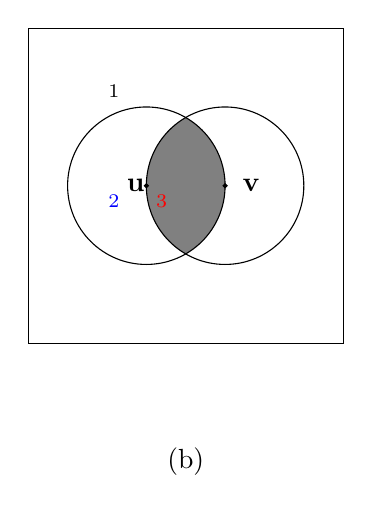
\begin{tikzpicture}
		\draw (-2,2) rectangle (2,-2);
		\begin{scope}
			\clip (-0.5,0) circle (1cm);
			\clip (0.5,0) circle (1cm);
			\fill[color=gray] (-2,1.5) rectangle (2,-1.5);
		\end{scope}
		\draw (-0.5,0) circle (1cm);
		\draw (0.5,0) circle (1cm);
		\draw[fill] (-0.5,0) circle [radius=0.025];
		\node [below right, red] at (-0.5,0) {$\predictedlabel_{3}$};
		\node [below left, blue] at (-0.7,0) {$\predictedlabel_{2}$};
		\node [above left] at (-0.7,1) {$\predictedlabel_{1}$};
		\node [left] at (-0.4,0) {$\mathbf{u}$};
		\draw[fill] (0.5,0) circle [radius=0.025];
		\node [right] at (0.6,0) {$\mathbf{v}$};
		\node at (0,-3.5) {\selectfont (b)};
		\end{tikzpicture}
		\end{minipage}
		\caption{(a) A decision tree is a flow-chart-like representation of a piece-wise constant \gls{hypothesis} $\hypothesis: \featurespace \rightarrow \mathbb{R}$.  
		Each piece is a \gls{decisionregion} $\decreg{\predictedlabel} \defeq \big\{ \featurevec \in  \featurespace: \hypothesis(\featurevec) = \predictedlabel \big\}$. 
		The depicted decision tree can be applied to numeric \gls{featurevec}s, i.e., $\featurespace \subseteq \mathbb{R}^{\dimlocalmodel}$. It is 
		parametrized by the threshold $\varepsilon>0$ and the vectors $\vu, \vv \in \mathbb{R}^{\dimlocalmodel}$. 
		(b) A decision tree partitions the \gls{featurespace} $\featurespace$ into \gls{decisionregion}s. Each \gls{decisionregion}  
		$\decreg{\hat{\truelabel}} \!\subseteq\!\featurespace$ corresponds to a specific leaf node in the decision tree.}
		\label{fig_decision_tree_dict}
		\end{figure} 
		\foreignlanguage{greek}{Βλέπε επίσης:} \gls{hypothesis}, \gls{map}, \gls{graph}, \gls{featurevec}, \gls{datapoint}, \gls{feature}, \gls{decisionregion}, \gls{featurespace}.},
	first={decision tree},
	text={decision tree},
	user1={\foreignlanguage{greek}{δέντρο αποφάσεων}}, %nominative
	user2={\foreignlanguage{greek}{δέντρου αποφάσεων}}, %genitive   
	user3={\foreignlanguage{greek}{δέντρο αποφάσεων}}, %accusative
	user4={\foreignlanguage{greek}{δέντρα αποφάσεων}}, %nominativepl  
	user5={\foreignlanguage{greek}{δέντρων αποφάσεων}}, %genitivepl
	user6={\foreignlanguage{greek}{δέντρα αποφάσεων}} %accusativepl  
}

\newglossaryentry{batch}
{name={\foreignlanguage{greek}{δέσμη}},
	description={\foreignlanguage{greek}{Στο πλαίσιο της}\index{\foreignlanguage{greek}{δέσμη}} 
		\glsentryuserii{stochGD}, \foreignlanguage{greek}{μία δέσμη αναφέρεται σε ένα τυχαία επιλεγμένο υποσύνολο 
		του γενικού} \glsentryuserii{trainset}. \foreignlanguage{greek}{Χρησιμοποιούμε τα} \glsentryuservi{datapoint} 
		\foreignlanguage{greek}{σε αυτό το υποσύνολο για να εκτιμήσουμε την} 
		\glsentryuseriii{gradient} \foreignlanguage{greek}{του} \glsentryuserii{trainerr} \foreignlanguage{greek}{και στη συνέχεια 
		να ενημερώσουμε τις} \glsentryuservi{modelparams}.\\
		\foreignlanguage{greek}{Βλέπε επίσης:} \gls{stochGD}, \gls{trainset}, \gls{datapoint}, \gls{gradient}, \gls{trainerr}, \gls{modelparams}.}, 
	first={\foreignlanguage{greek}{δέσμη}},
	text={\foreignlanguage{greek}{δέσμη}},
	user1={\foreignlanguage{greek}{δέσμη}}, %nominative
    	user2={\foreignlanguage{greek}{δέσμης}} %genitive  
}

\newglossaryentry{scatterplot}
{name={\foreignlanguage{greek}{διάγραμμα διασποράς}}, 
	description={\foreignlanguage{greek}{Μία}\index{\foreignlanguage{greek}{διάγραμμα διασποράς}} 
		\foreignlanguage{greek}{τεχνική οπτικοποίησης που απεικονίζει} \glsentryuservi{datapoint} \foreignlanguage{greek}{χρησιμοποιώντας 
		σημεία σε ένα δισδιάστατο επίπεδο. Το Σχ.} \ref{fig_scatterplot_temp_FMI_dict} \foreignlanguage{greek}{απεικονίζει ένα παράδειγμα 
		ενός διαγράμματος διασποράς.}   
		\begin{figure}[H]
			\begin{center}
				\begin{tikzpicture}[scale=1]
					\tikzset{x=2cm,y=2cm,every path/.style={>=latex},node style/.style={circle,draw}}
					\begin{axis}[axis x line=none,
						axis y line=none,
						ylabel near ticks,
						xlabel near ticks,
						enlarge y limits=true,
						xmin=-5, xmax=30,
						ymin=-5, ymax=30,
						width=6cm, height=6cm ]
						\addplot[only marks] table [x=mintmp, y=maxtmp, col sep = semicolon] {assets/FMIData1.csv};
						\node at (axis cs:26,2) [anchor=west] {$\feature$};
						\node at (axis cs:0,30) [anchor=west] {$\truelabel$};
						\draw[->] (axis cs:-5,0) -- (axis cs:30,0);
						\draw[->] (axis cs:0,-5) -- (axis cs:0,30);
					\end{axis}
				\end{tikzpicture}
				\vspace*{-10mm}
			\end{center}
			{\selectlanguage{greek}
			\caption{\foreignlanguage{greek}{Ένα διάγραμμα διασποράς κάποιων} \glsentryuserv{datapoint} \foreignlanguage{greek}{που 
				αντιπροσωπεύουν καθημερινές καιρικές συνθήκες στη Φινλανδία. Κάθε} 
				\glsentryuseri{datapoint} \foreignlanguage{greek}{χαρακτηρίζεται από την} \glsentryuseriv{minimum} 
				\foreignlanguage{greek}{θερμοκρασία της ημέρας $\feature$ ως το} 
				\glsentryuseriii{feature} \foreignlanguage{greek}{του και τη} \glsentryuserv{maximum} \foreignlanguage{greek}{θερμοκρασία 
				της ημέρας $\truelabel$ ως την} \glsentryuseriii{label} \foreignlanguage{greek}{του. 
				Οι θερμοκρασίες έχουν μετρηθεί στον σταθμό καιρού του} \glsentryuserii{fmi} \foreignlanguage{greek}{στο Ελσίνκι} 
				Kaisaniemi \foreignlanguage{greek}{κατά την περίοδο} 1.9.2024 - 28.10.2024.}
			\label{fig_scatterplot_temp_FMI_dict}}
			\vspace*{-3mm}
			\end{figure}
			\foreignlanguage{greek}{Ένα διάγραμμα διασποράς μπορεί να επιτρέψει τον οπτικό έλεγχο} \glsentryuserv{datapoint} 
			\foreignlanguage{greek}{που αναπαριστώνται φυσικά από} \glsentryuservi{featurevec} 
			\foreignlanguage{greek}{σε χώρους υψηλής διάστασης.}\\
			 \foreignlanguage{greek}{Βλέπε επίσης:} \gls{datapoint}, \gls{minimum}, \gls{feature}, \gls{maximum}, \gls{label}, \gls{fmi}, \gls{featurevec}, \gls{dimred}.},
		first={\foreignlanguage{greek}{διάγραμμα διασποράς}},
		text={\foreignlanguage{greek}{διάγραμμα διασποράς}},
		user1={\foreignlanguage{greek}{διάγραμμα διασποράς}}, %nominative
  		user2={\foreignlanguage{greek}{διαγράμματος διασποράς}} %genitive  
}

\newglossaryentry{risk}
{name={\foreignlanguage{greek}{διακινδύνευση}},
	description={\foreignlanguage{greek}{Θεωρούμε μία}\index{\foreignlanguage{greek}{διακινδύνευση}} 
		\glsentryuseriii{hypothesis} $\hypothesis$ \foreignlanguage{greek}{που χρησιμοποιείται για να προβλεφθεί η} \glsentryuseri{label} 
		$\truelabel$ \foreignlanguage{greek}{ενός} \glsentryuserii{datapoint} \foreignlanguage{greek}{βάσει των} \glsentryuserv{feature} $\featurevec$. 
		\foreignlanguage{greek}{Μετράμε την ποιότητα μίας συγκεκριμένης}  
		\glsentryuserii{prediction} \foreignlanguage{greek}{χρησιμοποιώντας μία} \glsentryuseriii{lossfunc} $\lossfunc{(\featurevec,\truelabel)}{\hypothesis}$. 
		\foreignlanguage{greek}{Αν ερμηνεύσουμε τα} \glsentryuservi{datapoint} \foreignlanguage{greek}{ως τις} \glsentryuservi{realization} 
		\glsentryuserii{iid} \glsentryuserv{rv}, \foreignlanguage{greek}{τότε και η 
		$\lossfunc{(\featurevec,\truelabel)}{\hypothesis}$ γίνεται η} \glsentryuseri{realization} 
		\foreignlanguage{greek}{μίας} \glsentryuserii{rv}. \foreignlanguage{greek}{Η} \glsentryuseri{iidasspt} \foreignlanguage{greek}{μας επιτρέπει 
		να ορίσουμε τη διακινδύνευση μίας} \glsentryuserii{hypothesis} 
		\foreignlanguage{greek}{ως την αναμενόμενη} \glsentryuseriii{loss} $\expect \big\{\lossfunc{(\featurevec,\truelabel)}{\hypothesis} \big\}$. 
		\foreignlanguage{greek}{Σημείωση ότι η διακινδύνευση της $\hypothesis$ εξαρτάται τόσο από την συγκεκριμένη επιλογή 
		για την} \glsentryuseriii{lossfunc} \foreignlanguage{greek}{όσο και από την} \glsentryuseriii{probdist} 
		\foreignlanguage{greek}{των} \glsentryuserv{datapoint}.\\
		\foreignlanguage{greek}{Βλέπε επίσης:} \gls{hypothesis}, \gls{label}, \gls{datapoint}, \gls{feature}, \gls{prediction}, \gls{lossfunc}, \gls{realization}, 
		\gls{iid} \gls{rv}, \gls{iidasspt}, \gls{loss}, \gls{probdist}.},
	first={\foreignlanguage{greek}{διακινδύνευση}},
	text={\foreignlanguage{greek}{διακινδύνευση}},
	user1={\foreignlanguage{greek}{διακινδύνευση}}, %nominative
    	user2={\foreignlanguage{greek}{διακινδύνευσης}}, %genitive 
	user3={\foreignlanguage{greek}{διακινδύνευση}}, %accusative 
	user4={\foreignlanguage{greek}{διακινδύνευσή}} %nominativeoraccussativedoublestress
}

\newglossaryentry{bayesrisk}
{name={\foreignlanguage{greek}{διακινδύνευση} Bayes},
	description={\foreignlanguage{greek}{Θεωρούμε ένα} \glsentryuseriii{probmodel} \foreignlanguage{greek}{με μία κοινή} \glsentryuseriii{probdist} 
		$p(\featurevec,\truelabel)$ \foreignlanguage{greek}{για τα} \glsentryuservi{feature} $\featurevec$ 
		\foreignlanguage{greek}{και την} \glsentryuseriii{label} $\truelabel$ \foreignlanguage{greek}{ενός} \glsentryuserii{datapoint}. 
		\foreignlanguage{greek}{Η}\index{\foreignlanguage{greek}{διακινδύνευση} Bayes} 
		\glsentryuseri{risk} Bayes (Bayes risk) \foreignlanguage{greek}{είναι η} \glsentryuseriv{minimum} \foreignlanguage{greek}{πιθανή} 
		\glsentryuseri{risk} \foreignlanguage{greek}{που μπορεί να επιτευχθεί από οποιαδήποτε} \glsentryuseriii{hypothesis} 
		$\hypothesis: \featurespace \rightarrow \labelspace$. \foreignlanguage{greek}{Οποιαδήποτε} \glsentryuseri{hypothesis} \foreignlanguage{greek}{που 
		επιτυγχάνει τη} \glsentryuseriii{risk} Bayes \foreignlanguage{greek}{αναφέρεται ως μία} \glsentryuseri{bayesestimator} \cite{LC}.\\
		\foreignlanguage{greek}{Βλέπε επίσης:} \gls{probmodel}, \gls{probdist}, \gls{feature}, \gls{label}, \gls{datapoint}, \gls{risk}, \gls{minimum}, 
		\gls{hypothesis}, \gls{bayesestimator}.},
	first={\foreignlanguage{greek}{διακινδύνευση} Bayes},
	text={\foreignlanguage{greek}{διακινδύνευση} Bayes},
	user1={\foreignlanguage{greek}{διακινδύνευση} Bayes}, %nominative
	user2={\foreignlanguage{greek}{διακινδύνευσης} Bayes} %genitive
}

\newglossaryentry{variance}
{name={\foreignlanguage{greek}{διακύμανση}},
	description={\foreignlanguage{greek}{Η διακύμανση μίας}\index{\foreignlanguage{greek}{διακύμανση}} 
		\glsentryuserii{rv} \foreignlanguage{greek}{πραγματικής τιμής $\feature$ ορίζεται ως η} \glsentryuseri{expectation} 
		$\expect\big\{ \big( x - \expect\{x \} \big)^{2} \big\}$ \foreignlanguage{greek}{της τετραγωνικής διαφοράς μεταξύ της $\feature$ 
		και της} \glsentryuserii{expectation} \foreignlanguage{greek}{της $\expect\{x \}$. Επεκτείνουμε αυτόν τον ορισμό σε} \glsentryuservi{rv} 
		\foreignlanguage{greek}{διανυσματικής τιμής $\featurevec$ 
		ως} $\expect\big\{ \big\| \featurevec - \expect\{\featurevec \} \big\|_{2}^{2} \big\}$.\\
		\foreignlanguage{greek}{Βλέπε επίσης:} \gls{rv}, \gls{expectation}.} ,
	first={\foreignlanguage{greek}{διακύμανση}},
	text={\foreignlanguage{greek}{διακύμανση}},
	user1={\foreignlanguage{greek}{διακύμανση}}, %nominative
   	user2={\foreignlanguage{greek}{διακύμανσης}}, %genitive 
	user3={\foreignlanguage{greek}{διακύμανση}} %accusative 
}

\newglossaryentry{featurevec}
{name={\foreignlanguage{greek}{διάνυσμα χαρακτηριστικών}},
	description={\foreignlanguage{greek}{Το διάνυσμα}\index{\foreignlanguage{greek}{διάνυσμα χαρακτηριστικών}} 
		\glsentryuserv{feature} \foreignlanguage{greek}{αναφέρεται σε ένα διάνυσμα $\vx = \big(x_{1}, \ldots, x_{\nrfeatures}\big)\,^{T}$ 
		του οποίου οι καταχωρίσεις είναι ξεχωριστά} \glsentryuservi{feature} $x_{1}, \ldots, x_{\nrfeatures}$. 
		\foreignlanguage{greek}{Πολλές μέθοδοι} \glsentryuserii{ml} \foreignlanguage{greek}{χρησιμοποιούν διανύσματα} 
		\glsentryuserv{feature} \foreignlanguage{greek}{που ανήκουν σε κάποιον} \glsentryuseriii{euclidspace} $\mathbb{R}^{\nrfeatures}$
		\foreignlanguage{greek}{πεπερασμένης διάστασης. Για κάποιες μεθόδους} 
		\glsentryuserii{ml}, \foreignlanguage{greek}{ωστόσο, μπορεί να είναι πιο βολικό να δουλεύουμε με διανύσματα} \glsentryuserv{feature} 
		\foreignlanguage{greek}{που ανήκουν σε έναν} \glsentryuseriii{vectorspace} \foreignlanguage{greek}{άπειρης διάστασης (π.χ. 
		βλέπε} \gls{kernelmethod}).\\
		\foreignlanguage{greek}{Βλέπε επίσης:} \gls{feature}, \gls{ml}, \gls{euclidspace}, \gls{vectorspace}.}, 
	first={\foreignlanguage{greek}{διάνυσμα χαρακτηριστικών}},
	text={\foreignlanguage{greek}{διάνυσμα χαρακτηριστικών}},
	user1={\foreignlanguage{greek}{διάνυσμα χαρακτηριστικών}}, %nominative
  	user2={\foreignlanguage{greek}{διανύσματος χαρακτηριστικών}}, %genitive
	user3={\foreignlanguage{greek}{διάνυσμα χαρακτηριστικών}}, %accusative     
	user4={\foreignlanguage{greek}{διανύσματα χαρακτηριστικών}}, %nominativepl
  	user5={\foreignlanguage{greek}{διανυσμάτων χαρακτηριστικών}}, %genitivepl
	user6={\foreignlanguage{greek}{διανύσματα χαρακτηριστικών}} %accusativepl
}

\newglossaryentry{privleakage}
{name={\foreignlanguage{greek}{διαρροή ιδιωτικότητας}},
	description={\foreignlanguage{greek}{Θεωρούμε μία εφαρμογή}\index{\foreignlanguage{greek}{διαρροή ιδιωτικότητας}} 
		\glsentryuserii{ml} \foreignlanguage{greek}{που επεξεργάζεται ένα} 
		\glsentryuseriii{dataset} $\dataset$ \foreignlanguage{greek}{και δίνει κάποια έξοδο, όπως οι} \glsentryuseriv{prediction} 
		\foreignlanguage{greek}{που προκύπτουν για νέα} \glsentryuservi{datapoint}. \foreignlanguage{greek}{Διαρροή ιδιωτικότητας ανακύπτει 
		αν η έξοδος φέρει πληροφορίες σχετικά με ένα ιδιωτικό (ή ευαίσθητο)} \glsentryuseriii{feature} \foreignlanguage{greek}{ενός} 
		\glsentryuserii{datapoint} \foreignlanguage{greek}{(που μπορεί να είναι άνθρωπος) ενός $\dataset$. Με βάση ένα} \glsentryuseriii{probmodel} 
		\foreignlanguage{greek}{για την παραγωγή} \glsentryuserii{data}, \foreignlanguage{greek}{μπορούμε να μετρήσουμε τη διαρροή ιδιωτικότητας 
		μέσω των} \glsentryuserii{mutualinformation} \foreignlanguage{greek}{μεταξύ της εξόδου και του ευαίσθητου} 
		\glsentryuserii{feature}. \foreignlanguage{greek}{Ένα άλλο ποιοτικό μέτρο διαρροής ιδιωτικότητας είναι η}  
		\glsentryuseri{diffpriv}. \foreignlanguage{greek}{Οι σχέσεις μεταξύ διαφορετικών μέτρων διαρροής ιδιωτικότητας έχουν μελετηθεί  
		στη βιβλιογραφία (βλέπε} \cite{InfThDiffPriv}).\\
		\foreignlanguage{greek}{Βλέπε επίσης:} \gls{ml}, \gls{dataset}, \gls{prediction}, \gls{datapoint}, \gls{feature}, \gls{probmodel}, \gls{data}, 
		\gls{mutualinformation}, \gls{diffpriv}, \gls{privattack}, \gls{gdpr}. }, 
	first={\foreignlanguage{greek}{διαρροή ιδιωτικότητας}}, 
	text={\foreignlanguage{greek}{διαρροή ιδιωτικότητας}},
	user1={\foreignlanguage{greek}{διαρροή ιδιωτικότητας}}, %nominative
   	user2={\foreignlanguage{greek}{διαρροής ιδιωτικότητας}} %genitive    
}

\newglossaryentry{kCV}
{name={\foreignlanguage{greek}{διασταυρούμενη επικύρωση $k$-συνόλων}},
	description={\foreignlanguage{greek}{Η} \glsentryuseri{kCV}
		($k$-fold cross-validation - $\nrfolds$-fold CV)\index{\foreignlanguage{greek}{διασταυρούμενη επικύρωση $k$-συνόλων}} 
		\foreignlanguage{greek}{είναι μία μέθοδος για τη μάθηση και} \glsentryuseriii{validation} 
		\foreignlanguage{greek}{μίας} \glsentryuserii{hypothesis}  
		\foreignlanguage{greek}{χρησιμοποιώντας ένα συγκεκριμένο} \glsentryuseriii{dataset}. 
		\foreignlanguage{greek}{Αυτή η μέθοδος 
		διαιρεί το} \glsentryuseriii{dataset} \foreignlanguage{greek}{ισότιμα σε $k$ υποσύνολα 
		και στη συνέχεια εκτελεί $k$ επαναλήψεις εκπαίδευσης} \glsentryuserii{model} 
		\foreignlanguage{greek}{(π.χ. μέσω της} \glsentryuserii{erm}) \foreignlanguage{greek}{και} \glsentryuserii{validation}. 
		\foreignlanguage{greek}{Κάθε επανάληψη χρησιμοποιεί ένα διαφορετικό υποσύνολο ως το} \glsentryuseriii{valset} 
		\foreignlanguage{greek}{και τα υπόλοιπα $k-1$ υποσύνολα ως} \glsentryuseriii{trainset}. 
		\foreignlanguage{greek}{Η τελική έξοδος είναι ο μέσος όρος των} \glsentryuserv{valerr} 
		\foreignlanguage{greek}{που προκύπτουν από τις $k$ επαναλήψεις.\\
		Βλέπε επίσης:} \gls{hypothesis}, \gls{dataset}, \gls{model}, \gls{erm}, \gls{validation}, \gls{valset}, \gls{trainset}, \gls{valerr}.},
	first={\foreignlanguage{greek}{διασταυρούμενη επικύρωση $k$-συνόλων}},
	text={\foreignlanguage{greek}{διασταυρούμενη επικύρωση $k$-συνόλων}}, 
	user1={\foreignlanguage{greek}{διασταυρούμενη επικύρωση $k$-συνόλων}}, %nominative
	user2={\foreignlanguage{greek}{διασταυρούμενης επικύρωσης $k$-συνόλων}} %genitive
}

\newglossaryentry{privfunnel}
{name={\foreignlanguage{greek}{δίαυλος ιδιωτικότητας}},
 	description={\foreignlanguage{greek}{Ο δίαυλος ιδιωτικότητας}\index{\foreignlanguage{greek}{δίαυλος ιδιωτικότητας}} 
		\foreignlanguage{greek}{είναι μία μέθοδος 
 		για τη μάθηση φιλικών προς την ιδιωτικότητα} \glsentryuserv{feature} \glsentryuserv{datapoint} \cite{PrivacyFunnel}.\\
		\foreignlanguage{greek}{Βλέπε επίσης:} \gls{feature}, \gls{datapoint}.},
 	first={\foreignlanguage{greek}{δίαυλος ιδιωτικότητας}},
 	text={\foreignlanguage{greek}{δίαυλος ιδιωτικότητας}},
 	user1={\foreignlanguage{greek}{δίαυλος ιδιωτικότητας}}, %nominative
 	user2={\foreignlanguage{greek}{διαύλου ιδιωτικότητας}} %genitive  
}

\newglossaryentry{transparency}
{name={\foreignlanguage{greek}{διαφάνεια}},
	description={Transparency\index{\foreignlanguage{greek}{διαφάνεια}} 
		is a fundamental requirement for \gls{trustAI} \cite{HLEGTrustworhtyAI}. In the context of \gls{ml} 
		methods, transparency is often used interchangeably with \gls{explainability} 
		\cite{JunXML2020}, \cite{gallese2023ai}. However, in the broader scope of \gls{ai} 
		systems, transparency extends beyond \gls{explainability} and includes providing information 
		about the system’s limitations, reliability, and intended use. 
		In medical diagnosis systems, transparency requires disclosing the confidence level 
		for the \gls{prediction}s delivered by a trained \gls{model}. In credit scoring, 
		\gls{ai}-based lending decisions should be accompanied by explanations of 
		contributing factors, such as income level or credit history. These explanations 
		allow humans (e.g., a loan applicant) to understand and contest automated decisions. 
		Some \gls{ml} methods inherently offer transparency. For example, \gls{logreg} 
		provides a quantitative measure of \gls{classification} reliability through the value $|\hypothesis(\featurevec)|$. 
		\Gls{decisiontree}s are another example, as they allow human-readable decision rules \cite{rudin2019stop}.
		Transparency also requires a clear indication when a user is engaging with an \gls{ai} system. 
		For example, \gls{ai}-powered chatbots should notify users that they are interacting with an 
		automated system rather than a human. Furthermore, transparency encompasses comprehensive 
		documentation detailing the purpose and design choices underlying the \gls{ai} system. 
		For instance, \gls{model} datasheets \cite{DatasheetData2021} and \gls{ai} system cards \cite{10.1145/3287560.3287596} 
		help practitioners understand the intended use cases and limitations of an \gls{ai} system \cite{Shahriari2017}.\\
		\foreignlanguage{greek}{Βλέπε επίσης:} \gls{trustAI}, \gls{ml}, \gls{explainability}, \gls{ai}, \gls{prediction}, \gls{model}, \gls{logreg}, 
		\gls{classification}, \gls{decisiontree}. },
	first={transparency}, 
	text={transparency},
	user1={\foreignlanguage{greek}{διαφάνεια}}, %nominative
    	user2={\foreignlanguage{greek}{διαφάνειας}}, %genitive 
	user3={\foreignlanguage{greek}{διαφάνεια}}, %accusative
	user4={\foreignlanguage{greek}{Διαφάνεια}} %nominativecapital
}

 \newglossaryentry{diffentropy}
{name={\foreignlanguage{greek}{διαφορική εντροπία}},
	description={For\index{\foreignlanguage{greek}{διαφορική εντροπία}} a real-valued \gls{rv} $\featurevec \in \mathbb{R}^{\nrfeatures}$ 
		with a \gls{pdf} $p(x)$, the differential \gls{entropy} is defined as \cite{coverthomas}
		\[
		h(\featurevec) \defeq - \int p(\featurevec) \log p(\featurevec) \, d\featurevec.
		\]
		Differential \gls{entropy} can be negative and lacks some properties of \gls{entropy} for 
		discrete-valued \gls{rv}s, such as invariance under a change of variables \cite{coverthomas}. 
		Among all \gls{rv}s with a given \gls{mean} $\meanvecgeneric$ and \gls{covmtx} $\covmtxgeneric$, 
		$h(\featurevec)$ is maximized by $\featurevec \sim \mvnormal{\meanvecgeneric}{\covmtxgeneric}$. \\
		\foreignlanguage{greek}{Βλέπε επίσης:} \gls{rv}, \gls{pdf}, \gls{entropy}, \gls{mean}, \gls{covmtx}, \gls{uncertainty}, \gls{probmodel}.},
	first={\foreignlanguage{greek}{διαφορική εντροπία}},
	text={\foreignlanguage{greek}{διαφορική εντροπία}},
	user1={\foreignlanguage{greek}{διαφορική εντροπία}}, %nominative
  	user2={\foreignlanguage{greek}{διαφορικής εντροπίας}} %genitive  
}

\newglossaryentry{diffpriv}
{name={\foreignlanguage{greek}{διαφορική ιδιωτικότητα}},
 	description={Consider\index{\foreignlanguage{greek}{διαφορική ιδιωτικότητα}} 
		some \gls{ml} method $\algomap$ that reads in a \gls{dataset} (e.g., the \gls{trainset} 
  		used for \gls{erm}) and delivers some output $\algomap(\dataset)$. The output 
  		could be either the learned \gls{modelparams} or the \gls{prediction}s for specific \gls{datapoint}s. 
  		DP (differential privacy; DP) is a precise measure of \gls{privleakage} incurred by revealing the 
  		output. Roughly speaking, an \gls{ml} method is differentially private if the \gls{probdist} 
  		of the output $\algomap(\dataset)$ remains largely unchanged if the \gls{sensattr} 
  		of one \gls{datapoint} in the \gls{trainset} is changed. Note that DP 
  		builds on a \gls{probmodel} for an \gls{ml} method, i.e., we interpret its output $\algomap(\dataset)$ 
  		as the \gls{realization} of an \gls{rv}. The randomness in the output can be ensured 
  		by intentionally adding the \gls{realization} of an auxiliary \gls{rv} (noise) to 
  		the output of the \gls{ml} method.\\
		\foreignlanguage{greek}{Βλέπε επίσης:} \gls{ml}, \gls{dataset}, \gls{trainset}, \gls{erm}, \gls{modelparams}, \gls{prediction}, 
		\gls{datapoint}, \gls{privleakage}, \gls{probdist}, \gls{sensattr}, \gls{probmodel}, \gls{realization}, \gls{rv}, \gls{privattack}, \gls{privfunnel}.}, 
	first={\foreignlanguage{greek}{διαφορική ιδιωτικότητα}},
	text={\foreignlanguage{greek}{διαφορική ιδιωτικότητα}},
	user1={\foreignlanguage{greek}{διαφορική ιδιωτικότητα}}, %nominative
   	user2={\foreignlanguage{greek}{διαφορικής ιδιωτικότητας}} %genitive  
}

\newglossaryentry{API} 
{name={\foreignlanguage{greek}{διεπαφή προγραμματισμού εφαρμογών}},
		description={An\index{\foreignlanguage{greek}{διεπαφή προγραμματισμού εφαρμογών}} 
			API (application programming interface; API) is a formal mechanism that 
			allows software components to interact in a structured and modular way \cite{RestfulBook2013}.
			In the context of \gls{ml}, APIs are commonly used to provide access to a trained \gls{ml} \gls{model}. 
			Users—whether humans or machines—can submit the \gls{featurevec} of a \gls{datapoint} and receive 
			a corresponding \gls{prediction}. Suppose a trained \gls{ml} \gls{model} is defined 
			as $\widehat{\hypothesis}(\feature) \defeq 2 \feature + 1$. Through an API, a user 
			can input $\feature = 3$ and receive the output $\widehat{\hypothesis}(3) = 7$ 
			without knowledge of the detailed structure of the \gls{ml} \gls{model} or its training. 
			In practice, the \gls{model} is typically deployed on a server connected to the internet. 
			Clients send requests containing \gls{feature} values to the server, which responds with 
			the computed \gls{prediction} $\widehat{\hypothesis}(\featurevec)$. APIs promote modularity 
			in \gls{ml} system design, i.e., one team can develop and train the \gls{model}, while another team
			handles integration and user interaction. Publishing a trained \gls{model} via an API also 
			offers practical advantages, including the following:
			\begin{itemize} 
				\item The server can centralize computational resources which are required to compute \gls{prediction}s. 
		        		\item The internal structure of the \gls{model} remains hidden—which is useful for protecting intellectual property or trade secrets. 
		    	\end{itemize} 
			However, APIs are not without \gls{risk}. Techniques such as \gls{modelinversion} can potentially reconstruct a 
			\gls{model} from its \gls{prediction}s using carefully selected \gls{featurevec}s.\\
			\foreignlanguage{greek}{Βλέπε επίσης:} \gls{ml}, \gls{model}, \gls{featurevec}, \gls{datapoint}, \gls{prediction}, \gls{feature}, \gls{modelinversion}.},
		first={\foreignlanguage{greek}{διεπαφή προγραμματισμού εφαρμογών}},
		text={\foreignlanguage{greek}{διεπαφή προγραμματισμού εφαρμογών}},
		user1={\foreignlanguage{greek}{διεπαφή προγραμματισμού εφαρμογών}}, %nominative
		user2={\foreignlanguage{greek}{διεπαφής προγραμματισμού εφαρμογών}} %genitive  
}

\newglossaryentry{empgraph}
{name={\foreignlanguage{greek}{δίκτυο ομοσπονδιακής μάθησης}},
	description={An \gls{fl} network\index{federated learning network (FL network)} 
		(federated learning network - FL network) consists of 
		an undirected weighted \gls{graph} $\graph$. The nodes of $\graph$ represent \gls{device}s 
		that can access a \gls{localdataset} and train a \gls{localmodel}. The edges of $\graph$ represent 
		communication links between \gls{device}s as well as statistical similarities between their \gls{localdataset}s. 
		A principled approach to train the \gls{localmodel}s is \gls{gtvmin}. The solutions of \gls{gtvmin} are local 
		\gls{modelparams} that optimally balance the \gls{loss} incurred on \gls{localdataset}s with their discrepancy 
		across the edges of $\graph$. \\
	    	\foreignlanguage{greek}{Βλέπε επίσης:} \gls{fl}, \gls{graph}, \gls{device}, \gls{localdataset}, \gls{localmodel}, \gls{gtvmin},
		\gls{modelparams}, \gls{loss}. },
	  first={\foreignlanguage{greek}{δίκτυο ομοσπονδιακής μάθησης}},
	  text={\foreignlanguage{greek}{δίκτυο ομοσπονδιακής μάθησης}},
	  user1={\foreignlanguage{greek}{δίκτυο ομοσπονδιακής μάθησης}}, %nominative
  	  user2={\foreignlanguage{greek}{δικτύου ομοσπονδιακής μάθησης}}, %genitive  
	  user3={\foreignlanguage{greek}{δίκτυο ομοσπονδιακής μάθησης}} %accusative
}

\newglossaryentry{srm}
{name={\foreignlanguage{greek}{δομημένη ελαχιστοποίηση διακινδύνευσης}}, 
	description={\foreignlanguage{greek}{Η δομημένη ελαχιστοποί\-ηση διακινδύνευσης}\index{\foreignlanguage{greek}{δομημένη ελαχιστοποίηση διακινδύνευσης}} 
		(structural risk minimization - SRM) \foreignlanguage{greek}{είναι μία περίπτωση} 
		\glsentryuserii{rerm}, \foreignlanguage{greek}{με την οποία το} \glsentryuseri{model} $\hypospace$ \foreignlanguage{greek}{μπορεί  
		να εκφραστεί ως μία μετρήσιμη ένωση υπομοντέλων: $\hypospace = \bigcup_{n=1}^{\infty} \hypospace^{(n)}$. 
		Κάθε υπομοντέλο $\hypospace^{(n)}$ επιτρέπει την παραγώγιση ενός προσεγγιστικού άνω φράγματος στο σφάλμα}  
		\glsentryuserii{generalization} \foreignlanguage{greek}{που προκαλείται κατά την εφαρμογή} \glsentryuserii{erm} 
		\foreignlanguage{greek}{για την εκπαίδευση του $\hypospace^{(n)}$. 
		Αυτά τα μεμονωμένα φράγματα—ένα για κάθε υπομοντέλο—συνδυάζονται έπειτα για να σχηματίσουν έναν} \glsentryuseriii{regularizer} 
		\foreignlanguage{greek}{που χρησιμοποιείται στον στόχο} \glsentryuserii{rerm}. 
        		\foreignlanguage{greek}{Αυτά τα προσεγγιστικά άνω φράγματα (ένα για κάθε $\hypospace^{(n)}$) συνδυάζονται στη συνέχεια 
		για να κατασκευάσουν έναν} \glsentryuseriii{regularizer} \foreignlanguage{greek}{για την} \glsentryuseriii{rerm} \cite[Sec.\ 7.2]{ShalevMLBook}.\\
		\foreignlanguage{greek}{Βλέπε επίσης:} \gls{rerm}, \gls{model}, \gls{generalization}, \gls{erm}, \gls{regularizer}, \gls{risk}.},
	first={\foreignlanguage{greek}{δομημένη ελαχιστοποίηση διακινδύνευσης}},
	text={\foreignlanguage{greek}{δομημένη ελαχιστοποίηση διακινδύνευσης}},
	user1={\foreignlanguage{greek}{δομημένη ελαχιστοποίηση διακινδύνευσης}}, %nominative
  	user2={\foreignlanguage{greek}{δομημένης ελαχιστοποίησης διακινδύνευσης}} %genitive
 }

\newglossaryentry{proxop}
{name={\foreignlanguage{greek}{εγγύς τελεστής}},
	description={Given\index{\foreignlanguage{greek}{εγγύς τελεστής}} 
		a \gls{convex} \gls{function} $f(\weights')$, we define its proximal operator as \cite{ProximalMethods}, \cite{Bauschke:2017} 
		$$\proximityop{f(\cdot)}{\weights}{\rho}\defeq \aargmin_{\weights' \in \mathbb{R}^{\dimlocalmodel}} \bigg[ f(\weights')\!+\!\frac{\rho}{2} \normgeneric{\weights- \weights'}{2}^{2}\bigg] \mbox{ with } \rho > 0. $$ 
		As illustrated in Fig. \ref{fig_proxoperator_opt_dict}, evaluating the proximal operator 
		amounts to minimizing a penalized variant of $f(\weights')$. The penalty term is the 
		scaled squared Euclidean distance to a given vector $\weights$ (which is the input to the proximal operator). 
		The proximal operator can be interpreted as a \gls{generalization} of the \gls{gradstep}, which is defined 
		for a \gls{smooth} \gls{convex} \gls{function} $f(\weights')$. Indeed, taking a 
		\gls{gradstep} with \gls{stepsize} $\lrate$ at the current vector $\weights$ 
		is the same as applying the proximal operator of the \gls{function} $\tilde{f}(\weights')= \big( \nabla f(\weights)\big)\,^{T} (\weights'-\weights)$ 
		and using $\rho=1/\lrate$.
			\begin{figure}[H]
			\begin{center}
				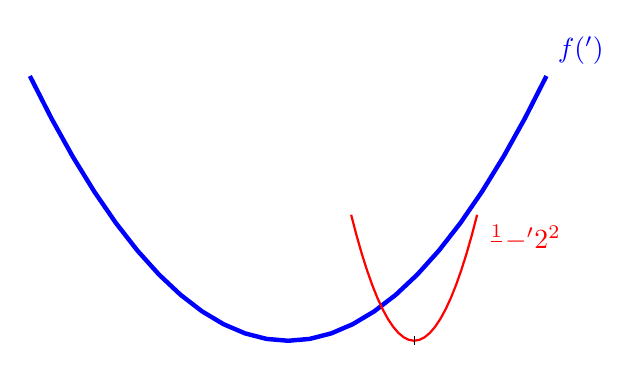
\begin{tikzpicture}[scale=0.8]
					% Original quadratic function
					\draw[blue, ultra thick, domain=-4.1:4.1] plot (\x, {(1/4)*\x*\x}) node[above right] {$f(\weights')$};		
					% Quadratic function with larger curvature, centered at w = 2
					\draw[red, thick, domain=1:3] plot (\x, {2*(\x - 2)*(\x - 2)}) node[below right] {$\frac{1}{\lrate}\normgeneric{\weights-\weights'}{2}^{2}$};
					% Axes
					% Minimum point of second curve
					\draw[shift={(2,0)}] (0pt,2pt) -- (0pt,-2pt) node[below] {$\weights$};
					%\node at (2,0.5) [anchor=north] {$\weights$};
				\end{tikzpicture}
			\end{center}
			\caption{The proximal operator updates a vector $\weights$ by minimizing a penalized version 
				of the \gls{function} $f(\cdot)$. The penalty term is the scaled squared Euclidean distance between the optimization 
				variable $\weights'$ and the given vector $\weights$.	\label{fig_proxoperator_opt_dict}}
		\end{figure}
		\foreignlanguage{greek}{Βλέπε επίσης:} \gls{convex}, \gls{function}, \gls{generalization}, \gls{gradstep}, \gls{smooth}, \gls{stepsize}.},
	first={\foreignlanguage{greek}{εγγύς τελεστής}},
	text={\foreignlanguage{greek}{εγγύς τελεστής}},
	user1={\foreignlanguage{greek}{εγγύς τελεστής}} %nominative
}

\newglossaryentry{bootstrap}
{name={\foreignlanguage{greek}{εκκίνηση}},
	description={\foreignlanguage{greek}{Για την ανάλυση μεθόδων}\index{\foreignlanguage{greek}{εκκίνηση}} 
		\glsentryuserii{ml}, \foreignlanguage{greek}{είναι συχνά χρήσιμο να ερμηνεύουμε ένα συγκεκριμένο σύνολο}  
		\glsentryuserv{datapoint} $\dataset = $ % 
		$\big\{ \datapoint^{(1)}, \ldots, \datapoint^{(\samplesize)}\big\}$ 
		\foreignlanguage{greek}{ως} \glsentryuservi{realization} \glsentryuserii{iid} \glsentryuserv{rv} 
		\foreignlanguage{greek}{που εξάγονται από μία κοινή} \glsentryuseriii{probdist} $p(\datapoint)$. 
		\foreignlanguage{greek}{Στην πράξη, η} \glsentryuseri{probdist} $p(\datapoint)$ \foreignlanguage{greek}{είναι 
		άγνωστη και πρέπει να εκτιμηθεί από το $\dataset$. Η προσέγγιση εκκίνησης χρησιμοποιεί το} 
		\glsentryuseriii{histogram} \foreignlanguage{greek}{του $\dataset$ ως μία εκτιμήτρια για την} $p(\datapoint)$. \\
		\foreignlanguage{greek}{Βλέπε επίσης:} \gls{ml}, \gls{datapoint}, \gls{realization}, \gls{iid}, \gls{rv}, \gls{probdist}, \gls{histogram}.},
	first={\foreignlanguage{greek}{εκκίνηση}},
	text={\foreignlanguage{greek}{εκκίνηση}},
	user1={\foreignlanguage{greek}{εκκίνηση}}, %nominative
	user2={\foreignlanguage{greek}{εκκίνησης}} %genitive  
}

\newglossaryentry{bayesestimator}
{name={\foreignlanguage{greek}{εκτιμήτρια} Bayes},
	description={\foreignlanguage{greek}{Θεωρούμε ένα}\index{\foreignlanguage{greek}{εκτιμήτρια} Bayes} 
		\glsentryuseriii{probmodel} \foreignlanguage{greek}{με μία από κοινού} \glsentryuseriii{probdist} $p(\featurevec,\truelabel)$ 
		\foreignlanguage{greek}{πάνω στα} \glsentryuservi{feature} $\featurevec$ \foreignlanguage{greek}{και την} \glsentryuseriii{label} 
		$\truelabel$ \foreignlanguage{greek}{ενός} \glsentryuserii{datapoint}. \foreignlanguage{greek}{Για μία δεδομένη} 
		\glsentryuseriii{lossfunc} $\lossfunc{\cdot}{\cdot}$, \foreignlanguage{greek}{αναφερόμαστε σε μία} \glsentryuseriii{hypothesis} 
		$\hypothesis$ \foreignlanguage{greek}{ως μία εκτιμήτρια} Bayes \foreignlanguage{greek}{αν η} \glsentryuseriv{risk} 
		\foreignlanguage{greek}{της $\expect\left\{\lossfunc{\pair{\featurevec}{\truelabel}}{\hypothesis}\right\}$ είναι η} 
		\glsentryuseriv{minimum} \foreignlanguage{greek}{επιτεύξιμη} \glsentryuseri{risk} \cite{LC}. \foreignlanguage{greek}{Σημείωση 
		ότι το αν μία} \glsentryuseri{hypothesis} \foreignlanguage{greek}{πληροί τις προϋποθέσεις για να θεωρηθεί εκτιμήτρια} Bayes 
		\foreignlanguage{greek}{εξαρτάται από την υποκείμενη} \glsentryuseriii{probdist} \foreignlanguage{greek}{και την επιλογή για 
		την} \glsentryuseriii{lossfunc} $\lossfunc{\cdot}{\cdot}$.\\
		\foreignlanguage{greek}{Βλέπε επίσης:} \gls{probmodel}, \gls{probdist}, \gls{feature}, \gls{label}, \gls{datapoint}, \gls{lossfunc}, 
		\gls{hypothesis}, \gls{risk}, \gls{minimum}.},
	first={\foreignlanguage{greek}{εκτιμήτρια} Bayes},
	text={\foreignlanguage{greek}{εκτιμήτρια} Bayes},
	user1={\foreignlanguage{greek}{εκτιμήτρια} Bayes}, %nominative
    	user2={\foreignlanguage{greek}{εκτιμήτριας} Bayes} %genitive
}

\newglossaryentry{minimum}
{name={\foreignlanguage{greek}{ελάχιστο}},
	description={\foreignlanguage{greek}{Δεδομένου ενός συνόλου πραγματικών αριθμών,}\index{\foreignlanguage{greek}{ελάχιστο}} 
		\foreignlanguage{greek}{το ελάχιστο είναι ο μικρότερος από αυτούς τους αριθμούς. Σημείωση ότι 
		για κάποια σύνολα, όπως το σύνολο αρνητικών πραγματικών αριθμών, το ελάχιστο δεν υφίσταται.} },
	first={\foreignlanguage{greek}{ελάχιστο}},
	text={\foreignlanguage{greek}{ελάχιστο}},
	user1={\foreignlanguage{greek}{ελάχιστο}}, %nominative
	user2={\foreignlanguage{greek}{ελάχιστου}}, %genitive 
	user3={\foreignlanguage{greek}{ελάχιστο}}, %accusativeoradj 
	user4={\foreignlanguage{greek}{ελάχιστη}} %nominativeoraccusativeadjfem 
}

\newglossaryentry{supremum}
{name={\foreignlanguage{greek}{ελάχιστο άνω φράγμα (ή} supremum)},
	description={The supremum\index{\foreignlanguage{greek}{ελάχιστο άνω φράγμα (ή} supremum)} 
		(supremum or least upper bound) of a set of real numbers is 
		the smallest number that is greater than or equal to every element in the set. More formally, a 
		real number $a$ is the supremum of a set $\mathcal{A} \subseteq \mathbb{R}$ if: 1) $a$ 
		is an upper bound of $\mathcal{A}$; and 2) no number smaller than $a$ is an upper bound of $\mathcal{A}$. 
		Every non-empty set of real numbers that is bounded above has a supremum, even if it does 
		not contain its supremum as an element \cite[Sec.~1.4]{RudinBookPrinciplesMatheAnalysis}.},
	first={\foreignlanguage{greek}{ελάχιστο άνω φράγμα (ή} supremum)},
	text={\foreignlanguage{greek}{ελάχιστο άνω φράγμα}},
	user1={\foreignlanguage{greek}{ελάχιστο άνω φράγμα}}, %nominative
    	user2={\foreignlanguage{greek}{ελάχιστου άνω φράγματος}}, %genitive 
    	user3={\foreignlanguage{greek}{ελάχιστο άνω φράγμα}} %accusative 
}

\newglossaryentry{erm}
{name={\foreignlanguage{greek}{ελαχιστοποίηση εμπειρικής διακινδύνευσης}}, 
	description={\foreignlanguage{greek}{Η ελαχιστοποίηση εμπειρικής διακινδύνευσης}\index{\foreignlanguage{greek}{ελαχιστοποίηση εμπειρικής διακινδύνευσης}} 
		(empirical risk minimization - ERM) \foreignlanguage{greek}{είναι το} \glsentryuseri{optproblem} \foreignlanguage{greek}{της  
		εύρεσης μίας} \glsentryuserii{hypothesis} \foreignlanguage{greek}{(από ένα} \glsentryuseriii{model}) \foreignlanguage{greek}{με 
		την} \glsentryuseriv{minimum} \foreignlanguage{greek}{μέση} \glsentryuseriii{loss} \foreignlanguage{greek}{(ή} \glsentryuseriii{emprisk}) 
		\foreignlanguage{greek}{σε ένα δεδομένο} \glsentryuseriii{dataset} 
		$\dataset$ \foreignlanguage{greek}{(δηλαδή το} \glsentryuseriii{trainset}). \foreignlanguage{greek}{Πολλές μέθοδοι} 
		\glsentryuserii{ml} \foreignlanguage{greek}{προκύπτουν από} \glsentryuseriii{emprisk} \foreignlanguage{greek}{μέσω 
		συγκεκριμένων επιλογών σχεδιασμού για το} \glsentryuseriii{dataset}, \foreignlanguage{greek}{το} \glsentryuseriii{model}, 
		\foreignlanguage{greek}{και την} \glsentryuseriii{loss} \cite[\foreignlanguage{greek}{Κεφ.} 3]{MLBasics}.\\
		\foreignlanguage{greek}{Βλέπε επίσης:} \gls{optproblem}, \gls{hypothesis}, \gls{model}, \gls{minimum}, \gls{loss}, \gls{emprisk}, \gls{dataset}, \gls{trainset}, \gls{ml}.},
	first={\foreignlanguage{greek}{ελαχιστοποίηση εμπειρικής διακινδύνευσης}},
	text={\foreignlanguage{greek}{ελαχιστοποίηση εμπειρικής διακινδύνευσης}},
	user1={\foreignlanguage{greek}{ελαχιστοποίηση εμπειρικής διακινδύνευσης}}, %nominative
	user2={\foreignlanguage{greek}{ελαχιστοποίησης εμπειρικής διακινδύνευσης}}, %genitive
	user3={\foreignlanguage{greek}{ελαχι\-στο\-ποί\-ηση εμπει\-ρι\-κής διακινδύνευσης}} %accusative 
}

\newglossaryentry{emprisk}
{name={\foreignlanguage{greek}{εμπειρική διακινδύνευση}},
  description={\foreignlanguage{greek}{Η εμπειρική} \glsentryuseri{risk}\index{\foreignlanguage{greek}{εμπειρική διακινδύνευση}} 
	$\emprisk{\hypothesis}{\dataset}$ \foreignlanguage{greek}{μίας} \glsentryuserii{hypothesis} \foreignlanguage{greek}{σε ένα} 
	\glsentryuseriii{dataset} $\dataset$ \foreignlanguage{greek}{είναι 
	η μέση} \glsentryuseri{loss} \foreignlanguage{greek}{που προκαλείται από την 
  	$\hypothesis$ όταν εφαρμόζεται στα} \glsentryuservi{datapoint} \foreignlanguage{greek}{του} $\dataset$.\\
	\foreignlanguage{greek}{Βλέπε επίσης:} \gls{risk}, \gls{hypothesis}, \gls{dataset}, \gls{loss}, \gls{datapoint}.},
  first={\foreignlanguage{greek}{εμπειρική διακινδύνευση}},
  text={empirical risk},
  user1={\foreignlanguage{greek}{εμπειρική διακινδύνευση}}, %nominative
  user2={\foreignlanguage{greek}{εμπειρικής διακινδύνευσης}}, %genitive 
  user3={\foreignlanguage{greek}{εμπειρική διακινδύνευση}} %accusative
}

\newglossaryentry{entropy}
{name={\foreignlanguage{greek}{εντροπία}},
	description={\foreignlanguage{greek}{Η εντροπία ποσοτικοποιεί την}\index{\foreignlanguage{greek}{εντροπία}} 
		\glsentryuseriii{uncertainty} \foreignlanguage{greek}{ή τη μη προβλεψιμότητα που σχετίζεται με μία} 
		\glsentryuseriii{rv} \cite{coverthomas}. 
		\foreignlanguage{greek}{Για μία διακριτή} \glsentryuseriii{rv} $x$ \foreignlanguage{greek}{που παίρνει 
		τιμές σε ένα πεπερασμένο σύνολο $\mathcal{S} = \{x_1, \ldots, x_n\}$ με μία} \glsentryuseriii{function}
		\foreignlanguage{greek}{μάζας} \glsentryuserii{probability} $p_i \defeq \prob{x = x_i}$, \foreignlanguage{greek}{η 
		εντροπία ορίζεται ως}
		\[
		H(x) \defeq -\sum_{i=1}^n p_i \log p_i.
		\]
		\foreignlanguage{greek}{Η εντροπία μεγιστοποιείται όταν όλα τα αποτελέσματα είναι εξίσου πιθανά, 
		και ελαχιστοποιείται (δηλαδή μηδενίζεται) όταν το αποτέλεσμα είναι ντετερμινιστικό. Η} 
		\glsentryuseri{generalization} \foreignlanguage{greek}{της έννοιας της εντροπίας για συνεχείς} 
		\glsentryuservi{rv} \foreignlanguage{greek}{είναι η} \glsentryuseri{diffentropy}. \\
		\foreignlanguage{greek}{Βλέπε επίσης:} \gls{uncertainty}, \gls{rv}, \gls{probability}, \gls{function}, \gls{generalization}, 
		\gls{diffentropy}, \gls{probmodel}.},
	first={\foreignlanguage{greek}{εντροπία}},
	text={\foreignlanguage{greek}{εντροπία}},
	user1={\foreignlanguage{greek}{εντροπία}}, %nominative
  	user2={\foreignlanguage{greek}{εντροπίας}} %genitive  
}

\newglossaryentry{explanation}
{name={\foreignlanguage{greek}{εξήγηση}},
	description={One approach to enhance the \gls{transparency} of an \gls{ml} method for its human user 
		is to provide an explanation\index{explanation} alongside the \gls{prediction}s delivered 
		by the method. Explanations can take different forms. For instance, they may 
        		consist of human-readable text or quantitative indicators, such as \gls{feature} 
        		importance scores for the individual \gls{feature}s of a given \gls{datapoint}~\cite{Molnar2019}. 
	   	Alternatively, explanations can be visual, for example, intensity \gls{map}s that highlight 
	   	image regions that drive the \gls{prediction} \cite{GradCamPaper}. 
       		Fig.\ \ref{fig_explanation_dict} illustrates two types of explanations. The first 
       		is a local linear approximation $g(\featurevec)$ of a non-linear trained \gls{model} 
       		$\learnthypothesis(\featurevec)$ around a specific \gls{featurevec} $\featurevec'$, 
       		as used in the method \gls{lime}. 
        		The second form of explanation depicted in the figure is a sparse set of \gls{prediction}s 
       		$\learnthypothesis(\featurevec^{(1)}), \learnthypothesis(\featurevec^{(2)}), \learnthypothesis(\featurevec^{(3)})$ 
       		at selected \gls{featurevec}s, offering concrete reference points for the user. 
	 	\begin{figure}[H]
	   		\begin{center}
	 		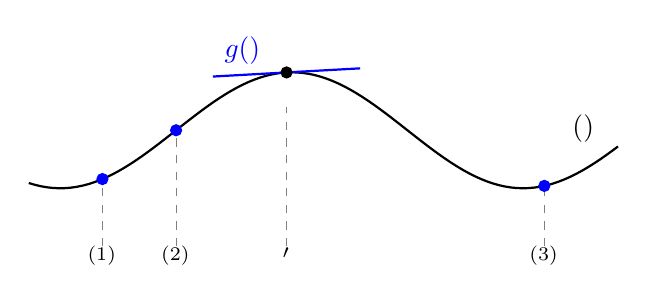
\begin{tikzpicture}[x=0.5cm]
	 		\begin{axis}[
	 			hide axis,
	 			xmin=-3, xmax=6,
	 			ymin=0, ymax=6,
	 			domain=0:6,
	 			samples=100,
	 			width=10cm,
	 			height=6cm,
	 			clip=false
	 		   ]
	 		% Original nonlinear function h(x)
			\addplot[thick, domain=-2:6] {2 + sin(deg(x))} 
	   		     node[pos=0.9, above right, yshift=10pt] {$\learnthypothesis(\featurevec)$};
	 		% Tangent line as local linear approximation at x = 1.5
	 		% h(3) = 2 + sin(3), h'(3) = cos(3)
	 		\addplot[blue, thick, domain=0.5:2.5] 
	 		{2 + sin(deg(1.5)) + cos(deg(1.5))*(x - 1.5)}
	 		node[pos=0.2, above] {$g(\featurevec)$};
	 		% Mark point of approximation
	 		\addplot[mark=*] coordinates {(1.5, {2 + sin(deg(1.5))})};
	 		    % Vertical dashed line (ruler) at x = 1.5
			\addplot[dashed, gray] coordinates {(1.5,0) (1.5,2.4)};
	 		\node at (axis cs:1.5, -0.2) {$\featurevec'$};
	      		% add function values for finite set of featurevecs
	       		\addplot[mark=*,blue] coordinates {(-1, {2 + sin(deg(-1))})};
	       		\addplot[dashed, gray] coordinates {(-1,0) (-1,{2 + sin(deg(-1))})};
	       		\node at (axis cs:-1, -0.2) {$\featurevec^{(1)}$};
	 	   	\addplot[mark=*,blue] coordinates {(0, {2 + sin(deg(0))})};
	 	   	\addplot[dashed, gray] coordinates {(0,0) (0,{2 + sin(deg(0))})};
	 	   	\node at (axis cs:0, -0.2) {$\featurevec^{(2)}$};
	 	   	\addplot[mark=*,blue] coordinates {(5, {2 + sin(deg(5))})};
	 	   	\addplot[dashed, gray] coordinates {(5,0) (5,{2 + sin(deg(5))})};
	 	   	\node at (axis cs:5, -0.2) {$\featurevec^{(3)}$};
	% 		    % Plot the two points
	% 		    % Coordinates of the two points
	% 		\pgfmathsetmacro{\xA}{-1.5}
	% 		\pgfmathsetmacro{\xB}{3}
	% 		\pgfmathsetmacro{\yA}{2 + sin(deg(\xA))}
	% 		\pgfmathsetmacro{\yB}{2 + sin(deg(\xB))}
	 		\end{axis}
	% 	\vspace*{-10mm}
		\end{tikzpicture}
	 	\end{center}
	 	\caption{A trained \gls{model} $\learnthypothesis(\featurevec)$ can be explained 
	     	locally at some point $\featurevec'$ by a linear approximation $g(\featurevec)$. 
	     	For a \gls{differentiable} $\learnthypothesis(\featurevec)$, this approximation is 
	     	determined by the \gls{gradient} $\nabla \learnthypothesis(\featurevec')$. Another 
	     	form of explanation could be the \gls{function} values $\learnthypothesis\big(\featurevec^{(\sampleidx)} \big)$ 
	     	for $\sampleidx=1,2,3$. 
		\label{fig_explanation_dict}}
	 	\end{figure} 
		\foreignlanguage{greek}{Βλέπε επίσης:} \gls{transparency}, \gls{ml}, \gls{prediction}, \gls{feature}, \gls{datapoint}, 
		\gls{map}, \gls{model}, \gls{featurevec}, \gls{lime}, \gls{differentiable}, \gls{gradient}, \gls{function}, \gls{classification}.},
	first={\foreignlanguage{greek}{εξήγηση}},
	text={\foreignlanguage{greek}{εξήγηση}},
	user1={\foreignlanguage{greek}{εξήγηση}}, %nominative
    	user2={\foreignlanguage{greek}{εξήγησης}}, %genitive  
	user3={\foreignlanguage{greek}{εξήγηση}}, %accusative
    	user4={\foreignlanguage{greek}{εξηγήσεις}}, %nominativepl  
	user5={\foreignlanguage{greek}{εξηγήσεων}}, %genitivepl
    	user6={\foreignlanguage{greek}{εξηγήσεις}} %accusativepl  
}

\newglossaryentry{eerm}
{name={\foreignlanguage{greek}{εξηγήσιμη ελαχιστοποίηση εμπειρικής διακινδύνευσης}}, 
	description={EERM (explainable empirical risk minimization - EERM) is 
		an\index{\foreignlanguage{greek}{εξηγήσιμη ελαχιστοποίηση εμπειρικής διακινδύνευσης}} 
		instance of \gls{srm} that adds a \gls{regularization} term to the average \gls{loss} in the \gls{objfunc} of \gls{erm}. 
		The \gls{regularization} term is chosen to favor \gls{hypothesis} \gls{map}s that are intrinsically 
		explainable for a specific user. This user is characterized by their \gls{prediction}s provided 
		for the \gls{datapoint}s in a \gls{trainset} \cite{Zhang:2024aa}.\\
		\foreignlanguage{greek}{Βλέπε επίσης:} \gls{srm}, \gls{regularization}, \gls{loss}, \gls{objfunc}, \gls{erm}, \gls{hypothesis}, 
		\gls{map}, \gls{prediction}, \gls{datapoint}, \gls{trainset}.},
	first={\foreignlanguage{greek}{εξηγήσιμη ελαχιστοποίηση εμπειρικής διακινδύνευσης}}, 
	text={\foreignlanguage{greek}{εξηγήσιμη ελαχιστοποίηση εμπειρικής διακινδύνευσης}},
	user1={\foreignlanguage{greek}{εξηγήσιμη ελαχιστοποίηση εμπειρικής διακινδύνευσης}}, %nominative
  	user2={\foreignlanguage{greek}{εξηγήσιμης ελαχιστοποίησης εμπειρικής διακινδύνευσης}} %genitive 
}

\newglossaryentry{xml}
{name={\foreignlanguage{greek}{εξηγήσιμη μηχανική μάθηση}}, 
	description={XML\index{\foreignlanguage{greek}{εξηγήσιμη μηχανική μάθηση}} (explainable machine learning - XML)
		methods aim to complement each \gls{prediction} with an \gls{explanation} of 
		how the \gls{prediction} has been obtained. The construction of an explicit \gls{explanation} 
		might not be necessary if the \gls{ml} method uses a sufficiently simple (or interpretable) \gls{model} \cite{rudin2019stop}.\\
		\foreignlanguage{greek}{Βλέπε επίσης:} \gls{prediction}, \gls{explanation}, \gls{ml}, \gls{model}.},
	first={\foreignlanguage{greek}{εξηγήσιμη μηχανική μάθηση}},
	text={\foreignlanguage{greek}{εξηγήσιμη μηχανική μάθηση}},
	user1={\foreignlanguage{greek}{εξηγήσιμη μηχανική μάθηση}}, %nominative
  	user2={\foreignlanguage{greek}{εξηγήσιμη μηχανική μάθηση}} %genitive  
}

\newglossaryentry{explainability}
{name={\foreignlanguage{greek}{εξηγησιμότητα}},
	description={\foreignlanguage{greek}{Ορίζουμε την (υποκειμενική) εξηγησιμότητα μίας μεθόδου}\index{\foreignlanguage{greek}{εξηγησιμότητα}} 
		\glsentryuserii{ml} \foreignlanguage{greek}{ως το επίπεδο προσομοιωσιμότητας} \cite{Colin:2022aa} \foreignlanguage{greek}{των} 
		\glsentryuserv{prediction} \foreignlanguage{greek}{που παραδίδονται από ένα σύστημα} \glsentryuserii{ml} \foreignlanguage{greek}{σε 
		έναν χρήστη που είναι άνθρωπος. Ποσοτικά μέτρα για την (υποκειμενική) εξηγησιμότητα ενός εκπαιδευμένου} 
		\glsentryuserii{model} \foreignlanguage{greek}{μπορούν να κατασκευαστούν συγκρίνοντας τις}  
		\glsentryuservi{prediction} \foreignlanguage{greek}{του με τις} \glsentryuservi{prediction} \foreignlanguage{greek}{που 
		παρέχονται από έναν χρήστη σε ένα} \glsentryuseriii{testset} \cite{Colin:2022aa}, \cite{Zhang:2024aa}. 
		\foreignlanguage{greek}{Εναλλακτικά, μπορούμε να χρησιμοποιήσουμε} \glsentryuservi{probmodel} 
		\foreignlanguage{greek}{για} \glsentryuseriii{data} \foreignlanguage{greek}{και να μετρήσουμε την εξηγησιμότητα ενός εκπαιδευμένου}  
		\glsentryuserii{model} \glsentryuserii{ml} \foreignlanguage{greek}{μέσω της υπό συνθήκης (διαφορικής)} \glsentryuserii{entropy} 
		\foreignlanguage{greek}{των} \glsentryuservii{prediction} \foreignlanguage{greek}{του}, \foreignlanguage{greek}{δεδομένων των} 
		\glsentryuserv{prediction} \foreignlanguage{greek}{του χρήστη} \cite{JunXML2020}, \cite{Chen2018}. \\
		\foreignlanguage{greek}{Βλέπε επίσης:} \gls{ml}, \gls{prediction}, \gls{model}, \gls{testset}, \gls{probmodel}, \gls{data}, \gls{entropy}, \gls{trustAI}, \gls{regularization}. },
	first={\foreignlanguage{greek}{εξηγησιμότητα}},
	text={\foreignlanguage{greek}{εξηγησιμότητα}},
	user1={\foreignlanguage{greek}{εξηγησιμότητα}}, %nominative
	user2={\foreignlanguage{greek}{εξηγησιμότητας}}, %genitive 
	user3={\foreignlanguage{greek}{εξηγησιμότητα}} %accusative
}

\newglossaryentry{dataaug}
{name={\foreignlanguage{greek}{επαύξηση δεδομένων}},
	description={\Gls{data} augmentation\index{\foreignlanguage{greek}{επαύξηση δεδομένων}} 
		methods add synthetic \gls{datapoint}s 
		to an existing set of \gls{datapoint}s. These synthetic \gls{datapoint}s are obtained by 
		perturbations (e.g., adding noise to physical measurements) or transformations 
		(e.g., rotations of images) of the original \gls{datapoint}s. These perturbations and 
		transformations are such that the resulting synthetic \gls{datapoint}s should 
		still have the same \gls{label}. As a case in point, a rotated cat image is still 
		a cat image even if their \gls{featurevec}s (obtained by stacking pixel color intensities) 
		are very different (see Fig. \ref{fig_symmetry_dataaug_dict}). \Gls{data} augmentation can be an 
		efficient form of \gls{regularization}.
		\begin{figure}[H]
		\begin{center}
			\begin{tikzpicture}
				% Define shift macros locally
				\newcommand{\xshift}{0.5}
				\newcommand{\yshift}{2}
				% Define the shifted curves
				% Define the shifted curves
  				\draw[very thick, blue] plot[smooth, tension=1] coordinates {(0,0) (2,1) (4,0) (6,-1) (8,0)};
  				\node[blue, right] at (0,0) {\textbf{cat}};
  				\draw[very thick, red, dashed] plot[smooth, tension=1] coordinates {(0 + \xshift,0 + \yshift) (2 + \xshift,1 + \yshift) (4 + \xshift,0 + \yshift) (6 + \xshift,-1 + \yshift) (8 + \xshift,0 + \yshift)};
  				\node[red, right] at (8 + \xshift,0 + \yshift) {\textbf{no cat}};
				\fill[blue] (2,1) circle (2pt) node[above] {$\featurevec^{(1)}$};
				\fill[blue] (6,-1) circle (2pt) node[above] {$\featurevec^{(2)}$};
				  % Draw a bent arrow connecting the two points with custom in and out angles
				  \draw[->, thin, >=latex, line width=0.5pt] (2,1) to[out=240, in=240] node[midway, below] {$\mathcal{T}^{(\eta)}$} (6,-1);
			  \end{tikzpicture}
			  \vspace*{-11mm}
		\end{center}
		\caption{\Gls{data} augmentation exploits intrinsic symmetries of \gls{datapoint}s in 
		some \gls{featurespace} $\featurespace$. We can represent a symmetry by 
		an operator $\mathcal{T}^{(\eta)}: \featurespace \rightarrow \featurespace$,
		parametrized by some number $\eta \in \mathbb{R}$. For example, $\mathcal{T}^{(\eta)}$ 
		might represent the effect of rotating a cat image by $\eta$ degrees. A \gls{datapoint} 
		with \gls{featurevec} $\featurevec^{(2)} = \mathcal{T}^{(\eta)} \big(\featurevec^{(1)} \big)$ must 
		have the same \gls{label} $\truelabel^{(2)}=\truelabel^{(1)}$ as a \gls{datapoint} 
		with \gls{featurevec} $\featurevec^{(1)}$.\label{fig_symmetry_dataaug_dict}}
		\end{figure} 
		\foreignlanguage{greek}{Βλέπε επίσης:} \gls{data}, \gls{datapoint}, \gls{label}, \gls{featurevec}, \gls{regularization}, \gls{featurespace}. },
	first={data augmentation},
	text={data augmentation},
	user1={\foreignlanguage{greek}{επαύξηση δεδομένων}}, %nominative
  	user2={\foreignlanguage{greek}{επαύξησης δεδομένων}} %genitive 
}

\newglossaryentry{attack}
{name={\foreignlanguage{greek}{επίθεση}},
	description={\foreignlanguage{greek}{Μία επίθεση σε ένα σύστημα}\index{\foreignlanguage{greek}{επίθεση}} \glsentryuserii{ml} 
		\foreignlanguage{greek}{αναφέρεται σε μία σκόπιμη ενέργεια—είτε ενεργή είτε παθητική—που διακυβεύει την ακεραιότητα,
		τη διαθεσιμότητα, ή την εμπιστευτικότητα του συστήματος. Οι ενεργές επιθέσεις περιλαμβάνουν τη διαταραχή 
		συνιστωσών όπως των} \glsentryuserv{dataset} (\foreignlanguage{greek}{μέσω} \gls{datapoisoning}) 
		\foreignlanguage{greek}{ή τους συνδέσμους επικοινωνίας μεταξύ} \glsentryuserv{device} \foreignlanguage{greek}{εντός μίας 
		εφαρμογής} \glsentryuserii{ml}. \foreignlanguage{greek}{Οι παθητικές επιθέσεις, όπως οι} \glsentryuseriv{privattack}, 
		\foreignlanguage{greek}{στοχεύουν να συμπεράνουν} \glsentryuservi{sensattr} \foreignlanguage{greek}{χωρίς να τροποποιήσουν 
		το σύστημα. Ανάλογα με τον στόχο τους, μπορούμε να διακρίνουμε ανάμεσα σε} \glsentryuservi{dosattack}, 
		\foreignlanguage{greek}{επιθέσεις} \glsentryuserii{backdoor}, \foreignlanguage{greek}{και} \glsentryuservi{privattack}.\\
		\foreignlanguage{greek}{Βλέπε επίσης:} \gls{ml}, \gls{dataset}, \gls{datapoisoning}, \gls{device}, \gls{privattack}, 
		\gls{sensattr}, \gls{dosattack}, \gls{backdoor}.},
	first={\foreignlanguage{greek}{επίθεση}},
	text={\foreignlanguage{greek}{επίθεση}},
	user1={\foreignlanguage{greek}{επίθεση}}, %nominative
  	user2={\foreignlanguage{greek}{επίθεσης}} %genitive 
}

\newglossaryentry{dosattack}
{name={\foreignlanguage{greek}{επίθεση άρνησης υπηρεσιών}}, 
	description={\foreignlanguage{greek}{Μία}\index{\foreignlanguage{greek}{επίθεση άρνησης υπηρεσιών}} 
		\glsentryuseri{attack} \foreignlanguage{greek}{άρνησης υπηρεσιών στοχεύει (π.χ. μέσω} \gls{datapoisoning}) 
		\foreignlanguage{greek}{να κατευθύνει την εκπαίδευση ενός} \glsentryuserii{model}, 
		\foreignlanguage{greek}{έτσι ώστε να έχει χαμηλή επίδοση για τυπικά} \glsentryuservi{datapoint}.\\
		\foreignlanguage{greek}{Βλέπε επίσης:} \gls{attack}, \gls{datapoisoning}, \gls{model}, \gls{datapoint}.},
	first={\foreignlanguage{greek}{επίθεση άρνησης υπηρεσιών}},
	text={\foreignlanguage{greek}{επίθεση άρνησης υπηρεσιών}},
	user1={\foreignlanguage{greek}{επίθεση άρνησης υπηρεσιών}}, %nominative
  	user2={\foreignlanguage{greek}{επίθεσης άρνησης υπηρεσιών}}, %genitive 
	user3={\foreignlanguage{greek}{επίθεση άρνησης υπηρεσιών}}, %accusative
  	user4={\foreignlanguage{greek}{επιθέσεις άρνησης υπηρεσιών}}, %nominativepl 
	user5={\foreignlanguage{greek}{επιθέσεων άρνησης υπηρεσιών}}, %genitivepl
  	user6={\foreignlanguage{greek}{επιθέσεις άρνησης υπηρεσιών}} %accusativepl 
}

\newglossaryentry{privattack}
{name={\foreignlanguage{greek}{επίθεση της ιδιωτικότητας}},
	description={\foreignlanguage{greek}{Μία} \glsentryuseri{attack}\index{\foreignlanguage{greek}{επίθεση της ιδιωτικότητας}} 
		\foreignlanguage{greek}{της ιδιωτικότητας σε ένα σύστημα} \glsentryuserii{ml} \foreignlanguage{greek}{στοχεύει 
		να συμπεράνει} \glsentryuservi{sensattr} \foreignlanguage{greek}{ατόμων εκμεταλλευόμενη μερική πρόσβαση σε 
		ένα εκπαιδευμένο} \glsentryuseriii{model} \glsentryuserii{ml}. \foreignlanguage{greek}{Μία μορφή} \glsentryuserii{attack} 
		\foreignlanguage{greek}{της ιδιωτικότητας εί\-ναι η} \gls{modelinversion}.\\
		\foreignlanguage{greek}{Βλέπε επίσης:} \gls{attack}, \gls{ml}, \gls{sensattr}, \gls{model}, \gls{modelinversion}, \gls{trustAI}, \gls{gdpr}.},
	first={\foreignlanguage{greek}{επίθεση της ιδιωτικότητας}},
	text={\foreignlanguage{greek}{επίθεση της ιδιωτικότητας}},
	user1={\foreignlanguage{greek}{επίθεση της ιδιωτικότητας}}, %nominative
  	user2={\foreignlanguage{greek}{επίθεσης της ιδιωτικότητας}}, %genitive 
	user3={\foreignlanguage{greek}{επίθεση της ιδιωτικότητας}}, %accusative
  	user4={\foreignlanguage{greek}{επιθέσεις της ιδιωτικότητας}}, %nominativepl 
	user5={\foreignlanguage{greek}{επιθέσεων της ιδιωτικότητας}}, %genitivepl 
	user6={\foreignlanguage{greek}{επιθέσεις της ιδιωτικότητας}}, %accusativepl
}

\newglossaryentry{validation} 
{name={\foreignlanguage{greek}{επικύρωση}},
	description={\foreignlanguage{greek}{Θεωρούμε μία}\index{\foreignlanguage{greek}{επικύρωση}} 
		\glsentryuseri{hypothesis} $\learnthypothesis$ 
		\foreignlanguage{greek}{που έχει μαθευτεί μέσω κάποιας μεθόδου} \glsentryuserii{ml}, \foreignlanguage{greek}{π.χ. λύνοντας την} 
		\glsentryuseriii{erm} \foreignlanguage{greek}{σε ένα} \glsentryuseriii{trainset} $\dataset$. 
		\foreignlanguage{greek}{Η επικύρωση αναφέρεται στην πρακτική της αξιολόγησης της} \glsentryuserii{loss} 
		\foreignlanguage{greek}{που προκαλείται από την} \glsentryuseriii{hypothesis} $\learnthypothesis$ \foreignlanguage{greek}{σε ένα 
		σύνολο} \glsentryuserv{datapoint} \foreignlanguage{greek}{που δεν περιέχονται στο} \glsentryuseriii{trainset} $\dataset$.\\
		\foreignlanguage{greek}{Βλέπε επίσης:} \gls{hypothesis}, \gls{ml}, \gls{erm}, \gls{trainset}, \gls{loss}, \gls{datapoint}.},
	first={\foreignlanguage{greek}{επικύρωση}},
	text={\foreignlanguage{greek}{επικύρωση}},
	user1={\foreignlanguage{greek}{επικύρωση}}, %nominative
	user2={\foreignlanguage{greek}{επικύρωσης}}, %genitive
	user3={\foreignlanguage{greek}{επικύρωση}} %accusative  
}

\newglossaryentry{modelsel}
{name={\foreignlanguage{greek}{επιλογή μοντέλου}},
	description={In\index{\foreignlanguage{greek}{επιλογή μοντέλου}} \gls{ml}, \gls{model} selection refers to the 
		process of choosing between different candidate \gls{model}s. In its most 
		basic form, \gls{model} selection amounts to: 1) training each candidate \gls{model}; 
		2) computing the \gls{valerr} for each trained \gls{model}; and 3) choosing the \gls{model} 
		with the smallest \gls{valerr} \cite[Ch. 6]{MLBasics}.\\
		\foreignlanguage{greek}{Βλέπε επίσης:} \gls{ml}, \gls{model}, \gls{valerr}. },
	first={\foreignlanguage{greek}{επιλογή μοντέλου}},
	text={\foreignlanguage{greek}{επιλογή μοντέλου}},
	user1={\foreignlanguage{greek}{επιλογή μοντέλου}}, %nominative
	user2={\foreignlanguage{greek}{επιλογής μοντέλου}} %genitive
}

\newglossaryentry{learningtask}
{name={\foreignlanguage{greek}{εργασία μάθησης}},
	description={Consider\index{\foreignlanguage{greek}{εργασία μάθησης}} a \gls{dataset} $\dataset$ consisting of 
%		multiple \gls{datapoint}s $\datapoint^{(1)},\ldots,\datapoint^{(\samplesize)}$. 
%		For example, $\dataset$ might represent a collection of images in an image database. 
%		A learning task is defined by specifying those properties (or attributes) of a \gls{datapoint} 
%		that are used as its \gls{feature}s and \gls{label}s. Given a choice of \gls{model} $\hypospace$ and 
%		\gls{lossfunc}, a learning task leads to an instance of \gls{erm} and can thus be 
%		represented by the associated \gls{objfunc} $\emprisk{\hypothesis}{\dataset}$ for $\hypothesis \in \hypospace$. 
%		Importantly, multiple distinct learning tasks can be constructed from the same \gls{dataset} 
%		by selecting different sets of \gls{feature}s and \gls{label}s. 
%    		\begin{figure}[H]
%			\centering
%			% Top row: image
%			\begin{minipage}[t]{0.95\textwidth}
%    			\centering
%    			\includegraphics[width=\textwidth]{assets/CowsAustria.jpg}
%    			\caption*{An image showing cows grazing in the Austrian countryside.}
%			\vspace{5mm}
%			\end{minipage}
%			\vspace{5mm}
%			% Bottom row: two learning tasks
%			\begin{minipage}[t]{0.45\textwidth}
%    			Task 1 (\gls{regression}):
%    			\begin{itemize}
%        			\item \Gls{feature}s: The RGB values of all image pixels.
%        			\item \Gls{label}: The number of cows depicted.
%    			\end{itemize}
%			\end{minipage}
%			\hfill
%			\begin{minipage}[t]{0.45\textwidth}
%    			Task 2 (\gls{classification}):
%    			\begin{itemize}
%        			\item \Gls{feature}s: The average green intensity of the image.
%        			\item \Gls{label}: Should cows be moved to another location (yes/no)?
%    			\end{itemize}
%			\end{minipage}
%			\caption{Two learning tasks constructed from a single image \gls{dataset}. 
%			These tasks differ in \gls{feature} selection and choice of \gls{label} (i.e., the objective), 
%			but are both derived from the same \gls{dataset}.}
%			\label{fig:learning_tasks_cows_dict}
%		\end{figure}
%		Such tasks are inherently related, and solving them jointly, e.g., using \gls{multitask learning} 
%		methods, is often more effective than treating them independently 
%		\cite{Caruana:1997wk}, \cite{JungGaphLassoSPL}, \cite{CSGraphSelJournal}.
		\\
	 	\foreignlanguage{greek}{Βλέπε επίσης:} \gls{dataset}, \gls{datapoint}, \gls{feature}, \gls{label}, \gls{model}, 
		\gls{lossfunc}, \gls{erm}, \gls{objfunc}, \gls{regression}, \gls{classification}, \gls{multitask learning}, \gls{labelspace}.},
	first={\foreignlanguage{greek}{εργασία μάθησης}},
	text={\foreignlanguage{greek}{εργασία μάθησης}},
	user1={\foreignlanguage{greek}{εργασία μάθησης}}, %nominative
	user2={\foreignlanguage{greek}{εργασίας μάθησης}}, %genitive 
	user3={\foreignlanguage{greek}{εργασία μάθησης}}, %accusative
	user4={\foreignlanguage{greek}{εργασίες μάθησης}}, %nominativepl 
	user5={\foreignlanguage{greek}{εργασιών μάθησης}}, %genitivepl
	user6={\foreignlanguage{greek}{εργασίες μάθησης}} %accusativepl 
}

\newglossaryentry{interpretability}
{name={\foreignlanguage{greek}{ερμηνευσιμότητα}},
	description={\foreignlanguage{greek}{Μία μέθοδος} \glsentryuserii{ml}\index{\foreignlanguage{greek}{ερμηνευσιμότητα}}
		\foreignlanguage{greek}{είναι ερμηνεύσιμη για έναν χρήστη που είναι άνθρωπος αν μπορεί να κατανοήσει  
 		τη διαδικασία απόφασης της μεθόδου. Μία προσέγγιση για την ανάπτυξη ενός ακριβούς ορισμού της 
		ερμηνευσιμότητας είναι μέσω της έννοιας της προσομοιωσιμότητας, δηλαδή τη δυνατότητα ενός ανθρώπου να 
		προσομοιώνει διανοητικά τη συμπεριφορά του} \glsentryuserii{model}  
		\cite{Colin:2022aa}, \cite{Chen2018}, \cite{doshi2017towards}, \cite{hase-bansal-2020-evaluating}, \cite{Lipton2018}. 
 		\foreignlanguage{greek}{Αυτή η ιδέα έχει ως εξής: Αν ένας χρήστης που είναι άνθρωπος καταλαβαίνει μία μέθοδο} 
		\glsentryuserii{ml}, \foreignlanguage{greek}{τότε θα πρέπει να έχει τη δυνατότητα να αναμένει τις} \glsentryuservi{prediction}
 		\foreignlanguage{greek}{της σε ένα} \glsentryuseriii{testset}. \foreignlanguage{greek}{Παρουσιάζουμε ένα τέτοιο}  
 		\glsentryuseriii{testset} \foreignlanguage{greek}{στο Σχ.} \ref{fig_aug_simulatability_dict}, \foreignlanguage{greek}{το οποίο 
		επίσης απεικονίζει δύο} \glsentryuservi{hypothesis} $\learnthypothesis$ \foreignlanguage{greek}{και} $\learnthypothesis'$ 
		\foreignlanguage{greek}{που έχουν μαθευτεί. Η μέθοδος} \glsentryuserii{ml} \foreignlanguage{greek}{που παράγει την} 
		\glsentryuseriii{hypothesis} $\learnthypothesis$ \foreignlanguage{greek}{είναι ερμηνεύσιμη στον χρήστη που είναι άνθρωπος 
		και εξοικειωμένος με την έννοια της} \gls{linearmap}. \foreignlanguage{greek}{Εφόσον η $\learnthypothesis$ αντιστοιχεί 
		σε μία} \gls{linearmap}, \foreignlanguage{greek}{ο χρήστης μπορεί να αναμένει τις} \glsentryuservi{prediction} 
		\foreignlanguage{greek}{της $\learnthypothesis$ στο} \glsentryuseriii{testset}. \foreignlanguage{greek}{Αντίθετα, η 
		μέθοδος} \glsentryuserii{ml} \foreignlanguage{greek}{που παραδίδει την $\learnthypothesis'$ δεν είναι ερμηνεύσιμη, 
		επειδή η συμπεριφορά της δεν συμβαδίζει πλέον με τις} \glsentryuservi{expectation} \foreignlanguage{greek}{του χρήστη}.
 		\begin{figure}[H]
 			\begin{center} 
			\begin{tikzpicture}[x=1.5cm, y=1cm]
  			% Adjustable parameters
 			\def\slope{0.4}
  			\def\offset{2.0}
  			% Axes
  			\draw[->, very thick] (0,0.5) -- (7.7,0.5) node[below, xshift=-1cm] {$\feature$}; % x-axis
 			\draw[->, very thick] (0.5,0) -- (0.5,4.2) node[above] {$\truelabel$};           % y-axis
  			% Model line
  			\draw[color=black, thick, dashed, domain=-0.5:7.2, variable=\x] 
    			plot ({\x},{\slope*\x + \offset});
			% non-interpretable model
  			\draw[color=black, thick, dashed, domain=4:7.2, variable=\x] 
    			plot ({\x},{\slope*\x + \offset-(\x-4)*0.5});
  			\node[above] at (7.2, {\slope*7.2 + \offset}) {$\learnthypothesis(\feature)$};
  			\node[above] at (7.2, {\slope*7.2 + \offset - 0.5*(7.2 - 4)}) {$\learnthypothesis'(\feature)$};
 			%\node[above] at (7.2, {\slope*7.2 + \offset-(7.2-4)*0.3}) {$\learnthypothesis'(\feature)$};
  			% Training Data points
  			\foreach \x/\y/\c/\s in {
      			1.2/1.0/blue/6, 1.4/1.0/blue/6, 1.7/1.0/blue/6,
      			2.2/3.9/blue/12, 2.6/4.2/blue/12, 3.0/4.4/blue/12
  			}{
    			\coordinate (pt) at (\x,\y);
    			\node[fill=\c, circle, draw, minimum size=\s pt, scale=0.6] at (pt) {};
    			\draw[<->, >={Latex[width=2mm,length=4mm]}, color=\c, thick]
      			(\x, {\slope*\x + \offset}) -- (pt);
  			}
  			% test set with pseudo-labels
    			\foreach \x/\y/\c/\s in {
       			5.7/2.6/red/12, 5.9/2.6/red/12, 6.2/2.6/red/12
   			}{
     			\coordinate (pt) at (\x,{\slope*\x + \offset});
     			\node[fill=\c, circle, draw, minimum size=\s pt, scale=0.6] at (pt) {};
   			}
  			% Legend
  			\draw[fill=blue] (4.2, 1.7) circle (0.1cm) node [black,xshift=0.2cm,anchor=west] {\gls{trainset} $\dataset$};
  			\draw[fill=red]  (4.2, 1.2) circle (0.1cm) node [black,xshift=0.2cm,anchor=west] {\gls{testset} $\dataset'$};
			\end{tikzpicture}
			{\selectlanguage{greek}
 			\caption{\foreignlanguage{greek}{Μπορούμε να αξιολογήσουμε την ερμηνευσιμότητα εκπαιδευμένων} \glsentryuserv{model}  
 			$\learnthypothesis$ \foreignlanguage{greek}{και $\learnthypothesis'$ συγκρίνοντας τις} \glsentryuservi{prediction} 
			\foreignlanguage{greek}{τους με τις ψευδο-}\glsentryuservi{label} \foreignlanguage{greek}{που παράγονται από έναν 
			χρήστη που είναι άνθρωπος για το} $\dataset'$. 
			\label{fig_aug_simulatability_dict}} }
 			\end{center}
	 	\end{figure} 
 	 	\foreignlanguage{greek}{Η έννοια της ερμηνευσιμότητας σχετίζεται στενά με την έννοια της} \glsentryuserii{explainability}, 
 	 	\foreignlanguage{greek}{καθώς και οι δύο στοχεύουν να κάνουν τις μεθόδους} \glsentryuserii{ml} \foreignlanguage{greek}{πιο 
		κατανοητές στους ανθρώπους. Στο πλάισιο του Σχ.} \ref{fig_aug_simulatability_dict}, \foreignlanguage{greek}{η 
		ερμηνευσιμότητα μίας μεθόδου} \glsentryuserii{ml} $\learnthypothesis$ \foreignlanguage{greek}{απαιτεί ο χρήστης που είναι 
		άνθρωπος να μπορεί να αναμένει τις} \glsentryuservi{prediction} \foreignlanguage{greek}{της σε ένα αυθαίρετο} 
	 	\glsentryuseriii{testset}. \foreignlanguage{greek}{Αυτό ξεχωρίζει σε σχέση με την} \glsentryuseriii{explainability}, 
		\foreignlanguage{greek}{όπου ο χρήστης υποστηρίζεται από εξωτερικές} \glsentryuservi{explanation}—\foreignlanguage{greek}{όπως}  
		\gls{map}s \foreignlanguage{greek}{υπεροχής ή παραδείγματα αναφοράς από το} \glsentryuseriii{trainset}—\foreignlanguage{greek}{για 
		να καταλάβει τις} \glsentryuservi{prediction} \foreignlanguage{greek}{της $\learnthypothesis$ σε ένα συγκεκριμένο} 
		\glsentryuseriii{testset} $\dataset'$. \\ 
	 	\foreignlanguage{greek}{Βλέπε επίσης:} \gls{ml}, \gls{model},\gls{prediction}, \gls{testset}, \gls{hypothesis}, \gls{linearmap}, \gls{expectation}, 
		\gls{trainset}, \gls{label}, \gls{explainability}, \gls{explanation}, \gls{map}, \gls{trustAI}, \gls{regularization}, \gls{lime}.},
	first={\foreignlanguage{greek}{ερμηνευσιμότητα}},
	text={\foreignlanguage{greek}{ερμηνευσιμότητα}},
	user1={\foreignlanguage{greek}{ερμηνευσιμότητα}}, %nominative
	user2={\foreignlanguage{greek}{ερμηνευσιμότητας}} %genitive 
}

\newglossaryentry{label}
{name={\foreignlanguage{greek}{ετικέτα}},
	description={\foreignlanguage{greek}{Ένα υψηλότερου επιπέδου γεγονός ή ποσότητα ενδιαφέροντος}\index{\foreignlanguage{greek}{ετικέτα}} 
		\foreignlanguage{greek}{που σχετίζεται με ένα} \glsentryuseriii{datapoint}. \foreignlanguage{greek}{Για παράδειγμα, αν ένα} \glsentryuseri{datapoint} 
		\foreignlanguage{greek}{είναι μία εικόνα, η ετικέτα θα μπορούσε να υποδεικνύει αν η εικόνα περιέχει μία γάτα ή όχι. 
		Συνώνυμα του όρου ετικέτα, που χρησιμοποι\-ού\-νται συχνά σε συγκεκριμένους τομείς, περιλαμβάνουν 
		\guillemotleft μεταβλητή απόκρισης,\guillemotright\ \guillemotleft μεταβλητή εξόδου,\guillemotright\ και \guillemotleft στόχος\guillemotright} 
		\cite{Gujarati2021}, \cite{Dodge2003}, \cite{Everitt2022}.\\
		\foreignlanguage{greek}{Βλέπε επίσης:} \gls{datapoint}. },
	first={\foreignlanguage{greek}{ετικέτα}},
	text={\foreignlanguage{greek}{ετικέτα}},
	user1={\foreignlanguage{greek}{ετικέτα}}, %nominative
  	user2={\foreignlanguage{greek}{ετικέτας}}, %genitive 
	user3={\foreignlanguage{greek}{ετικέτα}}, %accusative
	user4={\foreignlanguage{greek}{ετικέτες}}, %nominativepl
  	user5={\foreignlanguage{greek}{ετικετών}}, %genitivepl 
	user6={\foreignlanguage{greek}{ετικέτες}} %accusativepl       
}

\newglossaryentry{sensattr}
{name={\foreignlanguage{greek}{ευαίσθητο ιδιοχαρακτηριστικό}},
	description={\foreignlanguage{greek}{Η} \glsentryuseri{ml}\index{\foreignlanguage{greek}{ευαίσθητο ιδιοχαρακτηριστικό}} 
		\foreignlanguage{greek}{περιστρέφεται γύρω από τη μάθηση μίας} \gls{map} \glsentryuserii{hypothesis} 
		\foreignlanguage{greek}{που μας επιτρέπει να προβλέψουμε την} \glsentryuseriii{label} \foreignlanguage{greek}{ενός} 
		\glsentryuserii{datapoint} \foreignlanguage{greek}{από τα} \glsentryuservi{feature} \foreignlanguage{greek}{του}. 
		\foreignlanguage{greek}{Σε κάποιες εφαρμογές, πρέπει να εξασφαλίσουμε ότι η έξοδος που παραδίδεται 
		από ένα σύστημα} \glsentryuserii{ml} \foreignlanguage{greek}{δεν μας επιτρέπει να συμπεράνουμε 
		ευαί\-σθητα ιδιοχαρακτηριστικά ενός} \glsentryuserii{datapoint}. \foreignlanguage{greek}{Ποιο μέρος  
		ενός} \glsentryuserii{datapoint} \foreignlanguage{greek}{θεωρείται ευαίσθητο ιδιοχαρακτηριστικό είναι μία 
		επιλογή σχεδιασμού που ποικίλλει μεταξύ διαφορετικών τομέων εφαρμογής.}\\
		\foreignlanguage{greek}{Βλέπε επίσης:} \gls{ml}, \gls{hypothesis}, \gls{map}, \gls{label}, \gls{datapoint}, \gls{feature}.},
	first={\foreignlanguage{greek}{ευαίσθητο ιδιοχαρακτηριστικό}},
	text={\foreignlanguage{greek}{ευαίσθητο ιδιοχαρακτηριστικό}},
	user1={\foreignlanguage{greek}{ευαίσθητο ιδιοχαρακτηριστικό}}, %nominative
    	user2={\foreignlanguage{greek}{ευαίσθητου ιδιοχαρακτηριστικού}}, %genitive
	user3={\foreignlanguage{greek}{ευαίσθητο ιδιοχαρακτηριστικό}}, %accusative    
	user4={\foreignlanguage{greek}{ευαίσθητα ιδιοχαρακτηριστικά}}, %nominativepl
    	user5={\foreignlanguage{greek}{ευαίσθητων ιδιοχαρακτηριστικών}}, %genitivepl
	user6={\foreignlanguage{greek}{ευαίσθητα ιδιοχαρακτηριστικά}} %accusativepl 
}

\newglossaryentry{euclidspace}
{name={\foreignlanguage{greek}{Ευκλείδειος χώρος}}, 
	description={\foreignlanguage{greek}{Ο Ευκλείδειος χώρος}\index{\foreignlanguage{greek}{Ευκλείδειος χώρος}} 
		$\mathbb{R}^{\featuredim}$ \foreignlanguage{greek}{διάστασης $\featuredim \in \mathbb{N}$ αποτελείται 
		από διανύσματα $\featurevec= \big(\feature_{1}, \ldots, \feature_{\featurelen}\big)$, με $\featuredim$ 
		καταχωρίσεις πραγματικής τιμής $\feature_{1}, \ldots, \feature_{\featuredim} \in \mathbb{R}$. 
		Ένας τέτοιος Ευκλείδειος χώρος είναι εξοπλισμένος με μία γεωμετρική δομή 
		που ορίζεται από το εσωτερικό γινόμενο 
		$\featurevec\,^{T} \featurevec' = \sum_{\featureidx=1}^{\featuredim} \feature_{\featureidx} \feature'_{\featureidx}$ 
		μεταξύ οποιωνδήποτε δύο διανυσμάτων} $\featurevec,\featurevec' \in \mathbb{R}^{\featuredim}$ \cite{RudinBookPrinciplesMatheAnalysis}.},
	first={\foreignlanguage{greek}{Ευκλείδειος χώρος}}, 
	text={\foreignlanguage{greek}{Ευκλείδειος χώρος}},
	user1={\foreignlanguage{greek}{Ευκλείδειος χώρος}}, %nominative
  	user2={\foreignlanguage{greek}{Ευκλείδειου χώρου}}, %genitive 
	user3={\foreignlanguage{greek}{Ευ\-κλεί\-δει\-ο χώρο}} %accusative 
}

\newglossaryentry{robustness}
{name={\foreignlanguage{greek}{ευρωστία}},
	description={Robustness\index{\foreignlanguage{greek}{ευρωστία}} is a key requirement for \gls{trustAI}. It
		refers to the property of an \gls{ml} system to maintain acceptable performance even when 
		subjected to different forms of perturbations. These perturbations can be to the \gls{feature}s 
		of a \gls{datapoint} in order to manipulate the \gls{prediction} delivered by a trained \gls{ml} \gls{model}. 
		Robustness also includes the \gls{stability} of \gls{erm}-based methods against perturbations 
		of the \gls{trainset}. Such perturbations can occur within \gls{datapoisoning} \gls{attack}s. \\
		\foreignlanguage{greek}{Βλέπε επίσης:} \gls{trustAI}, \gls{ml}, \gls{feature}, \gls{datapoint}, \gls{prediction}, 
		\gls{model}, \gls{stability}, \gls{erm}, \gls{trainset}, \gls{datapoisoning}, \gls{attack}.}, 
	first={\foreignlanguage{greek}{ευρωστία}}, 
	text={\foreignlanguage{greek}{ευρωστία}},
	user1={\foreignlanguage{greek}{ευρωστία}}, %nominative
  	user2={\foreignlanguage{greek}{ευρωστίας}}, %genitive 
	user3={\foreignlanguage{greek}{ευρωστία}} %accusative
}

\newglossaryentry{psd}
{name={\foreignlanguage{greek}{θετικά ημιορισμένος}},
	description={\foreignlanguage{greek}{Ένας συμμετρικός (πραγματικών τιμών) πίνακας}\index{\foreignlanguage{greek}{θετικά ημιορισμένος}}\linebreak 
		$\mQ = \mQ\,^{T} \in \mathbb{R}^{\featuredim \times \featuredim}$ 
	 	\foreignlanguage{greek}{αναφέρεται ως θετικά ημιορισμένος} (positive semi-definite - psd) 
		\foreignlanguage{greek}{αν $\featurevec\,^{T} \mQ \featurevec \geq 0$ για κάθε διάνυσμα $\featurevec \in \mathbb{R}^{\featuredim}$. 
	 	Η ιδιότητα του να είναι θετικά ημιορισμένος μπορεί να επεκταθεί από πίνακες σε συμμετρικές (πραγματικών τιμών)} \gls{map}s   
	 	\glsentryuserii{kernel} $\kernel: \featurespace \times \featurespace \rightarrow \mathbb{R}$ 
	 	(\foreignlanguage{greek}{με $\kernel(\featurevec,\featurevec') = \kernel(\featurevec',\featurevec)$)
	 	ως εξής: Για οποιοδήποτε πεπερασμένο σύνολο} \glsentryuserv{featurevec} $\featurevec^{(1)}, \ldots, \featurevec^{(\samplesize)}$, 
	 	\foreignlanguage{greek}{ο επακόλουθος πίνακας $\mQ \in \mathbb{R}^{\samplesize \times \samplesize}$ με καταχωρίσεις 
		$Q_{\sampleidx,\sampleidx'} = \kernelmap{\featurevec^{(\sampleidx)}}{\featurevec^{(\sampleidx')}}$ 
		είναι θετικά ημιορισμένος} \cite{LearningKernelsBook}.\\
		\foreignlanguage{greek}{Βλέπε επίσης:} \gls{kernel}, \gls{map}, \gls{featurevec}.},
	first={\foreignlanguage{greek}{θετικά ημιορισμένος}},
	text={\foreignlanguage{greek}{θετικά ημιορισμένος}},
	user1={\foreignlanguage{greek}{θετικά ημιορισμένος}}, %nominative
  	user2={\foreignlanguage{greek}{θετικά ημιορισμένου}}, %genitive 
	user3={\foreignlanguage{greek}{θετικά ημιορισμένο}}, %accusative
	user4={\foreignlanguage{greek}{θετικά ημιορισμένη}} %nominativefem 
}

\newglossaryentry{eigenvector}
{name={\foreignlanguage{greek}{ιδιοδιάνυσμα}}, 
	description={\foreignlanguage{greek}{Ένα ιδιοδιάνυσμα ενός πίνακα}\index{\foreignlanguage{greek}{ιδιοδιάνυσμα}} 
		$\mathbf{A} \in \mathbb{R}^{\featuredim \times \featuredim}$ 
		\foreignlanguage{greek}{είναι ένα μη μηδενικό διάνυσμα $\vx \in \mathbb{R}^{\featuredim} \setminus \{ \mathbf{0} \}$ 
		τέτοιο ώστε $\mathbf{A} \vx = \lambda \vx$ με κάποια} \glsentryuseriii{eigenvalue} $\lambda$.\\
		\foreignlanguage{greek}{Βλέπε επίσης:} \gls{eigenvalue}.},
	first={\foreignlanguage{greek}{ιδιοδιάνυσμα}},
	text={\foreignlanguage{greek}{ιδιοδιάνυσμα}},
	user1={\foreignlanguage{greek}{ιδιοδιάνυσμα}}, %nominative
	user2={\foreignlanguage{greek}{ιδιοδιανύσματος}}, %genitive  
	user3={\foreignlanguage{greek}{ιδιοδιάνυσμα}}, %accusative
	user4={\foreignlanguage{greek}{ιδιοδιανύσματα}}, %nominativepl
	user5={\foreignlanguage{greek}{ιδιοδιανυσμάτων}}, %genitivepl
	user6={\foreignlanguage{greek}{ιδιοδιανύσματα}} %accusativepl
}

\newglossaryentry{eigenvalue}
{name={\foreignlanguage{greek}{ιδιοτιμή}}, 
	description={\foreignlanguage{greek}{Αναφερόμαστε σε έναν αριθμό}\index{\foreignlanguage{greek}{ιδιοτιμή}} 
		$\lambda \in \mathbb{R}$ \foreignlanguage{greek}{ως μία ιδιοτιμή ενός τετραγωνικού πίνακα 
		$\mathbf{A} \in \mathbb{R}^{\featuredim \times \featuredim}$ 
		αν υπάρχει ένα μη μηδενικό διάνυσμα 
		$\vx \in \mathbb{R}^{\featuredim} \setminus \{ \mathbf{0} \}$ τέτοιο ώστε} $\mathbf{A} \vx = \lambda \vx$. },
	first={\foreignlanguage{greek}{ιδιοτιμή}},
	text={\foreignlanguage{greek}{ιδιοτιμή}},
	user1={\foreignlanguage{greek}{ιδιοτιμή}}, %nominative
	user2={\foreignlanguage{greek}{ιδιοτιμής}}, %genitive  
	user3={\foreignlanguage{greek}{ιδιοτιμή}}, %accusative
	user4={\foreignlanguage{greek}{ιδιοτιμές}}, %nominativepl
	user5={\foreignlanguage{greek}{ιδιοτιμών}}, %genitivepl
	user6={\foreignlanguage{greek}{ιδιοτιμές}} %accusativepl
}

\newglossaryentry{histogram}
{name={\foreignlanguage{greek}{ιστόγραμμα}},
	description={\foreignlanguage{greek}{Θεωρούμε ένα}\index{\foreignlanguage{greek}{ιστόγραμμα}} 
		\glsentryuseriii{dataset} $\dataset$ \foreignlanguage{greek}{που αποτελείται από} $\samplesize$ 
		\glsentryuservi{datapoint} $\datapoint^{(1)}, \ldots, \datapoint^{(\samplesize)}$, \foreignlanguage{greek}{καθένα 
		από τα οποία ανήκει σε κάποιο κελί $[-U,U] \times \ldots \times [-U,U] \subseteq \mathbb{R}^{\featuredim}$ με πλάγιο μήκος $U$. 
		Χωρίζουμε αυτό το κελί ισότιμα σε μικρότερα στοιχειώδη κελιά με πλάγιο μήκος $\Delta$. Το ιστόγραμμα του $\dataset$ 
		αποδίδει κάθε στοιχειώδες κελί στο αντίστοιχο κλάσμα των} \glsentryuservi{datapoint} \foreignlanguage{greek}{του $\dataset$ 
		που εμπίπτουν σε αυτό το στοιχειώδες κελί. Ένα οπτικό παράδειγμα ενός τέτοιο ιστογράμματος παρέχεται στο Σχ.} \ref{fig:histogram_dict}.\\
		\begin{figure}[H]
		\centering
		\begin{tikzpicture}
		\pgfplotsset{compat=1.18}
		\begin{axis}[
		    ybar,
		    ymin=0,
		    ymax=6,
		    bar width=22pt,
		    width=10cm,
		    height=6cm,
		    xlabel={\foreignlanguage{greek}{Τιμή}},
		    ylabel={\foreignlanguage{greek}{Συχνότητα}},
		    ytick={1,2,3,4,5,6},
		    xtick={1,2,3,4,5},
		    xticklabels={{[0,1)}, {[1,2)}, {[2,3)}, {[3,4)}, {[4,5)}},
		    enlarge x limits=0.15,
		    title={\foreignlanguage{greek}{Ιστόγραμμα Δεδομένων Δείγματος}}
			]
		\addplot+[fill=blue!40] coordinates {(1,2) (2,5) (3,4) (4,3) (5,1)};
		\end{axis}
		\end{tikzpicture}
		{\selectlanguage{greek}
		\caption{\foreignlanguage{greek}{Ένα ιστόγραμμα που αναπαριστά τη συχνότητα των} \glsentryuserv{datapoint} \foreignlanguage{greek}{που 
		εμπίπτουν εντός πεδίων διακριτών τιμών (δηλαδή κάδων). Το ύψος κάθε ράβδου δείχνει τον αριθμό των} \glsentryuserv{sample} 
		\foreignlanguage{greek}{στο αντίστοιχο διάστημα.} }
		\label{fig:histogram_dict}}
		\end{figure}
		\foreignlanguage{greek}{Βλέπε επίσης:} \gls{dataset}, \gls{datapoint}, \gls{sample}.},
	first={\foreignlanguage{greek}{ιστόγραμμα}},
	text={\foreignlanguage{greek}{ιστόγραμμα}},
	user1={\foreignlanguage{greek}{ιστόγραμμα}}, %nominative
  	user2={\foreignlanguage{greek}{ιστογράμματος}}, %genitive 
	user3={\foreignlanguage{greek}{ιστόγραμμα}} %accusative 
}

\newglossaryentry{gd}
{name={\foreignlanguage{greek}{κάθοδος κλίσης}},
	description={GD\index{\foreignlanguage{greek}{κάθοδος κλίσης}} 
		(gradient descent; GD) is an iterative method for finding the \gls{minimum} of a \gls{differentiable} 
		\gls{function} $f(\weights)$ of a vector-valued argument $\weights \in \mathbb{R}^{\featurelen}$. 
		Consider a current guess or approximation $\weights^{(\itercntr)}$ for the \gls{minimum} of 
		the \gls{function} $f(\weights)$. We would like to find a new (better) vector $\weights^{(\itercntr+1)}$ 
		that has a smaller objective value $f(\weights^{(\itercntr+1)}) < f\big(\weights^{(\itercntr)}\big)$ than 
		the current guess $\weights^{(\itercntr)}$. We can achieve this typically by using a \gls{gradstep}
		\begin{equation} 
			\label{equ_def_GD_step_dict}
			\weights^{(\itercntr\!+\!1)} = \weights^{(\itercntr)} - \lrate \nabla f(\weights^{(\itercntr)})
		\end{equation} 
		with a sufficiently small \gls{stepsize} $\lrate\!>\!0$. Fig. \ref{fig_basic_GD_step_dict} illustrates the effect of 
		a single GD step \eqref{equ_def_GD_step_dict}.
		\begin{figure}[H]
			\begin{center}
				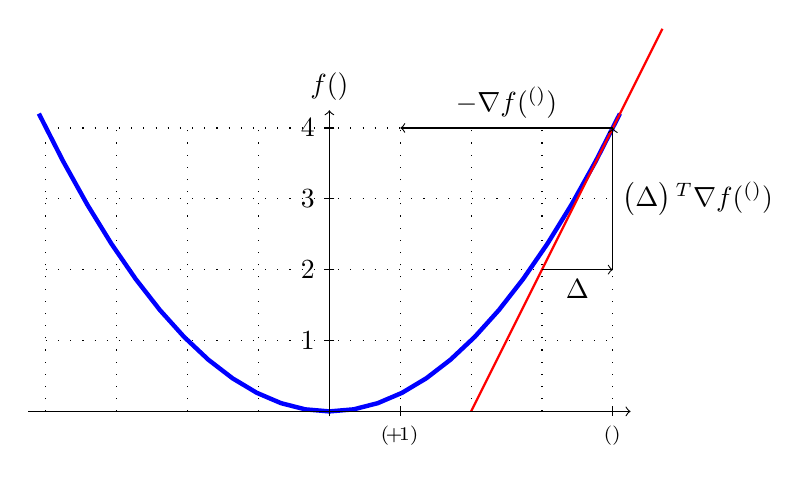
\begin{tikzpicture}[scale=0.9]
					\draw[loosely dotted] (-4,0) grid (4,4);
					\draw[blue, ultra thick, domain=-4.1:4.1] plot (\x,  {(1/4)*\x*\x});
					\draw[red, thick, domain=2:4.7] plot (\x,  {2*\x - 4});
					\draw[<-] (4,4) -- node[right] {$\big( \Delta \weights\big)\,^{T} \nabla f(\weights^{(\itercntr)})$} (4,2);
					\draw[->] (4,4) -- node[above] {$-\lrate \nabla f(\weights^{(\itercntr)})$} (1,4);
					\draw[<-] (4,2) -- node[below] {$\Delta \weights$} (3,2) ;
					\draw[->] (-4.25,0) -- (4.25,0) node[right] {$\weights$};
					\draw[->] (0,-2pt) -- (0,4.25) node[above] {$f(\weights)$};
					\draw[shift={(0,0)}] (0pt,2pt) -- (0pt,-2pt) node[below] {$\overline{\weights}$};
					\draw[shift={(4,0)}] (0pt,2pt) -- (0pt,-2pt) node[below] {$\weights^{(\itercntr)}$};
					\draw[shift={(1,0)}] (0pt,2pt) -- (0pt,-2pt) node[below] {$\weights^{(\itercntr\!+\!1)}$};
					\foreach \y/\ytext in {1/1, 2/2, 3/3, 4/4}
					\draw[shift={(0,\y)}] (2pt,0pt) -- (-2pt,0pt) node[left] {$\ytext$};  
				\end{tikzpicture}
			\end{center}
			\caption{A single \gls{gradstep} \eqref{equ_def_GD_step_dict} towards the minimizer $\overline{\weights}$ of $f(\weights)$.}
			\label{fig_basic_GD_step_dict}
		\end{figure}
		\foreignlanguage{greek}{Βλέπε επίσης:} \gls{minimum}, \gls{differentiable}, \gls{function}, \gls{gradstep}, \gls{stepsize}, \gls{gradient}.},
	first={\foreignlanguage{greek}{κάθοδος κλίσης}},
	text={\foreignlanguage{greek}{κάθοδος κλίσης}},
	user1={\foreignlanguage{greek}{κάθοδος κλίσης}}, %nominative
	user2={\foreignlanguage{greek}{καθόδου κλίσης}}, %genitive  
	user3={\foreignlanguage{greek}{καθόδο κλίσης}} %accusative 
}

\newglossaryentry{sgd}
{name={\foreignlanguage{greek}{κάθοδος υποκλίσης}}, 
	description={\Gls{subgradient}\index{\foreignlanguage{greek}{κάθοδος υποκλίσης}} 
		descent is a \gls{generalization} of \gls{gd} that does not require differentiability of the 
		\gls{function} to be minimized. This \gls{generalization} is obtained by replacing the concept 
		of a \gls{gradient} with that of a \gls{subgradient}. Similar to \gls{gradient}s, \gls{subgradient}s 
		allow us to construct local approximations of an \gls{objfunc}. The \gls{objfunc} 
		might be the \gls{emprisk} $\emperror\big( \hypothesis^{(\weights)} \big| \dataset \big)$ viewed 
		as a \gls{function} of the \gls{modelparams} $\weights$ that select a \gls{hypothesis} $\hypothesis^{(\weights)} \in \hypospace$.\\
		\foreignlanguage{greek}{Βλέπε επίσης:} \gls{subgradient}, \gls{generalization}, \gls{gd}, \gls{function}, \gls{gradient}, 
		\gls{objfunc}, \gls{emprisk}, \gls{modelparams}, \gls{hypothesis}.},
	first={\foreignlanguage{greek}{κάθοδος υποκλίσης}},
	text={\foreignlanguage{greek}{κάθοδος υποκλίσης}},
	user1={\foreignlanguage{greek}{κάθοδος υποκλίσης}}, %nominative
	user2={\foreignlanguage{greek}{καθόδου υποκλίσης}} %genitive  
}

\newglossaryentry{datanorm}
{name={\foreignlanguage{greek}{κανονικοποίηση δεδομένων}},
	description={\foreignlanguage{greek}{Η κανονικοποίηση} \glsentryuserii{data}\index{\foreignlanguage{greek}{κανονικοποίηση δεδομένων}} 
		\foreignlanguage{greek}{αναφέρεται σε μετασχηματισμούς που εφαρμόζονται στα} \glsentryuservi{featurevec} \glsentryuserv{datapoint} 
		\foreignlanguage{greek}{για να βελτιωθούν οι} \glsentryuseri{statasp} \foreignlanguage{greek}{ή οι} \glsentryuseri{compasp} 
		\foreignlanguage{greek}{της μεθόδου} \glsentryuserii{ml}. \foreignlanguage{greek}{Για παράδειγμα, στη} \glsentryuseriii{linreg} 
		\foreignlanguage{greek}{με} \glsentryuseriii{gdmethods} \foreignlanguage{greek}{που χρησιμοποιούν έναν σταθερό}
		\glsentryuseriii{learnrate}, \foreignlanguage{greek}{η σύγκλιση εξαρτάται από τον έλεγχο της} \glsentryuserii{norm} \glsentryuserv{featurevec} 
		\foreignlanguage{greek}{στο} \glsentryuseriii{trainset}. \foreignlanguage{greek}{Μία κοινή προσέγγιση είναι να κανονικοποιούμε τα} 
		\glsentryuservi{featurevec}, \foreignlanguage{greek}{έτσι ώστε η} 
		\gls{norm} \foreignlanguage{greek}{τους να μην υπερβαίνει το ένα} \cite[\foreignlanguage{greek}{Κεφ.}\ 5]{MLBasics}.\\
		\foreignlanguage{greek}{Βλέπε επίσης:} \gls{data}, \gls{featurevec}, \gls{datapoint}, \gls{ml}, \gls{statasp}, \gls{compasp}, 
		\gls{linreg}, \gls{gdmethods}, \gls{learnrate}, \gls{norm}, \gls{trainset}.},
	first={\foreignlanguage{greek}{κανονικοποίηση δεδομένων}},
	text={\foreignlanguage{greek}{κανονικοποίηση δεδομένων}},
	user1={\foreignlanguage{greek}{κανονικοποίηση δεδομένων}}, %nominative
  	user2={\foreignlanguage{greek}{κανονικοποίησης δεδομένων}} %genitive 
}

\newglossaryentry{probdist}
{name={\foreignlanguage{greek}{κατανομή πιθανότητας}},
	description={\foreignlanguage{greek}{Για να αναλύσουμε μεθόδους}\index{\foreignlanguage{greek}{κατανομή πιθανότητας}} 
		\glsentryuserii{ml}, \foreignlanguage{greek}{μπορεί να είναι χρήσιμο να ερμηνεύσουμε} \glsentryuservi{datapoint} \foreignlanguage{greek}{ως} 
		\glsentryuseriii{iid} \glsentryuservi{realization} \foreignlanguage{greek}{μίας} \glsentryuserii{rv}. \foreignlanguage{greek}{Οι τυπικές  
		ιδιότητες τέτοιων} \glsentryuserv{datapoint} \foreignlanguage{greek}{διέπονται τότε από την κατανομή} \glsentryuserii{probability}  
		\foreignlanguage{greek}{αυτής της} \glsentryuserii{rv}. \foreignlanguage{greek}{Η κατανομή} \glsentryuserii{probability} 
		\foreignlanguage{greek}{μίας δυαδικής} \glsentryuserii{rv} $\truelabel \in \{0,1\}$ \foreignlanguage{greek}{προσδιορίζεται πλήρως
		από τις πιθανότητες $\prob{\truelabel = 0}$ και 
		$\prob{\truelabel=1}\!=\!1\!-\!\prob{\truelabel=0}$. Η κατανομή} \glsentryuserii{probability} 
		\foreignlanguage{greek}{μίας} \glsentryuserii{rv} \foreignlanguage{greek}{πραγματικής τιμής $\feature \in \mathbb{R}$ μπορεί να 
		προσδιορίζεται από μία} \glsentryuseriii{pdf} $p(\feature)$, \foreignlanguage{greek}{έτσι ώστε $\prob{ \feature \in [a,b] } \approx  p(a) |b-a|$. 
	    	Στην πιο γενική περίπτωση, η κατανομή} \glsentryuserii{probability} \foreignlanguage{greek}{ορίζεται από ένα μέτρο} 
		\glsentryuserii{probability} \cite{BillingsleyProbMeasure}, \cite{GrayProbBook}.\\
	    	\foreignlanguage{greek}{Βλέπε επίσης:} \gls{ml}, \gls{datapoint}, \gls{iid}, \gls{realization}, \gls{rv}, \gls{probability}, \gls{pdf}. },
	 first={\foreignlanguage{greek}{κατανομή πιθανότητας}},
	 text={\foreignlanguage{greek}{κατανομή πιθανότητας}},
	 user1={\foreignlanguage{greek}{κατανομή πιθανότητας}}, %nominative
	 user2={\foreignlanguage{greek}{κατανομής πιθανότητας}}, %genitive  
	 user3={\foreignlanguage{greek}{κατανομή πιθανότητας}}, %accusative 
	 user4={\foreignlanguage{greek}{κατανομές πιθανοτήτων}}, %nominativepl
	 user5={\foreignlanguage{greek}{κατανομών πιθανοτήτων}}, %genitivepl  
	 user6={\foreignlanguage{greek}{κατανομές πιθανοτήτων}}, %accusativepl 
	 user7={\foreignlanguage{greek}{κατανομής πιθανότητάς}} %genitivedoublestress
}

\newglossaryentry{backdoor}
{name={\foreignlanguage{greek}{κερκόπορτα}}, 
	description={\foreignlanguage{greek}{Μία επίθεση κερκόπορτας}\index{\foreignlanguage{greek}{κερκόπορτα}} 
		(backdoor) \foreignlanguage{greek}{αναφέρεται στον σκόπιμο χειρισμό της διαδικασίας εκπαίδευσης που αποτελεί τη βάσης 
		μίας μεθόδου} \glsentryuserii{ml}. \foreignlanguage{greek}{Αυτός ο χειρισμός μπορεί να υλοποιηθεί με τη διαταραχή του} \glsentryuserii{trainset} 
		\foreignlanguage{greek}{(δηλαδή μέσω τ..} \gls{datapoisoning}) \foreignlanguage{greek}{ή μέσω του}  
		\glsentryuserii{algorithm} \foreignlanguage{greek}{βελτιστοποίησης που χρησιμοποιείται από μία μέθοδο βασισμένη 
		στην} \glsentryuseriii{erm}. \foreignlanguage{greek}{Ο στόχος μίας επίθεσης κερκόπορτας είναι να  
		ωθήσει την} \glsentryuseriii{hypothesis} $\learnthypothesis$ \foreignlanguage{greek}{που έχει μαθευτεί
		προς συκεκριμένες} \glsentryuservi{prediction} \foreignlanguage{greek}{για ένα ορισμένο πεδίο τιμών} \glsentryuserv{feature}. 
		\foreignlanguage{greek}{Το συγκεκριμένο πεδίο τιμών} \glsentryuserv{feature} 
		\foreignlanguage{greek}{χρησιμεύει ως το κλειδί (ή έναυσμα) για να ξεκλειδώσει μία κερκόπορτα με την έννοια  
		της παροχής ανώμαλων} \glsentryuserv{prediction}. \foreignlanguage{greek}{Το κλειδί $\featurevec$ και η σχετική 
		ανώμαλη} \glsentryuseri{prediction} $\learnthypothesis(\featurevec)$ \foreignlanguage{greek}{είναι γνωστά μόνο στον επιτιθέμενο.}\\
		\foreignlanguage{greek}{Βλέπε επίσης:} \gls{ml}, \gls{trainset}, \gls{datapoisoning}, \gls{algorithm}, \gls{erm}, \gls{hypothesis}, \gls{prediction}, \gls{feature}.},
	first={\foreignlanguage{greek}{κερκόπορτα}},
	text={\foreignlanguage{greek}{κερκόπορτα}},
	user1={\foreignlanguage{greek}{κερκόπορτα}}, %nominative
	user2={\foreignlanguage{greek}{κερκόπορτας}} %genitive  
}

\newglossaryentry{gradient}
{name={\foreignlanguage{greek}{κλίση}},
	description={\foreignlanguage{greek}{Για μία}\index{\foreignlanguage{greek}{κλίση}} 
		\glsentryuseriii{function} \foreignlanguage{greek}{πραγματικής τιμής 
		$f: \mathbb{R}^{\featuredim} \rightarrow \mathbb{R}: \weights \mapsto f(\weights)$, 
		αν υφίσταται ένα διάνυσμα $\vg$ τέτοιο ώστε 
		$$\lim_{\weights \rightarrow \weights'} {f(\weights) - \big(f(\weights') + \vg\,^{T} (\weights - \weights') \big) }/{\| \weights - \weights'\|}=0$$
		αναφέρεται ως η κλίση της $f$ στο $\weights'$. Αν υφίσταται, η κλίση είναι μοναδική και δηλώνεται  
		ως $\nabla f(\weights')$ ή} $\nabla f(\weights)\big|_{\weights'}$ \cite{RudinBookPrinciplesMatheAnalysis}.\\
		\foreignlanguage{greek}{Βλέπε επίσης:} \gls{function}. },
	first={\foreignlanguage{greek}{κλίση}},
	text={gradient},
	user1={\foreignlanguage{greek}{κλίση}}, %nominative
  	user2={\foreignlanguage{greek}{κλίσης}}, %genitive   
	user3={\foreignlanguage{greek}{κλίση}}, %accusative   
	user4={\foreignlanguage{greek}{κλίσεις}}, %nominativepl
  	user5={\foreignlanguage{greek}{κλίσεων}}, %genitivepl   
	user6={\foreignlanguage{greek}{κλίσεις}} %accusativepl 
}

\newglossaryentry{stopcrit}
{name={\foreignlanguage{greek}{κριτήριο τερματισμού}},
	description={\foreignlanguage{greek}{Πολλές μέθοδοι}\index{\foreignlanguage{greek}{κριτήριο τερματισμού}} 
		\glsentryuserii{ml} \foreignlanguage{greek}{χρησιμοποι\-ούν επαναληπτικούς} \glsentryuservi{algorithm} 
		\foreignlanguage{greek}{που κατασκευάζουν μία ακολουθία} \glsentryuserii{modelparams} 
		\foreignlanguage{greek}{προκειμένου να ελαχιστοποιήσουν το} \glsentryuseriii{trainerr}. 
		\foreignlanguage{greek}{Για παράδειγμα, οι} \glsentryuseri{gdmethods} \foreignlanguage{greek}{ενημερώνουν 
		επαναληπτικά τις} \glsentryuservi{parameter} \foreignlanguage{greek}{ενός παραμετρικού} \glsentryuserii{model}, 
		\foreignlanguage{greek}{όπως ενός} \glsentryuserii{linmodel} \foreignlanguage{greek}{ή ενός} \glsentryuserii{deepnet}. 
		\foreignlanguage{greek}{Δεδομένων περιορισμένων υπολογιστικών πόρων, χρειάζεται να σταματήσουμε
		την ενημέρωση των} \glsentryuserv{parameter} \foreignlanguage{greek}{μετά από έναν
		πεπερασμένο αριθμό επαναλήψεων. Ένα κριτήριο τερματισμού είναι οποιαδήποτε καλά ορισμένη συνθήκη
		για να αποφασίσουμε πότε να σταματήσουμε την ενημέρωση.}  \\
		\foreignlanguage{greek}{Βλέπε επίσης:} \gls{ml}, \gls{algorithm}, \gls{modelparams}, \gls{trainerr}, \gls{gdmethods}, 
		\gls{parameter}, \gls{model}, \gls{linmodel}, \gls{deepnet}.},
	first={\foreignlanguage{greek}{κριτήριο τερματισμού}},
	text={\foreignlanguage{greek}{κριτήριο τερματισμού}},
	user1={\foreignlanguage{greek}{κριτήριο τερματισμού}}, %nominative
	user2={\foreignlanguage{greek}{κριτηρίου τερματισμού}} %genitive
}

 \newglossaryentry{cvxclustering}
 {name={\foreignlanguage{greek}{κυρτή συσταδοποίηση}}, 
 	description={\foreignlanguage{greek}{Θεωρούμε ένα}\index{\foreignlanguage{greek}{κυρτή συσταδοποίηση}} 
		\glsentryuseriii{dataset} $\featurevec^{(1)}, \ldots, \featurevec^{(\samplesize)} \in \mathbb{R}^{\nrfeatures}$. 
 		\foreignlanguage{greek}{Η} \glsentryuseriii{convex} \glsentryuseri{clustering} \foreignlanguage{greek}{μαθαίνει διανύσματα 
		$\weights^{(1)}, \ldots, \weights^{(\samplesize)}$ ελαχιστοποιώντας το} 
 		$$\sum_{\sampleidx=1}^{\samplesize} \normgeneric{\featurevec^{(\sampleidx)} - \weights^{(\sampleidx)}}{2}^2 + 
 		\regparam \sum_{\nodeidx,\nodeidx' \in \nodes} \normgeneric{\weights^{(\nodeidx)} - \weights^{(\nodeidx')}}{p}.$$ 
		\foreignlanguage{greek}{Εδώ,} $\normgeneric{\vu}{p} \defeq \big( \sum_{\featureidx=1}^{\dimlocalmodel} |u_{\featureidx}|^{p} \big)^{1/p}$ 
		\foreignlanguage{greek}{δηλώνει την} $p$-\glsentryuseriii{norm} (\foreignlanguage{greek}{για} $p\geq1$).  
		\foreignlanguage{greek}{Προκύπτει ότι πολλά από τα βέλτιστα διανύσματα} $\widehat{\weights}^{(1)}, \ldots, \widehat{\weights}^{(\samplesize)}$ 
		\foreignlanguage{greek}{συμπίπτουν. Μία} \glsentryuseri{cluster} \foreignlanguage{greek}{τότε αποτελείται από αυτά τα} 
		\glsentryuservi{datapoint}\linebreak $\sampleidx \in \{1, \ldots, \samplesize\}$ 
		\foreignlanguage{greek}{με ταυτόσημα} $\widehat{\weights}^{(\sampleidx)}$ \cite{JMLR:v22:18-694}, \cite{Pelckmans2005}.\\
		\foreignlanguage{greek}{Βλέπε επίσης:} \gls{dataset}, \gls{convex}, \gls{clustering}, \gls{norm}, \gls{cluster}, \gls{datapoint}. },
 	first={\foreignlanguage{greek}{κυρτή συσταδοποίηση}},
	text={\foreignlanguage{greek}{κυρτή συσταδοποίηση}},
	user1={\foreignlanguage{greek}{κυρτή συσταδοποίηση}}, %nominative
	user2={\foreignlanguage{greek}{κυρτής συσταδοποίησης}} %genitive  
}

\newglossaryentry{convex}
{name={\foreignlanguage{greek}{κυρτός}},
	description={\foreignlanguage{greek}{Ένα υποσύνολο}\index{\foreignlanguage{greek}{κυρτός}} 
		$\mathcal{C} \subseteq \mathbb{R}^{\featuredim}$  
		\foreignlanguage{greek}{του} \glsentryuserii{euclidspace} $\mathbb{R}^{\featuredim}$ \foreignlanguage{greek}{αναφέρεται ως κυρτό αν περιέχει  
		το ευθύγραμμο τμήμα μεταξύ οποιωνδήποτε δύο σημεί\-ων $\vx, \vy\!\in\!\cluster$ σε ένα σύνολο. Μία} \glsentryuseri{function}  
		$f\!:\!\mathbb{R}^{\dimlocalmodel}\!\rightarrow\!\mathbb{R}$ \foreignlanguage{greek}{είναι κυρτή αν το} 
		\glsentryuserii{epigraph} \foreignlanguage{greek}{της} $\big\{ \big( \weights\,^{T},t \big)\,^{T}\!\in\!\mathbb{R}^{\dimlocalmodel\!+\!1}\!:\!t\!\geq\!f(\weights) \}$ 
		\foreignlanguage{greek}{είναι ένα κυρτό σύνολο} \cite{BoydConvexBook}. \foreignlanguage{greek}{Παρουσιάζουμε ένα παράδειγμα 
		ενός κυρτού συνόλου και μίας κυρτής} \glsentryuserii{function} \foreignlanguage{greek}{στο Σχ.} \ref{fig_convex_set_function_dict}. 
		\begin{figure}[H]
		\begin{center}
			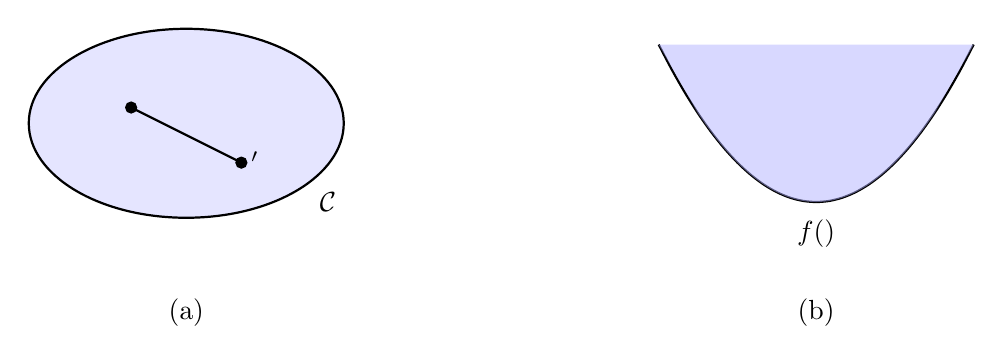
\begin{tikzpicture}
				\fill[blue!20, opacity=0.5] (-3,0) ellipse (2 and 1.2); 
				\draw[thick] (-3,0) ellipse (2 and 1.2);
				\filldraw[black] (-3.7,0.2) circle (2pt) node[left] {$\vw$};
				\filldraw[black] (-2.3,-0.5) circle (2pt) node[right] {$\vw'$};
				\draw[thick] (-3.7,0.2) -- (-2.3,-0.5);
				\node at (-1.2,-1.0) {$\mathcal{C}$};
				\node at (-3,-2.4) {(a)};
				\begin{scope}[shift={(5,-1)}]
					\draw[thick, domain=-2:2, smooth, variable=\x] 
					plot ({\x}, {0.5*\x*\x});
					\fill[blue!30, opacity=0.5] 
					plot[domain=-1.5:1.5, smooth] ({\x}, {0.5*\x*\x}) -- 
					(2, {0.5*2*2}) -- 
					(-2, {0.5*2*2}) -- 
					cycle;
					\node at (0,-0.4) {$f(\weights)$};
					\node at (0,-1.4) {(b)};
				\end{scope}
			\end{tikzpicture}
			\vspace*{-8mm}
			\end{center}
			{\selectlanguage{greek}
			\caption{\selectlanguage{english}{(a)} \foreignlanguage{greek}{Ένα κυρτό σύνολο} $\cluster \subseteq \mathbb{R}^{\dimlocalmodel}$. 
				\selectlanguage{english}{(b)} \foreignlanguage{greek}{Μία κυρτή} \glsentryuseri{function} $f: \mathbb{R}^{\dimlocalmodel} \rightarrow \mathbb{R}$.
				\label{fig_convex_set_function_dict}} }
		\end{figure}
		\foreignlanguage{greek}{Βλέπε επίσης:} \gls{euclidspace}, \gls{function}, \gls{epigraph}.},
	first={\foreignlanguage{greek}{κυρτός}},
	text={convex},
	user1={\foreignlanguage{greek}{κυρτός}}, %nominative
	user2={\foreignlanguage{greek}{κυρτού}}, %genitive 
	user3={\foreignlanguage{greek}{κυρτή}} %nominativeoraccusativefem
}

\newglossaryentry{smooth}
{name={\foreignlanguage{greek}{λεία}},
	description={A\index{\foreignlanguage{greek}{λεία}} 
		real-valued \gls{function} $f: \mathbb{R}^{\dimlocalmodel} \rightarrow \mathbb{R}$ 
		is smooth if it is \gls{differentiable} and its \gls{gradient} $\nabla f(\weights)$ is continuous at all 
		$\weights \in \mathbb{R}^{\dimlocalmodel}$  \cite{nesterov04}, \cite{CvxBubeck2015}. A smooth \gls{function} $f$ is referred to 
		as $\beta$-smooth if the \gls{gradient} $\nabla f(\weights)$ is Lipschitz continuous with Lipschitz constant $\beta$, i.e., 
		$$\| \nabla f(\weights) - \nabla f(\weights') \| \leq \beta \| \weights - \weights' \| \mbox{, for any } \weights,\weights' \in \mathbb{R}^{\dimlocalmodel}.$$ 
		The constant $\beta$ quantifies the smoothness of the \gls{function} $f$: the smaller the $\beta$, 
		the smoother $f$ is. \Gls{optproblem}s with a smooth \gls{objfunc} can be solved effectively by \gls{gdmethods}. 
	   	Indeed, \gls{gdmethods} approximate the \gls{objfunc} locally around a current choice $\weights$ 
	    	using its \gls{gradient}. This approximation works well if the \gls{gradient} does 
	    	not change too rapidly. We can make this informal claim precise by studying the effect of a single 
	    	\gls{gradstep} with \gls{stepsize} $\lrate=1/\beta$ (see Fig. \ref{fig_gd_smooth_dict}). 
	    	\begin{figure}[H] 
	    	\begin{center} 
	    	\begin{tikzpicture}[scale=0.8, x=0.6cm,y=0.05cm]
	    		% Parameter to shift the quadratic curve horizontally
	    		\def\hshift{0.5} % Change this value to shift the curve horizontally
	    		% Define the function (only the increasing part of x^2 for x >= 0)
	    		\draw[thick, dashed, domain=\hshift:8+\hshift, smooth, variable=\x] plot ({\x}, {\x^2}); %node[right] {$f(x) = x^2$};
	    		% Define points for the tangents
	    		\coordinate (w) at (\hshift,{\hshift*\hshift}); % Point w on the curve (left end of the plot)
	    		\coordinate (wkplus1) at (4+\hshift,{(4+\hshift)^2}); % Point w^{k+1} on the curve (x=1 + hshift, y=1)
	    		\coordinate (wk) at (8+\hshift,{(8+\hshift)^2}); % Point w^k on the curve (right end of the plot)
	    		% Calculate the slopes for the tangents
  				\draw[line width=1pt, transform canvas={yshift=-1pt}] (wk) -- +(-2, -{4*(8 + \hshift)} ) -- +(1, {2*(8 + \hshift)}); % Tangent at w^k with positive slope
 				\draw[line width=1pt, transform canvas={yshift=-1pt}] (w) -- +(-1, {-{2*\hshift}} ) -- +(1, {+{2*\hshift}})  node[below] {$\nabla f(\weights)$};% Tangent at w with slope 0 (since derivative at hshift = 0)
%	    		% Draw filled circles at points w^k, w, and w^{k+1}
	    		\filldraw (wk) circle (2pt) node[above left] {$\weights^{(\iteridx)}$} node[below right, xshift=-15pt,yshift=-15pt] {$\nabla f(\weights^{(\iteridx)})$} ;
	    		\filldraw (w) circle (2pt) node[above right] {$\weights$} ;
	    		\filldraw (wkplus1) circle (2pt) node[below right] {$\weights^{(\iteridx+1)}\!=\!\weights^{(\iteridx)}\!-\!(1/\beta)\nabla f(\weights^{(\iteridx)})$};
	    		    % Draw horizontal rulers to mark the function values at wk and wk_plus1
	    		\draw[dashed] (wk) -- ($(8,0) + (wk)$) ; %node[left] {$f(\weights^{(\iteridx)})$};
	    		\draw[dashed] (wkplus1) -- ($(12,0) + (wkplus1)$) ; %node[left] {$f(\weights^{(\iteridx+1)})$};
	    		 \draw[<->, thick] ($(4,0) + (wk)$) -- ($(8,0) + (wkplus1)$) 
	    		node[midway, right] {$ f\big(\weights^{(\iteridx)}\big)\!-\!f\big(\weights^{(\iteridx+1)}\big)\!\geq\!\frac{1}{2\beta}\normgeneric{\nabla f(\weights^{(\iteridx)})}{2}^{2}$};
%	    		% Label the curve
%	    		\node at (2, 4) {};
	    	\end{tikzpicture}
	    	\end{center}
	    	\caption{Consider an \gls{objfunc} $f(\weights)$ that is $\beta$-smooth. Taking a \gls{gradstep}, with \gls{stepsize} $\lrate = 1/\beta$, decreases the 
	    		objective by at least ${1}/{2\beta}\normgeneric{\nabla f(\weights^{(\iteridx)})}{2}^{2}$ \cite{nesterov04}, \cite{CvxBubeck2015}, \cite{CvxAlgBertsekas}. 
	    		Note that the \gls{stepsize} $\lrate = 1/\beta$ becomes larger for smaller $\beta$. Thus, for smoother \gls{objfunc}s (i.e., those with smaller $\beta$), 
			we can take larger steps. \label{fig_gd_smooth_dict}}
	    	\end{figure}
		\foreignlanguage{greek}{Βλέπε επίσης:} \gls{function}, \gls{differentiable}, \gls{gradient}, \gls{optproblem}, \gls{objfunc}, \gls{gdmethods}, 
		\gls{gradstep}, \gls{stepsize}. },
	first={\foreignlanguage{greek}{λεία}},
	text={\foreignlanguage{greek}{λεία}},
	user1={\foreignlanguage{greek}{λεία}}, %nominative
	user2={\foreignlanguage{greek}{λείας}}, %genitive
	user3={\foreignlanguage{greek}{λεία}} %accusative
}

\newglossaryentry{logloss}
{name={\foreignlanguage{greek}{λογιστική απώλεια}}, 
	description={Consider\index{\foreignlanguage{greek}{λογιστική απώλεια}} 
		a \gls{datapoint} characterized by the \gls{feature}s $\featurevec$ and a binary \gls{label} $\truelabel \in \{-1,1\}$. 
		We use a real-valued \gls{hypothesis} $\hypothesis$ to predict the \gls{label} $\truelabel$ 
		from the \gls{feature}s $\featurevec$. The logistic \gls{loss} incurred by this \gls{prediction} is 
		defined as 
		\begin{equation} 
		\label{equ_log_loss_gls_dict}
		\lossfunc{(\featurevec,\truelabel)}{\hypothesis} \defeq  \log\, ( 1 + \exp\,(- \truelabel \hypothesis(\featurevec))).
		\end{equation}
		\begin{figure}[H]
		\begin{center}
			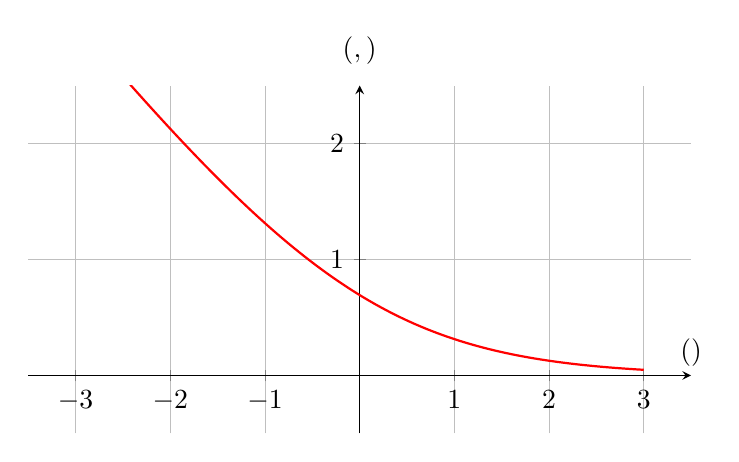
\begin{tikzpicture}
				\begin{axis}[
				axis lines=middle,
				xlabel={$\truelabel\hypothesis(\featurevec)$},
				ylabel={$\lossfunc{(\featurevec,\truelabel)}{\hypothesis}$},
				xlabel style={at={(axis description cs:1.,0.3)}, anchor=north},  % Adjusted to be relative to axis end
				ylabel style={at={(axis description cs:0.5,1.1)}, anchor=center}, % Corrected to vertical position, rotated for readability
				xmin=-3.5, xmax=3.5,
				ymin=-0.5, ymax=2.5,
				xtick={-3, -2, -1, 0, 1, 2, 3},
				ytick={0, 1, 2},
				domain=-3:3,
				samples=100,
				width=10cm, height=6cm,
				grid=both,
				major grid style={line width=.2pt, draw=gray!50},
				minor grid style={line width=.1pt, draw=gray!20},
				legend pos=south west % Positions legend at the bottom left
				]
					\addplot [red, thick] {ln(1 + exp(-x))};    
				\end{axis}
			\end{tikzpicture}
		\caption{The logistic \gls{loss} incurred by the \gls{prediction} $\hypothesis(\featurevec) \in \mathbb{R}$ 
			for a \gls{datapoint} with \gls{label} $\truelabel \in \{-1,1\}$.}
		\label{fig_logloss_dict}
		\end{center}
		\end{figure}
		Note that the expression \eqref{equ_log_loss_gls_dict} for the logistic \gls{loss} applies only for the \gls{labelspace} 
		$\labelspace = \{ -1,1\}$ and when using the thresholding rule \eqref{equ_def_threshold_bin_classifier_dict}.\\
		\foreignlanguage{greek}{Βλέπε επίσης:} \gls{datapoint}, \gls{feature}, \gls{label}, \gls{hypothesis}, \gls{loss}, \gls{prediction}, \gls{labelspace}.},
	first={\foreignlanguage{greek}{λογιστική απώλεια}},
	text={\foreignlanguage{greek}{λογιστική απώλεια}},
	user1={\foreignlanguage{greek}{λογιστική απώλεια}}, %nominative
	user2={\foreignlanguage{greek}{λογιστικής απώλειας}}, %genitive   
	user3={\foreignlanguage{greek}{λογιστική απώλεια}} %accusative
}

\newglossaryentry{logreg}
{name={\foreignlanguage{greek}{λογιστική παλινδρόμηση}}, 
	description={\foreignlanguage{greek}{Η λογιστική}\index{\foreignlanguage{greek}{λογιστική παλινδρόμηση}} 
		\glsentryuseri{regression} \foreignlanguage{greek}{μαθαίνει μία γραμμική} \gls{map} \glsentryuserii{hypothesis} (\foreignlanguage{greek}{ή έναν}  
		\glsentryuseriii{classifier}) $\hypothesis(\featurevec) = \weights\,^{T} \featurevec$ 
		\foreignlanguage{greek}{για να προβλέψει μία δυαδική} \glsentryuseriii{label} $\truelabel$ \foreignlanguage{greek}{με βάση 
		το αριθμητικό} \glsentryuseriii{featurevec} $\featurevec$ \foreignlanguage{greek}{ενός} 
		\glsentryuserii{datapoint}. \foreignlanguage{greek}{Η ποιότητα μίας γραμμικής} \gls{map} \glsentryuserii{hypothesis} 
		\foreignlanguage{greek}{μετράται από τη μέση} \glsentryuseriii{logloss} \foreignlanguage{greek}{σε κάποια}
		\glsentryuservi{labeled datapoint} (\foreignlanguage{greek}{δηλαδή το} \glsentryuseriii{trainset}).\\
		\foreignlanguage{greek}{Βλέπε επίσης:} \gls{regression}, \gls{hypothesis}, \gls{map}, \gls{classifier}, \gls{label}, \gls{featurevec}, 
		\gls{datapoint}, \gls{logloss}, \gls{labeled datapoint}, \gls{trainset}.},
	first={\foreignlanguage{greek}{λογιστική παλινδρόμηση}},
	text={\foreignlanguage{greek}{λογιστική παλινδρόμηση}},
	user1={\foreignlanguage{greek}{λογιστική παλινδρόμηση}}, %nominative
	user2={\foreignlanguage{greek}{λογιστικής παλινδρόμησης}} %genitive   
}

\newglossaryentry{multitask learning}
{name={\foreignlanguage{greek}{μάθηση πολυδιεργασίας}},
	description={\foreignlanguage{greek}{Η μάθηση πολυδιεργασίας στοχεύει να αξιοποιήσει}\index{\foreignlanguage{greek}{μάθηση πολυδιεργασίας}} 
		\foreignlanguage{greek}{σχέσεις μεταξύ διαφορετικών} \glsentryuserv{learningtask}. \foreignlanguage{greek}{Θεωρούμε δύο} 
		\glsentryuservi{learningtask} \foreignlanguage{greek}{που προκύπτουν από το ίδιο}  
	 	\glsentryuseriii{dataset} \foreignlanguage{greek}{λήψεων από κάμερα υπολογιστή. Η πρώτη εργασία είναι να προβλεφθεί η 
		παρουσία ενός ανθρώπου, ενώ η δεύτερη εργασία είναι να προβλεφθεί η παρουσία ενός αυτοκινήτου. 
	 	Μπορεί να είναι χρήσιμο να χρησιμοποιηθεί η ίδια δομή} \glsentryuserii{deepnet} \foreignlanguage{greek}{και για τις δύο 
		εργασίες και να επιτραπεί μόνο τα} \glsentryuseri{weights} \foreignlanguage{greek}{του τελικού επιπέδου εξόδου να είναι διαφορετικά.} \\
	 	\foreignlanguage{greek}{Βλέπε επίσης:} \gls{learningtask}, \gls{dataset}, \gls{deepnet}, \gls{weights}.},
	first={\foreignlanguage{greek}{μάθηση πολυδιεργασίας}},
	text={\foreignlanguage{greek}{μάθηση πολυδιεργασίας}},
	user1={\foreignlanguage{greek}{μάθηση πολυδιεργασίας}}, %nominative
	user2={\foreignlanguage{greek}{μάθησης πολυδιεργασίας}} %genitive 
}

\newglossaryentry{featlearn}
{name={\foreignlanguage{greek}{μάθηση χαρακτηριστικών}},
	description={\foreignlanguage{greek}{Θεωρούμε μία εφαρμογή} \glsentryuserii{ml} \foreignlanguage{greek}{με} \glsentryuservi{datapoint} 
		\foreignlanguage{greek}{που χαρακτηρίζονται από ακατέργαστα} \glsentryuservi{feature} $\featurevec \in \featurespace$. 
		\foreignlanguage{greek}{Η μάθηση} \glsentryuserv{feature}\index{\foreignlanguage{greek}{μάθηση χαρακτηριστικών}} 
		\foreignlanguage{greek}{αναφέρεται στην εργασία της μάθησης μίας} \gls{map} 
		$$\featuremapvec: \featurespace \rightarrow \featurespace': \featurevec \mapsto \featurevec'$$ 
		\foreignlanguage{greek}{που διαβάζει τα} \glsentryuservi{feature} $\featurevec \in \featurespace$ 
		\foreignlanguage{greek}{ενός} \glsentryuserii{datapoint} \foreignlanguage{greek}{και παραδίδει νέα}  
		\glsentryuservi{feature} $\featurevec' \in \featurespace'$ \foreignlanguage{greek}{από έναν νέο} \glsentryuseriii{featurespace} $\featurespace'$. 
		\foreignlanguage{greek}{Διαφορετικές μέθοδοι μάθησης} \glsentryuserv{feature} \foreignlanguage{greek}{προκύπτουν για διαφορετικές επιλογές 
		σχεδιασμού των $\featurespace,\featurespace'$, για έναν} \glsentryuseriii{hypospace} $\hypospace$ 
		\foreignlanguage{greek}{πιθανών} \gls{map}s $\featuremapvec$, \foreignlanguage{greek}{και για ένα ποσοτικό μέτρο της 
		χρησιμότητας μίας συγκεκριμένης $\featuremapvec \in \hypospace$. Για παράδειγμα, η} \glsentryuseri{pca} 
		\foreignlanguage{greek}{χρησιμοποιεί $\featurespace \defeq \mathbb{R}^{\dimlocalmodel}$, $\featurespace' \defeq \mathbb{R}^{\dimlocalmodel'}$ 
		με $\dimlocalmodel' < \dimlocalmodel$, και έναν} \glsentryuseriii{hypospace} 
		$$\hypospace\defeq \big\{ \featuremapvec: \mathbb{R}^{\dimlocalmodel}
		\!\rightarrow\! \mathbb{R}^{\dimlocalmodel'}\!:\!\featurevec'\!\defeq\!\mF \featurevec \mbox{ \foreignlanguage{greek}{με κάποια} } \mF \!\in\! \mathbb{R}^{\dimlocalmodel' \!\times \dimlocalmodel} \big\}.$$ 
		\foreignlanguage{greek}{Η} \glsentryuseri{pca} \foreignlanguage{greek}{μετράει τη χρησιμότητα μίας συγκεκριμένης} \gls{map} 
		$\featuremapvec(\featurevec)= \mF \featurevec$ \foreignlanguage{greek}{από το} \glsentryuseriii{minimum} \foreignlanguage{greek}{γραμμικό σφάλμα 
		ανακατασκευής που προκαλείται σε ένα} \glsentryuseriii{dataset}, \foreignlanguage{greek}{έτσι ώστε}
		$$\min_{\mG \in \mathbb{R}^{\dimlocalmodel \!\!\!\times \dimlocalmodel'}} \sum_{\sampleidx=1}^{\samplesize} \normgeneric{\mG \mF \featurevec^{(\sampleidx)} - \featurevec^{(\sampleidx)}}{2}^{2}.$$ \\
		\foreignlanguage{greek}{Βλέπε επίσης:} \gls{ml}, \gls{datapoint}, \gls{feature}, \gls{map}, \gls{featurespace}, \gls{hypospace}, \gls{pca}, \gls{minimum}, \gls{dataset}.}, 
	first={\foreignlanguage{greek}{μάθηση χαρακτηριστικών}},
	text={\foreignlanguage{greek}{μάθηση χαρακτηριστικών}},
	user1={\foreignlanguage{greek}{μάθηση χαρακτηριστικών}}, %nominative
	user2={\foreignlanguage{greek}{μάθησης χαρακτηριστικών}} %genitive 
} 

\newglossaryentry{softclustering}
{name={\foreignlanguage{greek}{μαλακή συσταδοποίηση}}, 
	description={\foreignlanguage{greek}{Η μαλακή} \glsentryuseri{clustering}\index{\foreignlanguage{greek}{μαλακή συσταδοποίηση}} 
		\foreignlanguage{greek}{αναφέρεται στην εργασία χωρισμού ενός συγκεκριμένου συνόλου} \glsentryuserv{datapoint} 
		\foreignlanguage{greek}{σε (μερικές) αλληλεπικαλυπτόμενες} \glsentryuservi{cluster}. 
		\foreignlanguage{greek}{Κάθε} \glsentryuseri{datapoint} \foreignlanguage{greek}{αποδίδεται σε αρκετές διαφορετικές} 
		\glsentryuservi{cluster} \foreignlanguage{greek}{με μεταβαλλόμενους} \glsentryuservi{dob}. \foreignlanguage{greek}{Οι 
		μέθοδοι μαλακής} \glsentryuserii{clustering} \foreignlanguage{greek}{καθορίζουν τον}
		\glsentryuseriii{dob} (\foreignlanguage{greek}{ή την απόδοση μαλακής} \glsentryuserii{cluster}) \foreignlanguage{greek}{για 
		κάθε} \glsentryuseriii{datapoint} \foreignlanguage{greek}{και κάθε} \glsentryuseriii{cluster}.
		\foreignlanguage{greek}{Μία ηθική προσέγγιση στη μαλακή} \glsentryuseriii{clustering} \foreignlanguage{greek}{είναι 
		με την ερμηνεία} \glsentryuserv{datapoint} \foreignlanguage{greek}{ως} \glsentryuseriii{iid} \glsentryuservi{realization} 
		\foreignlanguage{greek}{ενός} \gls{gmm}. \foreignlanguage{greek}{Προκύπτει τότε μία φυσική επιλογή για τον} 
		\glsentryuseriii{dob} \foreignlanguage{greek}{ως την υπό συνθήκη} \glsentryuseriii{probability} \foreignlanguage{greek}{ενός} 
		\glsentryuserii{datapoint} \foreignlanguage{greek}{που ανήκει σε μία συγκεκριμένη συνιστώσα μίγματος.} \\
		\foreignlanguage{greek}{Βλέπε επίσης:} \gls{clustering}, \gls{datapoint}, \gls{cluster}, \gls{dob}, \gls{iid}, \gls{realization}, \gls{gmm}, \gls{probability}.},
	first={soft clustering},
	text={soft clustering},
	user1={\foreignlanguage{greek}{μαλακή συσταδοποίηση}}, %nominative
	user2={\foreignlanguage{greek}{μαλακής συσταδοποίησης}} %genitive   
}

\newglossaryentry{llm}
{name={\foreignlanguage{greek}{μεγάλο γλωσσικό μοντέλο}},
	description={\foreignlanguage{greek}{Το μεγάλο γλωσσικό μοντέλο}\index{\foreignlanguage{greek}{μεγάλο γλωσσικό μοντέλο}} 
		(large language model - LLM) \foreignlanguage{greek}{είναι ένα όρος-ομπρέλα για μεθόδους} \glsentryuserii{ml} \foreignlanguage{greek}{που 
		επεξεργάζονται και παράγουν κείμενο παρόμοιο με ανθρώπινο. Αυτές οι μέθοδοι συνήθως χρησιμοποιούν} 
		\glsentryuservi{deepnet} \foreignlanguage{greek}{με δισεκατομμύρια (ή ακόμα και τρισεκατομμύρια)} \glsentryuservi{parameter}. 
		\foreignlanguage{greek}{Μία ευρέως χρησιμοποιούμενη επιλογή για την αρχιτεκτονική του δικτύου αναφέρεται ως} Transformers 
		\cite{vaswani2017attention}. \foreignlanguage{greek}{Η εκπαίδευση μεγάλων γλωσσικών μοντέλων βασίζεται συχνά στην εργασία της πρόβλεψης 
		μερικών λέξεων που σκόπιμα αφαιρούνται από ένα μεγάλο σώμα κειμένων. Έτσι, μπορούμε να κατασκευάσουμε} \glsentryuservi{labeled datapoint} 
		\foreignlanguage{greek}{απλώς επιλέγοντας κάποιες λέξεις από ένα δεδομένο κείμενο ως} \glsentryuservi{label} \foreignlanguage{greek}{και τις υπόλοιπες 
		λέξεις ως} \glsentryuservi{feature} \glsentryuserv{datapoint}. \foreignlanguage{greek}{Αυτή η κατασκευή απαιτεί πολύ λίγη ανθρώπινη εποπτεία 
		και επιτρέπει την παραγωγή επαρκώς μεγάλων} \glsentryuserv{trainset} \foreignlanguage{greek}{για μεγάλα γλωσσικά μοντέλα.} \\
		\foreignlanguage{greek}{Βλέπε επίσης:} \gls{ml}, \gls{deepnet}, \gls{parameter}, \gls{labeled datapoint}, \gls{label}, \gls{feature}, 
		\gls{datapoint}, \gls{trainset}, \gls{model}.},
	first={\foreignlanguage{greek}{μεγάλο γλωσσικό μοντέλο}},
	text={\foreignlanguage{greek}{μεγάλο γλωσσικό μοντέλο}},
	user1={\foreignlanguage{greek}{μεγάλο γλωσσικό μοντέλο}}, %nominative
	user2={\foreignlanguage{greek}{μεγάλου γλωσσικού μοντέλου}} %genitive  
}

\newglossaryentry{stepsize}
{name={\foreignlanguage{greek}{μέγεθος βήματος}}, 
	description={\foreignlanguage{greek}{Βλέπε}\index{\foreignlanguage{greek}{μέγεθος βήματος}} \gls{learnrate}.}, 
	first={\foreignlanguage{greek}{μέγεθος βήματος}},
	text={\foreignlanguage{greek}{μέγεθος βήματος}},
	user1={\foreignlanguage{greek}{μέγεθος βήματος}}, %nominative
  	user2={\foreignlanguage{greek}{μεγέθους βήματος}} %genitive  
}

\newglossaryentry{samplesize}
{name={\foreignlanguage{greek}{μέγεθος δείγματος}},
	description={\foreignlanguage{greek}{Ο}\index{\foreignlanguage{greek}{μέγεθος δείγματος}} 
		\foreignlanguage{greek}{αριθμός των ξεχωριστών} \glsentryuserv{datapoint} \foreignlanguage{greek}{που περιέχονται 
		σε ένα} \glsentryuseriii{dataset}.\\
		\foreignlanguage{greek}{Βλέπε επίσης:} \gls{datapoint}, \gls{dataset}.},
	first={\foreignlanguage{greek}{μέγεθος δείγματος}},
	text={\foreignlanguage{greek}{μέγεθος δείγματος}},
	user1={\foreignlanguage{greek}{μέγεθος δείγματος}}, %nominative
	user2={\foreignlanguage{greek}{μεγέθους δείγματος}} %genitive  
}

\newglossaryentry{maximum}
{name={\foreignlanguage{greek}{μέγιστο}},
     description={\foreignlanguage{greek}{Το μέγιστο ενός συνόλου}\index{\foreignlanguage{greek}{μέγιστο}} 
		$\mathcal{A} \subseteq \mathbb{R}$ \foreignlanguage{greek}{πραγματικών αριθμών είναι το μέγιστο στοιχείο σε αυτό το σύνολο, 
		αν ένα τέτοιο στοιχείο υφίσταται. Ένα σύνολο $\mathcal{A}$ έχει ένα μέγιστο αν είναι άνω φραγμένο και 
		επιτυγχάνει το} \glsentryuseriii{supremum} \foreignlanguage{greek}{του} \cite[Sec.~1.4]{RudinBookPrinciplesMatheAnalysis}.\\
		\foreignlanguage{greek}{Βλέπε επίσης:} \gls{supremum}.},
 	first={\foreignlanguage{greek}{μέγιστο}},
 	text={maximum},
 	user1={\foreignlanguage{greek}{μέγιστο}}, %nominative
 	user2={\foreignlanguage{greek}{μέγιστου}}, %genitive 
 	user3={\foreignlanguage{greek}{μέγιστο}}, %accusative 
 	user4={\foreignlanguage{greek}{μέγιστος}}, %nominativeadjmasc
 	user5={\foreignlanguage{greek}{μέγιστη}} %nominativeoraccusativeadjfem
}

\newglossaryentry{gdmethods}
{name={\foreignlanguage{greek}{μέθοδοι με βάση την κλίση}}, 
	description={\foreignlanguage{greek}{Οι μέθοδοι με βάση την} \glsentryuseriii{gradient}\index{\foreignlanguage{greek}{μέθοδοι με βάση την κλίση}} 
		\foreignlanguage{greek}{είναι επαναληπτικές τεχνικές για την εύρεση του} \glsentryuserii{minimum} (\foreignlanguage{greek}{ή του} \glsentryuserii{maximum}) 
		\foreignlanguage{greek}{μίας} \glsentryuserii{differentiable} \glsentryuserii{objfunc} \foreignlanguage{greek}{των} \glsentryuserii{modelparams}. 
		\foreignlanguage{greek}{Αυτές οι μέθοδοι κατασκευάζουν μία ακολουθία προσεγγίσεων σε μία βέλτιστη επιλογή} 
		\glsentryuserii{modelparams} \foreignlanguage{greek}{που οδηγεί σε μία} \glsentryuseriv{minimum} (\foreignlanguage{greek}{ή} \glsentryuserv{maximum}) 
		\foreignlanguage{greek}{τιμή της} \glsentryuserii{objfunc}. \foreignlanguage{greek}{Όπως το όνομά τους υποδεικνύει,}
		\foreignlanguage{greek}{οι μέθοδοι με βάση την} \glsentryuseriii{gradient} \foreignlanguage{greek}{χρησιμοποιούν τις} \glsentryuservi{gradient} 
		\foreignlanguage{greek}{της} \glsentryuserii{objfunc} \foreignlanguage{greek}{που αξιολογούνται κατά τις προηγούμενες επαναλήψεις για να
		κατασκευάσουν νέες, (ελπίζοντας) βελτιωμένες} \glsentryuseriii{modelparams}. \foreignlanguage{greek}{Ένα σημαντικό παράδειγμα μίας 
		μεθόδου με βάση την} \glsentryuseriii{gradient} \foreignlanguage{greek}{είναι η} \glsentryuseri{gd}.\\
		\foreignlanguage{greek}{Βλέπε επίσης:} \gls{gradient}, \gls{minimum}, \gls{maximum}, \gls{differentiable}, \gls{objfunc}, \gls{modelparams}, \gls{gd}.},
	first={\foreignlanguage{greek}{μέθοδοι με βάση την κλίση}},
	text={\foreignlanguage{greek}{μέθοδοι με βάση την κλίση}},
	user1={\foreignlanguage{greek}{μέθοδοι με βάση την κλίση}}, %nominativepl
	user2={\foreignlanguage{greek}{μεθόδων με βάση την κλίση}}, %genitivepl 
	user3={\foreignlanguage{greek}{μεθόδους με βάση την κλίση}} %accusativepl 
}

\newglossaryentry{optmethod}
{name={\foreignlanguage{greek}{μέθοδος βελτιστοποίησης}},
	description={\foreignlanguage{greek}{Μία μέθοδος βελτιστοποίησης είναι ένας}\index{\foreignlanguage{greek}{μέθοδος βελτιστοποίησης}} 
		\glsentryuseri{algorithm} \foreignlanguage{greek}{που διαβάζει μία αναπαράσταση ενός} \glsentryuserii{optproblem} 
		\foreignlanguage{greek}{και παραδίδει μία (προσεγγιστική) λύση ως την έξοδό του} 
		\cite{BertsekasNonLinProgr}, \cite{BoydConvexBook}, \cite{nesterov04}. \\
		\foreignlanguage{greek}{Βλέπε επίσης:} \gls{algorithm}, \gls{optproblem}.},
	first={\foreignlanguage{greek}{μέθοδος βελτιστοποίησης}},
	text={\foreignlanguage{greek}{μέθοδος βελτιστοποίησης}},
	user1={\foreignlanguage{greek}{μέθοδος βελτιστοποίησης}}, %nominative
	user2={\foreignlanguage{greek}{μεθόδου βελτιστοποίησης}}, %genitive  
}

\newglossaryentry{kernelmethod}
{name={\foreignlanguage{greek}{μέθοδος πυρήνα}}, 
	description={\foreignlanguage{greek}{Μία μέθοδος}\index{\foreignlanguage{greek}{μέθοδος πυρήνα}} 
		\glsentryuserii{kernel} \foreignlanguage{greek}{είναι μία μέθοδος} \glsentryuserii{ml} \foreignlanguage{greek}{που χρησιμοποιεί έναν} 
		\glsentryuseriii{kernel} $\kernel$ \foreignlanguage{greek}{για να αντιστοιχήσει το αρχικό (δηλαδή ακατέργαστο)} \glsentryuseriii{featurevec} $\featurevec$ 
		\foreignlanguage{greek}{ενός} \glsentryuserii{datapoint} \foreignlanguage{greek}{σε ένα νέο (μετασχηματισμένο)} \glsentryuseriii{featurevec} 
		$\vz = \kernelmap{\featurevec}{\cdot}$ \cite{LampertNowKernel}, \cite{LearningKernelsBook}.
		\foreignlanguage{greek}{Το κίνητρο για τον μετασχηματισμό των} \glsentryuserv{featurevec} \foreignlanguage{greek}{είναι ότι, 
		χρησιμοποιώντας έναν κατάλληλο} \glsentryuseriii{kernel}, \foreignlanguage{greek}{τα} \glsentryuseriv{datapoint} \foreignlanguage{greek}{έχουν μία 
		\guillemotleftπιο ευχάριστη\guillemotright\ γεωμετρία στον μετασχηματισμένο} \glsentryuseriii{featurespace}. 
		\foreignlanguage{greek}{Για παράδειγμα, σε ένα πρόβλημα δυαδικής} \glsentryuserii{classification}, \foreignlanguage{greek}{η χρήση 
		μετασχηματισμένων} \glsentryuserv{featurevec} $\vz$ \foreignlanguage{greek}{μπορεί να μας επιτρέψει να χρησιμοποιήσουμε} \glsentryuservi{linmodel}, 
		\foreignlanguage{greek}{ακόμα και αν τα} \glsentryuseriv{datapoint} \foreignlanguage{greek}{δεν είναι γραμμικώς διαχωρίσιμα  
		στον αρχικό} \glsentryuseriii{featurespace} (\foreignlanguage{greek}{βλέπε Σχ.} \ref{fig_linsep_kernel_dict}). 
		\begin{figure}[H]
		\begin{center}
 		\begin{tikzpicture}[auto,scale=0.6]
        		% Left rectangle (\featurespace)
       		% \draw [thick] (-9,-3) rectangle (-2,4) node [anchor=east,above] {$\featurespace$};
        		\draw [thick] (-6,2) circle (0.1cm) node[anchor=west] {\hspace*{0mm}$\featurevec^{(5)}$};
      		\draw [thick] (-8,1.6) circle (0.1cm) node[anchor=west] {\hspace*{0mm}$\featurevec^{(4)}$};
        		\draw [thick] (-7.4,-1.7) circle (0.1cm) node[anchor=west] {\hspace*{0mm}$\featurevec^{(3)}$};
        		\draw [thick] (-6,-1.9) circle (0.1cm) node[anchor=west] {\hspace*{0mm}$\featurevec^{(2)}$};
        		\draw [thick] (-6.5,0.0) rectangle ++(0.1cm,0.1cm) node[anchor=west,above] {\hspace*{0mm}$\featurevec^{(1)}$};
		%
		%        % Right rectangle (\featurespace')
      		% \draw [thick] (0,-4) rectangle (7,3) node [anchor=east,above] {$\featurespace'$};
        		\draw [thick] (4,0) circle (0.1cm) node[anchor=north] {\hspace*{0mm}$\vz^{(5)}$};
        		\draw [thick] (5,0) circle (0.1cm) node[anchor=north] {\hspace*{0mm}$\vz^{(4)}$};
       	 	\draw [thick] (6,0) circle (0.1cm) node[anchor=north] {\hspace*{0mm}$\vz^{(3)}$};
        		\draw [thick] (7,0) circle (0.1cm) node[anchor=north] {\hspace*{0mm}$\vz^{(2)}$};
        		\draw [thick] (2,0) rectangle ++(0.1cm,0.1cm) node[anchor=west,above] {\hspace*{0mm}$\vz^{(1)}$};
		%
		%        % Arrow from left rectangle to right rectangle
       		\draw[->,bend left=30] (-3,0) to node[midway,above] {$\vz = \kernelmap{\featurevec}{\cdot}$} (1,0);
    		\end{tikzpicture}
		\end{center}
		{\selectlanguage{greek}
		\caption{\foreignlanguage{greek}{Πέντε} \glsentryuseriv{datapoint} \foreignlanguage{greek}{που χαρακτηρίζονται από} 
		\glsentryuservi{featurevec} $\featurevec^{(\sampleidx)}$ \foreignlanguage{greek}{και} 
		\glsentryuservi{label} $\truelabel^{(\sampleidx)} \in \{ \circ, \square \}$, \foreignlanguage{greek}{για $\sampleidx=1, \ldots, 5$. 
		Με αυτά τα} \glsentryuseriv{featurevec}, \foreignlanguage{greek}{δεν υπάρχει τρόπος να διαχωρίσουμε τις δύο τάξεις  
		με μία ευθεία γραμμή (που αναπαριστά το} \glsentryuseriii{decisionboundary} \foreignlanguage{greek}{ενός} \glsentryuserii{linclass}). 
		\foreignlanguage{greek}{Αντίθετα, τα μετασχηματισμένα} \glsentryuseriv{featurevec} $\vz^{(\sampleidx)} = \kernelmap{\featurevec^{(\sampleidx)}}{\cdot}$ 
		\foreignlanguage{greek}{μας επιτρέπουν να διαχωρίσουμε τα} \glsentryuservi{datapoint} \foreignlanguage{greek}{χρησιμοποιώντας 
		έναν} \glsentryuseriii{linclass}.  \label{fig_linsep_kernel_dict}} }
		\end{figure}
		\foreignlanguage{greek}{Βλέπε επίσης:} \gls{kernel}, \gls{ml}, \gls{featurevec}, \gls{datapoint}, \gls{featurespace}, \gls{classification}, \gls{linmodel}, 
		\gls{label}, \gls{decisionboundary}, \gls{linclass}.},
	first={\foreignlanguage{greek}{μέθοδος πυρήνα}},
	text={kernel method},
	user1={\foreignlanguage{greek}{μέθοδος πυρήνα}}, %nominative
	user2={\foreignlanguage{greek}{μεθόδου πυρήνα}}, %genitive  
	user3={\foreignlanguage{greek}{μέθοδο πυρήνα}}, %accusative
	user4={\foreignlanguage{greek}{μέθοδοι πυρήνα}} %nominativepl
}

\newglossaryentry{dimred}
{name={\foreignlanguage{greek}{μείωση της διαστασιμότητας}},
	description={Dimensionality reduction\index{\foreignlanguage{greek}{μείωση της διαστασιμότητας}} 
		refers to methods that learn a transformation 
		$\hypothesis: \mathbb{R}^{\nrfeatures} \rightarrow \mathbb{R}^{\nrfeatures'}$ 
		a (typically large) set of raw \gls{feature}s $\feature_{1}, \ldots, \feature_{\nrfeatures}$ 
		into a smaller set of informative \gls{feature}s $z_{1}, \ldots, z_{\nrfeatures'}$. 
		Using a smaller set of \gls{feature}s is beneficial in several ways: 
		\begin{itemize} 
			\item {Statistical benefit:} It typically reduces the risk of \gls{overfitting}, as 
			reducing the number of \gls{feature}s often reduces the \gls{effdim} of a \gls{model}. 
			\item {Computational benefit:} Using fewer \gls{feature}s means less computation 
			for the training of \gls{ml} \gls{model}s. As a case in point, \gls{linreg} methods 
			need to invert a matrix whose size is determined by the number of \gls{feature}s. 
			\item {Visualization:} Dimensionality reduction is also instrumental for \gls{data} visualization. 
			For example, we can learn a transformation that delivers two \gls{feature}s $z_{1},z_{2}$ 
			which we can use, in turn, as the coordinates of a \gls{scatterplot}. Fig.\ \ref{fig:dimred-scatter_dict} 
			depicts the \gls{scatterplot} of hand-written digits that are placed 
			using transformed \gls{feature}s. Here, the \gls{datapoint}s are 
			naturally represented by a large number of grayscale values (one value for each pixel).
		\end{itemize} 
		\begin{figure}[H]
		\centering
		\begin{tikzpicture}[scale=1]	
		% % Axes
		 	\draw[->] (-0.5,0) -- (5.5,0) node[right] {$z_1$};
		 	\draw[->] (0,-0.5) -- (0,4.5) node[above] {$z_2$};
		% % Example points with mini-images (can replace adjustbox with \includegraphics)
		 	\foreach \x/\y/\label in {
  		 		1.2/0.5/3,
  		 		0.8/2.0/8,
  		 		2.5/1.8/1,
  		 		3.8/3.5/6,
  		 		4.2/0.7/9,
  		 		2.8/3.0/7,
  		 		1.5/3.8/2
		 	}{
  		 		\node[draw, minimum size=0.6cm, inner sep=0pt] at (\x,\y)
    	 		{\label};
		 	}
		 	\end{tikzpicture}
		 	\caption{Example of dimensionality reduction: High-dimensional image data 
			(e.g., high-resolution images of hand-written digits) embedded into 2D using 
			learned \gls{feature}s $(z_1, z_2)$ and visualized in a \gls{scatterplot}.}
		 	\label{fig:dimred-scatter_dict}
		\end{figure}
		\foreignlanguage{greek}{Βλέπε επίσης:} \gls{feature}, \gls{overfitting}, \gls{effdim}, \gls{model}, \gls{ml}, \gls{linreg}, \gls{data}, \gls{scatterplot}, \gls{datapoint}.}, 
	first={\foreignlanguage{greek}{μεί\-ω\-ση της διαστασιμότητας}},
	text={\foreignlanguage{greek}{μεί\-ω\-ση της διαστασιμότητας}},
	user1={\foreignlanguage{greek}{μείωση της διαστασιμότητας}}, %nominative
	user2={\foreignlanguage{greek}{μείωσης της διαστασιμότητας}} %genitive 
} 

\newglossaryentry{bias}
{name={\foreignlanguage{greek}{μεροληψία}},
	description={\foreignlanguage{greek}{Θεωρούμε μία μέθοδο}\index{\foreignlanguage{greek}{μεροληψία}} 
		\glsentryuserii{ml} \foreignlanguage{greek}{που χρησιμοποιεί έναν παραμετροποιημένο} \glsentryuseriii{hypospace} $\hypospace$. 
		\foreignlanguage{greek}{Μαθαίνει τις} \glsentryuservi{modelparams} $\weights \in \mathbb{R}^{\dimlocalmodel}$ \foreignlanguage{greek}{χρησιμοποιώντας 
		το} \glsentryuseriii{dataset} $$\dataset=\big\{ \pair{\featurevec^{(\sampleidx)}}{\truelabel^{(\sampleidx)}} \big\}_{\sampleidx=1}^{\samplesize}.$$ 
		\foreignlanguage{greek}{Για να αναλύσουμε τις ιδιότητες της μεθόδου} \glsentryuserii{ml}, \foreignlanguage{greek}{συνήθως ερμηνεύουμε 
		τα} \glsentryuservi{datapoint} \foreignlanguage{greek}{ως} \glsentryuservi{realization} \glsentryuserii{iid} \glsentryuserv{rv}, 
		$$\truelabel^{(\sampleidx)} = \hypothesis^{(\overline{\weights})}\big( \featurevec^{(\sampleidx)} \big) + \bm{\varepsilon}^{(\sampleidx)}, \sampleidx=1, \ldots, \samplesize.$$ 
		\foreignlanguage{greek}{Μπορούμε τότε να ερμηνεύσουμε τη μέθοδο} \glsentryuserii{ml} \foreignlanguage{greek}{ως μία εκτιμήτρια $\widehat{\weights}$ 
		που υπολογίζεται από το $\dataset$ (π.χ. λύνοντας την} \glsentryuseriii{erm}). \foreignlanguage{greek}{Η (τετραγωνική) μεροληψία που 
		προκαλείται από την εκτίμηση $\widehat{\weights}$ ορίζεται τότε ως} $\biasterm^{2} \defeq \big\| \expect \{ \widehat{\weights}  \}- \overline{\weights}\big\|_{2}^{2}$.\\
		\foreignlanguage{greek}{Βλέπε επίσης:} \gls{ml}, \gls{hypospace}, \gls{modelparams}, \gls{dataset}, \gls{datapoint}, \gls{realization}, \gls{iid}, \gls{rv}, \gls{erm}.},
	first={\foreignlanguage{greek}{μεροληψία}},
	text={\foreignlanguage{greek}{μεροληψία}},
	user1={\foreignlanguage{greek}{μεροληψία}}, %nominative
	user2={\foreignlanguage{greek}{μεροληψίας}} %genitive
}

\newglossaryentry{mean}
{name={\foreignlanguage{greek}{μέση τιμή}},
	description={\foreignlanguage{greek}{Η μέση τιμή μίας}\index{\foreignlanguage{greek}{μέση τιμή}} 
		\glsentryuserii{rv} $\featurevec$, \foreignlanguage{greek}{που παίρνει τιμές σε έναν} \glsentryuseriii{euclidspace} $\mathbb{R}^{\dimlocalmodel}$, 
		\foreignlanguage{greek}{είναι η} \glsentryuseri{expectation} \foreignlanguage{greek}{της}
 		$\expect\{\featurevec\}$. \foreignlanguage{greek}{Ορίζεται ως το ολοκλήρωμα} Lebesgue \foreignlanguage{greek}{του} $\featurevec$ 
		\foreignlanguage{greek}{αναφορικά με την υποκείμενη} \glsentryuseriii{probdist} $P$ (\foreignlanguage{greek}{π.χ. βλέπε} 
		\cite{RudinBookPrinciplesMatheAnalysis} \foreignlanguage{greek}{ή} \cite{BillingsleyProbMeasure}), \foreignlanguage{greek}{δηλαδή}
		\[
			\expect\{\featurevec\} = \int_{\mathbb{R}^{\dimlocalmodel}} \vx \, \mathrm{d}P(\vx).
		\] 
		\foreignlanguage{greek}{Είναι χρήσιμο να σκεφτούμε τη μέση τιμή ως τη λύση του ακόλουθου προβλήματος 
		ελαχιστοποίησης} \glsentryuserii{risk} \cite{BertsekasProb}:
		\[
			\expect\{\featurevec\} = \aargmin_{\vc \in \mathbb{R}^{\nrfeatures}} 
			\expect \big\{\normgeneric{\featurevec - \vc}{2}^{2}\big \}.
		\] 
		\foreignlanguage{greek}{Χρησιμοποιούμε επίσης τον όρο για να αναφερθούμε στον μέσο όρο μίας πεπερασμένης ακολουθίας  
		$\vx^{(1)}, \ldots, \vx^{(\samplesize)} \in \mathbb{R}^{\dimlocalmodel}$. Ωστόσο, 
		αυτοί οι δύο ορισμοί είναι ουσιαστικά ίδιοι. Πράγματι, μπορούμε να χρησιμοποιήσουμε την ακολουθία  
		$\vx^{(1)}, \ldots, \vx^{(\samplesize)} \in \mathbb{R}^{\dimlocalmodel}$ για να κατασκευάσουμε μία διακριτή} \glsentryuseriii{rv} $\widetilde{\vx}=\vx^{(I)}$, 
		\foreignlanguage{greek}{με τον δείκτη $I$ να επιλέγεται ομοιόμορφα στην τύχη από το σύνολο 
		$\{1, \ldots, \samplesize\}$. Η μέση τιμή της $\widetilde{\vx}$ είναι ακριβώς ο μέσος όρος}
		$({1}/{\samplesize}) \sum_{\sampleidx=1}^{\samplesize} \vx^{(\sampleidx)}$.\\
		\foreignlanguage{greek}{Βλέπε επίσης:} \gls{rv}, \gls{euclidspace}, \gls{expectation}, \gls{probdist}, \gls{risk}.}, 
	first={\foreignlanguage{greek}{μέση τιμή}}, 
	text={\foreignlanguage{greek}{μέση τιμή}},
	user1={\foreignlanguage{greek}{μέση τιμή}}, %nominative
   	user2={\foreignlanguage{greek}{μέσης τιμής}}, %genitive 
	user3={\foreignlanguage{greek}{μέση τιμή}}, %accusative
	user4={\foreignlanguage{greek}{μέσες τιμές}}, %nominativepl
   	user5={\foreignlanguage{greek}{μέσων τιμών}}, %genitivepl 
	user6={\foreignlanguage{greek}{μέσες τιμές}} %accusativepl
}

\newglossaryentry{samplemean}
{name={\foreignlanguage{greek}{μέση τιμή δείγματος}}, 
	description={\foreignlanguage{greek}{Η}\index{\foreignlanguage{greek}{μέση τιμή δείγματος}} 
		\glsentryuseri{mean} \glsentryuserii{sample} $\vm \in \mathbb{R}^{\nrfeatures}$ \foreignlanguage{greek}{για ένα συγκεκριμένο} 
		\glsentryuseriii{dataset}, \foreignlanguage{greek}{με} 
		\glsentryuservi{featurevec} $\featurevec^{(1)}, \ldots, \featurevec^{(\samplesize)} \in \mathbb{R}^{\nrfeatures}$, 
		\foreignlanguage{greek}{ορίζεται ως}  
		$$\vm = \frac{1}{\samplesize} \sum_{\sampleidx=1}^{\samplesize} \featurevec^{(\sampleidx)}.$$\\
		\foreignlanguage{greek}{Βλέπε επίσης:} \gls{sample}, \gls{mean}, \gls{dataset}, \gls{featurevec}.},
	first={\foreignlanguage{greek}{μέση τιμή δείγματος}},
	text={\foreignlanguage{greek}{μέση τιμή δείγματος}},
	user1={\foreignlanguage{greek}{μέση τιμή δείγματος}}, %nominative
	user2={\foreignlanguage{greek}{μέσης τιμής δείγματος}}, %genitive  
	user3={\foreignlanguage{greek}{μέση τιμή δείγματος}} %accusative 
}

\newglossaryentry{msee}
{name={\foreignlanguage{greek}{μέσο τετραγωνικό σφάλμα εκτίμησης}},
	description={\foreignlanguage{greek}{Θεωρούμε μία μέθοδο}\index{\foreignlanguage{greek}{μέσο τετραγωνικό σφάλμα εκτίμησης}} 
		\glsentryuserii{ml} \foreignlanguage{greek}{που μαθαίνει} \glsentryuseriii{modelparams} $\widehat{\weights}$ 
		\foreignlanguage{greek}{με βάση κάποιο} \glsentryuseriii{dataset} $\dataset$. 
		\foreignlanguage{greek}{Αν ερμηνεύσουμε τα} \glsentryuservi{datapoint} \foreignlanguage{greek}{στο} $\dataset$ 
		\foreignlanguage{greek}{ως} \glsentryuseriii{iid} \glsentryuservi{realization} \foreignlanguage{greek}{μίας} \glsentryuserii{rv} $\datapoint$, 
		\foreignlanguage{greek}{ορίζουμε το} \glsentryuseriii{esterr} $\Delta \weights \defeq \widehat{\weight} - \overline{\weights}$. 
		\foreignlanguage{greek}{Εδώ, $\overline{\weights}$ δηλώνει τις αληθείς} \glsentryuservi{modelparams} \foreignlanguage{greek}{της} 
		\glsentryuserii{probdist} \foreignlanguage{greek}{του $\datapoint$. Το μέσο τετραγωνικό σφάλμα εκτίμησης} 
		(mean squared estimation error - MSEE) \foreignlanguage{greek}{ορίζεται ως η} \glsentryuseri{expectation} 
		$\expect \big\{ \big\| \Delta \weights \big\|^{2} \big\}$ \foreignlanguage{greek}{της τετραγωνικής Ευκλεί\-δειας}
		\glsentryuserii{norm} \foreignlanguage{greek}{του} \glsentryuserii{esterr} \cite{LC}, \cite{kay}.\\
		\foreignlanguage{greek}{Βλέπε επίσης:} \gls{ml}, \gls{modelparams}, \gls{dataset}, \gls{datapoint}, \gls{iid}, \gls{realization}, \gls{rv}, 
		\gls{esterr}, \gls{probdist}, \gls{expectation}, \gls{norm},  \gls{mean}, \gls{probmodel}, \gls{sqerrloss}.},
	first={\foreignlanguage{greek}{μέσο τετραγωνικό σφάλμα εκτίμησης}},
	text={\foreignlanguage{greek}{μέσο τετραγωνικό σφάλμα εκτίμησης}},
	user1={\foreignlanguage{greek}{μέσο τετραγωνικό σφάλμα εκτίμησης}}, %nominative
    	user2={\foreignlanguage{greek}{μέσου τετραγωνικού σφάλματος εκτίμησης}} %genitive  
}

\newglossaryentry{metric}
{name={\foreignlanguage{greek}{μετρική}},
	description={\foreignlanguage{greek}{Στην πιο γενική της μορφή, μία μετρική}\index{\foreignlanguage{greek}{μετρική}} 
		\foreignlanguage{greek}{είναι ένα ποσοτικό μέτρο που χρησιμοποιείται για τη σύγκριση ή αξιολόγηση αντικειμένων.  
		Στα μαθηματικά, μία μετρική μετράει την απόσταση μεταξύ δύο σημείων και πρέπει να ακολουθεί συγκεκριμένους 
		κανόνες, δηλαδή η απόσταση να είναι πάντα μη αρνητική, να είναι μηδενική μόνο αν τα σημεία είναι ίδια, να είναι 
		συμμετρική, και να ικανοποιεί την τριγωνική ανισότητα} \cite{RudinBookPrinciplesMatheAnalysis}. 
		\foreignlanguage{greek}{Στη} \glsentryuseriii{ml}, \foreignlanguage{greek}{μία μετρική είναι ένα ποσοτικό μέτρο  
		του πόσο καλά επιδίδει ένα} \glsentryuseri{model}. \foreignlanguage{greek}{Παραδείγματα περιλαμβάνουν την} 
		\glsentryuseriii{acc}, \foreignlanguage{greek}{την} precision, \foreignlanguage{greek}{και τη μέση} \glsentryuseriii{zerooneloss} 
		\foreignlanguage{greek}{σε ένα} \glsentryuseriii{testset} \cite{Goodfellow-et-al-2016}, \cite{BishopBook}. 
		\foreignlanguage{greek}{Μία} \glsentryuseri{lossfunc} \foreignlanguage{greek}{χρησιμοποιείται για να εκπαιδεύσει} \glsentryuservi{model}, 
		\foreignlanguage{greek}{ενώ μία μετρική χρησιμοποιείται για να συγκίνει εκαπιδευμένα} \glsentryuservi{model}. 
		\\ See also: \gls{ml}, \gls{model}, \gls{acc}, \gls{zerooneloss}, \gls{testset}, \gls{lossfunc}, \gls{loss}, \gls{modelsel}.},
	first={\foreignlanguage{greek}{μετρική}}, 
	text={\foreignlanguage{greek}{μετρική}},
	user1={\foreignlanguage{greek}{μετρική}}, %nominative
	user2={\foreignlanguage{greek}{μετρικής}}, %genitive  
	user3={\foreignlanguage{greek}{μετρική}}, %accusative
	user4={\foreignlanguage{greek}{μετρικές}}, %nominativepl
	user5={\foreignlanguage{greek}{μετρικών}}, %genitivepl
	user6={\foreignlanguage{greek}{μετρικές}} %accusativepl
}

\newglossaryentry{nonsmooth}
{name={\foreignlanguage{greek}{μη λεία}},
	description={\foreignlanguage{greek}{Αναφερόμαστε σε μία}\index{\foreignlanguage{greek}{μη λεία}} 
		\glsentryuseriii{function} \foreignlanguage{greek}{ως μη λεία αν δεν είναι} \glsentryuseri{smooth} \cite{nesterov04}.\\
		\foreignlanguage{greek}{Βλέπε επίσης:} \gls{function}, \gls{smooth}.},
	first={\foreignlanguage{greek}{μη λεία}},
	text={\foreignlanguage{greek}{μη λεία}},
	user1={\foreignlanguage{greek}{μη λεία}}, %nominative
	user2={\foreignlanguage{greek}{μη λείας}} %genitive
}

\newglossaryentry{svm}
{name={\foreignlanguage{greek}{μηχανή διανυσμάτων υποστήριξης (ΜΔΥ)}}, 
	description={The\index{\foreignlanguage{greek}{μηχανή διανυσμάτων υποστήριξης (ΜΔΥ)}} 
		SVM (support vector machine; SVM) is a binary \gls{classification} method that 
		learns a linear \gls{hypothesis} \gls{map}. Thus, like \gls{linreg} and \gls{logreg}, 
		it is also an instance of \gls{erm} for the \gls{linmodel}. However, the 
		SVM uses a different \gls{lossfunc} from the one used in those methods. As illustrated in 
		Fig. \ref{fig_svm_gls_dict}, it aims to maximally separate \gls{datapoint}s from 
		the two different classes in the \gls{featurespace} (i.e., \gls{maximum} margin principle). 
		Maximizing this separation is equivalent to minimizing a regularized 
		variant of the \gls{hingeloss} \eqref{equ_hinge_loss_gls_dict} 
		\cite{BishopBook}, \cite{LampertNowKernel}, \cite{Cristianini_Shawe-Taylor_2000}.
		\begin{figure}[H]
			\begin{center}
				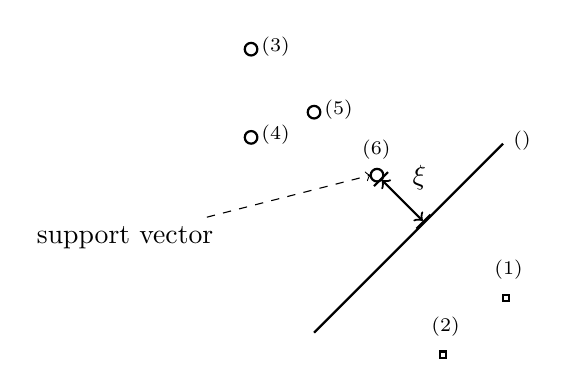
\begin{tikzpicture}[auto,scale=0.8]
					\draw [thick] (1,2) circle (0.1cm)node[anchor=west] {\hspace*{0mm}$\featurevec^{(5)}$};
					\draw [thick] (0,1.6) circle (0.1cm)node[anchor=west] {\hspace*{0mm}$\featurevec^{(4)}$};
					\draw [thick] (0,3) circle (0.1cm)node[anchor=west] {\hspace*{0mm}$\featurevec^{(3)}$};
					\draw [thick] (2,1) circle (0.1cm)node[anchor=east,above] {\hspace*{0mm}$\featurevec^{(6)}$};
					\node[] (B) at (-2,0) {support vector};
					\draw[->,dashed] (B) to (1.9,1) ; 
					\draw [|<->|,thick] (2.05,0.95)  -- (2.75,0.25)node[pos=0.5] {$\xi$} ; 
					\draw [thick] (1,-1.5) -- (4,1.5) node [right] {$\hypothesis^{(\weights)}$} ; 
					\draw [thick] (3,-1.9) rectangle ++(0.1cm,0.1cm) node[anchor=west,above]  {\hspace*{0mm}$\featurevec^{(2)}$};
					\draw [thick] (4,.-1) rectangle ++(0.1cm,0.1cm) node[anchor=west,above] {\hspace*{0mm}$\featurevec^{(1)}$};
				\end{tikzpicture}
				\caption{The SVM learns a \gls{hypothesis} (or \gls{classifier}) $\hypothesis^{(\weights)}$ with 
					minimal average soft-margin \gls{hingeloss}. Minimizing this \gls{loss} is equivalent 
					to maximizing the margin $\xi$ between the \gls{decisionboundary} of $\hypothesis^{(\weights)}$ 
					and each class of the \gls{trainset}.}
				\label{fig_svm_gls_dict}
			\end{center}
		\end{figure}
		The above basic variant of SVM is only useful if the \gls{datapoint}s from different categories can be  
		(approximately) linearly separated. For an \gls{ml} application where the categories are not 
		derived from a \gls{kernel}.\\
		\foreignlanguage{greek}{Βλέπε επίσης:} \gls{classification}, \gls{hypothesis}, \gls{map}, \gls{linreg}, \gls{logreg}, \gls{erm}, \gls{linmodel}, 
		\gls{lossfunc}, \gls{datapoint}, \gls{featurespace}, \gls{maximum}, \gls{hingeloss}, \gls{svm}, \gls{classifier}, \gls{loss}, \gls{decisionboundary}, 
		\gls{trainset}, \gls{ml}, \gls{kernel}.},
	first={\foreignlanguage{greek}{μηχανή διανυσμάτων υποστήριξης}},
	text={\foreignlanguage{greek}{μηχανή διανυσμάτων υποστήριξης}},
	user1={\foreignlanguage{greek}{μηχανή διανυσμάτων υποστήριξης}}, %nominative
	user2={\foreignlanguage{greek}{μηχανής διανυσμάτων υποστήριξης}}, %genitive
	user3={\foreignlanguage{greek}{μηχανή διανυσμάτων υποστήριξης}} %accusative    
}

\newglossaryentry{ml}
{name={\foreignlanguage{greek}{μηχανική μάθηση}},
	description={\foreignlanguage{greek}{Η μηχανική μάθηση}\index{\foreignlanguage{greek}{μηχανική μάθηση}} (machine learning - ML) 
		\foreignlanguage{greek}{στοχεύει να προβλέψει μία} \glsentryuseriii{label} \foreignlanguage{greek}{από τα} \glsentryuservi{feature} 
		\foreignlanguage{greek}{ενός} \glsentryuserii{datapoint}. \foreignlanguage{greek}{Οι μέθοδοι μηχανικής μάθησης το επιτυγχάνουν αυτό 
	 	μαθαίνοντας μία} \glsentryuseriii{hypothesis} \foreignlanguage{greek}{από έναν} \glsentryuseriii{hypospace} (\foreignlanguage{greek}{ή} \glsentryuseriii{model}) 
	 	\foreignlanguage{greek}{μέσω της ελαχιστο\-ποί\-ησης μίας} \glsentryuserii{lossfunc} \cite{MLBasics}, \cite{HastieWainwrightBook}. 
	 	\foreignlanguage{greek}{Μία ακριβής διατύπωση αυτής της αρχής είναι η} \glsentryuseri{erm}. \foreignlanguage{greek}{Διαφορετικές 
		μέθοδοι μηχανικής μάθησης προκύπτουν από διαφορετικές επιλογές σχεδιασμού για} \glsentryuservi{datapoint} (\foreignlanguage{greek}{δηλαδή 
		τα} \glsentryuservi{feature} \foreignlanguage{greek}{και την} \glsentryuseriii{label} \foreignlanguage{greek}{τους}), \foreignlanguage{greek}{το} 
	 	\glsentryuseriii{model}, \foreignlanguage{greek}{και τη} \glsentryuseriii{lossfunc} \cite[\foreignlanguage{greek}{Κεφ.} 3]{MLBasics}.\\
	 	\foreignlanguage{greek}{Βλέπε επίσης:} \gls{label}, \gls{feature}, \gls{datapoint}, \gls{hypothesis}, \gls{hypospace}, \gls{model}, \gls{lossfunc}, \gls{erm}.},
	first={ml},
	text={ml},
	user1={\foreignlanguage{greek}{μηχανική μάθηση}}, %nominative
	user2={\foreignlanguage{greek}{μηχανικής μά\-θη\-σης}}, %genitive  
	user3={\foreignlanguage{greek}{μηχανική μάθηση}} %accusative
} 

\newglossaryentry{model}
{name={\foreignlanguage{greek}{μοντέλο}}, 
	description={\foreignlanguage{greek}{Στο πλαίσιο της}\index{\foreignlanguage{greek}{μοντέλο}} \glsentryuserii{ml}, 
		\foreignlanguage{greek}{ο όρος μοντέλο συνήθως αναφέρεται στον υποκείμενο} \glsentryuseriii{hypospace}  
		\foreignlanguage{greek}{μίας μεθόδου} \glsentryuserii{ml} \cite{MLBasics}, \cite{ShalevMLBook}. 
		\foreignlanguage{greek}{Ωστόσο, ο όρος χρησιμοποιείται επίσης σε άλλα πεδία αλλά με διαφορετική σημασία. 
		Για παράδειγμα, ένα} \glsentryuseri{probmodel} \foreignlanguage{greek}{αναφέρεται σε ένα παραμετροποιημένο 
		σύνολο} \glsentryuserv{probdist}.\\
		\foreignlanguage{greek}{Βλέπε επίσης:} \gls{ml}, \gls{hypospace}, \gls{probmodel}, \gls{probdist}.},
	first={\foreignlanguage{greek}{μοντέλο}},
	text={mod\-el},
	user1={\foreignlanguage{greek}{μοντέλο}}, %nominative
	user2={\foreignlanguage{greek}{μοντέλου}}, %genitive
	user3={\foreignlanguage{greek}{μοντέλο}}, %accusative 
	user4={\foreignlanguage{greek}{μοντέλα}}, %nominativepl 
	user5={\foreignlanguage{greek}{μοντέλων}}, %genitivepl  
	user6={\foreignlanguage{greek}{μοντέλα}} %accusativepl 
}

\newglossaryentry{sbm}
{name={\foreignlanguage{greek}{μοντέλο στοχαστικής ομάδας}},
	description={\foreignlanguage{greek}{Το μοντέλο στοχαστικής ομάδας}\index{\foreignlanguage{greek}{μοντέλο στοχαστικής ομάδας}}
		(sto\-chastic block model - SBM) \foreignlanguage{greek}{είναι ένα πιθανοτικό παραγωγικό} \glsentryuseri{model} 
		\foreignlanguage{greek}{για έναν μη κατευθυνόμενο} \glsentryuseriii{graph} $\graph = \big( \nodes, \edges \big)$ 
		\foreignlanguage{greek}{με ένα δεδομένο σύνολο κόμβων} $\nodes$ \cite{AbbeSBM2018}. \foreignlanguage{greek}{Στην πιο 
		βασική του παραλλαγή, το μοντέλο στοχαστικής ομάδας παράγει έναν} \glsentryuseriii{graph} 
		\foreignlanguage{greek}{πρώτα αποδίδοντας τυχαία κάθε κόμβο $\nodeidx \in \nodes$ σε έναν δείκτη} 
		\glsentryuserii{cluster} $\clusteridx_{\nodeidx} \in \{1, \ldots, \nrcluster\}$. \foreignlanguage{greek}{Ένα ζεύγος διαφορετικών 
		κόμβων στον} \glsentryuseriii{graph} \foreignlanguage{greek}{συνδέεται με μία ακμή με} \glsentryuseriii{probability} $p_{\nodeidx,\nodeidx'}$ 
		\foreignlanguage{greek}{που εξαρτάται μόνο από τις} \glsentryuservi{label} $\clusteridx_{\nodeidx}, \clusteridx_{\nodeidx'}$. 
		\foreignlanguage{greek}{Η παρουσία ακμών μεταξύ διαφορετικών ζευγών κομβων είναι στατιστικά ανεξάρτητη.} \\
		\foreignlanguage{greek}{Βλέπε επίσης:} \gls{model}, \gls{graph}, \gls{cluster}, \gls{probability}, \gls{label}.},
	first={\foreignlanguage{greek}{μοντέλο στοχαστικής ομάδας}},
	text={\foreignlanguage{greek}{μοντέλο στοχαστικής ομάδας}},
	user1={\foreignlanguage{greek}{μοντέλο στοχαστικής ομάδας}}, %nominative
    	user2={\foreignlanguage{greek}{μοντέλου στοχαστικής ομάδας}} %genitive 
}

\newglossaryentry{lln}
{name={\foreignlanguage{greek}{νόμος των μεγάλων αριθμών}},
	description={\foreignlanguage{greek}{Ο νόμος των μεγάλων αριθ\-μών}\index{\foreignlanguage{greek}{νόμος των μεγάλων αριθμών}} 
		\foreignlanguage{greek}{αναφέρεται στη σύγκλιση του μέσου όρου ενός αυξανόμενου (μεγάλου) αριθ\-μού}  
		\glsentryuserii{iid} \glsentryuserv{rv} \foreignlanguage{greek}{στη} \glsentryuseriii{mean} \foreignlanguage{greek}{της κοινής τους} 
		\glsentryuserii{probdist}. \foreignlanguage{greek}{Διαφορετικές περιπτώσεις του νόμου των μεγάλων αριθμών προκύπτουν από 
		τη χρήση διαφορετικών εννοιών σύγκλισης} \cite{papoulis}.\\
		\foreignlanguage{greek}{Βλέπε επίσης:} \gls{iid}, \gls{rv}, \gls{mean}, \gls{probdist}.},
	first={\foreignlanguage{greek}{νόμος των μεγάλων αριθμών}},
	text={\foreignlanguage{greek}{νόμος των μεγάλων αριθμών}},
	user1={\foreignlanguage{greek}{νόμος των μεγάλων αριθμών}}, %nominative
	user2={\foreignlanguage{greek}{νόμου των μεγάλων αριθμών}} %genitive
}

\newglossaryentry{norm}
{name={\foreignlanguage{greek}{νόρμα}},
	description={\foreignlanguage{greek}{Μία νόρμα είναι μία}\index{\foreignlanguage{greek}{νόρμα}} \glsentryuseri{function} 
		\foreignlanguage{greek}{που αντιστοιχεί κάθε (διανυσματικό) στοιχείο ενός} \glsentryuserii{vectorspace} 
		\foreignlanguage{greek}{σε έναν μη αρνητικό αριθμό. Αυτή η} \glsentryuseri{function} \foreignlanguage{greek}{πρέπει 
		να είναι ομογενής και ορισμένη, και πρέπει να ικανοποιεί την τριγωνική ανισότητα} \cite{HornMatAnalysis}.\\
		\foreignlanguage{greek}{Βλέπε επίσης:} \gls{function}, \gls{vectorspace}. },
	first={\foreignlanguage{greek}{νόρμα}},
	text={\foreignlanguage{greek}{νόρμα}},
	user1={\foreignlanguage{greek}{νόρμα}}, %nominative
    	user2={\foreignlanguage{greek}{νόρμας}}, %genitive
	user3={\foreignlanguage{greek}{νόρμα}} %accusative 
}

\newglossaryentry{tv}
{name={\foreignlanguage{greek}{ολική μεταβολή}}, 
	description={\foreignlanguage{greek}{Βλέπε} \gls{gtv}\index{\foreignlanguage{greek}{ολική μεταβολή}}.},
	first={\foreignlanguage{greek}{ολική μεταβολή}},
	text={\foreignlanguage{greek}{ολική μεταβολή}},
	user1={\foreignlanguage{greek}{ολική μεταβολή}}, %nominative
	user2={\foreignlanguage{greek}{ολικής μεταβολής}} %genitive 
}

\newglossaryentry{rerm}
{name={\foreignlanguage{greek}{ομαλοποιημένη ελαχιστοποίηση εμπειρικής διακινδύνευσης}}, 
	description={Basic \gls{erm} learns a \gls{hypothesis} (or trains a \gls{model}) $\hypothesis \in \hypospace$ 
		based solely on the \gls{emprisk} $\emprisk{\hypothesis}{\dataset}$ incurred on a \gls{trainset} $\dataset$. 
		To make \gls{erm} less prone to \gls{overfitting}, we can implement \gls{regularization} by 
		including a (scaled) \gls{regularizer} $\regularizer{\hypothesis}$ in the learning objective. 
		This leads to RERM\index{\foreignlanguage{greek}{ομαλοποιημένη ελαχιστοποίηση εμπειρικής διακινδύνευσης}} 
		(regularized empirical risk minimization - RERM), 
		\begin{equation}
			\label{equ_def_rerm_dict}
			\learnthypothesis \in \aargmin_{\hypothesis \in \hypospace} \emprisk{\hypothesis}{\dataset} + \regparam \regularizer{\hypothesis}.
		\end{equation}
		The \gls{parameter} $\regparam \geq 0$ controls the \gls{regularization} strength. 
		For $\regparam = 0$, we recover standard \gls{erm} without \gls{regularization}. As $\regparam$ increases, the 
		learned \gls{hypothesis} is increasingly biased toward small values of $\regularizer{\hypothesis}$. 
		The component $\regparam \regularizer{\hypothesis}$ in the \gls{objfunc} of \eqref{equ_def_rerm_dict} 
		can be intuitively understood as a surrogate for the increased average \gls{loss} that may 
		occur when predicting \gls{label}s for \gls{datapoint}s outside the \gls{trainset}. This intuition  
		can be made precise in various ways. For example, consider a \gls{linmodel} trained using \gls{sqerrloss} 
		and the \gls{regularizer} $\regularizer{\hypothesis} = \normgeneric{\weights}{2}^{2}$. 
		In this setting, $\regparam \regularizer{\hypothesis}$ corresponds to the expected increase in \gls{loss} 
		caused by adding \gls{gaussrv}s to the \gls{featurevec}s in the \gls{trainset} 
		\cite[Ch. 3]{MLBasics}.
		A principled construction for the \gls{regularizer} $\regularizer{\hypothesis}$ 
		arises from approximate upper bounds on the \gls{generalization} error. The resulting 
		RERM instance is known as \gls{srm} \cite[Sec. 7.2]{ShalevShwartz2009}.\\
		\foreignlanguage{greek}{Βλέπε επίσης:} \gls{erm}, \gls{hypothesis}, \gls{model}, \gls{emprisk}, \gls{trainset}, \gls{overfitting}, 
		\gls{regularization}, \gls{regularizer}, \gls{parameter}, \gls{objfunc}, \gls{loss}, \gls{label}, \gls{datapoint}, \gls{linmodel}, \gls{sqerrloss}, 
		\gls{gaussrv}, \gls{featurevec}, \gls{generalization}, \gls{srm}.}, 
	first={\foreignlanguage{greek}{ομαλοποιημένη ελαχιστοποίηση εμπειρικής διακινδύνευσης}},
	text={\foreignlanguage{greek}{ομαλοποιημένη ελαχιστοποίηση εμπειρικής διακινδύνευσης}}, 
	user1={\foreignlanguage{greek}{ομαλοποιημένη ελαχιστοποίηση εμπειρικής διακινδύνευσης}}, %nominative
  	user2={\foreignlanguage{greek}{ομαλοποιημένης ελαχιστοποίησης εμπειρικής διακινδύνευσης}}, %genitive
	user3={\foreignlanguage{greek}{ομαλοποιημένη ελαχιστοποίηση εμπειρικής διακινδύνευσης}} %accusative 
}

\newglossaryentry{regularization}
{name={\foreignlanguage{greek}{ομαλοποίηση}}, 
	description={A\index{\foreignlanguage{greek}{ομαλοποίηση}} key challenge of modern \gls{ml} applications is that they often 
		use large \gls{model}s, which have an \gls{effdim} in the order of billions. 
		Training a high-dimensional \gls{model} using basic \gls{erm}-based methods
		is prone to \gls{overfitting}: the learned \gls{hypothesis} performs well on the \gls{trainset} 
		but poorly outside the \gls{trainset}. Regularization refers to modifications of a given instance 
		of \gls{erm} in order to avoid \gls{overfitting}, i.e., to ensure that the learned \gls{hypothesis} does 
		not perform much worse outside the \gls{trainset}. There are three routes for implementing 
		regularization: 
		\begin{enumerate}[label=\arabic*)]
			\item {\Gls{model} pruning:} We prune the original \gls{model} $\hypospace$ to obtain a 
			smaller \gls{model} $\hypospace'$. For a parametric \gls{model}, the pruning can be 
			implemented via constraints on the \gls{modelparams} (such as $w_{1} \in [0.4,0.6]$ for 
			the weight of \gls{feature} $x_{1}$ in \gls{linreg}).
			\item {\Gls{loss} penalization:} We modify the \gls{objfunc} of \gls{erm} by adding a 
			penalty term to the \gls{trainerr}. The penalty term estimates how much larger the expected \gls{loss} (or \gls{risk}) 
			is compared to the average \gls{loss} on the \gls{trainset}. 
			\item {\Gls{dataaug}:} We can enlarge the \gls{trainset} $\dataset$ by adding 
			perturbed copies of the original \gls{datapoint}s in $\dataset$. One example for such 
			a perturbation is to add the \gls{realization} of an \gls{rv} to the \gls{featurevec} 
			of a \gls{datapoint}. 
		\end{enumerate} 
		Fig. \ref{fig_equiv_dataaug_penal_dict} illustrates the above three routes to regularization. 
		These routes are closely related and sometimes fully equivalent: \gls{dataaug} using \gls{gaussrv}s 
		to perturb the \gls{featurevec}s in the \gls{trainset} of \gls{linreg} 
		has the same effect as adding the penalty 
		$\lambda \normgeneric{\weights}{2}^2$ to the \gls{trainerr} (which is nothing but \gls{ridgeregression}). 
        		The decision on which route to use for regularization can be based on the 
        		available computational infrastructure. For example, it might be much easier to 
       	 	implement \gls{dataaug} than \gls{model} pruning. 
		\begin{figure}[H]
			\begin{center} 
				\begin{tikzpicture}[scale = 1]
					% Axes
					\draw[->, very thick] (0,0.5) -- (7.7,0.5) node[right] {\gls{feature} $\feature$};       % X-axis
					\draw[->, very thick] (0.5,0) -- (0.5,4.2) node[above] {\gls{label} $\truelabel$};   % Y-axis
					\draw[color=black, thick, dashed, domain = -1: 6.2, variable = \x]  plot ({\x},{\x*0.4 + 2.0}) ;     
					\draw[color=black, thick, dashed, domain = -1: 6.2, variable = \x]  plot ({\x},{\x*0.6 + 2.0}) ;     
					% Add a lasso around the two dashed lines
	          			% Ellipse around the two dashed lines
					\draw[blue, thick] (5, 4.5) ellipse [x radius=0.2cm, y radius=1cm];
					\node at (5, 5.8) [text=black, font=\small] {$\{ \hypothesis: \hypothesis(x)\!=\!w_{1}x\!+\!w_{0}; w_{1} \in [0.4,0.6]\}$};
					\node at (6.7,4.5) {$\hypothesis(\feature)$};    
					\coordinate (l1)   at (1.2, 2.48);
					\coordinate (l2) at (1.4, 2.56);
					\coordinate (l3)   at (1.7,  2.68);
					\coordinate (l4)   at (2.2, 2.2*0.4+2.0);
					\coordinate (l5) at (2.4, 2.4*0.4+2.0);
					\coordinate (l6)   at (2.7,  2.7*0.4+2.0);
					\coordinate (l7)   at (3.9,  3.9*0.4+2.0);
					\coordinate (l8) at (4.2, 4.2*0.4+2.0);
					\coordinate (l9)   at (4.5,  4.5*0.4+2.0);
					\coordinate (n1)   at (1.2, 1.8);
					\coordinate (n2) at (1.4, 1.8);
					\coordinate (n3)   at (1.7,  1.8);
					\coordinate (n4)   at (2.2, 3.8);
					\coordinate (n5) at (2.4, 3.8);
					\coordinate (n6)   at (2.7,  3.8);
					% augemented data point obtained by perturbing feature, not touching label value 
					\coordinate (n7)   at (3.9, 2.6);
					\coordinate (n8) at (4.2, 2.6);
					\coordinate (n9)   at (4.5,  2.6);
					\node at (n1)  [circle,draw,fill=red,minimum size=6pt,scale=0.6, name=c1] {};
					\node at (n2)  [circle,draw,fill=blue,minimum size=6pt, scale=0.6, name=c2] {};
					\node at (n3)  [circle,draw,fill=red,minimum size=6pt,scale=0.6,  name=c3] {};
					\node at (n4)  [circle,draw,fill=red,minimum size=12pt, scale=0.6, name=c4] {};  
					\node at (n5)  [circle,draw,fill=blue,minimum size=12pt,scale=0.6,  name=c5] {};
					\node at (n6)  [circle,draw,fill=red,minimum size=12pt, scale=0.6, name=c6] {};  
					\node at (n7)  [circle,draw,fill=red,minimum size=12pt,scale=0.6,  name=c7] {};
					\node at (n8)  [circle,draw,fill=blue,minimum size=12pt, scale=0.6, name=c8] {};
					\node at (n9)  [circle,draw,fill=red,minimum size=12pt, scale=0.6, name=c9] {};
					\draw [<->] ($ (n7) + (0,-0.3) $)  --  ($ (n9) + (0,-0.3) $) node [pos=0.4, below] {$\sqrt{\regparam}$}; ; 
					\draw[<->, color=red, thick] (l1) -- (c1);  
					\draw[<->, color=blue, thick] (l2) -- (c2);  
					\draw[<->, color=red, thick] (l3) -- (c3);  
					\draw[<->, color=red, thick] (l4) -- (c4);  
					\draw[<->, color=blue, thick] (l5) -- (c5);  
					\draw[<->, color=red, thick] (l6) -- (c6);  
					\draw[<->, color=red, thick] (l7) -- (c7);  
					\draw[<->, color=blue, thick] (l8) -- (c8);  
					\draw[<->, color=red, thick] (l9) -- (c9);  
					\draw[fill=blue] (6.2, 3.7)  circle (0.1cm) node [black,xshift=2.3cm] {original \gls{trainset} $\dataset$};
					\draw[fill=red] (6.2, 3.2)  circle (0.1cm) node [black,xshift=1.3cm] {augmented};
					\node at (4.6,1.2)  [minimum size=12pt, font=\fontsize{12}{0}\selectfont, text=blue] {$\frac{1}{\samplesize} \sum_{\sampleidx=1}^\samplesize \lossfunc{\pair{\featurevec^{(\sampleidx)}}{ \truelabel^{(\sampleidx)}}}{\hypothesis}$};
					\node at (7.8,1.2)  [minimum size=12pt, font=\fontsize{12}{0}\selectfont, text=red] {$+\regparam \regularizer{\hypothesis}$};
				\end{tikzpicture}
				\caption{Three approaches to regularization: 1) \gls{dataaug}; 2) \gls{loss} penalization; and 3) \gls{model} 
				pruning (via constraints on \gls{modelparams}). \label{fig_equiv_dataaug_penal_dict} }
			\end{center}
		\end{figure} 
		\foreignlanguage{greek}{Βλέπε επίσης:} \gls{ml}, \gls{model}, \gls{effdim}, \gls{erm}, \gls{overfitting}, \gls{hypothesis}, \gls{trainset}, \gls{modelparams}, 
		\gls{feature}, \gls{linreg}, \gls{loss}, \gls{objfunc}, \gls{trainerr}, \gls{risk}, \gls{dataaug}, \gls{datapoint}, \gls{realization}, \gls{rv}, \gls{featurevec}, 
		\gls{gaussrv}, \gls{ridgeregression}, \gls{label}, \gls{validation}, \gls{modelsel}.},
	first={\foreignlanguage{greek}{ομαλοποίηση}},
	text={\foreignlanguage{greek}{ομαλοποίηση}},
	user1={\foreignlanguage{greek}{ομαλοποίηση}}, %nominative
	user2={\foreignlanguage{greek}{ομαλοποί\-ησης}} %genitive   
}

\newglossaryentry{regularizer}
{name={\foreignlanguage{greek}{ομαλοποιητής}}, 
	description={\foreignlanguage{greek}{Ένας ομαλοποιητής αποδίδει σε κάθε} \index{\foreignlanguage{greek}{ομαλοποιητής}} 
		\glsentryuseriii{hypothesis} $\hypothesis$ \foreignlanguage{greek}{από έναν} \glsentryuseriii{hypospace} $\hypospace$ 
		\foreignlanguage{greek}{ένα ποσοτικό μέτρο $\regularizer{\hypothesis}$ που εκφράζει σε ποιόν βαθμό τα σφάλματα} 
		\glsentryuserviii{prediction} \foreignlanguage{greek}{της μπορεί να διαφέρουν σε} \glsentryuservi{datapoint} 
		\foreignlanguage{greek}{σε ένα} \glsentryuseriii{trainset} \foreignlanguage{greek}{και έξω από αυτό. Η} 
		\glsentryuseri{ridgeregression} \foreignlanguage{greek}{χρησιμοποιεί τον ομαλοποιητή 
		$\regularizer{\hypothesis} \defeq \normgeneric{\weights}{2}^{2}$ για γραμμικές} \gls{map}s \glsentryuserii{hypothesis} 
		$\hypothesis^{(\weights)}(\featurevec) \defeq \weights\,^{T} \featurevec$ \cite[\foreignlanguage{greek}{Κεφ.} 3]{MLBasics}. 
		\foreignlanguage{greek}{Ο} \glsentryuseri{lasso} \foreignlanguage{greek}{χρησιμοποιεί τον ομαλοποιητή 
		$\regularizer{\hypothesis} \defeq \normgeneric{\weights}{1}$ για γραμμικές} \gls{map}s \glsentryuserii{hypothesis} 
		$\hypothesis^{(\weights)}(\featurevec) \defeq \weights\,^{T} \featurevec$ \cite[\foreignlanguage{greek}{Κεφ.} 3]{MLBasics}.\\
		\foreignlanguage{greek}{Βλέπε επίσης:} \gls{hypothesis}, \gls{hypospace}, \gls{prediction}, \gls{trainset}, \gls{datapoint}, 
		\gls{ridgeregression}, \gls{map}, \gls{lasso}.},
	first={\foreignlanguage{greek}{ομαλοποιητής}},
	text={\foreignlanguage{greek}{ομαλοποιητής}},
	user1={\foreignlanguage{greek}{ομαλοποιητής}}, %nominative
 	user2={\foreignlanguage{greek}{ομαλοποιητή}}, %genitive 
 	user3={\foreignlanguage{greek}{ομαλοποιητή}}, %accusative 
}

\newglossaryentry{fl}
{name={\foreignlanguage{greek}{ομοσπονδιακή μάθηση}}, 
	description={\foreignlanguage{greek}{Η ομοσπονδιακή μάθηση}\index{\foreignlanguage{greek}{ομοσπονδιακή μάθηση}} 
		(federated learning - FL) \foreignlanguage{greek}{είναι ένας όρος-ομπρέλα για μεθόδους} \glsentryuserii{ml} 
		\foreignlanguage{greek}{που εκπαι\-δεύ\-ουν} \glsentryuservi{model} \foreignlanguage{greek}{με έναν συνεργατικό
		τρόπο χρησιμοποιώντας αποκεντρωμένα} \glsentryuseriii{data} \foreignlanguage{greek}{και υπολογισμό}.\\
		\foreignlanguage{greek}{Βλέπε επίσης:} \gls{ml}, \gls{model}, \gls{data}.},
	first={federated learning (FL)},
	text={FL}, 
	user1={\foreignlanguage{greek}{ομοσπονδιακή μάθηση}}, %nominative
  	user2={\foreignlanguage{greek}{ομοσπονδιακής μάθησης}} %genitive 
}

\newglossaryentry{hfl}
{name={\foreignlanguage{greek}{οριζόντια ομοσπονδιακή μάθηση}},
	description={\foreignlanguage{greek}{Η οριζόντια ομοσπονδιακή μάθηση}\index{\foreignlanguage{greek}{οριζόντια ομοσπονδιακή μάθηση}}\linebreak 
		(horizontal federated learning - HFL) \foreignlanguage{greek}{χρησιμοποιεί} \glsentryuservi{localdataset} \foreignlanguage{greek}{που 
		αποτελούνται από διαφορετικά} \glsentryuservi{datapoint}, \foreignlanguage{greek}{αλλά χρησιμοποιεί τα ίδια} \glsentryuservi{feature} 
		\foreignlanguage{greek}{για να τα χαρακτηρίσει} \cite{HFLChapter2020}. \foreignlanguage{greek}{Για παράδειγμα, η πρόγνωση 
		καιρού χρησιμοποιεί ένα δίκτυο χωρικά κατανεμημένων σταθμών (παρατήρησης) καιρού. Κάθε σταθμός καιρού 
		μετράει τις ίδιες ποσότητες, όπως την ημερήσια θερμοκρασία, την ατμοσφαιρική πίεση, και τα ατμοσφαιρικά κατακρημνίσματα.
		Ωστόσο, διαφορετικοί σταθ\-μοί καιρού μετράνε τα} characteristics \foreignlanguage{greek}{ή τα}
		\glsentryuservi{feature} \foreignlanguage{greek}{διαφορετικών χωροχρονικών περιοχών. Κάθε χωροχρονική περιοχή
		αναπαριστά ένα μεμονωμένο} \glsentryuseriii{datapoint}, \foreignlanguage{greek}{με το καθένα να χαρακτηρίζεται από τα ίδια} 
		\glsentryuservi{feature} \foreignlanguage{greek}{(δηλαδή ημερήσια θερμοκρασία ή ατμοσφαιρική πίεση).} \\
		\foreignlanguage{greek}{Βλέπε επίσης:} \gls{localdataset}, \gls{datapoint}, \gls{feature}, \gls{ssl}, \gls{fl}, \gls{vfl}.},
	first={\foreignlanguage{greek}{οριζόντια ομοσπονδιακή μάθηση}},
	text={\foreignlanguage{greek}{οριζόντια ομοσπονδιακή μάθηση}},
	user1={\foreignlanguage{greek}{οριζόντια ομοσπονδιακή μάθηση}}, %nominative
	user2={\foreignlanguage{greek}{οριζόντιας ομοσπονδιακής μάθησης}} %genitive 
} 

\newglossaryentry{det}
{name={\foreignlanguage{greek}{ορίζουσα}},
	description={The\index{\foreignlanguage{greek}{ορίζουσα}} determinant $\det\,(\mA)$ of a square matrix 
		$\mA = \big( \va^{(1)},\ldots, \va^{(\nrfeatures)} \big) \in \mathbb{R}^{\nrfeatures \times \nrfeatures}$ is a 
		\gls{function} of its columns $\va^{(1)},\ldots,\va^{(\nrfeatures)} \in \mathbb{R}^{\nrfeatures}$, that is \cite{DirschmidHansJorg1996TuF}
		\begin{itemize}
			\item Normalized: $$\det (\mI) = 1$$ 
			\item Multi-linear: \begin{align} \nonumber \det \big(\va^{(1)},\ldots,\alpha\vu+ \beta \vv,\ldots,\va^{(\nrfeatures)} \big) & = \alpha\det \big(\va^{(1)},\ldots,\vu,\ldots,\va^{(\nrfeatures)} \big) \\ 
			& +\beta\det \big(\va^{(1)},\ldots,\vv,\ldots,\va^{(\nrfeatures)} \big) \nonumber
			\end{align}
			\item Anti-symmetric: $$\det \big(\ldots,\va^{(\featureidx)}, \ldots, \va^{(\featureidx')},\ldots \big) = - \det \big(\ldots,\va^{(\featureidx')}, \ldots, \va^{(\featureidx)},\ldots \big).$$ 
		\end{itemize} 
		We can interpret a matrix $\mA$ as a linear transformation on $\mathbb{R}^{\nrfeatures}$.
		The determinant $\det\,(\mA)$ characterizes how (the orientation of) 
 		volumes in $\mathbb{R}^\nrfeatures$ are altered by this transformation \cite{GolubVanLoanBook}, \cite{Strang2007}. 
 		In particular, $\det\,(\mA) > 0$ preserves orientation, $\det\,(\mA) < 0$ reverses orientation, 
 		and $\det\,(\mA) = 0$ collapses volume entirely, indicating that $\mA$ is non-invertible. 
 		The determinant also satisfies $\det\,(\mA \mB) = \det\,(\mA) \cdot \det\,(\mB)$, and if $\mA$ is 
 		diagonalizable with \gls{eigenvalue}s $\eigval{1}, \ldots, \eigval{\nrfeatures}$, then 
		$\det(\mA) = \prod_{\featureidx=1}^{\nrfeatures} \eigval{\featureidx}$ \cite{HornMatAnalysis}.
    		For the special cases $\nrfeatures=2$ (2D) and $\nrfeatures=3$ (3D), the determinant can be 
		interpreted as an oriented area or volume spanned by the column vectors of $\mA$.
    		\begin{figure}[H]
    			\begin{center}
    			\begin{tikzpicture}[x=2cm]
			% LEFT: Standard basis vectors and unit square
			\begin{scope}
			\draw[->, thick] (0,0) -- (1,0) node[below right] {$\vx$};
			\draw[->, thick] (0,0) -- (0,1) node[above left] {$\vy$};
			%\draw[fill=gray!15] (0,0) -- (1,0) -- (1,1) -- (0,1) -- cycle;
			%\node at (0.5,0.5) {\small unit square};
			%\node at (0.5,-0.6) {standard basis};
			\end{scope}
			% RIGHT: Transformed basis vectors and parallelogram
			\begin{scope}[shift={(2.8,0)}]
			\coordinate (A) at (1.5,0.5);
			\coordinate (B) at (-0.2,1.2);
			\draw[->, very thick, red] (0,0) -- (A) node[below right] {$\mA \vx$};
			\draw[->, very thick, red] (0,0) -- (B) node[above left] {$\mA \vy$};
			\draw[fill=red!20, opacity=0.6] (0,0) -- (A) -- ($(A)+(B)$) -- (B) -- cycle;
			\draw[dashed] (A) -- ($(A)+(B)$);
			\draw[dashed] (B) -- ($(A)+(B)$);
			\node at (0.8,0.6) {\small $\det\,(\mA)$};
			% Orientation arc
			\draw[->, thick, blue] (0.4,0.0) arc[start angle=0, end angle=35, radius=0.6];
			%	\node[blue] at (0.25,1.25) {};
			%	\node at (0.8,-0.6) {transformed basis};
			\end{scope}
			% Arrow between plots
			\draw[->, thick] (1.3,0.5) -- (2.4,0.5) node[midway, above] {$\mA$};
			\end{tikzpicture}
			\end{center}
			\caption{We can interpret a square \gls{matrix} $\mA$ as a linear transformation of $\mathbb{R}^{\nrfeatures}$ 
				into itself. The determinant $\det\,(\mA)$ characterizes how this transformation alters an oriented volume.}
		\end{figure}
		\foreignlanguage{greek}{Βλέπε επίσης:} \gls{function}, \gls{eigenvalue}, \gls{matrix}, \gls{inverse}.},
	first={\foreignlanguage{greek}{ορίζουσα}},
	text={\foreignlanguage{greek}{ορίζουσα}},
	user1={\foreignlanguage{greek}{ορίζουσα}}, %nominative 
	user2={\foreignlanguage{greek}{ορίζουσας}}, %genitive 
	user3={\foreignlanguage{greek}{ορίζουσα}}, %accusative 
	user4={\foreignlanguage{greek}{ορίζουσά}} %nominativeoraccusativedoublestress 
}

\newglossaryentry{decisionboundary}
{name={\foreignlanguage{greek}{όριο απόφασης}}, 
	description={\foreignlanguage{greek}{Θεωρούμε μία}\index{\foreignlanguage{greek}{όριο απόφασης}}  
		\gls{map} \glsentryuserii{hypothesis} $\hypothesis$ \foreignlanguage{greek}{που διαβάζει ένα} \glsentryuseriii{featurevec}  
		$\featurevec \in \mathbb{R}^{\featuredim}$ \foreignlanguage{greek}{και παραδίδει μία τιμή από ένα πεπερασμένο σύνολο $\labelspace$. 
		Το όριο απόφασης της $\hypothesis$ είναι το σύνολο των διανυσμάτων $\featurevec \in \mathbb{R}^{\featuredim}$ 
		που βρίσκονται ανάμεσα σε διαφορετικές} \glsentryuservi{decisionregion}. \foreignlanguage{greek}{Πιο συγκεκριμένα, ένα  
		διάνυσμα $\featurevec$ ανήκει στο όριο απόφασης αν και μόνο αν κάθε} \glsentryuseri{neighborhood} 
		$\{ \featurevec': \| \featurevec - \featurevec' \| \leq \varepsilon \}$, \foreignlanguage{greek}{για οποιοδήποτε $\varepsilon >0$, περιέχει 
		τουλάχιστον δύο διανύσματα με διαφορετικές τιμές} \glsentryuserii{function}.\\
		\foreignlanguage{greek}{Βλέπε επίσης:} \gls{hypothesis}, \gls{map}, \gls{featurevec}, \gls{decisionregion}, \gls{neighborhood}, \gls{function}.},
	first={\foreignlanguage{greek}{όριο απόφασης}},
	text={\foreignlanguage{greek}{όριο απόφασης}},
	user1={\foreignlanguage{greek}{όριο απόφασης}}, %nominative
	user2={\foreignlanguage{greek}{ορίου απόφασης}}, %genitive 
	user3={\foreignlanguage{greek}{ορίο απόφασης}} %accusative 
}

\newglossaryentry{regression}
{name={\foreignlanguage{greek}{παλινδρόμηση}},
	description={\foreignlanguage{greek}{Τα προβλήματα παλινδρόμησης}\index{\foreignlanguage{greek}{παλινδρόμηση}} 
		\foreignlanguage{greek}{περιστρέφονται γύρω από την}  
		\glsentryuseriii{prediction} \foreignlanguage{greek}{μίας αριθμητικής} \glsentryuserii{label} \foreignlanguage{greek}{μόνο από τα} 
		\glsentryuservi{feature} \foreignlanguage{greek}{ενός} \glsentryuserii{datapoint} \cite[\foreignlanguage{greek}{Κεφ.} 2]{MLBasics}.\\
		\foreignlanguage{greek}{Βλέπε επίσης:} \gls{prediction}, \gls{label}, \gls{feature}, \gls{datapoint}.},
	first={regression},
	text={regression},
	user1={\foreignlanguage{greek}{παλινδρόμηση}}, %nominative
  	user2={\foreignlanguage{greek}{παλινδρόμησης}} %genitive
}

\newglossaryentry{ladregression}
{name={\foreignlanguage{greek}{παλινδρόμηση ελάχιστης απόλυτης απόκλισης}},
	description={\foreignlanguage{greek}{Η παλινδρόμηση ελά\-χιστης απόλυτης 
		απόκλισης}\index{\foreignlanguage{greek}{παλινδρόμηση ελάχιστης απόλυτης απόκλισης}} 
		\foreignlanguage{greek}{είναι μία περίπτωση της} \glsentryuserii{erm} \foreignlanguage{greek}{που 
		χρησιμοποιεί την} \glsentryuseriii{abserr}. \foreignlanguage{greek}{Είναι μία ειδική περίπτωση της} 
		\glsentryuserii{huberreg}.\\
		\foreignlanguage{greek}{Βλέπε επίσης:} \gls{erm}, \gls{abserr}, \gls{huberreg}.},
	first={\foreignlanguage{greek}{παλινδρόμηση ελάχιστης απόλυτης απόκλισης}},
	text={\foreignlanguage{greek}{παλινδρόμηση ελάχιστης απόλυτης απόκλισης}},
	user1={\foreignlanguage{greek}{παλινδρόμηση ελάχιστης απόλυτης απόκλισης}}, %nominative
	user2={\foreignlanguage{greek}{παλινδρόμησης ελάχιστης απόλυτης απόκλισης}} %genitive  
}

\newglossaryentry{huberreg}
{name={\foreignlanguage{greek}{παλινδρόμηση} Huber},
	description={\foreignlanguage{greek}{Η} \glsentryuseri{regression} Huber\index{\foreignlanguage{greek}{παλινδρόμηση} Huber} 
		\foreignlanguage{greek}{αναφέρεται σε μεθόδους βασισμένες στην} \glsentryuseriii{erm} 
		\foreignlanguage{greek}{που χρησιμοποιούν την} \glsentryuseriii{huberloss} \foreignlanguage{greek}{ως μέτρο του σφάλματος} 
		\glsentryuserii{prediction}. \foreignlanguage{greek}{Δύο σημαντικές ειδικές περιπτώσεις της} \glsentryuserii{regression} Huber 
		\foreignlanguage{greek}{είναι η} \glsentryuseri{ladregression} \foreignlanguage{greek}{και η} \glsentryuseri{linreg}. 
		\foreignlanguage{greek}{Η ρύθμιση της} \glsentryuserii{parameter}-\foreignlanguage{greek}{κατωφλιού 
		της} \glsentryuserii{huberloss} \foreignlanguage{greek}{επιτρέπει στον χρήστη να ανταλλάξει την} \glsentryuseriii{robustness} 
		\foreignlanguage{greek}{της} \glsentryuserii{abserr} 
		\foreignlanguage{greek}{με τα υπολογιστικά οφέλη της} \glsentryuserii{smooth} \glsentryuserii{sqerrloss}.\\
		\foreignlanguage{greek}{Βλέπε επίσης:} \gls{regression}, \gls{erm}, \gls{huberloss}, \gls{prediction}, \gls{regression}, \gls{ladregression}, 
		\gls{linreg}, \gls{parameter}, \gls{robustness}, \gls{abserr}, \gls{smooth}, \gls{sqerrloss}.},
	first={\foreignlanguage{greek}{παλινδρόμηση} Huber},
	text={\foreignlanguage{greek}{παλινδρόμηση} Huber},
	user1={\foreignlanguage{greek}{παλινδρόμηση} Huber}, %nominative
	user2={\foreignlanguage{greek}{παλινδρόμησης} Huber} %genitive  
}

\newglossaryentry{differentiable}
{name={\foreignlanguage{greek}{παραγωγίσιμη}},
	description={\foreignlanguage{greek}{Μία} \glsentryuseri{function} \foreignlanguage{greek}{πραγματικής 
		τιμής}\index{\foreignlanguage{greek}{παραγωγίσιμη}} $f: \mathbb{R}^{\featuredim} \rightarrow \mathbb{R}$ 
		\foreignlanguage{greek}{είναι παραγωγίσιμη αν μπορεί να προσεγγιστεί τοπικά σε οποιοδήποτε σημείο από μία  
		γραμμική} \glsentryuseriii{function}. \foreignlanguage{greek}{Η τοπική γραμμική προσέγγιση στο σημείο $\mathbf{x}$ καθορίζεται
		από την} \glsentryuseriii{gradient} $\nabla f ( \mathbf{x})$ \cite{RudinBookPrinciplesMatheAnalysis}.\\
		\foreignlanguage{greek}{Βλέπε επίσης:} \gls{function}, \gls{gradient}.},
	first={\foreignlanguage{greek}{παραγωγίσιμη}},
	text={\foreignlanguage{greek}{παραγωγίσιμη}},
	user1={\foreignlanguage{greek}{παραγωγίσιμη}}, %nominative
  	user2={\foreignlanguage{greek}{παραγωγίσιμης}} %genitive   
}

\newglossaryentry{iidasspt}
{name={\foreignlanguage{greek}{παραδοχή ανεξάρτητων και ταυτόσημα κατανεμημένων}}, 
	description={\foreignlanguage{greek}{Η παραδοχή} \glsentryuserii{iid}\index{\foreignlanguage{greek}{παραδοχή ανεξάρτητων και ταυτόσημα κατανεμημένων}} 
		(independent and identically distributed assumption - i.i.d.\ assumption) \foreignlanguage{greek}{ερμηνεύει} \glsentryuservi{datapoint} 
		\foreignlanguage{greek}{ενός} \glsentryuserii{dataset} \foreignlanguage{greek}{ως τις} \glsentryuservi{realization} \glsentryuserii{iid} \glsentryuserv{rv}.\\
		\foreignlanguage{greek}{Βλέπε επίσης:} \gls{iid}, \gls{datapoint}, \gls{dataset}, \gls{realization}, \gls{rv}.},
	first={\foreignlanguage{greek}{παραδοχή ανεξάρτητων και ταυτόσημα κατανεμημένων}},
	text={\foreignlanguage{greek}{παραδοχή ανεξάρτητων και ταυτόσημα κατανεμημένων}},
	user1={\foreignlanguage{greek}{παραδοχή ανεξάρτητων και ταυτόσημα κατανεμημένων}}, %nominative
  	user2={\foreignlanguage{greek}{παραδοχής ανεξάρτητων και ταυτόσημα κατανεμημένων}}, %genitive   
	user3={\foreignlanguage{greek}{παραδοχή ανεξάρτητων και ταυτόσημα κατανεμημένων}} %accusative  
}

\newglossaryentry{clustasspt}
{name={\foreignlanguage{greek}{παραδοχή συσταδοποίησης}}, 
	description={\foreignlanguage{greek}{Η παραδοχή}\index{\foreignlanguage{greek}{παραδοχή συσταδοποίησης}} 
		\glsentryuserii{clustering} \foreignlanguage{greek}{υποθέτει ότι} \glsentryuseriv{datapoint} \foreignlanguage{greek}{σε 
		ένα} \glsentryuseriii{dataset} \foreignlanguage{greek}{σχηματίζουν έναν (μικρό) αριθμό ομάδων ή} \glsentryuserv{cluster}. 
		\foreignlanguage{greek}{Τα} \glsentryuseriv{datapoint} \foreignlanguage{greek}{στην ίδια} \glsentryuseriii{cluster} 
		\foreignlanguage{greek}{είναι πιο όμοια μεταξύ τους παρά με αυτά εκτός της} \glsentryuserii{cluster} 
		\cite{SemiSupervisedBook}. \foreignlanguage{greek}{Αποκτούμε διαφορετικές μεθόδους} \glsentryuserii{clustering} 
		\foreignlanguage{greek}{χρησιμοποιώντας διαφορετικές έννοιες ομοιότητας ανάμεσα σε} \glsentryuservi{datapoint}.\\
		\foreignlanguage{greek}{Βλέπε επίσης:} \gls{clustering}, \gls{datapoint}, \gls{dataset}, \gls{cluster}.},
	first={\foreignlanguage{greek}{παραδοχή συσταδοποίησης}},
	text={\foreignlanguage{greek}{παραδοχή συσταδοποίησης}},
	user1={\foreignlanguage{greek}{παραδοχή συσταδοποίησης}}, %nominative
	user2={\foreignlanguage{greek}{παραδοχής συσταδοποίησης}} %genitive 
}

\newglossaryentry{parameter}
{name={\foreignlanguage{greek}{παράμετρος}},
	description={\foreignlanguage{greek}{Η παράμετρος ενός}\index{\foreignlanguage{greek}{παράμετροι}} \glsentryuserii{model} \glsentryuserii{ml} 
		\foreignlanguage{greek}{είναι μία ποσότητα που μπορεί να ρυθμιστεί (δηλαδή να μαθευτεί ή να προσαρμοστεί) και που μας επιτρέπει 
		να επιλέξουμε μεταξύ διαφορετικών} \gls{map}s \glsentryuserii{hypothesis}. \foreignlanguage{greek}{Για παράδειγμα, το} \glsentryuseri{linmodel} 
		$\hypospace \defeq \{\hypothesis^{(\weights)}: \hypothesis^{(\weights)}(\feature)= \weight_{1} \feature + \weight_{2}\}$ 
		\foreignlanguage{greek}{αποτελείται από όλες τις} \gls{map}s \glsentryuserii{hypothesis} $\hypothesis^{(\weights)}(\feature)= \weight_{1} \feature + \weight_{2}$ 
		\foreignlanguage{greek}{με μία συγκεκριμένη επιλογή για τις παραμέτρους $\weights = \big(\weight_{1},\weight_{2}\big)\,^{T} \in \mathbb{R}^{2}$. 
		Ένα άλλο παράδειγμα μίας παραμέτρου} \glsentryuserii{model} \foreignlanguage{greek}{είναι τα} \glsentryuseri{weights} 
		\foreignlanguage{greek}{που αποδίδονται σε μία σύνδεση μεταξύ δύο νευρώνων ενός} \glsentryuserii{ann}.\\
		\foreignlanguage{greek}{Βλέπε επίσης:} \gls{ml}, \gls{model}, \gls{hypothesis}, \gls{map}, \gls{linmodel}, \gls{weights}, \gls{ann}.},
	first={\foreignlanguage{greek}{παράμετρος}},
	text={\foreignlanguage{greek}{παράμετρος}},
	user1={\foreignlanguage{greek}{παράμετρος}}, %nominative
	user2={\foreignlanguage{greek}{παραμέτρου}}, %genitive
	user3={\foreignlanguage{greek}{παράμετρο}}, %accusative
	user4={\foreignlanguage{greek}{παράμετροι}}, %nominativepl
	user5={\foreignlanguage{greek}{παραμέτρων}}, %genitivepl
	user6={\foreignlanguage{greek}{παραμέτρους}}, %accusativepl
	user7={\foreignlanguage{greek}{παραμετρικό}} %nominativeoraccusativeneutadj
}

\newglossaryentry{modelparams}
{name={\foreignlanguage{greek}{παράμετροι μοντέλου}}, 
	description={\foreignlanguage{greek}{Οι} \glsentryuseriv{parameter} \glsentryuserii{model}\index{\foreignlanguage{greek}{παράμετροι μοντέλου}} 
		\foreignlanguage{greek}{είναι ποσότητες που χρησιμοποιούνται για να επιλεχθεί μία συγκεκριμένη} \gls{map}  
		\glsentryuserii{hypothesis} \foreignlanguage{greek}{από ένα} \glsentryuseriii{model}. 
		\foreignlanguage{greek}{Μπορούμε να σκεφτούμε μία λίστα} \glsentryuserv{parameter} \glsentryuserii{model} 
		\foreignlanguage{greek}{ως ένα μοναδικό αναγνωριστικό για μία} \gls{map} \glsentryuserii{hypothesis} 
		\foreignlanguage{greek}{όμοια με το πώς ένας αριθμός κοινωνικής ασφάλισης ταυτοποιεί ένα άτομο στην Ελλάδα.} \\
		\foreignlanguage{greek}{Βλέπε επίσης:} \gls{model}, \gls{parameter}, \gls{hypothesis}, \gls{map}.},
	first={\foreignlanguage{greek}{παράμετροι μοντέλου}},
	text={\foreignlanguage{greek}{παράμετροι μοντέλου}},
	user1={\foreignlanguage{greek}{παράμετροι μοντέλου}}, %nominativepl
	user2={\foreignlanguage{greek}{παραμέτρων μοντέλου}}, %genitivepl
	user3={\foreignlanguage{greek}{παραμέτρους μοντέλου}}, %accusativepl 
	user4={\foreignlanguage{greek}{παράμετροι του μοντέλου}}, %nominativeplart
	user5={\foreignlanguage{greek}{παραμέτρων του μοντέλου}}, %genitiveplart
	user6={\foreignlanguage{greek}{παραμέτρους του μοντέλου}} %accusativeplart 
}

\newglossaryentry{decisionregion}
{name={\foreignlanguage{greek}{περιοχή αποφάσεων}}, 
	description={\foreignlanguage{greek}{Θεωρούμε μία} \gls{map}\index{\foreignlanguage{greek}{περιοχή αποφάσεων}} 
		\glsentryuserii{hypothesis} $\hypothesis$ \foreignlanguage{greek}{που δίνει τιμές από ένα πεπερασμένο σύνολο $\labelspace$. 
		Για κάθε τιμή} \glsentryuserii{label} \foreignlanguage{greek}{(δηλαδή κατηγορία) $a \in \labelspace$, η} \glsentryuseri{hypothesis} $\hypothesis$ 
		\foreignlanguage{greek}{καθορίζει ένα υποσύνολο τιμών} \glsentryuserv{feature} $\featurevec \in \featurespace$ \foreignlanguage{greek}{που  
		οδηγούν στις ίδιες εξόδους $\hypothesis(\featurevec)=a$. Αναφερόμαστε σε αυτό το υποσύνολο ως μία περιοχή αποφάσεων  
		της} \glsentryuserii{hypothesis} $\hypothesis$.\\
		\foreignlanguage{greek}{Βλέπε επίσης:} \gls{hypothesis}, \gls{map}, \gls{label}, \gls{feature}.},
	first={\foreignlanguage{greek}{περιοχή αποφάσεων}},
	text={\foreignlanguage{greek}{περιοχή αποφάσεων}},
	user1={\foreignlanguage{greek}{περιοχή αποφάσεων}}, %nominative
	user2={\foreignlanguage{greek}{περιοχής αποφάσεων}}, %genitive  
	user3={\foreignlanguage{greek}{περιοχή αποφάσεων}}, %accusative
	user4={\foreignlanguage{greek}{περιοχές αποφάσεων}}, %nominativepl
	user5={\foreignlanguage{greek}{περιοχών αποφάσεων}}, %genitivepl
	user6={\foreignlanguage{greek}{περιοχές αποφάσεων}} %accusativepl
}

\newglossaryentry{probability}
{name={\foreignlanguage{greek}{πιθανότητα}},
	description={\foreignlanguage{greek}{Αποδίδουμε}\index{\foreignlanguage{greek}{πιθανότητα}} \foreignlanguage{greek}{μία τιμή 
		πιθανότητας, συνήθως επιλεγμένη στο διάστημα $[0,1]$, σε κάθε γεγονός που μπορεί να συμβεί σε ένα τυχαίο 
		πεί\-ραμα} \cite{BillingsleyProbMeasure}, \cite{BertsekasProb}, \cite{HalmosMeasure}, \cite{KallenbergBook}.},
	first={probability},
	text={probability},
	user1={\foreignlanguage{greek}{πιθανότητα}}, %nominative
    	user2={\foreignlanguage{greek}{πιθανότητας}}, %genitive 
	user3={\foreignlanguage{greek}{πιθανότητα}}, %accusative 
	user4={\foreignlanguage{greek}{πιθανότητες}}, %nominativepl
    	user5={\foreignlanguage{greek}{πιθανοτήτων}}, %genitivepl 
	user6={\foreignlanguage{greek}{πιθανότητες}} %accusativepl 
}

\newglossaryentry{probmodel}
{name={\foreignlanguage{greek}{πιθανοτικό μοντέλο}},
	description={\foreignlanguage{greek}{Ένα πιθανοτικό} \glsentryuseri{model}\index{\foreignlanguage{greek}{πιθανοτικό μοντέλο}} 
		\foreignlanguage{greek}{ερμηνεύει} \glsentryuservi{datapoint} \foreignlanguage{greek}{ως}
		\glsentryuservi{realization} \glsentryuserv{rv} \foreignlanguage{greek}{με κοινή} \glsentryuseriii{probdist}. \foreignlanguage{greek}{Αυτή η κοινή} 
		\glsentryuseri{probdist} \foreignlanguage{greek}{συνήθως περιλαμβάνει} 
		\glsentryuservi{parameter} \foreignlanguage{greek}{που πρέπει να επιλεχθούν χειρωνακτικά ή να μαθευτούν μέσω μεθόδων στατιστικής  
		συμπερασματολογίας όπως η εκτίμηση} \glsentryuserii{maxlikelihood}  \cite{LC}.\\
		\foreignlanguage{greek}{Βλέπε επίσης:} \gls{model}, \gls{datapoint}, \gls{realization}, \gls{rv}, \gls{probdist}, \gls{parameter}, \gls{maxlikelihood}.}, 
	first={\foreignlanguage{greek}{πιθανοτικό μοντέλο}}, 
	text={\foreignlanguage{greek}{πιθανοτικό μοντέλο}},
	user1={\foreignlanguage{greek}{πιθανοτικό μοντέλο}}, %nominative
   	user2={\foreignlanguage{greek}{πιθανοτικού μοντέλου}}, %genitive    
	user3={\foreignlanguage{greek}{πιθανοτικό μοντέλο}}, %accusative 
	user4={\foreignlanguage{greek}{πιθανοτικά μοντέλα}}, %nominativepl
   	user5={\foreignlanguage{greek}{πιθανοτικών μοντέλων}}, %genitivepl 
	user6={\foreignlanguage{greek}{πιθανοτικά μοντέλα}} %accusativepl 
}

\newglossaryentry{cm}
{name={\foreignlanguage{greek}{πίνακας σύγχυσης}}, 
	description={\foreignlanguage{greek}{Θεωρούμε}\index{\foreignlanguage{greek}{πίνακας σύγχυσης}} \glsentryuservi{datapoint}  
		\foreignlanguage{greek}{που χαρακτηρίζονται από} \glsentryuservi{feature} $\featurevec$ \foreignlanguage{greek}{και 
		αντίστοιχες} \glsentryuservi{label} $\truelabel$. \foreignlanguage{greek}{Οι} \glsentryuseriv{label}  
		\foreignlanguage{greek}{παίρνουν τιμές σε έναν πεπερασμένο} \glsentryuseriii{labelspace} $\labelspace = \{1, \ldots, \nrcluster\}$. 
		\foreignlanguage{greek}{Για μία δεδομένη} \glsentryuseriii{hypothesis} $\hypothesis$, \foreignlanguage{greek}{ο πίνακας σύγχυσης 
		είναι ένας $\nrcluster \times \nrcluster$ πίνακας όπου κάθε γραμμή αντιστοιχεί σε μία διαφορετική τιμή της αληθούς} 
		\glsentryuserii{label} $\truelabel \in \labelspace$ \foreignlanguage{greek}{και κάθε στήλη σε μία διαφορετική τιμή της}  
		\glsentryuserii{prediction} $\hypothesis(\featurevec) \in \labelspace$. \foreignlanguage{greek}{Η $(\clusteridx,\clusteridx')$-στή 
		καταχώριση του πίνακα σύγχυσης αναπαριστά το κλάσμα των} \glsentryuserv{datapoint} \foreignlanguage{greek}{με μία 
		πραγματική} \glsentryuseriii{label} $\truelabel = \clusteridx$ \foreignlanguage{greek}{που προβλέπονται ως  
		$\hypothesis(\featurevec) = \clusteridx'$. Η κύρια διαγώνιος του πίνακα σύγχυσης περιέχει τα κλάσματα των σωστά ταξινομημένων}
		\glsentryuserv{datapoint} (\foreignlanguage{greek}{δηλαδή αυτών για τα οποία $\truelabel = \hypothesis(\featurevec)$). Οι 
		εκτός διαγωνίου καταχωρίσεις περιέχουν τα κλάσματα των} \glsentryuserv{datapoint} \foreignlanguage{greek}{που είναι 
		εσφαλμένα ταξινομημένα από την} $\hypothesis$. \\
		\foreignlanguage{greek}{Βλέπε επίσης:} \gls{datapoint}, \gls{feature}, \gls{label}, \gls{labelspace}, \gls{hypothesis}, \gls{prediction}, \gls{classification}. },
	first={\foreignlanguage{greek}{πίνακας σύγχυσης}},
	text={\foreignlanguage{greek}{πίνακας σύγχυσης}},
	user1={\foreignlanguage{greek}{πίνακας σύγχυσης}}, %nominative
	user2={\foreignlanguage{greek}{πίνακα σύγχυσης}} %genitive   
}

\newglossaryentry{covmtx}
{name={\foreignlanguage{greek}{πίνακας συνδιακύμανσης}}, 
	description={\foreignlanguage{greek}{Ο}\index{\foreignlanguage{greek}{πίνακας συνδιακύμανσης}} 
		\foreignlanguage{greek}{πίνακας} \glsentryuserii{covariance} \foreignlanguage{greek}{μίας} \glsentryuserii{rv} $\vx \in \mathbb{R}^{\featuredim}$ 
		\foreignlanguage{greek}{ορίζεται ως} $\expect \bigg \{ \big( \vx - \expect \big\{ \vx \big\} \big)  \big(\vx - \expect \big\{ \vx \big\} \big)\,^{T} \bigg\}$.\\
		\foreignlanguage{greek}{Βλέπε επίσης:} \gls{covariance}, \gls{rv}.},
	first={\foreignlanguage{greek}{πίνακας συνδιακύμανσης}},
	text={\foreignlanguage{greek}{πίνακας συνδιακύμανσης}},
	user1={\foreignlanguage{greek}{πίνακας συνδιακύμανσης}}, %nominative
  	user2={\foreignlanguage{greek}{πίνακα συνδιακύμανσης}}, %genitive
	user3={\foreignlanguage{greek}{πίνακα συνδιακύμανσης}} %accusative   
}

\newglossaryentry{samplecovmtx}
{name={\foreignlanguage{greek}{πίνακας συνδιακύμανσης δείγματος}}, 
	description={\foreignlanguage{greek}{Ο}\index{\foreignlanguage{greek}{πίνακας συνδιακύμανσης δείγματος}} 
		\glsentryuseri{covmtx} \glsentryuserii{sample} $\widehat{\bf \Sigma} \in \mathbb{R}^{\nrfeatures \times \nrfeatures}$ 
		\foreignlanguage{greek}{για ένα δεδομένο σύνολο} \glsentryuserv{featurevec} 
		$\featurevec^{(1)}, \ldots, \featurevec^{(\samplesize)} \in \mathbb{R}^{\nrfeatures}$ \foreignlanguage{greek}{ορίζεται ως}  
		$$\widehat{\bf \Sigma} = \frac{1}{\samplesize} \sum_{\sampleidx=1}^{\samplesize} (\featurevec^{(\sampleidx)}\!-\!\widehat{\vm}) (\featurevec^{(\sampleidx)}\!-\!\widehat{\vm})\,^{T}.$$ 
		\foreignlanguage{greek}{Εδώ χρησιμοποιούμε τη} \glsentryuseriii{samplemean} $\widehat{\vm}$.\\
		\foreignlanguage{greek}{Βλέπε επίσης:} \gls{sample}, \gls{covmtx}, \gls{featurevec}, \gls{samplemean}.},
	first={\foreignlanguage{greek}{πίνακας συνδιακύμανσης δείγματος}},
	text={\foreignlanguage{greek}{πίνακας συνδιακύμανσης δείγματος}},
	user1={\foreignlanguage{greek}{πίνακας συνδιακύμανσης δείγματος}}, %nominative
	user2={\foreignlanguage{greek}{πίνακα συνδιακύμανσης δείγματος}} %genitive 
}

\newglossaryentry{featuremtx}
{name={\foreignlanguage{greek}{πίνακας χαρακτηριστικών}}, 
	description={\foreignlanguage{greek}{Θεωρούμε ένα}\index{\foreignlanguage{greek}{πίνακας χαρακτηριστικών}} \glsentryuseriii{dataset} $\dataset$ 
		\foreignlanguage{greek}{με} $\samplesize$ \glsentryuservi{datapoint} \foreignlanguage{greek}{με} \glsentryuservi{featurevec} 
		$\featurevec^{(1)}, \ldots, \featurevec^{(\samplesize)} \in \mathbb{R}^{\nrfeatures}$. 
		\foreignlanguage{greek}{Εί\-ναι βολικό να συγκεντρώσουμε τα μεμονωμένα}  
		\glsentryuservi{featurevec} \foreignlanguage{greek}{σε έναν πίνακα} \glsentryuserv{feature} 
		$\mX \defeq \big(\featurevec^{(1)}, \ldots, \featurevec^{(\samplesize)}\big)\,^{T}$ 
		\foreignlanguage{greek}{μεγέθους} $\samplesize \times \nrfeatures$.\\
		\foreignlanguage{greek}{Βλέπε επίσης:} \gls{dataset}, \gls{datapoint}, \gls{featurevec}, \gls{feature}.},
	first={\foreignlanguage{greek}{πίνακας χαρακτηριστικών}},
	text={\foreignlanguage{greek}{πίνακας χαρακτηριστικών}},
	user1={\foreignlanguage{greek}{πίνακας χαρακτηριστικών}}, %nominative
  	user2={\foreignlanguage{greek}{πίνακα χαρακτηριστικών}}, %genitive  
	user3={\foreignlanguage{greek}{πίνακα χαρακτηριστικών}} %accusative  
}

\newglossaryentry{LapMat}
{name={\foreignlanguage{greek}{πίνακας} Laplace},
	description={\foreignlanguage{greek}{Η δομή ενός}\index{\foreignlanguage{greek}{πίνακας} Laplace} \glsentryuserii{graph} $\graph$,  
		\foreignlanguage{greek}{με κόμβους $\nodeidx=1, \ldots, \nrnodes$, μπορεί να αναλυθεί χρησιμοποιώντας τις ιδιότητες ειδικών πινάκων  
		που σχετίζονται με τον $\graph$. Ένας τέτοιος πίνακας είναι ο}  
		\foreignlanguage{greek}{πίνακας} Laplace \glsentryuserii{graph} $\mL^{(\graph)} \in \mathbb{R}^{\nrnodes \times \nrnodes}$, 
		\foreignlanguage{greek}{ο οποίος ορίζεται για έναν μη κατευθυνόμενο και σταθμισμένο} \glsentryuseriii{graph} \cite{Luxburg2007}, \cite{Ng2001}. 
		\foreignlanguage{greek}{Από άποψη στοιχείων ορίζεται ως (βλέπε Σχ.} \ref{fig_lap_mtx_dict})
		\begin{equation}
			\LapMatEntry{\graph}{\nodeidx}{\nodeidx'} \defeq \begin{cases} - \edgeweight_{\nodeidx,\nodeidx'}, & \mbox{ for } \nodeidx\neq \nodeidx', \edge{\nodeidx}{\nodeidx'}\!\in\!\edges; \\ 
			\sum_{\nodeidx'' \neq \nodeidx} \edgeweight_{\nodeidx,\nodeidx''}, & \mbox{ for } \nodeidx = \nodeidx'; \\ 
							0, & \mbox{ else.} \end{cases}
	 	\end{equation}
  		\foreignlanguage{greek}{Εδώ, $\edgeweight_{\nodeidx,\nodeidx'}$ δηλώνει το} \glsentryuseriii{edgeweight} \foreignlanguage{greek}{μίας 
		ακμής} $\edge{\nodeidx}{\nodeidx'} \in \edges$. 
 	 	\begin{figure}[H]
  		\begin{center}
    		\begin{minipage}{0.45\textwidth}
		\begin{tikzpicture}
				%	 				% 		% Left part - Graph
	 	 		\begin{scope}[every node/.style={circle, draw, minimum size=1cm}]
	 				\node (1) at (0,0) {1};
	 				\node (2) [below left=of 1] {2};
	 				\node (3) [below right=of 1] {3};
	 				\draw (1) -- (2);
	 				\draw (1) -- (3);
	 			\end{scope}
				\node at (0,-3) {(a)};
	 	\end{tikzpicture}
	 	\end{minipage} 
	 	\hspace*{-15mm}
 		\begin{minipage}{0.45\textwidth}
		\centering
	 			\begin{equation} 
	 				 \LapMat{\graph} = \begin{pmatrix} 2 & -1& -1 \\ -1& 1 & 0 \\  -1 & 0 & 1 \end{pmatrix}  
	 				 \nonumber
	 			\end{equation} 
				\begin{minipage}{\textwidth}
				\vspace{3.5ex}
				\centering
				{\selectfont (b)}
				\end{minipage}
	 	\end{minipage}
		{\selectlanguage{greek}
	 	\caption{\label{fig_lap_mtx_dict} \selectlanguage{english}{(a)} \foreignlanguage{greek}{Κάποιος μη κατευθυνόμενος} \glsentryuseri{graph} $\graph$ 
		 	\foreignlanguage{greek}{με τρεις κόμβους $\nodeidx=1,2,3$.} \selectlanguage{english}{(b)} \foreignlanguage{greek}{Ο πίνακας} 
			\selectlanguage{english}{Laplace} $\LapMat{\graph}  \in \mathbb{R}^{3 \times 3}$ 
			\foreignlanguage{greek}{του} $\graph$.} }
	 	\end{center}
	 	\end{figure}
		\foreignlanguage{greek}{Βλέπε επίσης:} \gls{graph}, \gls{edgeweight}.},
	first={\foreignlanguage{greek}{πίνακας} Laplace},
	text={\foreignlanguage{greek}{πίνακας} Laplace},
	user1={\foreignlanguage{greek}{πίνακας} Laplace}, %nominative
  	user2={\foreignlanguage{greek}{πίνακα} Laplace} %genitive  
}

\newglossaryentry{nn}
{name={\foreignlanguage{greek}{πλησιέστερος γείτονας}},
	description={\foreignlanguage{greek}{Οι μέθοδοι πλησιέστερου γείτονα}\index{\foreignlanguage{greek}{πλησιέστερος γείτονας}} 
		(nearest neighbor - NN) \foreignlanguage{greek}{μαθαίνουν μία} \glsentryuseriii{hypothesis} 
		$\hypothesis: \featurespace \rightarrow \labelspace$ \foreignlanguage{greek}{της οποίας η τιμή} \glsentryuserii{function} 
		$\hypothesis(\featurevec)$ \foreignlanguage{greek}{καθορίζεται μόνο από τους πλησιέστερους γείτονες εντός ενός 
		δεδομένου} \glsentryuserii{dataset}. \foreignlanguage{greek}{Διαφορετικές μέθοδοι χρησιμοποι\-ούν διαφορετικές}
		\glsentryuservi{metric} \foreignlanguage{greek}{για τον καθορισμό των πλησιέστερων γειτόνων. Αν} \glsentryuseriv{datapoint}  
		\foreignlanguage{greek}{χαρακτηρίζονται από αριθμητικά} \glsentryuservi{featurevec}, \foreignlanguage{greek}{μπορούμε 
		να χρησιμοποιήσουμε τις Ευκλείδειες αποστάσεις τους ως τη} \glsentryuseriii{metric}.\\
		\foreignlanguage{greek}{Βλέπε επίσης:} \gls{hypothesis}, \gls{function}, \gls{dataset}, \gls{metric}, \gls{datapoint}, \gls{featurevec}, \gls{neighbors}.},
	first={\foreignlanguage{greek}{πλησιέστερος γείτονας}},
	text={\foreignlanguage{greek}{πλησιέστερος γείτονας}},
	user1={\foreignlanguage{greek}{πλησιέστερος γείτονας}}, %nominative
   	user2={\foreignlanguage{greek}{πλησιέστερου γείτονα}} %genitive  
}

\newglossaryentry{mvndist}
{name={\foreignlanguage{greek}{πολυμεταβλητή κανονική κατανομή}}, 
	description={The\index{\foreignlanguage{greek}{πολυμεταβλητή κανονική κατανομή}} multivariate normal distribution, 
		which is denoted $\mvnormal{\meanvecgeneric}{\covmtxgeneric}$, is a fundamental 
		\gls{probmodel} for numerical \gls{featurevec}s of fixed dimension $\nrfeatures$. 
		It defines a family of \gls{probdist}s over vector-valued \gls{rv}s 
		$\featurevec \in \mathbb{R}^{\nrfeatures}$~\cite{BertsekasProb}, \cite{GrayProbBook}, \cite{Lapidoth09}. 
		Each distribution in this family is fully specified by its \gls{mean} vector 
		$\meanvecgeneric \in \mathbb{R}^{\nrfeatures}$ and \gls{covmtx} 
		$\covmtxgeneric \in \mathbb{R}^{\nrfeatures \times \nrfeatures}$. When the 
		\gls{covmtx} $\covmtxgeneric$ is invertible, the corresponding \gls{probdist} is 
		characterized by the following \gls{pdf}:
		\[p(\featurevec) = 
 		\frac{1}{\sqrt{(2\pi)^{\nrfeatures} \det\,(\covmtxgeneric)}} 
 		\exp\left[ -\frac{1}{2} 
 		(\featurevec - \meanvecgeneric)\,^{T}\, \covmtxgeneric^{-1} 
 		(\featurevec - \meanvecgeneric) \right].
 		\]
		Note that this \gls{pdf} is only defined when $\covmtxgeneric$ is invertible.
   		More generally, any \gls{rv} $\featurevec \sim \mvnormal{\meanvecgeneric}{\covmtxgeneric}$ 
   		admits the following representation:
  		\[
    		\featurevec = \mA \vz + \meanvecgeneric
   		\]
   		where $\vz \sim \mvnormal{\mathbf{0}}{\mathbf{I}}$ is a \gls{stdnormvec} 
   		and $\mA \in \mathbb{R}^{\nrfeatures \times \nrfeatures}$ satisfies $\mA \mA^\top = \covmtxgeneric$. 
   		This representation remains valid even when $\covmtxgeneric$ is singular, in which case $\mA$ 
   		is not full-rank~\cite[Ch. 23]{Lapidoth2017}.
   		The family of multivariate normal distributions is exceptional among \gls{probmodel}s for numerical 
   		quantities, at least for the following reasons. First, the family is closed under affine 
   		transformations, i.e.,
		\[ 
		\featurevec \sim \mathcal{N}(\meanvecgeneric,\covmtxgeneric) \mbox{ implies } 
		\mB\featurevec\!+\!\vc \sim \mathcal{N}\big( \mB\meanvecgeneric+\vc,\mB \covmtxgeneric \mB\,^{T} \big). 
		\]
		Second, the \gls{probdist} $\mathcal{N}(\mathbf{0},\covmtxgeneric)$ maximizes the 
		\gls{diffentropy} among all distributions with the same \gls{covmtx} $\covmtxgeneric$~\cite{coverthomas}.  \\ 
		\foreignlanguage{greek}{Βλέπε επίσης:} \gls{probmodel}, \gls{featurevec}, \gls{probdist}, \gls{rv}, \gls{mean}, \gls{covmtx}, 
		\gls{pdf}, \gls{stdnormvec}, \gls{diffentropy}, \gls{gaussrv}.}, 
	first={\foreignlanguage{greek}{πολυμεταβλητή κανονική κατανομή}},
	text={\foreignlanguage{greek}{πολυμεταβλητή κανονική κατανομή}},
	user1={\foreignlanguage{greek}{πολυμεταβλητή κανονική κατανομή}}, %nominative
	user2={\foreignlanguage{greek}{πολυμεταβλητής κανονικής κατανομής}}, %genitive 
	user3={\foreignlanguage{greek}{πολυμεταβλητή κανονική κατανομή}} %accusative 
}

\newglossaryentry{polyreg}
{name={\foreignlanguage{greek}{πολυωνυμική παλινδρόμηση}}, 
	description={\foreignlanguage{greek}{Η πολυωνυμική}\index{\foreignlanguage{greek}{πολυωνυμική παλινδρόμηση}} 
		\glsentryuseri{regression} \foreignlanguage{greek}{είναι μία περίπτωση} \glsentryuserii{erm} \foreignlanguage{greek}{που 
		μαθαίνει μία πολυωνυμική} \gls{map} \glsentryuserii{hypothesis} \foreignlanguage{greek}{για να προβλέψει μία αριθμητική} 
		\glsentryuseriii{label} \foreignlanguage{greek}{με βάση τα αριθμητικά} \glsentryuservi{feature} \foreignlanguage{greek}{ενός} 
		\glsentryuserii{datapoint}. \foreignlanguage{greek}{Για} \glsentryuservi{datapoint} \foreignlanguage{greek}{που 
		χαρακτηρίζονται από ένα μοναδικό αριθμητικό} \glsentryuseriii{feature}, 
		\foreignlanguage{greek}{η πολυωνυμική} \glsentryuseri{regression} \foreignlanguage{greek}{χρησιμοποιεί τον} \glsentryuseriii{hypospace} 
		$\hypospace^{(\rm poly)}_{\nrfeatures} \defeq \{ \hypothesis(x) = \sum_{\featureidx=0}^{\nrfeatures-1} x^{\featureidx} \weight_{\featureidx} \}.$
		\foreignlanguage{greek}{Η ποιότητα μίας πολυωνυμικής} \gls{map} \glsentryuserii{hypothesis} \foreignlanguage{greek}{μετράται 
		χρησιμοποιώντας τη μέση} \glsentryuseriii{sqerrloss} \foreignlanguage{greek}{που προκύπτει σε ένα σύνολο} 
		\glsentryuserv{labeled datapoint} (\foreignlanguage{greek}{στο οποίο αναφερόμαστε ως το} \glsentryuseriii{trainset}).\\
		\foreignlanguage{greek}{Βλέπε επίσης:} \gls{regression}, \gls{erm}, \gls{hypothesis}, \gls{map}, \gls{label}, \gls{feature}, \gls{datapoint}, 
		\gls{hypospace}, \gls{sqerrloss}, \gls{labeled datapoint}, \gls{trainset}.},
	first={\foreignlanguage{greek}{πολυωνυμική παλινδρόμηση}},
	text={\foreignlanguage{greek}{πολυωνυμική παλινδρόμηση}},
	user1={\foreignlanguage{greek}{πολυωνυμική παλινδρόμηση}}, %nominative
	user2={\foreignlanguage{greek}{πολυωνυμικής παλινδρόμησης}} %genitive   
}

\newglossaryentry{realization}
{name={\foreignlanguage{greek}{πραγμάτωση}},
	description={\foreignlanguage{greek}{Θεωρούμε μία}\index{\foreignlanguage{greek}{πραγμάτωση}} \glsentryuseriii{rv} $x$ 
		\foreignlanguage{greek}{που αντιστοιχεί κάθε στοιχείο (δηλαδή αποτέλεσμα ή στοιχειώδες γεγονός) 
		$\omega \in \mathcal{P}$ ενός} \glsentryuserii{probspace} $\mathcal{P}$ \foreignlanguage{greek}{σε ένα στοιχείο
		$a$ ενός μετρήσιμου χώρου} $\mathcal{N}$ \cite{RudinBookPrinciplesMatheAnalysis}, \cite{BillingsleyProbMeasure}, \cite{HalmosMeasure}. 
		\foreignlanguage{greek}{Μία πραγμάτωση της $x$ είναι οποιοδήποτε στοιχείο $a' \in \mathcal{N}$ τέτοιο ώστε να 
		υπάρχει ένα στοιχείο $\omega' \in \mathcal{P}$ με} $x(\omega') = a'$.\\
		\foreignlanguage{greek}{Βλέπε επίσης:} \gls{rv}, \gls{probspace}.}, 
	first={\foreignlanguage{greek}{πραγμάτωση}},
	text={\foreignlanguage{greek}{πραγμάτωση}},
	user1={\foreignlanguage{greek}{πραγμάτωση}}, %nominative
  	user2={\foreignlanguage{greek}{πραγμάτωσης}}, %genitive 
	user3={\foreignlanguage{greek}{πραγμάτωση}}, %accusative
  	user4={\foreignlanguage{greek}{πραγματώσεις}}, %nominativepl 
	user5={\foreignlanguage{greek}{πραγματώσεων}}, %genitivepl
  	user6={\foreignlanguage{greek}{πραγματώσεις}} %accusativepl   
}

\newglossaryentry{projgd}
{name={\foreignlanguage{greek}{προβεβλημένη κάθοδος κλίσης}},
	description={Consider an \gls{erm}-based method that uses a parametrized \gls{model} with  
		\gls{paramspace} $\paramspace \subseteq \mathbb{R}^{\dimlocalmodel}$. Even if 
		the \gls{objfunc} of \gls{erm} is \gls{smooth}, we cannot use basic \gls{gd}, as 
		it does not take into account contraints on the optimization variable (i.e., the \gls{modelparams}). 
		Projected\index{\foreignlanguage{greek}{προβεβλημένη κάθοδος κλίσης}} \gls{gd} (projected gradient descent; projected GD)
		extends basic \gls{gd} to handle constraints on the optimization variable (i.e., the \gls{modelparams}). 
		A single iteration of projected \gls{gd} consists of first taking a \gls{gradstep} 
		and then projecting the result back onto the \gls{paramspace}.
		\begin{figure}[H]
			\begin{center}
			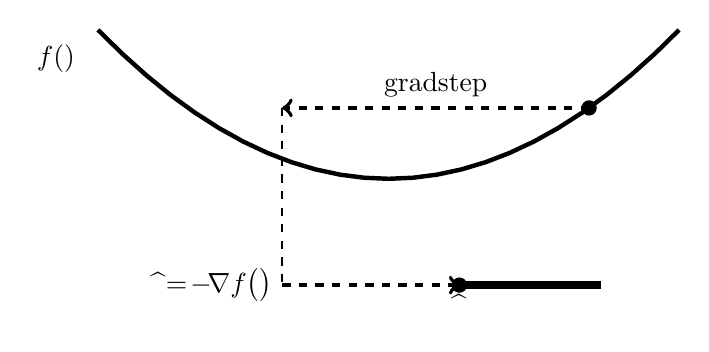
\begin{tikzpicture}[scale=0.9]
			\node [right] at (-5.1,1.7) {$f(\weights)$} ;
			\draw[ultra thick, domain=-4.1:4.1] plot (\x,  {(1/8)*\x*\x});
		%	\draw[dashed, thick, domain=1:3.6] plot (\x,  {\x - 1}) node[right] {$ f\big(\weights^{(\itercntr)}\big)\!+\!\big(\weights\!-\!\weights^{(\itercntr)}\big)^{T} \nabla f\big(\weights^{(\itercntr)}\big)$};
			\draw [fill] (2.83,1) circle [radius=0.1] node[right] {$\weights$};
			\draw[line width =0.5mm,dashed,->] (2.83,1) -- node[midway,above] {\gls{gradstep}} (-1.5,1);
			\draw[line width =0.2mm,dashed] (-1.5,1) --(-1.5,-1.5)  node [below, left]{$\widehat{\weights}=\weights\!-\!\lrate \nabla f\big(\weights\big)$} ;
			\draw[line width =0.5mm,dashed,->] (-1.5,-1.5)  -- node[midway,above] {} (1,-1.5) ; 
			\draw [fill] (1,-1.5) circle [radius=0.1] node[below] {$\projection{\paramspace}{\widehat{\weights}}$};
			\draw[line width=1mm] (1,-1.5) -- (3,-1.5) node[midway, above] {$\paramspace$};
		\end{tikzpicture}
		\vspace*{-5mm}
		\end{center}
		\caption{Projected \gls{gd} augments a basic \gls{gradstep} with a \gls{projection} back onto the constraint set $\paramspace$.}
		\label{fig_projected_GD_dict}
		\end{figure}
		\foreignlanguage{greek}{Βλέπε επίσης:} \gls{erm}, \gls{model}, \gls{paramspace}, \gls{objfunc}, \gls{smooth}, \gls{gd}, \gls{modelparams}, 
		\gls{gradstep}, \gls{projection}.},
	first={\foreignlanguage{greek}{προβεβλημένη κάθοδος κλίσης}},
	text={\foreignlanguage{greek}{προβεβλημένη κάθοδος κλίσης}},
	user1={\foreignlanguage{greek}{προβεβλημένη κάθοδος κλίσης}}, %nominative
	user2={\foreignlanguage{greek}{προβεβλημένης καθόδου κλίσης}} %genitive 
}

\newglossaryentry{predictor}
{name={\foreignlanguage{greek}{προβλέπουσα}},
	description={\foreignlanguage{greek}{Μία προβλέπουσα είναι μία} \gls{map}\index{\foreignlanguage{greek}{προβλέπουσα}} \glsentryuserii{hypothesis} 
		\foreignlanguage{greek}{πραγματικής τιμής. Δεδομένου ενός} \glsentryuserii{datapoint} \foreignlanguage{greek}{με} \glsentryuservi{feature} 
		$\featurevec$, \foreignlanguage{greek}{η τιμή $\hypothesis(\featurevec) \in \mathbb{R}$ χρησιμοποιείται ως η} \glsentryuseri{prediction} 
		\foreignlanguage{greek}{για την αληθή αριθμητική} \glsentryuseriii{label} $\truelabel \in \mathbb{R}$ \foreignlanguage{greek}{του} \glsentryuserii{datapoint}.\\
		\foreignlanguage{greek}{Βλέπε επίσης:} \gls{hypothesis}, \gls{map}, \gls{datapoint}, \gls{feature}, \gls{prediction}, \gls{label}.},
	first={\foreignlanguage{greek}{προβλέπουσα}},
	text={\foreignlanguage{greek}{προβλέπουσα}},
	user1={\foreignlanguage{greek}{προβλέπουσα}}, %nominative
  	user2={\foreignlanguage{greek}{προβλέπουσας}} %genitive 
}

\newglossaryentry{prediction}
{name={\foreignlanguage{greek}{πρόβλεψη}},
	description={\foreignlanguage{greek}{Μία πρόβλεψη}\index{\foreignlanguage{greek}{πρόβλεψη}} 
		\foreignlanguage{greek}{είναι μία εκτίμηση ή προσέγγιση για κάποια ποσότητα ενδιαφέροντος. Η} 
		\glsentryuseri{ml} \foreignlanguage{greek}{περιστρέφεται γύρω από τη μάθηση ή εύρεση μίας} \gls{map} \glsentryuserii{hypothesis} $\hypothesis$ 
		\foreignlanguage{greek}{που διαβάζει τα} \glsentryuservi{feature} $\featurevec$ \foreignlanguage{greek}{ενός} \glsentryuserii{datapoint} 
		\foreignlanguage{greek}{και δίνει μία πρόβλεψη $\widehat{\truelabel} \defeq \hypothesis(\featurevec)$ για την} \glsentryuseriii{label} 
		\foreignlanguage{greek}{του} $\truelabel$.\\
		\foreignlanguage{greek}{Βλέπε επίσης:} \gls{ml}, \gls{hypothesis}, \gls{map}, \gls{feature}, \gls{datapoint}, \gls{label}.},
	first={\foreignlanguage{greek}{πρόβλεψη}},
	text={\foreignlanguage{greek}{πρό\-βλε\-ψη}},
	user1={\foreignlanguage{greek}{πρόβλεψη}}, %nominative
  	user2={\foreignlanguage{greek}{πρόβλεψης}}, %genitive 
	user3={\foreignlanguage{greek}{πρόβλεψη}}, %accusative
	user4={\foreignlanguage{greek}{προβλέψεις}}, %nominativepl  
	user5={\foreignlanguage{greek}{προβλέψεων}}, %genitivepl
	user6={\foreignlanguage{greek}{προβλέψεις}}, %accusativepl
	user7={\foreignlanguage{greek}{προβλέψεών}}, %genitivepldoublestress
	user8={\foreignlanguage{greek}{πρόβλεψής}} %genitivedoublestress 
}

\newglossaryentry{optproblem}
{name={\foreignlanguage{greek}{πρόβλημα βελτιστοποίησης}}, 
	description={\foreignlanguage{greek}{Ένα πρόβλημα βελτιστοποίησης}\index{\foreignlanguage{greek}{πρόβλημα βελτιστοποίησης}} 
		(optimization problem) \foreignlanguage{greek}{είναι μία μαθηματική δομή που αποτελείται από μία} \glsentryuseriii{objfunc} 
		$f: \mathcal{U} \rightarrow \mathcal{V}$ \foreignlanguage{greek}{ορισμένη πάνω σε μία μεταβλητή βελτιστοποίησης 
		$\weights \in \mathcal{U}$, μαζί με ένα εφικτό σύνολο $\mathcal{W} \subseteq \mathcal{U}$. Το 
		πεδίο τιμών $\mathcal{V}$ θεωρείται ότι είναι διατεταγμένο, που σημαίνει ότι για οποιαδήποτε δύο στοιχεία 
		$\mathbf{a}, \mathbf{b} \in \mathcal{V}$, μπορούμε να καθορίσουμε αν $\mathbf{a} < \mathbf{b}$, $\mathbf{a} = \mathbf{b}$, 
		ή $\mathbf{a} > \mathbf{b}$. Ο στόχος της βελτιστοποίησης είναι να βρούμε εκείνες τις τιμές $\weights \in \mathcal{W}$ 
		για τις οποίες η αντικειμενική $f(\weights)$ είναι ακρότατη—δηλαδή ελάχιστη ή μέγιστη} 
		\cite{BertsekasNonLinProgr}, \cite{BoydConvexBook}, \cite{nesterov04}.\\
		\foreignlanguage{greek}{Βλέπε επίσης:} \gls{objfunc}.},
	first={\foreignlanguage{greek}{πρόβλημα βελτιστοποίησης}},
	text={optimization problem},
	user1={\foreignlanguage{greek}{πρόβλημα βελτιστοποίησης}}, %nominative
  	user2={\foreignlanguage{greek}{προβλήματος βελτιστο\-ποί\-ησης}}, %genitive 
	user3={\foreignlanguage{greek}{πρόβλημα βελτιστοποίησης}} %accusative
}

 \newglossaryentry{projection}
 {name={\foreignlanguage{greek}{προβολή}}, 
       description={\foreignlanguage{greek}{Θεωρούμε ένα υποσύνολο}\index{\foreignlanguage{greek}{προβολή}} $\paramspace \subseteq \mathbb{R}^{\dimlocalmodel}$ 
       		\foreignlanguage{greek}{του $\dimlocalmodel$-διάστατου} \glsentryuserii{euclidspace}. \foreignlanguage{greek}{Ορίζουμε την προβολή 
		$\projection{\paramspace}{\weights}$ ενός διανύσματος $\weights \in \mathbb{R}^{\dimlocalmodel}$ στο $\paramspace$ ως}
		\begin{equation} 
   	    		\label{equ_def_proj_generic_dict}
  	     		\projection{\paramspace}{\weights} = \aargmin_{\weights' \in \paramspace} \normgeneric{\weights - \weights'}{2}. 
         	\end{equation}
		 \foreignlanguage{greek}{Με άλλα λόγια, η $\projection{\paramspace}{\weights}$ είναι το διάνυσμα στο $\paramspace$ που είναι 
		 πιο κοντά στο $\weights$. Η προβολή είναι καλά ορισμένη μόνο για υποσύνολα $\paramspace$ για τα οποία 
		 υπάρχει το παραπάνω} \glsentryuseri{minimum} \cite{BoydConvexBook}.\\
		 \foreignlanguage{greek}{Βλέπε επίσης:} \gls{euclidspace}, \gls{minimum}.},
	first={\foreignlanguage{greek}{προβολή}},
	text={\foreignlanguage{greek}{προβολή}},
	user1={\foreignlanguage{greek}{προβολή}}, %nominative
	user2={\foreignlanguage{greek}{προβολής}} %genitive 
}

\newglossaryentry{expectation}
{name={\foreignlanguage{greek}{προσδοκία}}, 
 	description={\foreignlanguage{greek}{Θεωρούμε ένα αριθμητικό}\index{expectation} \glsentryuseriii{featurevec} $\featurevec \in \mathbb{R}^{\featuredim}$ 
		\foreignlanguage{greek}{το οποίο ερμηνεύουμε ως την} \glsentryuseriii{realization} \foreignlanguage{greek}{μίας} \glsentryuserii{rv} 
		\foreignlanguage{greek}{με μία} \glsentryuseriii{probdist} $p(\featurevec)$. 
		\foreignlanguage{greek}{Η προσδοκία του $\featurevec$ ορίζεται ως το ολοκλήρωμα $\expect \{ \featurevec \} \defeq \int \featurevec p(\featurevec)$. 
		Σημείωση ότι η προσδοκία ορίζεται μόνο αν υφίσταται αυτό το ολοκλήρωμα, δηλαδή αν η} \glsentryuseri{rv} \foreignlanguage{greek}{είναι 
		ολοκληρώσιμη} \cite{RudinBookPrinciplesMatheAnalysis}, \cite{BillingsleyProbMeasure}, \cite{HalmosMeasure}. 
		\foreignlanguage{greek}{Το Σχ.} \ref{fig_expect_discrete_dict} \foreignlanguage{greek}{απεικονίζει την προσδοκία μίας βαθμωτής διακριτής} 
		\glsentryuserii{rv} $x$ \foreignlanguage{greek}{που παίρνει τιμές μόνο από ένα πεπερασμένο σύνολο.} 
   		\begin{figure}[H]
   			\begin{center}
   			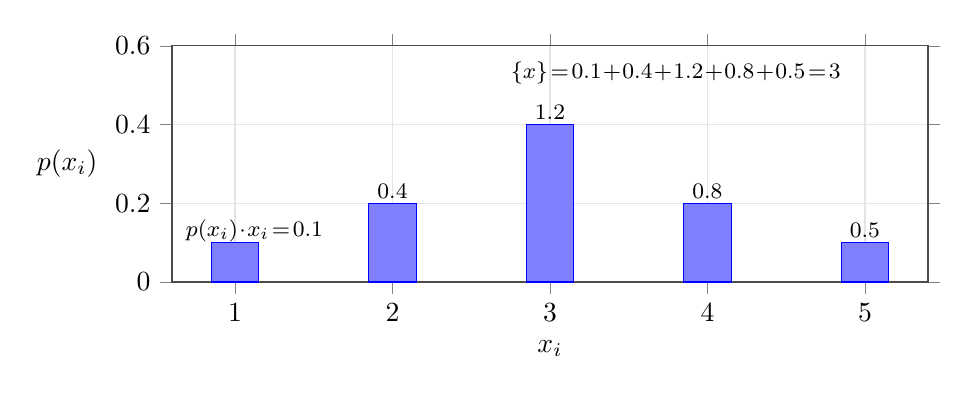
\begin{tikzpicture}
			\begin{axis}[
			ybar,
			y=5cm,
			x=2cm,                          % ⬅️ Controls spacing between bars
			bar width=0.6cm,                   % ⬅️ Controls bar thickness
		%	bar shift=-0.5cm,                % ⬅️ Center bars (=-0.5 * bar width)
			xlabel={$x_i$},
			clip=false,
			ylabel={$p(x_i)$},
			y label style={rotate=-90, anchor=west, xshift=-1cm},
			xtick={1,2,3,4,5},
			ymin=0, ymax=0.6,
			grid=both,
			major grid style={gray!20},
			tick align=outside,
			axis line style={black!70},
			]
			\addplot+[ybar, fill=blue!50] coordinates {
				(1,0.1) 
				(2,0.2) 
				(3,0.4) 
				(4,0.2)
				(5,0.1)
			};
			% Manual textboxes above bars
			\node[font=\footnotesize,xshift=7pt] at (axis cs:1,0.13) {$p(x_i)\!\cdot\!x_i\!=\!0.1$};
			\node[font=\footnotesize]at (axis cs:2,0.23) {$0.4$};
			\node[font=\footnotesize]at (axis cs:3,0.43) {$1.2$};
			\node[font=\footnotesize] at (axis cs:4,0.23) {$0.8$};
			\node[font=\footnotesize]at (axis cs:5,0.13) {$0.5$};
			\node[font=\footnotesize]at (axis cs:3.8,0.53) {$\expect\{x\}\!=\!0.1\!+\!0.4\!+\!1.2\!+\!0.8\!+\!0.5\!=\!3$};
			\end{axis}
			\end{tikzpicture}
			\end{center}
			\vspace*{-5mm}
			{\selectlanguage{greek}
			\caption{\foreignlanguage{greek}{Η προσδοκία μίας διακριτής} \glsentryuserii{rv} $x$ \foreignlanguage{greek}{προκαλείται από το 
			άρθροισμα των πιθανών τιμών της $x_{i}$, σταθμισμένες από την αντίστοιχη} \glsentryuseriii{probability} $p(x_i) = \prob{x= x_i}$. 
			\label{fig_expect_discrete_dict}} }
 		\end{figure}
		\foreignlanguage{greek}{Βλέπε επίσης:} \gls{featurevec}, \gls{realization}, \gls{rv}, \gls{probdist}, \gls{probability}.},
 	first={\foreignlanguage{greek}{προσδοκία}},
 	text={expectation},
	user1={\foreignlanguage{greek}{προσδοκία}}, %nominative
 	user2={\foreignlanguage{greek}{προσδοκίας}}, %genitive   
 	user3={\foreignlanguage{greek}{προσδοκία}}, %accusative
	user4={\foreignlanguage{greek}{προσδοκίες}}, %nominative
 	user5={\foreignlanguage{greek}{προσδοκιών}}, %genitive   
 	user6={\foreignlanguage{greek}{προσδοκίες}} %accusative
}

\newglossaryentry{proximable}
{name={\foreignlanguage{greek}{προσεγγίσιμος}},
	description={\foreignlanguage{greek}{Μία}\index{\foreignlanguage{greek}{προσεγγίσιμος}} 
		\glsentryuseriii{convex} \glsentryuseri{function} \foreignlanguage{greek}{για την οποία ο} \glsentryuseri{proxop} 
		\foreignlanguage{greek}{μπορεί να υπολογιστεί αποτελεσματικά αναφέρεται μερικές φορές ως 
		προσεγγίσιμη ή απλή} \cite{Condat2013}.\\
		\foreignlanguage{greek}{Βλέπε επίσης:} \gls{convex}, \gls{function}, \gls{proxop}.},
	first={\foreignlanguage{greek}{προσεγγίσιμος}},
	text={\foreignlanguage{greek}{προσεγγίσιμος}},
	user1={\foreignlanguage{greek}{προσεγγίσιμος}}, %nominative
	user2={\foreignlanguage{greek}{προσεγγίσιμου}} %genitive 
}

\newglossaryentry{privprot}
{name={\foreignlanguage{greek}{προστασία της ιδιωτικότητας}},
     description={\foreignlanguage{greek}{Θεωρούμε κάποια μέθοδο}\index{\foreignlanguage{greek}{προστασία της ιδιωτικότητας}} \glsentryuserii{ml} $\algomap$ 
        		\foreignlanguage{greek}{που διαβάζει ένα} 
		\glsentryuseriii{dataset} $\dataset$ \foreignlanguage{greek}{και δίνει κάποια έξοδο $\algomap(\dataset)$. Η έξοδος 
		θα μπορούσε να είναι οι} \glsentryuseri{modelparams} $\widehat{\weights}$ \foreignlanguage{greek}{που μαθαί\-νονται ή η} \glsentryuseri{prediction} 
		$\learnthypothesis(\featurevec)$ \foreignlanguage{greek}{που προκύπτει για ένα συγκεκριμένο} \glsentryuseriii{datapoint} \foreignlanguage{greek}{με} 
		\glsentryuservi{feature} $\featurevec$. \foreignlanguage{greek}{Πολλές σημαντικές εφαρμογές} \glsentryuserii{ml} 
		\foreignlanguage{greek}{περιλαμβάνουν} \glsentryuservi{datapoint} \foreignlanguage{greek}{που αντιπροσωπεύουν ανθρώπους. Κάθε} 
		\glsentryuseri{datapoint} \foreignlanguage{greek}{χαρακτηρίζεται από} \glsentryuservi{feature} $\featurevec$, 
		\foreignlanguage{greek}{ενδεχομένως μία} \glsentryuseriii{label} $\truelabel$, \foreignlanguage{greek}{και ένα} \glsentryuseriii{sensattr} $\sensattr$ 
		\foreignlanguage{greek}{(π.χ. μία πρόσφατη ιατρική διάγνωση). 
		Στο περίπου, προστασία της ιδιωτικότητας σημαίνει ότι θα έπρεπε να είναι αδύνατο να συμπεράνουμε, από την έξοδο $\algomap(\dataset)$, 
		οποιοδήποτε από τα} \glsentryuservi{sensattr} \foreignlanguage{greek}{των} \glsentryuserv{datapoint} \foreignlanguage{greek}{στο} $\dataset$. 
		\foreignlanguage{greek}{Από μαθηματικής άποψης, η προστασία της ιδιωτικότητας απαιτεί την μη αντιστρεψιμότητα της} \gls{map}  
		$\algomap(\dataset)$. \foreignlanguage{greek}{Γενικά, το να κάνουμε απλώς το $\algomap(\dataset)$ μη αντιστρέψιμο 
		είναι συνήθως ανεπαρκές για την προστασία της ιδιωτικότητας. Χρειάζεται να κάνουμε το $\algomap(\dataset)$ επαρκώς μη αντιστρέψιμο.}\\
		\foreignlanguage{greek}{Βλέπε επίσης:} \gls{ml}, \gls{dataset}, \gls{modelparams}, \gls{prediction}, \gls{datapoint}, \gls{feature}, \gls{label}, \gls{sensattr}, \gls{map}.}, 
	first={\foreignlanguage{greek}{προστασία της ιδιωτικότητας}}, 
	text={\foreignlanguage{greek}{προστασία της ιδιωτικότητας}},
	user1={\foreignlanguage{greek}{προστασία της ιδιωτικότητας}}, %nominative
   	user2={\foreignlanguage{greek}{προστασίας της ιδιωτικότητας}} %genitive   
}

\newglossaryentry{kernel}
{name={\foreignlanguage{greek}{πυρήνας}}, 
	description={Consider\index{\foreignlanguage{greek}{πυρήνας}} a set of \gls{datapoint}s, each represented by a \gls{featurevec} 
%	 	$\featurevec \in \featurespace$, where $\featurespace$ denotes the \gls{featurespace}. 
%	 	A (real-valued) kernel is a \gls{function} 
%	 	$\kernel: \featurespace \times \featurespace \rightarrow \mathbb{R}$ that assigns to every pair of 
%     		\gls{featurevec}s $\featurevec, \featurevec' \in \featurespace$ a real number $\kernelmap{\featurevec}{\featurevec'}$. 
%     		This value is typically interpreted as a similarity measure between $\featurevec$ and $\featurevec'$. 
%	 	The defining property of a kernel is that it is symmetric, i.e.,
%	 	$\kernelmap{\featurevec}{\featurevec'} = \kernelmap{\featurevec'}{\featurevec}$, and that 
%	 	for any finite set of \gls{featurevec}s $\featurevec_1, \ldots, \featurevec_n \in \featurespace$, the matrix 
%	  	\begin{equation}
%	 		\nonumber
%	 		\mathbf{K} = \begin{pmatrix}
%	 			\kernelmap{\featurevec_1}{\featurevec_1} & \kernelmap{\featurevec_1}{\featurevec_2} & \ldots & \kernelmap{\featurevec_1}{\featurevec_n} \\
%	 			\kernelmap{\featurevec_2}{\featurevec_1} & \kernelmap{\featurevec_2}{\featurevec_2} & \ldots & \kernelmap{\featurevec_2}{\featurevec_n} \\
%	 			\vdots											
%	 			& \vdots & \ddots & \vdots \\
%	 			\kernelmap{\featurevec_n}{\featurevec_1} & \kernelmap{\featurevec_n}{\featurevec_2} & \ldots & \kernelmap{\featurevec_n}{\featurevec_n} 
%	 		\end{pmatrix} \in \mathbb{R}^{n \times n}
%	 	\end{equation}
%	 	is \gls{psd}. 
%     		A kernel naturally defines a transformation of a \gls{featurevec} $\featurevec$ into a 
%	 	\gls{function} $\vz = \kernelmap{\featurevec}{\cdot}$. The \gls{function} $\vz$ maps an  
%	 	input $\featurevec' \in \featurespace$ to the value $\kernelmap{\featurevec}{\featurevec'}$. 
%	 	We can view the \gls{function} $\vz$ as a new \gls{featurevec} that belongs to a 
%	 	\gls{featurespace} $\featurespace'$ which is typically different from $\featurespace$. 
%	 	This new \gls{featurespace} $\featurespace'$ has a particular mathematical structure, i.e., it is a 
%	 	reproducing kernel \gls{hilbertspace} (RKHS)~\cite{LearningKernelsBook}, \cite{LampertNowKernel}.
%     		Since $\vz$ belongs to a RKHS, which is a \gls{vectorspace}, we can interpret it as a generalized 
%	 	\gls{featurevec}. Note that a finite-length \gls{featurevec} $\featurevec=\big(\feature_{1},\ldots,\feature_{\nrfeatures} \big)\,^{T} \in \mathbb{R}^{\nrfeatures}$ 
%	 	can be viewed as a \gls{function} $\featurevec: \{1, \ldots, \nrfeatures\} \rightarrow \mathbb{R}$ 
%	 	that assigns a real value to each index $\featureidx \in \{1,\ldots,\nrfeatures\}$. 
%			\\
%          	\foreignlanguage{greek}{Βλέπε επίσης:} \gls{datapoint}, \gls{featurevec}, \gls{featurespace}, \gls{function}, \gls{psd}, 
%		\gls{hilbertspace}, \gls{vectorspace}, \gls{kernelmethod}. 
		},
	first={\foreignlanguage{greek}{πυρήνας}},
	text={\foreignlanguage{greek}{πυρήνας}},
	user1={\foreignlanguage{greek}{πυρήνας}}, %nominative
  	user2={\foreignlanguage{greek}{πυρήνα}}, %genitive  
	user3={\foreignlanguage{greek}{πυρήνα}} %accusative
}

\newglossaryentry{learnrate}
{name={\foreignlanguage{greek}{ρυθμός μάθησης}}, 
	description={\foreignlanguage{greek}{Θεωρούμε μία επαναληπτική μέθοδο}\index{\foreignlanguage{greek}{ρυθμός μάθησης}} 
		\glsentryuserii{ml} \foreignlanguage{greek}{για την εύρεση ή μάθηση μίας χρήσιμης} \glsentryuserii{hypothesis} $\hypothesis \in \hypospace$. 
		\foreignlanguage{greek}{Μία τέτοια επαναληπτική μέθοδος επαναλαμβάνει όμοια υπολογιστικά βήματα (ενημέρωσης) που  
		προσαρμόζουν ή τροποποιούν την τρέχουσα} \glsentryuseriii{hypothesis} \foreignlanguage{greek}{για να προκύψει μία βελτιωμένη} 
		\glsentryuseriii{hypothesis}. \foreignlanguage{greek}{Ένα καλά γνωστό παράδειγμα μίας τέτοιας επαναληπτικής μεθόδου μάθησης είναι η}  
		\glsentryuseri{gd} \foreignlanguage{greek}{και οι παραλλαγές της,} \glsentryuseri{stochGD} \foreignlanguage{greek}{και}  
		\glsentryuseri{projgd}. \foreignlanguage{greek}{Μία} \glsentryuseri{parameter}-\foreignlanguage{greek}{κλειδί μίας επαναληπτικής μεθόδου 
		είναι ο ρυθμός μάθησης. Ο ρυθμός μάθησης ελέγχει τον βαθμό που η τρέχουσα} \glsentryuseri{hypothesis} \foreignlanguage{greek}{μπορεί να 
		τροποποιηθεί κατά τη διάρκεια μίας μονής επανάληψης. Ένα καλά γνωστό παράδειγμα μίας τέτοιας} \glsentryuserii{parameter} \foreignlanguage{greek}{είναι 
		το} \glsentryuseri{stepsize} \foreignlanguage{greek}{που χρησιμοποιείται στην} \glsentryuseriii{gd} \cite[\foreignlanguage{greek}{Κεφ.} 5]{MLBasics}.\\
		\foreignlanguage{greek}{Βλέπε επίσης:} \gls{ml}, \gls{hypothesis}, \gls{gd}, \gls{stochGD}, \gls{projgd}, \gls{parameter}, \gls{stepsize}.},
	first={\foreignlanguage{greek}{ρυθμός μάθησης}},
	text={\foreignlanguage{greek}{ρυθμός μάθησης}},
	user1={\foreignlanguage{greek}{ρυθμός μάθησης}}, %nominative
  	user2={\foreignlanguage{greek}{ρυθμού μάθησης}}, %genitive  
	user3={\foreignlanguage{greek}{ρυθμό μάθησης}} %accusative
}

\newglossaryentry{datapoint}
{name={\foreignlanguage{greek}{σημείο δεδομένων}},
	description={\foreignlanguage{greek}{Ένα σημείο}\index{\foreignlanguage{greek}{σημείο δεδομένων}} \glsentryuserii{data} 
		\foreignlanguage{greek}{είναι οποιοδήποτε αντικείμενο που μεταφέρει πληροφορίες} \cite{coverthomas}. 
		\foreignlanguage{greek}{Παραδείγματα περιλαμβάνουν μαθητές, ραδιοσήματα, δέντρα, εικόνες,} \glsentryuservi{rv}, 
		\foreignlanguage{greek}{πραγματικούς αριθ\-μούς, ή πρωτεΐνες. Περιγράφουμε σημεία} \glsentryuserii{data} 
		\foreignlanguage{greek}{του ίδιου τύπου με δύο κατηγορίες ιδιοτήτων:} 
%		\begin{enumerate}[label=\arabic*)]
%   			\item \foreignlanguage{greek}{Τα} \glsentryuseriv{feature} \foreignlanguage{greek}{είναι μετρήσιμες ή 
%			υπολογίσιμες ιδιότητες ενός σημείου} \glsentryuserii{data}. \foreignlanguage{greek}{Αυτά τα 
%    			ιδιοχαρακτηριστικά μπορούν να εξαχθούν ή να υπολογιστούν αυτόματα χρησιμοποιώντας αισθητήρες, 
%			υπολογιστές, ή άλλα συστήματα συλλογής} \glsentryuserii{data}. \foreignlanguage{greek}{Για ένα σημείο}  
%			\glsentryuserii{data} \foreignlanguage{greek}{που αναπαριστά έναν ασθενή, ένα} \glsentryuseri{feature} 
%			\foreignlanguage{greek}{θα μπορούσε να είναι το σωματικό βάρος.} 
%    			\item \foreignlanguage{greek}{Οι} \glsentryuseriv{label} \foreignlanguage{greek}{είναι γεγονότα υψηλότερου
%			επιπέδου (ή ποσότητες ενδιαφέροντος) που σχετίζονται με το σημείο} \glsentryuserii{data}.
%			\foreignlanguage{greek}{Ο προσδιορισμός των} \glsentryuserv{label} \foreignlanguage{greek}{ενός σημείου} 
%			\glsentryuserii{data} \foreignlanguage{greek}{συνήθως απαιτεί ανθρώπινη εμπειρογνωσία ή γνώση πεδίου. 
%			Για ένα σημείο} \glsentryuserii{data} \foreignlanguage{greek}{που αναπαριστά έναν ασθενή,
%			μία διάγνωση καρκίνου που έχει παραχθεί από έναν γιατρό θα μπορούσε να χρησιμεύει ως η} \glsentryuseri{label}.
%		\end{enumerate}
%		Fig.\ \ref{fig:datapoint_cowherd_dict} depicts an image as an example of a \gls{data} 
%		point along with its \gls{feature}s and \gls{label}s. Importantly, what constitutes 
%		a \gls{feature} or a \gls{label} is not inherent to the \gls{data} point itself—it is a design 
%		choice that depends on the specific \gls{ml} applicaton.
%		\begin{figure}[H]
%    		\centering
%    			% Image as a datapoint
%    			\begin{minipage}[t]{0.95\textwidth}
%        		\centering
%        		\includegraphics[width=\textwidth]{assets/CowsAustria.jpg}
%        		\caption*{A single \gls{data} point.}
%        		\vspace{5mm}
%    			\end{minipage}
%    			% Feature and label description
%    			\begin{minipage}[t]{0.95\textwidth}
%        		\Gls{feature}s:
%        		\begin{itemize}
%            			\item $x_{1},\ldots,x_{\nrfeatures_{1}}$: Colour intensities of all image pixels.
%           			\item $x_{\nrfeatures_{1}+1}$: Time-stamp of the image capture.
%            			\item $x_{\nrfeatures_{1}+2}$: Spatial location of the image capture.
%			\end{itemize}
%			\Gls{label}s:
%            		\begin{itemize}
%               	 	\item $\truelabel_{1}$: Number of cows depicted. 
%                		\item $\truelabel_{2}$: Number of wolves depicted. 
%                		\item $\truelabel_{3}$: Condition of the pasture (e.g., healthy, overgrazed).
%            		\end{itemize}
%    			\end{minipage}
%    			\caption{Illustration of a \gls{data} point consisting of an image. We can use 
%			different properties of the image as \gls{feature}s and higher-level facts
%			about the image as \gls{label}s.\label{fig:datapoint_cowherd_dict}}
%		\end{figure}
%		\foreignlanguage{greek}{Η διάκριση μεταξύ} \glsentryuserv{feature} \foreignlanguage{greek}{και} \glsentryuserv{label} 
%		\foreignlanguage{greek}{δεν είναι πάντα ξεκάθαρη. Μία ιδιότητα που θεωρείται μία} \glsentryuseri{label}
% 		\foreignlanguage{greek}{σε ένα περιβάλλον (π.χ. μία διάγνωση καρκίνου) μπορεί να αντιμετωπίζεται ως ένα} 
% 		\glsentryuseri{feature} \foreignlanguage{greek}{σε ένα άλλο περιβάλλον—ιδιαίτερα αν η αξιόπιστη αυτοματοποίηση  
% 		(π.χ. μέσω ανάλυσης εικόνων) επιτρέπει τον υπολογισμό της χωρίς ανθρώπινη παρέμβαση. Η} \glsentryuseri{ml} 
%   		\foreignlanguage{greek}{στοχεύει γενικά στην πρόβλεψη της} \glsentryuserii{label} \foreignlanguage{greek}{ενός σημείου} 
%		\glsentryuserii{data} \foreignlanguage{greek}{με βάση μόνο τα} \glsentryuservi{feature} \foreignlanguage{greek}{του}. 
		\\
		\foreignlanguage{greek}{Βλέπε επίσης:} \gls{data}, \gls{rv}, \gls{feature}, \gls{label}, \gls{ml}, \gls{dataset}.}, 
	first={data point},
	text={data point},
	user1={\foreignlanguage{greek}{σημείο δεδομένων}}, %nominative
	user2={\foreignlanguage{greek}{σημείου δεδομένων}}, %genitive
	user3={\foreignlanguage{greek}{σημείο δεδομένων}}, %accusative
	user4={\foreignlanguage{greek}{σημεία δεδομένων}}, %nominativepl
	user5={\foreignlanguage{greek}{σημείων δεδομένων}}, %genitivepl
	user6={\foreignlanguage{greek}{ση\-μεί\-α δεδομένων}} %accusativepl        
}

\newglossaryentry{labeled datapoint}
{name={\foreignlanguage{greek}{σημείο δεδομένων με ετικέτα}},
 	description={\foreignlanguage{greek}{Ένα}\index{\foreignlanguage{greek}{σημείο δεδομένων με ετικέτα}} \glsentryuseri{datapoint} 
		\foreignlanguage{greek}{του οποίου η} \glsentryuseri{label} \foreignlanguage{greek}{είναι γνωστή ή έχει προσδιοριστεί με κάποιον 
		τρόπο που μπορεί να απαιτεί ανθρώπινη εργασία.} \\
		\foreignlanguage{greek}{Βλέπε επίσης:} \gls{datapoint}, \gls{label}.},
 	first={\foreignlanguage{greek}{σημείο δεδομένων με ετικέτα}},
 	text={\foreignlanguage{greek}{σημείο δεδομένων με ετικέτα}},
 	user1={\foreignlanguage{greek}{σημείο δεδομένων με ετικέτα}}, %nominative
 	user2={\foreignlanguage{greek}{σημείου δεδομένων με ετικέτα}}, %genitive  
 	user3={\foreignlanguage{greek}{σημείο δεδομένων με ετικέτα}}, %accusative
 	user4={\foreignlanguage{greek}{σημεία δεδομένων με ετικέτες}}, %nominativepl  
 	user5={\foreignlanguage{greek}{σημείων δεδομένων με ετικέτες}}, %genitivepl
 	user6={\foreignlanguage{greek}{σημεία δεδομένων με ετικέτες}} %accusativepl  
}

\newglossaryentry{hardclustering}
{name={\foreignlanguage{greek}{σκληρή συσταδοποίηση}}, 
	description={\foreignlanguage{greek}{Η σκληρή} 
		\glsentryuseri{clustering}\index{\foreignlanguage{greek}{σκληρή συσταδοποίηση}} 
		\foreignlanguage{greek}{αναφέρεται στην εργασία χωρισμού ενός συγκεκριμένου συνόλου} \glsentryuserv{datapoint} 
		\foreignlanguage{greek}{σε (μερικές) μη αλληλεπικαλυπτόμενες} \glsentryuservi{cluster}. 
		\foreignlanguage{greek}{Η πιο ευρέως χρησιμοποιούμενη μέθοδος σκληρής} \glsentryuserii{clustering} \foreignlanguage{greek}{είναι ο} 
		\glsentryuseri{kmeans}.\\
		\foreignlanguage{greek}{Βλέπε επίσης:} \gls{clustering}, \gls{datapoint}, \gls{cluster}, \gls{kmeans}.},
	first={hard clustering},
	text={hard clustering},
	user1={\foreignlanguage{greek}{σκληρή συσταδοποίηση}}, %nominative
	user2={\foreignlanguage{greek}{σκληρής συσταδοποίησης}} %genitive   
}

\newglossaryentry{statasp}
{name={\foreignlanguage{greek}{στατιστικές διαστάσεις}}, 
	description={\foreignlanguage{greek}{Ως στατιστικές διαστάσεις μίας μεθόδου}\index{\foreignlanguage{greek}{στατιστικές διαστάσεις}} 
		\glsentryuserii{ml}, \foreignlanguage{greek}{αναφερόμαστε σε (ιδιότητες της)} \glsentryuseriii{probdist} \foreignlanguage{greek}{της 
		εξόδου της κάτω από ένα} \glsentryuseriii{probmodel} \foreignlanguage{greek}{για τα} \glsentryuseriii{data} 
		\foreignlanguage{greek}{που τροφοδοτούνται στη μέθοδο.} \\
		\foreignlanguage{greek}{Βλέπε επίσης:} \gls{ml}, \gls{probdist}, \gls{probmodel}, \gls{data}.},
	first={\foreignlanguage{greek}{στατιστικές διαστάσεις}},
	text={\foreignlanguage{greek}{στατιστικές διαστάσεις}},
	user1={\foreignlanguage{greek}{στατιστικές διαστάσεις}}, %nominativepl
	user2={\foreignlanguage{greek}{στατιστικών διαστάσεων}}, %genitivepl 
	user3={\foreignlanguage{greek}{στατιστικές διαστάσεις}} %accusativepl 
}

\newglossaryentry{stochastic}
{name={\foreignlanguage{greek}{στοχαστική}},
	description={\foreignlanguage{greek}{Αναφερόμαστε σε μία μέθοδο ως στοχαστιή}\index{stochastic} 
		\foreignlanguage{greek}{αν περιλαμβάνει μία τυχαία συνιστώσα ή διέπεται από πιθανοτικούς 
		νόμους. Οι μέθοδοι} \glsentryuserii{ml} \foreignlanguage{greek}{χρησιμοποιούν τυχαιότητα για να 
		μειώσουν την υπολογιστική πολυπλοκότητα (π.χ. βλέπε} \glsentryuseri{stochGD}) 
		\foreignlanguage{greek}{ή για να αποτυπώσουν την} \glsentryuseriii{uncertainty} 
		\foreignlanguage{greek}{σε} \glsentryuservi{probmodel}. \\
		\foreignlanguage{greek}{Βλέπε επίσης:} \gls{ml}, \gls{stochGD}, \gls{uncertainty}, \gls{probmodel}.},
	first={\foreignlanguage{greek}{στοχαστική}},
	text={\foreignlanguage{greek}{στοχαστική}}, 
	user1={\foreignlanguage{greek}{στοχαστική}}, %nominative
	user2={\foreignlanguage{greek}{στοχαστικής}}, %genitive
	user3={\foreignlanguage{greek}{στοχαστική}}, %accusative
	user4={\foreignlanguage{greek}{στοχαστικός}}, %nominativemasc
	user5={\foreignlanguage{greek}{στοχαστικού}}, %genitivemasc
	user6={\foreignlanguage{greek}{στοχαστικό}}, %accusativemasc
	user7={\foreignlanguage{greek}{στοχαστικές}}, %nominativeoraccusativeplfem
	user8={\foreignlanguage{greek}{στοχαστικών}} %genitiveplfemormasc
}

\newglossaryentry{stochproc}
{name={\foreignlanguage{greek}{στοχαστική διαδικασία}},
	description={\foreignlanguage{greek}{Μία} \glsentryuseri{stochastic}\index{\foreignlanguage{greek}{στοχαστική διαδικασία}} 
		\foreignlanguage{greek}{διαδικασία είναι μία συλλογή} \glsentryuserv{rv} \foreignlanguage{greek}{που ορίζονται πάνω 
		σε έναν κοινό} \glsentryuseriii{probspace}. \foreignlanguage{greek}{Αυτές οι} \glsentryuseriv{rv} \foreignlanguage{greek}{είναι 
		με δείκτες για χρόνο και χώρο και χρησιμοποιούνται για να μοντελοποιήσουν τυχαία φαινόμενα που 
		εξελίσσονται προοδευτικά (π.χ. θόρυβο σε αισθητήρες ή οικονομικές χρονοσειρές). Τυχαίοι} \glsentryuseriv{graph}, 
		\foreignlanguage{greek}{όπως το} \glsentryuseri{sbm} \foreignlanguage{greek}{ή ο} \gls{ergraph}, 
		\foreignlanguage{greek}{είναι ένα άλλο παράδειγμα} \glsentryuserviii{stochastic} \foreignlanguage{greek}{διαδικασιών. 
		Αυτές οι διαδικασίες χρησιμοποιούν ζεύγη κόμβων σε έναν} \glsentryuseriii{graph} \foreignlanguage{greek}{ως το σύνολο 
		δεικτών. Μπορούμε επίσης να χρησιμοποιήσουμε} \glsentryuservii{stochastic} \foreignlanguage{greek}{διαδικασίες 
		για να αναπαραστήσουμε} \glsentryuservi{stochalgorithm} \foreignlanguage{greek}{όπως τη} \glsentryuseriii{stochGD}. \\
		\foreignlanguage{greek}{Βλέπε επίσης:} \gls{stochastic}, \gls{rv}, \gls{probspace}, \gls{graph}, \gls{sbm}, \gls{ergraph}, 
		\gls{stochalgorithm}, \gls{stochGD}, \gls{uncertainty}, \gls{probmodel}.},
	first={\foreignlanguage{greek}{στοχαστική διαδικασία}},
	text={\foreignlanguage{greek}{στοχαστική διαδικασία}},
	user1={\foreignlanguage{greek}{στοχαστική διαδικασία}}, %nominative
  	user2={\foreignlanguage{greek}{στοχαστικής διαδικασίας}}, %genitive
	user3={\foreignlanguage{greek}{στοχαστική διαδικασία}} %accusative
}

\newglossaryentry{stochGD}
{name={\foreignlanguage{greek}{στοχαστική κάθοδος κλίσης}}, 
	description={SGD\index{\foreignlanguage{greek}{στοχαστική κάθοδος κλίσης}} 
		(stochastic gradient descent; SGD) is obtained from \gls{gd} by replacing the \gls{gradient} of the \gls{objfunc} 
		with a \gls{stochastic} approximation. A main application of SGD 
		is to train a parametrized \gls{model} via \gls{erm} on a \gls{trainset} $\dataset$ that 
		is either very large or not readily available (e.g., when \gls{datapoint}s are stored 
		in a database distributed all over the planet). To evaluate the \gls{gradient} of the 
		\gls{emprisk} (as a \gls{function} of the \gls{modelparams} $\weights$), 
		we need to compute a sum $\sum_{\sampleidx=1}^{\samplesize} \nabla_{\weights} \lossfunc{\datapoint^{(\sampleidx)}}{\weights}$  
		over all \gls{datapoint}s in the \gls{trainset}. We obtain a \gls{stochastic} 
		approximation to the \gls{gradient} by replacing the sum 
		$\sum_{\sampleidx=1}^{\samplesize} \nabla_{\weights} \lossfunc{\datapoint^{(\sampleidx)}}{\weights}$ 
		with a sum $\sum_{\sampleidx \in \batch} \nabla_{\weights} \lossfunc{\datapoint^{(\sampleidx)}}{\weights}$ 
		over a randomly chosen subset $\batch \subseteq \{1, \ldots, \samplesize\}$ (see Fig. \ref{fig_sgd_approx_dict}). 
		We often refer to these randomly chosen \gls{datapoint}s as a \gls{batch}. 
		The \gls{batch} size $|\batch|$ is an important \gls{parameter} of SGD. 
		SGD with $|\batch|> 1$ is referred to as mini-\gls{batch} SGD \cite{Bottou99}. 		
		\begin{figure}[H]
			\centering
			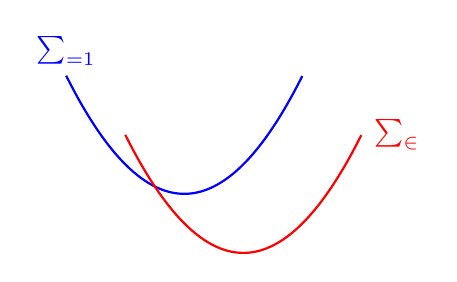
\begin{tikzpicture}[scale=1.5, >=stealth]
				\draw[thick, blue, domain=0.5:2.5, samples=100] plot (\x, {(\x-1.5)^2 + 1});
				\node[blue,above] at (0.5, 2) {$\sum_{\sampleidx=1}^{\samplesize}$};
				\draw[thick, red, domain=1:3, samples=100] plot (\x, {(\x-2)^2 + 0.5});
				\node[red] at (3.3, 1.5) {$\sum_{\sampleidx \in \batch}$};
			\end{tikzpicture}
		\caption{SGD for \gls{erm} approximates the \gls{gradient} 
		$\sum_{\sampleidx=1}^{\samplesize} \nabla_{\weights} \lossfunc{\datapoint^{(\sampleidx)}}{\weights}$ 
		by replacing the 
		sum over all \gls{datapoint}s in the \gls{trainset} (indexed by $\sampleidx=1, \ldots, \samplesize$) 
		with a sum over a randomly chosen subset $\batch \subseteq \{1, \ldots, \samplesize\}$.\label{fig_sgd_approx_dict}}
		\end{figure}
		\foreignlanguage{greek}{Βλέπε επίσης:} \gls{gd}, \gls{gradient}, \gls{objfunc}, \gls{stochastic}, \gls{model}, \gls{erm}, 
		\gls{trainset}, \gls{datapoint}, \gls{emprisk}, \gls{function}, \gls{modelparams}, \gls{batch}, \gls{parameter}.},
	first={\foreignlanguage{greek}{στοχαστική κάθοδος κλίσης}},
	text={\foreignlanguage{greek}{στοχαστική κάθοδος κλίσης}},
	user1={\foreignlanguage{greek}{στοχαστική κάθοδος κλίσης}}, %nominative
	user2={\foreignlanguage{greek}{στοχαστικής καθόδου κλίσης}}, %genitive  
	user3={\foreignlanguage{greek}{στοχαστική κάθοδο κλίσης}} %accusative
}

\newglossaryentry{stochalgorithm}
{name={\foreignlanguage{greek}{στοχαστικός αλγόριθμος}}, 
	description={\foreignlanguage{greek}{Ένας}\index{\foreignlanguage{greek}{στοχαστικός αλγόριθμος}} \glsentryuseriv{stochastic} \glsentryuseri{algorithm} 
		\foreignlanguage{greek}{χρησιμοποι\-εί έναν τυχαίο μηχανισμό κατά την εκτέλεσή του. Για παράδειγμα, η} 
		\glsentryuseri{stochGD} \foreignlanguage{greek}{χρησιμοποιεί ένα τυχαία επιλεγμένο υποσύνολο} \glsentryuserv{datapoint}  
		\foreignlanguage{greek}{για να υπολογίσει μία προσέγγιση για την} \glsentryuseriii{gradient} \foreignlanguage{greek}{μίας} \glsentryuserii{objfunc}. 
		\foreignlanguage{greek}{Μπορούμε να αναπαραστήσουμε έναν} \glsentryuservi{stochastic} \glsentryuseriii{algorithm} \foreignlanguage{greek}{με 
		μία} \glsentryuseriii{stochproc}, \foreignlanguage{greek}{δηλαδή η πιθανή ακολουθία εκτέλεσης είναι τα πιθανά αποτελέσματα 
		ενός τυχαίου πειράματος} \cite{BertsekasProb}, \cite{RandomizedAlgos}, \cite{Gallager13}. \\ 
		\foreignlanguage{greek}{Βλέπε επίσης:} \gls{stochastic}, \gls{algorithm}, \gls{stochGD}, \gls{datapoint}, \gls{gradient}, \gls{objfunc}, \gls{stochproc}, 
		\gls{optmethod}, \gls{gdmethods}. },
	first={\foreignlanguage{greek}{στοχαστικός αλγόριθμος}},
	text={\foreignlanguage{greek}{στοχαστικός αλγόριθμος}},
	user1={\foreignlanguage{greek}{στοχαστικός αλγόριθμος}}, %nominative
	user2={\foreignlanguage{greek}{στοχαστικού αλγόριθμου}}, %genitive  
	user3={\foreignlanguage{greek}{στοχαστικό αλγόριθμο}}, %accusative
	user4={\foreignlanguage{greek}{στοχαστικοί αλγόριθμοι}}, %nominativepl 
	user5={\foreignlanguage{greek}{στοχαστικών αλγόριθμων}}, %genitivepl
	user6={\foreignlanguage{greek}{στοχαστικούς αλγόριθμους}} %accusativepl 
}

\newglossaryentry{function}
{name={\foreignlanguage{greek}{συνάρτηση}},
	description={\foreignlanguage{greek}{Μία συνάρτηση}\index{\foreignlanguage{greek}{συνάρτηση}} 
		\foreignlanguage{greek}{μεταξύ δύο συνόλων $\mathcal{U}$ και $\mathcal{V}$ αποδίδει σε κάθε στοιχείο  
		$u \in \mathcal{U}$ ακριβώς ένα στοιχείο} $v \in \mathcal{V}$ \cite{RudinBookPrinciplesMatheAnalysis}. 
		\foreignlanguage{greek}{Το γράφουμε αυτό ως $f: \mathcal{U} \rightarrow \mathcal{V}$, όπου $\mathcal{U}$ είναι 
		το πεδίο και $\mathcal{V}$ το πεδίο τιμών της $f$. Για την ακρίβεια, η συνάρτηση $f$ ορίζει μία μοναδική 
		έξοδο $f(u) \in \mathcal{V}$ για κάθε είσοδο} $u \in \mathcal{U}$. },
	first={\foreignlanguage{greek}{συνάρτηση}},
	text={\foreignlanguage{greek}{συνάρτηση}},
	user1={\foreignlanguage{greek}{συνάρτηση}}, %nominative
  	user2={\foreignlanguage{greek}{συνάρτησης}}, %genitive 
	user3={\foreignlanguage{greek}{συνάρτηση}}, %accusative
	user4={\foreignlanguage{greek}{συναρτήσεις}}, %nominativepl
  	user5={\foreignlanguage{greek}{συναρτήσεων}}, %genitivepl 
	user6={\foreignlanguage{greek}{συναρτήσεις}} %accusativepl
}

\newglossaryentry{lossfunc}
{name={\foreignlanguage{greek}{συνάρτηση απώλειας}}, 
	description={A\index{\foreignlanguage{greek}{συνάρτηση απώλειας}} \gls{loss} \gls{function} is a \gls{map} 
		$$\lossfun: \featurespace \times \labelspace \times \hypospace \rightarrow \mathbb{R}_{+}: \big( \big(\featurevec,\truelabel\big),
		 \hypothesis\big) \mapsto  \lossfunc{(\featurevec,\truelabel)}{\hypothesis}.$$
		It assigns a non-negative real number (i.e., the \gls{loss}) $\lossfunc{(\featurevec,\truelabel)}{\hypothesis}$
		to a pair that consists of a \gls{datapoint}, with \gls{feature}s $\featurevec$ 
		and \gls{label} $\truelabel$, and a \gls{hypothesis} $\hypothesis \in \hypospace$. The 
		value $\lossfunc{(\featurevec,\truelabel)}{\hypothesis}$ quantifies the discrepancy 
		between the true \gls{label} $\truelabel$ and the \gls{prediction} $\hypothesis(\featurevec)$. 
		Lower (closer to zero) values $\lossfunc{(\featurevec,\truelabel)}{\hypothesis}$ indicate a smaller 
		discrepancy between \gls{prediction} $\hypothesis(\featurevec)$ and \gls{label} $\truelabel$. 
		Fig. \ref{fig_loss_function_gls_dict} depicts a \gls{loss} \gls{function} for a given \gls{datapoint}, 
		with \gls{feature}s $\featurevec$ and \gls{label} $\truelabel$, as a \gls{function} of the \gls{hypothesis} $\hypothesis \in \hypospace$. 
		\begin{figure}[H]
			\begin{center}
				\begin{tikzpicture}[scale = 0.7]
					\begin{axis}
						[axis x line=center,
						axis y line=center,
						xlabel={},
						xlabel style={below right},
						ylabel style={above right},
						xtick=\empty,
						ytick=\empty,
						xmin=-4,
						xscale = 1.4, 
						xmax=4,
						ymin=-0.5,
						ymax=2.5
						]
						\addplot [red, thick] {ln(1 + exp(-x))};    
					\end{axis}
					\node [above,centered,xshift=-5pt] at (1,5) {$\lossfunc{(\featurevec,\truelabel)}{\hypothesis}$};
					\node [above] at (10,1) {\gls{hypothesis} $\hypothesis$};
					\node [right] at (4,6) {\gls{loss}};
				\end{tikzpicture}
			\end{center}
			\vspace*{-7mm}
			\caption{Some \gls{loss} \gls{function} $\lossfunc{(\featurevec,\truelabel)}{\hypothesis}$ for a fixed \gls{datapoint}, with 
				\gls{featurevec} $\featurevec$ and \gls{label} $\truelabel$, and a varying \gls{hypothesis} $\hypothesis$. 
				\gls{ml} methods try to find (or learn) a \gls{hypothesis} that incurs minimal \gls{loss}.}
			\label{fig_loss_function_gls_dict}
		\end{figure}
		\foreignlanguage{greek}{Βλέπε επίσης:} \gls{loss}, \gls{function}, \gls{map}, \gls{datapoint}, \gls{feature}, \gls{label}, \gls{hypothesis}, \gls{prediction}, \gls{featurevec}, \gls{ml}.},
	first={\foreignlanguage{greek}{συνάρτηση απώλειας}},
 	text={\foreignlanguage{greek}{συνάρτηση απώλειας}},
	user1={\foreignlanguage{greek}{συνάρτηση απώλειας}}, %nominative
 	user2={\foreignlanguage{greek}{συνάρτησης απώλειας}}, %genitive   
 	user3={\foreignlanguage{greek}{συ\-νάρ\-τη\-ση απώλειας}} %accusative
 }

\newglossaryentry{actfun}
{name={\foreignlanguage{greek}{συνάρτηση ενεργοποίησης}},
	description={\foreignlanguage{greek}{Σε κάθε τεχνητό νευρώνα εντός ενός}\index{\foreignlanguage{greek}{συνάρτηση ενεργοποίησης}} 
		\glsentryuserii{ann} \foreignlanguage{greek}{αποδίδεται μία} \glsentryuseriii{function} \foreignlanguage{greek}{ενεργοποίησης} (activation function)   
		$\actfun(\cdot)$ \foreignlanguage{greek}{που αντιστοιχεί έναν σταθμισμένο συνδυασμό των εισόδων 
		νευρώνα} $\feature_{1}, \ldots, \feature_{\nrfeatures}$ \foreignlanguage{greek}{σε μία μοναδική τιμή εξόδου} 
		$a = \actfun\big(\weight_{1} \feature_{1}+\ldots+\weight_{\nrfeatures} \feature_{\nrfeatures} \big)$. 
		\foreignlanguage{greek}{Σημείωση ότι κάθε νεωρώνας είναι παραμετροποιημένος με τα} 
		\glsentryuseri{weights} $\weight_{1}, \ldots, \weight_{\nrfeatures}$.\\
		\foreignlanguage{greek}{Βλέπε επίσης:} \gls{ann}, \gls{function}, \gls{weights}.},
	first={\foreignlanguage{greek}{συνάρτηση ενεργοποίησης}},
	text={\foreignlanguage{greek}{συνάρτηση ενεργοποίησης}},
	user1={\foreignlanguage{greek}{συνάρτηση ενεργοποίησης}}, %nominative
	user2={\foreignlanguage{greek}{συνάρτησης ενεργοποίησης}}, %genitive
	user3={\foreignlanguage{greek}{συνάρτηση ενεργοποίησης}} %accusative  
}

\newglossaryentry{pdf}
{name={\foreignlanguage{greek}{συνάρτηση πυκνότητας πιθανότητας}},
	description={\foreignlanguage{greek}{Η συνάρτηση πυκνότητας πιθανότητας}\index{\foreignlanguage{greek}{συνάρτηση πυκνότητας πιθανότητας}} 
		$p(\feature)$ (probability density function - pdf) \foreignlanguage{greek}{μίας} \glsentryuserii{rv} \foreignlanguage{greek}{πραγματικής τιμής 
		$\feature \in \mathbb{R}$ είναι μία συγκεκριμένη αναπαράσταση της} \glsentryuservii{probdist} \foreignlanguage{greek}{της. 
		Αν η συνάρτηση πυκνότητας πιθανότητας υφίσταται, μπορεί να χρησιμοποιηθεί για τον υπολογισμό της} \glsentryuserii{probability} 
		\foreignlanguage{greek}{η $\feature$ να παίρνει μία τιμή από ένα μετρήσιμο σύνολο  
		$\mathcal{B} \subseteq \mathbb{R}$ μέσω της} $\prob{\feature \in \mathcal{B}} = \int_{\mathcal{B}} p(\feature') d \feature'$ 
		\cite[\foreignlanguage{greek}{Κεφ.} 3]{BertsekasProb}. 
		\foreignlanguage{greek}{Αν η συνάρτηση πυκνότητας πιθανότητας μίας} \glsentryuserii{rv} \foreignlanguage{greek}{διανυσματικής τιμής 
		$\featurevec \in \mathbb{R}^{\featuredim}$ υφίσταται, μας επιτρέπει να υπολογίσουμε την} \glsentryuseriii{probability} 
		\foreignlanguage{greek}{η $\featurevec$ να ανήκει σε μία μετρήσιμη περιοχή $\mathcal{R}$ μέσω της} 
        		$\prob{\featurevec \in \mathcal{R}} = \int_{\mathcal{R}} p(\featurevec') d \feature_{1}' \ldots d \feature_{\featuredim}' $ 
		\cite[\foreignlanguage{greek}{Κεφ.} 3]{BertsekasProb}.\\
        		\foreignlanguage{greek}{Βλέπε επίσης:} \gls{rv}, \gls{probdist}, \gls{probability}.},
	first={\foreignlanguage{greek}{συνάρτηση πυκνότητας πιθανότητας}},
	text={\foreignlanguage{greek}{συνάρτηση πυκνότητας πιθανότητας}},
	user1={\foreignlanguage{greek}{συνάρτηση πυκνότητας πιθανότητας}}, %nominative
	user2={\foreignlanguage{greek}{συνάρτησης πυκνότητας πιθανότητας}}, %genitive
	user3={\foreignlanguage{greek}{συνάρτηση πυκνότητας πιθανότητας}} %accusative    
}

\newglossaryentry{connected}
{name={\foreignlanguage{greek}{συνδεδεμένος γράφος}}, 
	description={\foreignlanguage{greek}{Ένας μη κατευθυνόμενος}\index{\foreignlanguage{greek}{συνδεδεμένος γράφος}} 
		\glsentryuseri{graph} $\graph=\pair{\nodes}{\edges}$ \foreignlanguage{greek}{είναι συνδεδεμένος αν κάθε μη κενό υποσύνολο  
		$\nodes' \subset \nodes$ έχει τουλάχιστον μία ακμή που το συνδέει με το} $\nodes \setminus \nodes'$.\\
		\foreignlanguage{greek}{Βλέπε επίσης:} \gls{graph}.}, 
	first={\foreignlanguage{greek}{συνδεδεμένος γράφος}},
	text={\foreignlanguage{greek}{συνδεδεμένος γράφος}},
	user1={\foreignlanguage{greek}{συνδεδεμένος γράφος}}, %nominative
	user2={\foreignlanguage{greek}{συνδεδεμένου γράφου}} %genitive  
}

\newglossaryentry{zerogradientcondition}
{name={\foreignlanguage{greek}{συνθήκη μηδενικής κλίσης}},
	description={\foreignlanguage{greek}{Θεωρούμε το} \index{\foreignlanguage{greek}{συνθήκη μηδενικής κλίσης}} unconstrained 
		\gls{optproblem} $\min_{\weights \in \mathbb{R}^{\dimlocalmodel}} f(\weights)$ \foreignlanguage{greek}{με μία} 
		\glsentryuseriii{smooth} \foreignlanguage{greek}{και} \glsentryuseriii{convex} \glsentryuseriii{objfunc} $f(\weights)$. 
		\foreignlanguage{greek}{Μία αναγκαία και ικανή συνθήκη για να λύσει ένα διανύσμα $\widehat{\weights} \in \mathbb{R}^{\dimlocalmodel}$ 
		αυτό το πρόβλημα είναι η} \glsentryuseri{gradient} $\nabla f \big( \widehat{\weights} \big)$ 
		\foreignlanguage{greek}{να είναι το μηδενικό διάνυσμα, έτσι ώστε} 
		$$\nabla f \big( \widehat{\weights} \big) = \mathbf{0} \Leftrightarrow  f \big( \widehat{\weights} \big) = \min_{\weights \in \mathbb{R}^{\dimlocalmodel}} f(\weights).$$\\
		\foreignlanguage{greek}{Βλέπε επίσης:} \gls{optproblem}, \gls{smooth}, \gls{convex}, \gls{objfunc}, \gls{gradient}.}, 
	first={\foreignlanguage{greek}{συνθήκη μηδενικής κλίσης}},
	text={\foreignlanguage{greek}{συνθήκη μηδενικής κλίσης}},
	user1={\foreignlanguage{greek}{συνθήκη μηδενικής κλίσης}}, %nominative
	user2={\foreignlanguage{greek}{συνθήκης μηδενικής κλίσης}} %genitive
}

\newglossaryentry{dataset}
{name={\foreignlanguage{greek}{σύνολο δεδομένων}},
	description={\foreignlanguage{greek}{Ένα σύνολο δεδομένων αναφέρεται σε μία συλλογή}\index{\foreignlanguage{greek}{σύνολο δεδομένων}} 
		\glsentryuserv{datapoint}. \foreignlanguage{greek}{Αυτά τα} \glsentryuseriv{datapoint} \foreignlanguage{greek}{φέρουν πληροφορίες 
		σχετικά με κάποια ποσότητα ενδιαφέροντος (ή} \glsentryuseriii{label}) \foreignlanguage{greek}{εντός μίας εφαρμογής}  
		\glsentryuserii{ml}. \foreignlanguage{greek}{Οι μέθοδοι} \glsentryuserii{ml} \foreignlanguage{greek}{χρησιμοποιούν σύνολα δεδομένων για την 
		εκπαίδευση} \glsentryuserv{model} \foreignlanguage{greek}{(π.χ. μέσω} \glsentryuserii{erm}) \foreignlanguage{greek}{και την}
		\glsentryuseriii{validation} \glsentryuserv{model}. \foreignlanguage{greek}{Σημείωση ότι η έννοιά μας ενός συνόλου δεδομένων είναι πολύ ευέλικτη, 
		καθώς επιτρέπει πολύ διαφορετικούς τύπους} \glsentryuserv{datapoint}. \foreignlanguage{greek}{Πράγματι}, \glsentryuseriv{datapoint} 
		\foreignlanguage{greek}{μπορεί να είναι συγκεκριμένα φυσικά αντικείμενα  
		(όπως άνθρωποι ή ζώα) ή αφηρημένα αντικείμενα (όπως αριθμοί). 
		Ως ένα χαρακτηριστικό παράδειγμα, το Σχ.} \ref{fig_cows_dataset_dict} \foreignlanguage{greek}{απεικονίζει ένα σύνολο δεδομένων που 
		αποτελείται από αγελάδες ως} \glsentryuseriv{datapoint}. 
		\begin{figure}[H]
		\begin{center}
		\label{fig:cowsintheswissalps_dict}
		\includegraphics[width=0.5\textwidth]{assets/CowsAustria.jpg}
		 \end{center}
		{\selectlanguage{greek}
		\caption{\label{fig_cows_dataset_dict}\foreignlanguage{greek}{Ένα κοπάδι αγελάδων κάπου στις Άλπεις.}} }
	  	\end{figure}
      	 	\foreignlanguage{greek}{Αρκετά συχνά, ένας μηχανικός} \glsentryuserii{ml} \foreignlanguage{greek}{δεν έχει άμεση πρό\-σβαση σε ένα σύνολο δεδομένων. 
      	 	Πράγματι, η πρόσβαση στο σύνολο δεδομένων στο Σχ. \ref{fig_cows_dataset_dict} θα απαιτούσε να επισκεφτούμε το κοπάδι αγελάδων στις Άλπεις. 
       	 	Αντ' αυτού, χρειάζεται να χρησιμοποιήσουμε μία προσέγγιση (ή αναπαράσταση) του συνόλου δεδομένων που είναι πιο βολική να χρησιμοποιηθεί. 
       	 	Διαφορετικά μαθηματικά} \glsentryuseriv{model} \foreignlanguage{greek}{έχουν αναπτυχθεί για την αναπαράσταση (ή προσέγγιση) συνόλων δεδομένων}  
      		\cite{silberschatz2019database}, \cite{abiteboul1995foundations}, \cite{hoberman2009data}, \cite{ramakrishnan2002database}. 
      	 	\foreignlanguage{greek}{Ένα από τα πιο εγκεκριμένα} \glsentryuservi{model} \foreignlanguage{greek}{δεδομένων είναι το σχεσιακό} \glsentryuseri{model}, 
      	 	\foreignlanguage{greek}{το οποίο οργανώνει} \glsentryuseriii{data} 
		\foreignlanguage{greek}{ως έναν πίνακα (ή σχέση)} \cite{codd1970relational}, \cite{silberschatz2019database}.
		\foreignlanguage{greek}{Ένας πίνακας αποτελείται από γραμμές και στήλες όπου}
		\begin{itemize} 
			\item \foreignlanguage{greek}{κάθε γραμμή του πίνακα αναπαριστά ένα μονό} \glsentryuseri{datapoint}·
			\item \foreignlanguage{greek}{κάθε στήλη του πίνακα αντιστοιχεί σε ένα συγκεκριμένο ιδιοχαρακτηριστικό του} \glsentryuserii{datapoint}. 
			\foreignlanguage{greek}{Οι μέθοδοι} \glsentryuserii{ml} \foreignlanguage{greek}{μπορούν να χρησιμοποιήσουν ιδιοχαρακτηριστικά ως} 
			\glsentryuservi{feature} \foreignlanguage{greek}{και} \glsentryuservi{label} \foreignlanguage{greek}{του} \glsentryuserii{datapoint}.
		\end{itemize}
		\foreignlanguage{greek}{Για παράδειγμα, ο Πίνακας} \ref{tab:cowdata_dict} \foreignlanguage{greek}{δείχνει μία αναπαράσταση του συνόλου δεδομένων στο 
		Σχ.} \ref{fig_cows_dataset_dict}. \foreignlanguage{greek}{Στο σχεσιακό} \glsentryuseriii{model}, \foreignlanguage{greek}{η σειρά των γραμμών δεν έχει σημασία, 
		και κάθε ιδιοχαρακτηριστικό (δηλαδή στήλη) πρέπει να εί\-ναι ακριβώς ορισμένη με ένα πεδίο, το οποίο προσδιορίζει το σύνολο των
		πιθανών τιμών. Σε εφαρμογές} \glsentryuserii{ml}, \foreignlanguage{greek}{αυτά τα πεδία ιδιοχαρακτηριστικών γίνονται ο} 
		\glsentryuseri{featurespace}  \foreignlanguage{greek}{και ο} \glsentryuseri{labelspace}.
		\begin{table}[H]
			\centering
			\begin{tabular}{lcccc}
				\hline
				\textbf{\foreignlanguage{greek}{Όνομα}} & \textbf{\foreignlanguage{greek}{Βάρος}} & \textbf{\foreignlanguage{greek}{Ηλικία}} & \textbf{\foreignlanguage{greek}{Ύψος}} & \textbf{\foreignlanguage{greek}{Θερμοκρασία στομαχιού}} \\
				\hline
				Zenzi & 100 & 4 & 100 & 25 \\
				Berta & 140 & 3 & 130 & 23 \\
				Resi  & 120 & 4 & 120 & 31 \\
				\hline
			\end{tabular}
			{\selectlanguage{greek}
			\caption{\foreignlanguage{greek}{Μία σχέση (ή πίνακας) που αναπαριστά το σύνολο δεδομένων στο Σχ.} \ref{fig_cows_dataset_dict}.}
			\label{tab:cowdata_dict}}
		\end{table}
 		\foreignlanguage{greek}{Ενώ το σχεσιακό} \glsentryuseri{model} \foreignlanguage{greek}{είναι χρήσιμο για τη μελέτη πολλών εφαρμογών} \glsentryuserii{ml}, 
		\foreignlanguage{greek}{μπορεί να είναι ανεπαρκές όσον αφορά τις προϋποθέσεις για} \glsentryuseriii{trustAI}. \foreignlanguage{greek}{Σύγχρονες  
 		προσεγγίσεις, όπως τα φύλλα δεδομένων για σύνολα δεδομένων, παρέχουν πιο περιεκτικά τεκμήρια, συμπεριλαμβανομένων λεπτομερειών 
		για τη διαδικασία συλλογής των} \glsentryuserii{data}, \foreignlanguage{greek}{την επιθυμητή χρήση, και άλλες πληροφορίες σχετικές με τα συμφραζόμενα} 
 		\cite{DatasheetData2021}.\\
 		\foreignlanguage{greek}{Βλέπε επίσης:} \gls{datapoint}, \gls{label}, \gls{ml}, \gls{model}, \gls{erm}, \gls{validation}, \gls{data}, \gls{feature}, \gls{featurespace}, 
		\gls{labelspace}, \gls{trustAI}.},
 	first={\foreignlanguage{greek}{σύνολο δεδομένων}},
 	text={\foreignlanguage{greek}{σύνολο δεδομένων}},
 	user1={\foreignlanguage{greek}{σύνολο δεδομένων}}, %nominative
 	user2={\foreignlanguage{greek}{συνόλου δεδομένων}}, %genitive
 	user3={\foreignlanguage{greek}{σύνολο δεδομένων}}, %accusative  
 	user4={\foreignlanguage{greek}{σύνολα δεδομένων}}, %nominativepl
	user5={\foreignlanguage{greek}{συνόλων δεδομένων}}, %genitivepl
 	user6={\foreignlanguage{greek}{σύνολα δεδομένων}} %accusativepl 
}

\newglossaryentry{trainset}
{name={\foreignlanguage{greek}{σύνολο εκπαίδευσης}},
	description={\foreignlanguage{greek}{Ένα σύνολο εκπαίδευσης είναι ένα}\index{\foreignlanguage{greek}{σύνολο εκπαίδευσης}} \glsentryuseri{dataset} 
		$\dataset$ \foreignlanguage{greek}{που αποτελείται από κάποια} \glsentryuservi{datapoint} \foreignlanguage{greek}{που 
		χρησιμοποι\-ού\-νται στην} \glsentryuseriii{erm} \foreignlanguage{greek}{για τη μάθηση μίας} \glsentryuserii{hypothesis} $\learnthypothesis$. 
		\foreignlanguage{greek}{Η μέση} \glsentryuseri{loss} \foreignlanguage{greek}{της $\learnthypothesis$ στο σύνολο εκπαίδευσης 
		αναφέρεται ως το} \glsentryuseri{trainerr}. \foreignlanguage{greek}{Η σύγκριση του} \glsentryuserii{trainerr} \foreignlanguage{greek}{με το}  
		\glsentryuserii{valerr} \foreignlanguage{greek}{της $\learnthypothesis$ μας επιτρέπει να διαγνώσουμε τη μέθοδο} \glsentryuserii{ml} 
		\foreignlanguage{greek}{και ενημερώνει για το πώς να βελτιώσουμε το} \glsentryuseriii{valerr} 
		\foreignlanguage{greek}{(π.χ. χρησιμοποιώντας έναν διαφορετικό} \glsentryuseriii{hypospace} 
		\foreignlanguage{greek}{ή συλλέγοντας περισσότερα} \glsentryuservi{datapoint}) \cite[Sec. 6.6]{MLBasics}.\\
		\foreignlanguage{greek}{Βλέπε επίσης:} \gls{dataset}, \gls{datapoint}, \gls{erm}, \gls{hypothesis}, \gls{loss}, \gls{trainerr}, \gls{valerr}, \gls{ml}, \gls{hypospace}.},
	first={\foreignlanguage{greek}{σύνολο εκπαίδευσης}},
	text={\foreignlanguage{greek}{σύ\-νο\-λο εκ\-παί\-δευ\-σης}},
	user1={\foreignlanguage{greek}{σύνολο εκπαίδευσης}}, %nominative
	user2={\foreignlanguage{greek}{συνόλου εκπαίδευσης}}, %genitive
	user3={\foreignlanguage{greek}{σύνολο εκπαί\-δευσης}}, %accusative  
	user4={\foreignlanguage{greek}{σύνολα εκπαίδευσης}}, %nominativepl
	user5={\foreignlanguage{greek}{συνόλων εκπαί\-δευ\-σης}}, %genitivepl
	user6={\foreignlanguage{greek}{σύνολα εκπαίδευσης}} %accusativepl  
}

\newglossaryentry{testset}
{name={\foreignlanguage{greek}{σύνολο ελέγχου}},
	description={\foreignlanguage{greek}{Ένα σύνολο}\index{\foreignlanguage{greek}{σύνολο ελέγχου}} \glsentryuserv{datapoint} 
		\foreignlanguage{greek}{που δεν έχουν χρησιμοποιηθεί ούτε για την εκπαίδευση ενός} \glsentryuserii{model} 
		(\foreignlanguage{greek}{π.χ. μέσω της} \glsentryuserii{erm}) \foreignlanguage{greek}{ούτε σε ένα} \glsentryuseriii{valset} 
		\foreignlanguage{greek}{για την επιλογή διαφορετικών} \glsentryuserv{model}.\\
		\foreignlanguage{greek}{Βλέπε επίσης:} \gls{datapoint}, \gls{model}, \gls{erm}, \gls{valset}.},
	first={\foreignlanguage{greek}{σύνολο ελέγχου}},
	text={\foreignlanguage{greek}{σύνολο ελέγχου}}, 
	user1={\foreignlanguage{greek}{σύνολο ελέγχου}}, %nominative
	user2={\foreignlanguage{greek}{συνόλου ελέγχου}}, %genitive  
	user3={\foreignlanguage{greek}{σύνολο ελέγχου}} %accusative
}

\newglossaryentry{valset}
{name={\foreignlanguage{greek}{σύνολο επικύρωσης}},
 	description={\foreignlanguage{greek}{Ένα σύνολο}\index{\foreignlanguage{greek}{σύνολο επικύρωσης}} \glsentryuserv{datapoint} \foreignlanguage{greek}{που 
  		χρησιμοποι\-oύ\-νται για την εκτίμηση της} \glsentryuserii{risk} \foreignlanguage{greek}{μίας} \glsentryuserii{hypothesis} $\learnthypothesis$ 
		\foreignlanguage{greek}{που έχει μαθευτεί από κάποια μέθοδο} \glsentryuserii{ml} \foreignlanguage{greek}{(π.χ. λύνοντας την} \glsentryuseriii{erm}). 
		\foreignlanguage{greek}{Η μέση} \glsentryuseri{loss} \foreignlanguage{greek}{της} $\learnthypothesis$ 
  		\foreignlanguage{greek}{στο σύνολο} \glsentryuserii{validation} \foreignlanguage{greek}{αναφέρεται ως το} \glsentryuseri{valerr} 
		\foreignlanguage{greek}{και μπορεί να χρησιμοποιηθεί για τη διάγνωση μίας μεθόδου} \glsentryuserii{ml} (\foreignlanguage{greek}{βλέπε} 
		\cite[Sec. 6.6]{MLBasics}). \foreignlanguage{greek}{Η σύγκριση μεταξύ} \glsentryuserii{trainerr} \foreignlanguage{greek}{και} \glsentryuserii{valerr} 
		\foreignlanguage{greek}{μπορεί να προσφέρει κατευθύνσεις για τη βελτίωση της μεθόδου} \glsentryuserii{ml} \foreignlanguage{greek}{(όπως τη 
		χρήση ενός διαφορετικού} \glsentryuserii{hypospace}).\\
		\foreignlanguage{greek}{Βλέπε επίσης:} \gls{datapoint}, \gls{risk}, \gls{hypothesis}, \gls{ml}, \gls{erm}, \gls{loss}, \gls{validation}, \gls{valerr}, 
		\gls{trainerr}, \gls{hypospace}.},
	first={\foreignlanguage{greek}{σύνολο επικύρωσης}},
	text={\foreignlanguage{greek}{σύνολο επικύρωσης}},
	user1={\foreignlanguage{greek}{σύνολο επικύρωσης}}, %nominative
	user2={\foreignlanguage{greek}{συνόλου επικύρωσης}}, %genitive
	user3={\foreignlanguage{greek}{σύνολο επικύρωσης}} %accusative   
}

\newglossaryentry{device}
{name={\foreignlanguage{greek}{συσκευή}},
	description={\foreignlanguage{greek}{Οποιοδήποτε φυσικό σύστημα που μπορεί να χρησιμοποιηθεί}\index{\foreignlanguage{greek}{συσκευή}} 
		\foreignlanguage{greek}{για την αποθήκευση και επεξεργασία} \glsentryuserii{data}. \foreignlanguage{greek}{Στο πλαίσιο της} \glsentryuserii{ml}, 
		\foreignlanguage{greek}{συνήθως εννοούμε έναν υπολογιστή που έχει τη δυνατότητα να διαβάσει} \glsentryuservi{datapoint} 
		\foreignlanguage{greek}{από διαφορετικές πηγές και στη συνέχεια να εκπαιδεύσει ένα} \glsentryuseri{model} \glsentryuserii{ml} 
		\foreignlanguage{greek}{χρησιμοποιώντας αυτά τα} \glsentryuservi{datapoint}.\\
		\foreignlanguage{greek}{Βλέπε επίσης:} \gls{data}, \gls{ml}, \gls{datapoint}, \gls{model}.},
	first={\foreignlanguage{greek}{συσκευή}},
	text={\foreignlanguage{greek}{συσκευή}},
	user1={\foreignlanguage{greek}{συσκευή}}, %nominative
	user2={\foreignlanguage{greek}{συσκευής}}, %genitive  
	user3={\foreignlanguage{greek}{συσκευή}}, %accusative
	user4={\foreignlanguage{greek}{συσκευές}}, %nominativepl  
	user5={\foreignlanguage{greek}{συσκευών}}, %genitivepl
	user6={\foreignlanguage{greek}{συσκευές}} %accusativepl  
}

\newglossaryentry{cluster}
{name={\foreignlanguage{greek}{συστάδα}}, 
	description={\foreignlanguage{greek}{Μία συστάδα} (cluster)\index{\foreignlanguage{greek}{συστάδα}} \foreignlanguage{greek}{είναι ένα υποσύνολο}
		\glsentryuserv{datapoint} \foreignlanguage{greek}{που είναι πιο όμοια μεταξύ τους παρά με τα} \glsentryuservi{datapoint} 
		\foreignlanguage{greek}{εκτός της συστάδας. Το ποσοτικό μέτρο της ομοιότητας μεταξύ} 
		\glsentryuserv{datapoint} \foreignlanguage{greek}{είναι μία επιλογή σχεδιασμού. Αν} \glsentryuseriv{datapoint} 
		\foreignlanguage{greek}{χαρακτηρίζονται από Ευκλείδεια} \glsentryuservi{featurevec} $\featurevec \in \mathbb{R}^{\nrfeatures}$, 
		\foreignlanguage{greek}{μπορούμε να ορίσουμε την ομοιότητα μεταξύ δύο} \glsentryuserv{datapoint} \foreignlanguage{greek}{μέσω της 
		Ευκλείδειας απόστασης μεταξύ των} \glsentryuserv{featurevec} \foreignlanguage{greek}{τους. Ένα παράδειγμα τέτοιων συστάδων 
		παρουσιάζεται στο Σχ.} \ref{fig:clusters_dict}.\\
		\begin{figure}[H]
		\centering
		\begin{tikzpicture}
		\pgfplotsset{compat=1.18}
		\begin{axis}[
		    width=10cm,
		    height=8cm,
		    xlabel={$x_1$},
		    ylabel={$x_2$},
		    title={\foreignlanguage{greek}{Συστάδες Σημείων Δεδομένων}},
		    xmin=0, xmax=10,
		    ymin=0, ymax=10,
		    axis lines=left,
		    legend style={at={(0.5,-0.25)}, anchor=north, legend columns=3}
		]
		% Συστάδα 1 
		\addplot[only marks, color=blue, mark=*, mark size=3pt] coordinates {
		    (1,1) (2,1.2) (1.8,2) (2.2,1.5) (1.5,2.5)
		};
		% Συστάδα 2 
		\addplot[only marks, color=red, mark=square*, mark size=3pt] coordinates {
		    (7,8) (8,7.5) (7.5,8.5) (8.2,7.8) (7.7,7)
		};
		% Συστάδα 3 
		\addplot[only marks, color=green!60!black, mark=triangle*, mark size=3pt] coordinates {
		    (5,3) (5.5,3.2) (5.2,2.8) (4.8,3.5) (5.1,3.1)
		};
		\legend{\foreignlanguage{greek}{Συστάδα} 1, \foreignlanguage{greek}{Συστάδα} 2, \foreignlanguage{greek}{Συστάδα} 3}
		\end{axis}
		\end{tikzpicture}
		{\selectlanguage{greek}
		\caption{\foreignlanguage{greek}{Εικονογράφηση τριών συστάδων σε έναν δισδιάστατο} \glsentryuseriii{featurespace}. \foreignlanguage{greek}{Κάθε 
		συστάδα ομαδοποιεί} \glsentryuservi{datapoint} \foreignlanguage{greek}{που είναι πιο όμοια μεταξύ τους παρά με αυτά σε άλλες συστάδες, με βάση την 
		Ευκλείδεια απόσταση.} }
		\label{fig:clusters_dict} }
		\end{figure}
		\foreignlanguage{greek}{Βλέπε επίσης:} \gls{datapoint}, \gls{featurevec}, \gls{featurespace}.},
	first={\foreignlanguage{greek}{συστάδα}},
	text={\foreignlanguage{greek}{συστάδα}},
	user1={\foreignlanguage{greek}{συστάδα}}, %nominative
	user2={\foreignlanguage{greek}{συστάδας}}, %genitive  
	user3={\foreignlanguage{greek}{συστάδα}}, %accusative
	user4={\foreignlanguage{greek}{συστάδες}}, %nominativepl
	user5={\foreignlanguage{greek}{συστάδων}}, %genitivepl
	user6={\foreignlanguage{greek}{συστάδες}} %accusativepl
}

\newglossaryentry{clustering}
{name={\foreignlanguage{greek}{συσταδοποίηση}}, 
	description={\foreignlanguage{greek}{Οι μέθοδοι συσταδοποίησης} (clustering)\index{\foreignlanguage{greek}{συσταδοποίηση}} 
		\foreignlanguage{greek}{διαμερίζουν ένα δεδομένο σύ\-νο\-λο}
		\glsentryuserv{datapoint} \foreignlanguage{greek}{σε λίγα υποσύνολα, τα οποία αναφέρονται ως} \glsentryuseriv{cluster}. 
		\foreignlanguage{greek}{Κάθε} \glsentryuseri{cluster} \foreignlanguage{greek}{αποτελείται από} \glsentryuservi{datapoint} \foreignlanguage{greek}{που 
		είναι πιο όμοια μεταξύ τους παρά με} \glsentryuservi{datapoint} \foreignlanguage{greek}{εκτός της} \glsentryuserii{cluster}. 
		\foreignlanguage{greek}{Διαφορετικές μέθοδοι συσταδοποίησης  
		χρησιμοποιούν διαφορετικά μέτρα για την ομοιότητα μεταξύ} \glsentryuserv{datapoint} \foreignlanguage{greek}{και διαφορετικές μορφές 
		αναπαράστασης} \glsentryuserv{cluster}. \foreignlanguage{greek}{Η μέθοδος συσταδοποίησης του} \glsentryuserii{kmeans} 
		\foreignlanguage{greek}{χρησιμοποιεί το μέσο} \glsentryuseriii{featurevec} \foreignlanguage{greek}{μίας} \glsentryuserii{cluster} 
		\foreignlanguage{greek}{(δηλαδή τη} \glsentryuseriii{mean} \foreignlanguage{greek}{της} \glsentryuserii{cluster}) \foreignlanguage{greek}{ως 
		τον αντιπρόσωπό της. Μία δημοφιλής μέθοδος} \glsentryuserii{softclustering} \foreignlanguage{greek}{βασισμένη σε} \gls{gmm}  
		\foreignlanguage{greek}{αναπαριστά μία} \glsentryuseriii{cluster} \foreignlanguage{greek}{από μία} \glsentryuseriii{mvndist}.\\
		\foreignlanguage{greek}{Βλέπε επίσης:} \gls{datapoint}, \gls{cluster}, \gls{kmeans}, \gls{featurevec}, \gls{mean}, \gls{softclustering}, \gls{gmm}, \gls{mvndist}.},
	first={\foreignlanguage{greek}{συσταδοποίηση}},
	text={\foreignlanguage{greek}{συσταδοποίηση}},
	user1={\foreignlanguage{greek}{συσταδοποίηση}}, %nominative
	user2={\foreignlanguage{greek}{συσταδοποίησης}}, %genitive
	user3={\foreignlanguage{greek}{συσταδοποίηση}} %accusative  
}

\newglossaryentry{graphclustering}
{name={\foreignlanguage{greek}{συσταδοποίηση γράφου}},
	description={\foreignlanguage{greek}{Η} \glsentryuseri{clustering} \glsentryuserii{graph}\index{\foreignlanguage{greek}{συσταδοποίηση γράφου}} 
		(graph clustering)\linebreak \foreignlanguage{greek}{στοχεύει να συσταδοποιήσει} \glsentryuservi{datapoint} \foreignlanguage{greek}{που 
		αναπαριστώνται ως οι κόμβοι ενός} \glsentryuserii{graph} $\graph$. \foreignlanguage{greek}{Οι ακμές του $\graph$ αναπαριστούν 
		κατά ζεύ\-γη ομοιότητες μεταξύ} \glsentryuserv{datapoint}. \foreignlanguage{greek}{Κάποιες φορές μπορούμε να 
		ποσοτικοποιήσουμε την έκταση αυτών των ομοιοτήτων με ένα} \glsentryuseriii{edgeweight} \cite{Luxburg2007}, \cite{FlowSpecClustering2021}.\\
		\foreignlanguage{greek}{Βλέπε επίσης:} \gls{graph}, \gls{clustering}, \gls{datapoint}, \gls{edgeweight}.}, 
	first={\foreignlanguage{greek}{συσταδοποίηση γράφου}},
	text={\foreignlanguage{greek}{συσταδοποίηση γράφου}},
	user1={\foreignlanguage{greek}{συσταδοποίηση γράφου}}, %nominative
    	user2={\foreignlanguage{greek}{συσταδοποίησης γράφου}} %genitive  
}

\newglossaryentry{flowbasedclustering}
{name={\foreignlanguage{greek}{συσταδοποίηση με βάση τη ροή}},
	description={\foreignlanguage{greek}{Η} \glsentryuseri{clustering}\index{\foreignlanguage{greek}{συσταδοποίηση με βάση τη ροή}} 
		\foreignlanguage{greek}{με βάση τη ροή ομαδοποιεί τους κόμβους ενός μη κατευθυνόμενου}  
		\glsentryuserii{graph} \foreignlanguage{greek}{με την εφαρμογή} \glsentryuserii{clustering} \glsentryuserii{kmeans} \foreignlanguage{greek}{σε}  
		\glsentryuservi{featurevec} \foreignlanguage{greek}{από θέμα κόμβων. Αυτά τα} \glsentryuseriv{featurevec} \foreignlanguage{greek}{κατασκευάζονται 
		από ροές δικτύου μεταξύ προσεκτικά επιλεγμένων πηγών και κόμβων προορισμού} \cite{FlowSpecClustering2021}.\\
		\foreignlanguage{greek}{Βλέπε επίσης:} \gls{clustering}, \gls{graph}, \gls{kmeans}, \gls{featurevec}.}, 
	first={\foreignlanguage{greek}{συσταδοποίηση με βάση τη ροή}},
	text={\foreignlanguage{greek}{συσταδοποίηση με βάση τη ροή}},
	user1={\foreignlanguage{greek}{συσταδοποίηση με βάση τη ροή}}, %nominative
    	user2={\foreignlanguage{greek}{συσταδοποίησης με βάση τη ροή}} %genitive  
}

\newglossaryentry{trainerr}
{name={\foreignlanguage{greek}{σφάλμα εκπαίδευσης}},
	description={\foreignlanguage{greek}{Η μέση}\index{\foreignlanguage{greek}{σφάλμα εκπαίδευσης}} \glsentryuseri{loss} \foreignlanguage{greek}{μίας} 
		\glsentryuserii{hypothesis} \foreignlanguage{greek}{όταν προβλέπει τις} \glsentryuservi{label} \foreignlanguage{greek}{των} 
		\glsentryuserv{datapoint} \foreignlanguage{greek}{σε ένα} \glsentryuseriii{trainset}. 
		\foreignlanguage{greek}{Κάποιες φορές αναφερόμαστε ως σφάλμα εκπαίδευσης και στην ελάχιστη μέση} \glsentryuseriii{loss} 
		\foreignlanguage{greek}{που επιτυγχάνεται από μία λύση της} \glsentryuserii{erm}.\\
		\foreignlanguage{greek}{Βλέπε επίσης:} \gls{loss}, \gls{hypothesis}, \gls{label}, \gls{datapoint}, \gls{trainset}, \gls{erm}.},
	first={training error},
	text={training error},
	user1={\foreignlanguage{greek}{σφάλμα εκπαίδευσης}}, %nominative
  	user2={\foreignlanguage{greek}{σφάλματος εκπαίδευσης}}, %genitive 
	user3={\foreignlanguage{greek}{σφάλμα εκπαί\-δευσης}} %accusative  
}

\newglossaryentry{esterr}
{name={\foreignlanguage{greek}{σφάλμα εκτίμησης}},
	description={\foreignlanguage{greek}{Θεωρούμε}\index{\foreignlanguage{greek}{σφάλμα εκτίμησης}} \glsentryuservi{datapoint}, 
		\foreignlanguage{greek}{καθένα με} \glsentryuseriii{featurevec} $\featurevec$ \foreignlanguage{greek}{και} \glsentryuseriii{label} 
		$\truelabel$. \foreignlanguage{greek}{Σε κάποιες εφαρμογές, μπορούμε να μοντελοποιήσουμε τη σχέση μεταξύ του} \glsentryuserii{featurevec} 
		\foreignlanguage{greek}{και της} \glsentryuserii{label} \foreignlanguage{greek}{ενός} \glsentryuserii{datapoint} \foreignlanguage{greek}{ως} 
		$\truelabel = \bar{\hypothesis}(\featurevec) + \varepsilon$. \foreignlanguage{greek}{Εδώ χρησιμοποιούμε κάποια αληθή υποκείμενη}
		\glsentryuseriii{hypothesis} $\bar{\hypothesis}$ \foreignlanguage{greek}{και έναν όρο θορύβου $\varepsilon$ 
		που συνοψίζει οποιαδήποτε σφάλματα μοντελοποίησης ή ετικετοποίησης. Το σφάλμα εκτίμησης που προκαλείται από μία μέθοδο} 
		\glsentryuserii{ml} \foreignlanguage{greek}{που μαθαίνει μία} \glsentryuseriii{hypothesis} $\widehat{\hypothesis}$, 
		\foreignlanguage{greek}{π.χ. χρησιμοποιώντας την} \glsentryuseriii{erm}, \foreignlanguage{greek}{ορίζεται ως  
		$\widehat{\hypothesis}(\featurevec) - \bar{\hypothesis}(\featurevec)$, για κάποιο} \glsentryuseriii{featurevec}. 
		\foreignlanguage{greek}{Για έναν παραμετρικό} \glsentryuseriii{hypospace}, \foreignlanguage{greek}{ο οποίος αποτελείται από} \gls{map}s
		\glsentryuserii{hypothesis} \foreignlanguage{greek}{καθορισμένες από} \glsentryuservi{modelparams} $\weights$, 
		\foreignlanguage{greek}{μπορούμε να ορίσουμε το σφάλμα εκτίμησης ως} $\Delta \weights = \widehat{\weights} - \overline{\weights}$ 
		\cite{hastie01statisticallearning}, \cite{kay}.\\
		\foreignlanguage{greek}{Βλέπε επίσης:} \gls{datapoint}, \gls{featurevec}, \gls{label}, \gls{hypothesis}, \gls{ml}, \gls{erm}, \gls{hypospace}, 
		\gls{map}, \gls{modelparams}.},
	first={\foreignlanguage{greek}{σφάλμα εκτίμησης}},
	text={\foreignlanguage{greek}{σφάλμα εκτίμησης}},
	user1={\foreignlanguage{greek}{σφάλμα εκτίμησης}}, %nominative
    	user2={\foreignlanguage{greek}{σφάλματος εκτίμησης}}, %genitive 
	user3={\foreignlanguage{greek}{σφάλμα εκτίμησης}} %accusative
}

\newglossaryentry{valerr}
{name={\foreignlanguage{greek}{σφάλμα επικύρωσης}},
	description={\foreignlanguage{greek}{Θεωρούμε μία}\index{\foreignlanguage{greek}{σφάλμα επικύρωσης}} \glsentryuseriii{hypothesis} $\learnthypothesis$ 
		\foreignlanguage{greek}{που προκύπτει από κάποια μέθοδο} \glsentryuserii{ml}, \foreignlanguage{greek}{π.χ. χρησιμοποιώντας την} \glsentryuseriii{erm} 
		\foreignlanguage{greek}{σε ένα} \glsentryuseriii{trainset}. \foreignlanguage{greek}{Η μέση} \glsentryuseri{loss} \foreignlanguage{greek}{της}
 		$\learnthypothesis$ \foreignlanguage{greek}{σε ένα} \glsentryuseriii{valset}, \foreignlanguage{greek}{το οποίο είναι διαφορετικό από το} \glsentryuseriii{trainset}, 
		\foreignlanguage{greek}{αναφέρεται ως το σφάλμα} \glsentryuserii{validation}.\\
		\foreignlanguage{greek}{Βλέπε επίσης:} \gls{hypothesis}, \gls{ml}, \gls{erm}, \gls{trainset}, \gls{loss}, \gls{valset}, \gls{validation}.},
	first={\foreignlanguage{greek}{σφάλμα επικύρωσης}},
	text={\foreignlanguage{greek}{σφάλμα επικύρωσης}},
	user1={\foreignlanguage{greek}{σφάλμα επικύρωσης}}, %nominative
	user2={\foreignlanguage{greek}{σφάλματος επικύρωσης}}, %genitive
	user3={\foreignlanguage{greek}{σφάλμα επικύρωσης}}, %accusative
	user4={\foreignlanguage{greek}{σφάλματα επικύρωσης}}, %nominativepl
	user5={\foreignlanguage{greek}{σφαλμάτων επικύρωσης}}, %genitivepl    
}

\newglossaryentry{classification}
{name={\foreignlanguage{greek}{ταξινόμηση}},
	description={\foreignlanguage{greek}{Η ταξινόμηση είναι μία εργασία καθορισμού}\index{\foreignlanguage{greek}{ταξινόμηση}} 
 		\foreignlanguage{greek}{μίας} \glsentryuserii{label} \foreignlanguage{greek}{διακριτής τιμής} $\truelabel$ 
		\foreignlanguage{greek}{για ένα δεδομένο} \glsentryuseriii{datapoint}, \foreignlanguage{greek}{βασισμένη μόνο στα}  
 		\glsentryuservi{feature} \foreignlanguage{greek}{του} $\featurevec$. \foreignlanguage{greek}{Η} \glsentryuseri{label} $\truelabel$ 
		\foreignlanguage{greek}{ανήκει σε ένα πεπερασμένο σύνολο, όπως  
 		$\truelabel \in \{-1,1\}$ ή $\truelabel \in \{1, \ldots, 19\}$, και αντιπροσωπεύει την κατηγορία στην οποία ανήκει το  
 		αντίστοιχο} \glsentryuseri{datapoint}.\\
		\foreignlanguage{greek}{Βλέπε επίσης:} \gls{label}, \gls{datapoint}, \gls{feature}.},
	first={\foreignlanguage{greek}{ταξινόμηση}},
	text={\foreignlanguage{greek}{ταξινόμηση}},
	user1={\foreignlanguage{greek}{ταξινόμηση}}, %nominative
	user2={\foreignlanguage{greek}{ταξινόμησης}}, %genitive 
	user3={\foreignlanguage{greek}{ταξινόμηση}} %accusative
}

\newglossaryentry{classifier}
{name={\foreignlanguage{greek}{ταξινομητής}},
	description={\foreignlanguage{greek}{Ένας ταξινομητής είναι μία}\index{\foreignlanguage{greek}{ταξινομητής}} \glsentryuseri{hypothesis} 
		\foreignlanguage{greek}{(δηλαδή μία} \gls{map}) $\hypothesis(\featurevec)$ \foreignlanguage{greek}{που χρησιμοποιείται για να προβλεφθεί μία} 
		\glsentryuseri{label} \foreignlanguage{greek}{που παίρνει τιμές από ένα πεπερασμένο} \glsentryuseriii{labelspace}. 
		\foreignlanguage{greek}{Μπορεί να χρησιμοποιήσουμε την ίδια την τιμή} \glsentryuserii{function}  
		$\hypothesis(\featurevec)$ \foreignlanguage{greek}{ως μία} \glsentryuseri{prediction} $\predictedlabel$ \foreignlanguage{greek}{για την}  
		\glsentryuseriii{label}. \foreignlanguage{greek}{Ωστόσο, είναι σύνηθες να χρησιμοποιούμε μία} \gls{map} $\hypothesis(\cdot)$ 
		\foreignlanguage{greek}{που παραδίδει μία αριθμητική ποσότητα. Η} \glsentryuseri{prediction} \foreignlanguage{greek}{έπειτα προκύπτει από ένα 
		απλό βήμα κατωφλιού. Για παράδειγμα, σε ένα πρόβλημα δυαδικής} \glsentryuserii{classification} \foreignlanguage{greek}{με ένα} 
		\glsentryuseriii{labelspace} $\labelspace \in  \{ -1,1\}$, \foreignlanguage{greek}{μπορεί να χρησιμοποιήσουμε μία} \gls{map} \glsentryuserii{hypothesis} 
		\foreignlanguage{greek}{πραγματικής τιμής $\hypothesis(\featurevec) \in \mathbb{R}$ ως ταξινομητή. Μία} 
		\glsentryuseri{prediction} $\predictedlabel$ \foreignlanguage{greek}{μπορεί έπειτα να προκύψει μέσω κατωφλιού,} 
		\begin{equation} 
		 	\label{equ_def_threshold_bin_classifier_dict}
		 	\predictedlabel =1   \mbox{ \foreignlanguage{greek}{για} } \hypothesis(\featurevec)\!\geq\!0 \mbox{ \foreignlanguage{greek}{και} } 	\predictedlabel =-1  \mbox{ \foreignlanguage{greek}{διαφορετικά.} }
	 	\end{equation}
 		\foreignlanguage{greek}{Μπορούμε να χαρακτηρίσουμε έναν ταξινομητή από τις} \glsentryuservi{decisionregion} $\decreg{a}$,  
 		\foreignlanguage{greek}{για κάθε πιθανή τιμή} \glsentryuserii{label} $a \in \labelspace$.\\
		\foreignlanguage{greek}{Βλέπε επίσης:} \gls{hypothesis}, \gls{map}, \gls{label}, \gls{labelspace}, \gls{function}, \gls{prediction}, \gls{classification}, \gls{decisionregion}.},
	first={\foreignlanguage{greek}{ταξινομητής}},
	text={\foreignlanguage{greek}{ταξινομητής}},
	user1={\foreignlanguage{greek}{ταξινομητής}}, %nominative
	user2={\foreignlanguage{greek}{ταξινομητή}}, %genitive 
	user3={\foreignlanguage{greek}{ταξινομητή}} %accusative 
}

\newglossaryentry{lasso}
{name={\foreignlanguage{greek}{τελεστής ελάχιστης απόλυτης συρρίκνωσης και επιλογής}}, 
	description={\foreignlanguage{greek}{Ο τελεστής ελάχιστης απόλυτης συρρίκνωσης και 
		επιλογής}\index{\foreignlanguage{greek}{τελεστής ελάχιστης απόλυτης συρρίκνωσης και επιλογής}} 
		(least absolute shrinkage and selection operator - Lasso)
		\foreignlanguage{greek}{είναι μία περίπτωση} \glsentryuserii{srm}. \foreignlanguage{greek}{Μαθαίνει τα} 
		\glsentryuseriii{weights} $\weights$ \foreignlanguage{greek}{μίας} \gls{linearmap} 
		$\hypothesis(\featurevec) = \weights\,^{T} \featurevec$ \foreignlanguage{greek}{από ένα} \glsentryuseriii{trainset}. 
		\foreignlanguage{greek}{Ο τελεστής ελάχιστης απόλυτης συρρίκνωσης και επιλογής προκαλείται από} 
		\glsentryuseriii{linreg} \foreignlanguage{greek}{προσθέτοντας την ανηγμένη} $\ell_{1}$-\glsentryuseriii{norm} 
		$\regparam \normgeneric{\weights}{1}$ \foreignlanguage{greek}{στη μέση} \glsentryuseriii{sqerrloss} 
		\foreignlanguage{greek}{που προκύπτει στο} \glsentryuseriii{trainset}.\\
		\foreignlanguage{greek}{Βλέπε επίσης:} \gls{srm}, \gls{weights}, \gls{linearmap}, \gls{trainset}, \gls{linreg}, \gls{norm}, \gls{sqerrloss}.},
	first={Lasso},
	text={Lasso},
	user1={\foreignlanguage{greek}{τελεστής ελάχιστης απόλυτης συρρίκνωσης και επιλογής}}, %nominative
  	user2={\foreignlanguage{greek}{τελεστή ελάχιστης απόλυτης συρρίκνωσης και επιλογής}} %genitive   
}

\newglossaryentry{ai}
{name={\foreignlanguage{greek}{τεχνητή νοημοσύνη (ΤΝ)}}, 
	description={\foreignlanguage{greek}{Η τεχνητή νοημοσύνη}\index{\foreignlanguage{greek}{τεχνητή νοημοσύνη (ΤΝ)}} (artificial intelligence - AI) 
		\foreignlanguage{greek}{αναφέρεται σε συστήματα που συμπεριφέρονται λογικά με την έννοια της  
		μεγιστοποίησης μίας μακροπρόθεσμης} \glsentryuserii{reward}. \foreignlanguage{greek}{Η προσέγγιση στην τεχνητή νοημοσύνη με βάση
		τη} \glsentryuseriii{ml} \foreignlanguage{greek}{είναι να εκπαιδευτεί ένα} \glsentryuseriii{model} \foreignlanguage{greek}{για   
		να προβλέπει βέλτιστες ενέργειες. Αυτές οι} \glsentryuseriv{prediction} \foreignlanguage{greek}{υπολογίζονται από 
		παρατηρήσεις σχετικά με την κατάσταση του περιβάλλοντος. Η επιλογή της} 
		\glsentryuserii{lossfunc} \foreignlanguage{greek}{διαφοροποιεί τις εφαρμογές της τεχνητής νοημοσύνης από πιο βασικές  
		εφαρμογές της} \glsentryuserii{ml}. \foreignlanguage{greek}{Τα συστήματα της τεχνητής νοημοσύνης σπάνια έχουν 
		πρόσβαση σε ένα} \glsentryuseriii{trainset} \foreignlanguage{greek}{με ετικέτες που να επιτρέπει τη μέτρηση της 
		μέσης} \glsentryuserii{loss} \foreignlanguage{greek}{για οποιαδήποτε πιθανή επιλογή} \glsentryuserii{modelparams}. 
		\foreignlanguage{greek}{Αντίθετα, τα συστήματα της τεχνητής νοημοσύνης χρησιμοποιούν παρατηρούμενα σήματα}  
		\glsentryuserii{reward} \foreignlanguage{greek}{για να εκτιμήσουν την} \glsentryuseriii{loss} \foreignlanguage{greek}{που 
		προκύπτει από την τρέχουσα επιλογή} \glsentryuserii{modelparams}.\\
		\foreignlanguage{greek}{Βλέπε επίσης:} \gls{reward}, \gls{ml}, \gls{model}, \gls{lossfunc}, \gls{trainset}, \gls{loss}, \gls{modelparams}.},
	first={\foreignlanguage{greek}{τεχνητή νοημοσύνη (ΤΝ)}},
	text={\foreignlanguage{greek}{ΤΝ}},
	user1={\foreignlanguage{greek}{τεχνητή νοημοσύνη}}, %nominative
	user2={\foreignlanguage{greek}{τεχνητής νοημοσύνης}}, %genitive  
	user3={\foreignlanguage{greek}{τεχνητή νοημοσύνη}} %accusative
}

\newglossaryentry{ann}
{name={\foreignlanguage{greek}{τεχνητό νευρωνικό δίκτυο (ΤΝΔ)}},
	description={\foreignlanguage{greek}{Ένα τεχνητό νευρωνικό δίκτυο}\index{\foreignlanguage{greek}{τεχνητό νευρωνικό δίκτυο (ΤΝΔ)}}\linebreak 
		(artificial neural network - ANN) \foreignlanguage{greek}{είναι μία γραφική (ροή σήματος) αναπαράσταση
		μίας} \glsentryuserii{function} \foreignlanguage{greek}{που αντιστοιχεί τα} \glsentryuseriv{feature} \foreignlanguage{greek}{ενός}
		\glsentryuserii{datapoint} \foreignlanguage{greek}{κατά την είσοδό του σε μία} \glsentryuseriii{prediction} 
		\foreignlanguage{greek}{για την σχετική} \glsentryuseriii{label} \foreignlanguage{greek}{κατά την έξοδό του. Η θεμελιώδης 
		μονάδα ενός τεχνητού νευρωνικού δικτύου είναι ο τεχνητός νευρώνας, ο οποίος εφαρμόζει μία}  
		\glsentryuseriii{actfun} \foreignlanguage{greek}{στις σταθμισμένες εισόδους του.  
		Οι έξοδοι αυτών των νευρώνων χρησιμεύουν ως είσοδοι για άλλους νευρώνες, 
		σχηματίζοντας διασυνδεδεμένα επίπεδα.}\\
		\foreignlanguage{greek}{Βλέπε επίσης:} \gls{function}, \gls{feature}, \gls{datapoint}, \gls{prediction}, \gls{label}, \gls{actfun}.},
	first={\foreignlanguage{greek}{τεχνητό νευρωνικό δίκτυο}},
	text={\foreignlanguage{greek}{ΤΝΔ}},
	user1={\foreignlanguage{greek}{τεχνητό νευρωνικό δίκτυο}}, %nominative
	user2={\foreignlanguage{greek}{τεχνητού νευρωνικού δικτύου}}, %genitive 
	user3={\foreignlanguage{greek}{τεχνητό νευρωνικό δίκτυο}}, %accusative
	user4={\foreignlanguage{greek}{τεχνητά νευρωνικά δίκτυα}}, %nominativepl
	user5={\foreignlanguage{greek}{τεχνητών νευρωνικών δικτύων}}, %genitivepl 
	user6={\foreignlanguage{greek}{τεχνητά νευρωνικά δίκτυα}} %accusativepl
}

\newglossaryentry{localmodel}
{name={\foreignlanguage{greek}{τοπικό μοντέλο}},
	description={\foreignlanguage{greek}{Θεωρούμε μία συλλογή}\index{\foreignlanguage{greek}{τοπικό μοντέλο}} \glsentryuserv{device} 
		\foreignlanguage{greek}{που αναπαριστώνται ως κόμβοι $\nodes$ ενός} \glsentryuserii{empgraph}. \foreignlanguage{greek}{Ένα τοπικό} 
		\glsentryuseri{model} (local model) $\localmodel{\nodeidx}$ 
		\foreignlanguage{greek}{είναι ένας} \glsentryuseri{hypospace} \foreignlanguage{greek}{εκχωρημένος σε έναν κόμβο $\nodeidx \in \nodes$. 
		Σε διαφορετικούς κόμβους μπορεί να αποδίδονται διαφορετικοί} \glsentryuseriv{hypospace}, \foreignlanguage{greek}{δηλαδή, γενικά, 
		$\localmodel{\nodeidx} \neq \localmodel{\nodeidx'}$ για διαφορετικούς κόμβους} $\nodeidx, \nodeidx' \in \nodes$.\\
		\foreignlanguage{greek}{Βλέπε επίσης:} \gls{device}, \gls{empgraph}, \gls{model}, \gls{hypospace}.},
		first={local model},
		text={local model},
		user1={\foreignlanguage{greek}{τοπικό μοντέλο}}, %nominative
		user2={\foreignlanguage{greek}{τοπικού μοντέλου}}, %genitive
		user3={\foreignlanguage{greek}{τοπικό μοντέλο}}, %accusative
		user4={\foreignlanguage{greek}{τοπικά μοντέλα}}, %nominativepl
		user5={\foreignlanguage{greek}{τοπικών μοντέλων}}, %genitivepl
		user6={\foreignlanguage{greek}{τοπικά μοντέλα}} %accusativepl
}

\newglossaryentry{localdataset}
{name={\foreignlanguage{greek}{τοπικό σύνολο δεδομένων}},
	description={\foreignlanguage{greek}{Η έννοια του τοπικού}\index{\foreignlanguage{greek}{τοπικό σύνολο δεδομένων}} \glsentryuserii{dataset}  
		\foreignlanguage{greek}{εί\-ναι μεταξύ της έννοιας ενός} \glsentryuserii{datapoint} \foreignlanguage{greek}{και ενός} \glsentryuserii{dataset}. 
		\foreignlanguage{greek}{Ένα τοπικό} \glsentryuseri{dataset} \foreignlanguage{greek}{αποτελείται από αρκετά μεμονωμένα} 
		\glsentryuservi{datapoint} \foreignlanguage{greek}{που χαρακτηρίζονται από} \glsentryuservi{feature} \foreignlanguage{greek}{και} 
		\glsentryuservi{label}. \foreignlanguage{greek}{Σε αντίθεση με ένα μονό} \glsentryuseriii{dataset} \foreignlanguage{greek}{που 
		χρησιμοποιείται σε βασικές μεθόδους} \glsentryuserii{ml}, \foreignlanguage{greek}{ένα τοπικό} \glsentryuseri{dataset} 
		\foreignlanguage{greek}{σχετίζεται επίσης με άλλα τοπικά} \glsentryuservi{dataset} \foreignlanguage{greek}{μέσω διαφορετικών εννοιών 
		ομοιότητας. Αυτές οι ομοιότητες μπορεί να ανακύψουν από} \glsentryuservi{probmodel} \foreignlanguage{greek}{ή υποδομές επικοινωνίας 
		και είναι κωδικοποιημένες στις ακμές ενός} \glsentryuserii{empgraph}.\\
		\foreignlanguage{greek}{Βλέπε επίσης:} \gls{dataset}, \gls{datapoint}, \gls{feature}, \gls{label}, \gls{ml}, \gls{probmodel}, \gls{empgraph}.},
	first={\foreignlanguage{greek}{τοπικό σύνολο δεδομένων}},
	text={\foreignlanguage{greek}{τοπικό σύνολο δεδομένων}},
	user1={\foreignlanguage{greek}{τοπικό σύνολο δεδομένων}}, %nominative
	user2={\foreignlanguage{greek}{τοπικού συνόλου δεδομένων}}, %genitive
	user3={\foreignlanguage{greek}{τοπικό σύνολο δεδομένων}}, %accusative
	user4={\foreignlanguage{greek}{τοπικά σύνολα δεδομένων}}, %nominativepl
	user5={\foreignlanguage{greek}{τοπικών συνόλων δεδομένων}}, %genitivepl
	user6={\foreignlanguage{greek}{τοπικά σύνολα δεδομένων}} %accusativepl
}

\newglossaryentry{rv}
{name={\foreignlanguage{greek}{τυχαία μεταβλητή}},
	description={\foreignlanguage{greek}{Μία τυχαία μεταβλητή}\index{\foreignlanguage{greek}{τυχαία μεταβλητή}} (random variable - RV) 
		\foreignlanguage{greek}{είναι μία} \glsentryuseri{function} \foreignlanguage{greek}{που αντιστοιχεί από έναν}  
 		\glsentryuseriii{probspace} $\mathcal{P}$ \foreignlanguage{greek}{σε έναν χώρο τιμών} \cite{BillingsleyProbMeasure}, \cite{GrayProbBook}. 
 		\foreignlanguage{greek}{Ο} \glsentryuseri{probspace} \foreignlanguage{greek}{αποτελείται από στοιχειώδη γεγονότα και είναι εξοπλισμένος με ένα
		μέτρο} \glsentryuserii{probability} \foreignlanguage{greek}{που αποδίδει} \glsentryuservi{probability} \foreignlanguage{greek}{σε υποσύνολα
		του} $\mathcal{P}$. \foreignlanguage{greek}{Διαφορετικοί τύποι τυχαίων μεταβλητών περιλαμβάνουν}   
 		\begin{itemize} 
			\item {\foreignlanguage{greek}{δυαδικές τυχαίες μεταβλητές}}, \foreignlanguage{greek}{οι οποίες αντιστοιχούν κάθε στοιχειώδες γεγονός σε 
			ένα στοιχείο ενός δυαδικού συνόλου (π.χ. $\{-1,1\}$ ή} $\{\text{\foreignlanguage{greek}{γάτα}}, \text{\foreignlanguage{greek}{όχι γάτα}}\}$)·
 			\item {\foreignlanguage{greek}{τυχαίες μεταβλητές πραγματικής τιμής}}, \foreignlanguage{greek}{οι οποίες παίρνουν τιμές στους πραγματικούς 
			αριθμούς} $\mathbb{R}$·  
 			\item {\foreignlanguage{greek}{τυχαίες μεταβλητές διανυσματικής τιμής}}, \foreignlanguage{greek}{οι οποίες αντιστοιχούν στοιχειώδη γεγονότα 
			στον} \glsentryuseriii{euclidspace} $\mathbb{R}^{\featuredim}$.  
 		\end{itemize} 
 		\foreignlanguage{greek}{Η θεωρία} \glsentryuserv{probability} \foreignlanguage{greek}{χρησιμοποιεί την έννοια των μετρήσιμων χώρων 
		για να ορίσει ενδελεχώς και να μελετήσει τις ιδιότητες (μεγάλων) συλλογών τυχαίων μεταβλητών} \cite{BillingsleyProbMeasure}.\\
		\foreignlanguage{greek}{Βλέπε επίσης:} \gls{function}, \gls{probspace}, \gls{probability}, \gls{euclidspace}.}, 
	first={\foreignlanguage{greek}{τυχαία μεταβλητή}},
	text={\foreignlanguage{greek}{τυχαία μεταβλητή}},
	user1={\foreignlanguage{greek}{τυχαία μεταβλητή}}, %nominative
	user2={\foreignlanguage{greek}{τυχαίας μεταβλητής}}, %genitive    
	user3={\foreignlanguage{greek}{τυχαία μεταβλητή}}, %accusative
	user4={\foreignlanguage{greek}{τυχαίες μεταβλητές}}, %nominativepl
	user5={\foreignlanguage{greek}{τυχαίων μεταβλητών}}, %genitivepl
	user6={\foreignlanguage{greek}{τυχαίες μεταβλητές}} %accusativepl
}

\newglossaryentry{randomforest}
{name={\foreignlanguage{greek}{τυχαίο δάσος}},
	description={\foreignlanguage{greek}{Ένα τυχαίο δάσος}\index{\foreignlanguage{greek}{τυχαίο δάσος}} (random forest) 
		\foreignlanguage{greek}{είναι ένα σύνολο διαφορετικών} \glsentryuserv{decisiontree}. 
		\foreignlanguage{greek}{Καθένα από αυτά τα} \glsentryuservi{decisiontree} \foreignlanguage{greek}{προκύπτει από την προσαρμογή 
		ενός διαταραγμένου αντιγράφου του αρχικού} \glsentryuserii{dataset}.\\
		\foreignlanguage{greek}{Βλέπε επίσης:} \gls{decisiontree}, \gls{dataset}.},
	first={\foreignlanguage{greek}{τυχαίο δάσος}}, 
	text={\foreignlanguage{greek}{τυχαίο δάσος}},
	user1={\foreignlanguage{greek}{τυχαίο δάσος}}, %nominative
	user2={\foreignlanguage{greek}{τυχαίου δάσους}} %genitive  
}

\newglossaryentry{overfitting}
{name={\foreignlanguage{greek}{υπερπροσαρμογή}},
	description={\foreignlanguage{greek}{Θεωρούμε μία μέθοδο}\index{\foreignlanguage{greek}{υπερπροσαρμογή}}  
		\glsentryuserii{ml} \foreignlanguage{greek}{που χρησιμοποιεί} \glsentryuseriii{erm} \foreignlanguage{greek}{για να μάθει μία} \glsentryuseriii{hypothesis} 
		\foreignlanguage{greek}{με την} \glsentryuseriv{minimum} \glsentryuseriii{emprisk} \foreignlanguage{greek}{σε ένα δεδομένο}  
		\glsentryuseriii{trainset}. \foreignlanguage{greek}{Μία τέτοια μέθοδος υπερπροσαρμόζει το} \glsentryuseriii{trainset} \foreignlanguage{greek}{αν 
		μάθει μία} \glsentryuseriii{hypothesis} \foreignlanguage{greek}{με μία μικρή} \glsentryuseriii{emprisk} \foreignlanguage{greek}{στο} 
		\glsentryuseriii{trainset} \foreignlanguage{greek}{αλλά με μία σημαντικά μεγαλύτερη} \glsentryuseriii{loss} \foreignlanguage{greek}{έξω 
		από το} \glsentryuseriii{trainset}.\\
		\foreignlanguage{greek}{Βλέπε επίσης:} \gls{ml}, \gls{erm}, \gls{hypothesis}, \gls{minimum}, \gls{emprisk}, \gls{trainset}, \gls{loss}, 
		\gls{generalization}, \gls{validation}, \gls{gengap}.},
	first={\foreignlanguage{greek}{υπερπροσαρμογή}},
	text={\foreignlanguage{greek}{υπερπροσαρμογή}},
	user1={\foreignlanguage{greek}{υπερπροσαρμογή}}, %nominative
    	user2={\foreignlanguage{greek}{υπερπροσαρμογής}} %genitive 
}

\newglossaryentry{hypothesis}
{name={\foreignlanguage{greek}{υπόθεση}},
	description={\foreignlanguage{greek}{Μία υπόθεση}\index{\foreignlanguage{greek}{υπόθεση}} (hypothesis) 
		\foreignlanguage{greek}{αναφέρεται σε μία} \gls{map} \foreignlanguage{greek}{(ή} \glsentryuseriii{function}) 
		$\hypothesis: \featurespace \rightarrow \labelspace$ \foreignlanguage{greek}{από τον}  
		\glsentryuseriii{featurespace} $\featurespace$ \foreignlanguage{greek}{στον} \glsentryuseriii{labelspace} $\labelspace$. 
		\foreignlanguage{greek}{Δεδομένου ενός} \glsentryuserii{datapoint} \foreignlanguage{greek}{με} \glsentryuservi{feature} $\featurevec$, 
		\foreignlanguage{greek}{χρησιμοποι\-ού\-με μία} \gls{map} \foreignlanguage{greek}{υπόθεσης $\hypothesis$
		για να εκτιμήσουμε (ή να προσεγγίσουμε) την} \glsentryuseriii{label} $\truelabel$ \foreignlanguage{greek}{χρησιμοποιώντας την} 
		\glsentryuseriii{prediction} $\hat{\truelabel} = \hypothesis(\featurevec)$. \foreignlanguage{greek}{Η} \glsentryuseri{ml} 
		\foreignlanguage{greek}{έχει σχέση με τη μάθηση (ή εύρεση) μίας} \gls{map} \foreignlanguage{greek}{υπόθεσης 
		$\hypothesis$, έτσι ώστε $\truelabel \approx \hypothesis(\featurevec)$ 
		για οποιοδήποτε} \glsentryuseriii{datapoint} \foreignlanguage{greek}{(με} \glsentryuservi{feature} $\featurevec$ 
		\foreignlanguage{greek}{και} \glsentryuseriii{label} $\truelabel$).\\
		\foreignlanguage{greek}{Βλέπε επίσης:} \gls{map}, \gls{function}, \gls{featurespace}, \gls{labelspace}, \gls{datapoint}, \gls{feature}, 
		\gls{label}, \gls{prediction}, \gls{ml}, \gls{model}.},
	first={\foreignlanguage{greek}{υπόθεση}},
	text={\foreignlanguage{greek}{υπόθεση}},
	user1={\foreignlanguage{greek}{υπόθεση}}, %nominative
	user2={\foreignlanguage{greek}{υπόθεσης}}, %genitive
	user3={\foreignlanguage{greek}{υπόθεση}}, %accusative  
	user4={\foreignlanguage{greek}{υποθέσεις}}, %nominativepl
	user5={\foreignlanguage{greek}{υποθέσεων}}, %genitivepl
	user6={\foreignlanguage{greek}{υποθέσεις}} %accusativepl  
}

\newglossaryentry{subgradient}
{name={\foreignlanguage{greek}{υποκλίση}},
	description={\foreignlanguage{greek}{Για μία}\index{\foreignlanguage{greek}{υποκλίση}} \glsentryuseriii{function} 
		\foreignlanguage{greek}{πραγματικής τιμής $f: \mathbb{R}^{\featuredim} \rightarrow \mathbb{R}: \weights \mapsto f(\weights)$, 
		ένα διάνυσμα $\va$ τέτοιο ώστε $f(\weights) \geq  f(\weights') +\big(\weights-\weights' \big)\,^{T} \va$ 
		αναφέρεται ως μία υποκλίση της $f$ στο} $\weights'$ \cite{BertCvxAnalOpt}, \cite{BertsekasNonLinProgr}.\\
		\foreignlanguage{greek}{Βλέπε επίσης:} \gls{function}.},
	first={subgradient},
	text={subgradient},
	user1={\foreignlanguage{greek}{υποκλίση}}, %nominative
	user2={\foreignlanguage{greek}{υποκλίσης}} %genitive
}

\newglossaryentry{compasp}
{name={\foreignlanguage{greek}{υπολογιστικές διαστάσεις}}, 
	description={\foreignlanguage{greek}{Με τις υπολογιστικές διαστάσεις} (computational aspects)\index{\foreignlanguage{greek}{υπολογιστικές διαστάσεις}} 
		\foreignlanguage{greek}{μίας μεθόδου} \glsentryuserii{ml}, \foreignlanguage{greek}{αναφερόμαστε κυρίως στους υπολογιστικούς πόρους  
		που απαιτούνται για την εκτέλεσή της. Για παράδειγμα, αν μία μέθοδος} \glsentryuserii{ml} \foreignlanguage{greek}{χρησιμοποιεί  
		επαναληπτικές τεχνικές βελτιστοποίησης για να λύσει την} \glsentryuseriii{erm}, \foreignlanguage{greek}{τότε οι υπολογιστικές διαστάσεις 
		της περιλαμβάνουν: 1) πόσες αριθμητικές πράξεις χρειάζονται για να εκτελεστεί μία μονή επανάληψη (δηλαδή ένα} \glsentryuseri{gradstep})·  
		\foreignlanguage{greek}{και 2) πόσες επαναλήψεις χρειάζονται για να προκύψουν χρήσιμες} \glsentryuseri{modelparams}. 
		\foreignlanguage{greek}{Ένα σημαντικό παράδειγμα μίας επαναληπτικής τεχνικής βελτιστοποίησης είναι η} \glsentryuseri{gd}.\\
		\foreignlanguage{greek}{Βλέπε επίσης:} \gls{ml}, \gls{erm}, \gls{gradstep}, \gls{modelparams}, \gls{gd}.}, 
	first={\foreignlanguage{greek}{υπολογιστικές διαστάσεις}},
	text={\foreignlanguage{greek}{υπολογιστικές διαστάσεις}},
	user1={\foreignlanguage{greek}{υπολογιστικές διαστάσεις}}, %nominativepl
	user2={\foreignlanguage{greek}{υπολογιστικών διαστάσεων}}, %genitivepl 
	user3={\foreignlanguage{greek}{υπολογιστικές διαστάσεις}} %accusativepl
}

\newglossaryentry{underfitting}
{name={\foreignlanguage{greek}{υποπροσαρμογή}},
	description={\foreignlanguage{greek}{Θεωρούμε μία μέθοδο}\index{\foreignlanguage{greek}{υποπροσαρμογή}} 
		\glsentryuserii{ml} \foreignlanguage{greek}{που χρησιμοποιεί την} \glsentryuseriii{erm} \foreignlanguage{greek}{για να 
		μάθει μία} \glsentryuseriii{hypothesis} \foreignlanguage{greek}{με την} \glsentryuseriv{minimum} \glsentryuseriii{emprisk} 
		\foreignlanguage{greek}{σε ένα δεδομένο} \glsentryuseriii{trainset}. \foreignlanguage{greek}{Μία τέτοια μέθοδος 
		υποπροσαρμόζει το} \glsentryuseriii{trainset} \foreignlanguage{greek}{αν δεν έχει τη δυνατότητα να μάθει μία} 
		\glsentryuseriii{hypothesis} \foreignlanguage{greek}{με μία επαρκώς μικρή} \glsentryuseriii{emprisk} \foreignlanguage{greek}{στο} 
		\glsentryuseriii{trainset}. \foreignlanguage{greek}{Αν η μέθοδος υποπροσαρμόζει, συνήθως επίσης δεν θα έχει τη 
		δυνατότητα να μάθει μία} \glsentryuseriii{hypothesis} \foreignlanguage{greek}{με μία μικρή} \glsentryuseriii{risk}.\\
		\foreignlanguage{greek}{Βλέπε επίσης:} \gls{ml}, \gls{erm}, \gls{hypothesis}, \gls{minimum}, \gls{emprisk}, \gls{trainset}, \gls{risk}.},
	first={\foreignlanguage{greek}{υποπροσαρμογή}},
	text={\foreignlanguage{greek}{υποπροσαρμογή}},
	user1={\foreignlanguage{greek}{υποπροσαρμογή}}, %nominative
    	user2={\foreignlanguage{greek}{υποπροσαρμογής}} %genitive 
}

\newglossaryentry{specclustering}
{name={\foreignlanguage{greek}{φασματική συσταδοποίηση}},
	description={Spectral \gls{clustering}\index{\foreignlanguage{greek}{φασματική συσταδοποίηση}} is a particular instance of 
		\gls{graphclustering}, i.e., it clusters \gls{datapoint}s 
		represented as the nodes $\nodeidx=1, \ldots, \nrnodes$ of a \gls{graph} $\graph$. 
		Spectral \gls{clustering} uses the \gls{eigenvector}s of the \gls{LapMat} $\LapMat{\graph}$ 
		to construct \gls{featurevec}s $\featurevec^{(\nodeidx)} \in \mathbb{R}^{\nrfeatures}$ 
		for each node (i.e., for each \gls{datapoint}) $\nodeidx=1, \ldots, \nrnodes$. We can feed these \gls{featurevec}s 
		into \gls{euclidspace}-based \gls{clustering} methods, such as \gls{kmeans} 
		or \gls{softclustering} via \gls{gmm}. Roughly speaking, the \gls{featurevec}s of nodes 
		belonging to a well-connected subset (or \gls{cluster}) of nodes in $\graph$ are located 
		nearby in the \gls{euclidspace} $\mathbb{R}^{\nrfeatures}$ (see Fig. \ref{fig_lap_mtx_specclustering_dict}). 
		\begin{figure}[H]
			\begin{center}
				\begin{minipage}{0.4\textwidth}
			\begin{tikzpicture}
				% Define the style for filled nodes
				\begin{scope}[every node/.style={circle, fill=black, inner sep=0pt, minimum size=0.3cm}]
					% Define nodes
					\node (1) at (0,0) {};
					\node (2) [below left=of 1, xshift=-0.2cm, yshift=-1cm] {};
					\node (3) [below right=of 1, xshift=0.2cm, yshift=-1cm] {};
					\node (4) [below=of 1, yshift=0.5cm] {}; % Isolated node
				\end{scope}
				% Draw edges
				\draw (1) -- (2);
				\draw (1) -- (3);
				% Add labels (separate from filled nodes)
				\node[above=0.2cm] at (1) {$\nodeidx=1$};
				\node[left=0.3cm] at (2) {$2$};
				\node[right=0.3cm] at (3) {$3$};
				\node[below=0.2cm] at (4) {$4$};
				\node at (0,-3.3) {(a)};
			\end{tikzpicture}
				\end{minipage} 
				\hspace*{5mm}
				\begin{minipage}{0.4\textwidth}
					\begin{equation} 
						\LapMat{\graph}\!=\!
						\begin{pmatrix} 
							2 & -1 & -1 & 0 \\ 
							-1 & 1 & 0 & 0 \\  
							-1 & 0 & 1 & 0 \\ 
							0 & 0 & 0 & 0 
						\end{pmatrix}\!=\!\mathbf{V} {\bm \Lambda} \mathbf{V}\,^{T}  
						\nonumber
					\end{equation} 
					\begin{minipage}{\textwidth}
						\vspace{3.5ex}
						\centering
						{\selectfont (b)}
					\end{minipage}
				\end{minipage}
				\vspace*{20mm}\\
				\begin{minipage}{0.4\textwidth}
			\begin{tikzpicture}[scale=3]
%					% Axes
					\draw[->] (-0.2, 0) -- (1.2, 0) node[right] {$v^{(1)}_{\nodeidx}$};
					\draw[->] (0, -0.2) -- (0, 1.2) node[above] {$v^{(2)}_{\nodeidx}$};
%					
%					% Tailored tick marks and labels
%					\draw (0,0) node[below left] {$0$};
%					\draw (1/sqrt(3), 0) node[below] {$\frac{1}{\sqrt{3}}$} -- ++(0,0.05);
%					\draw (0, 1) node[left] {$1$} -- ++(0.05,0);
%					
%					Data points
					\filldraw[blue] (0.577, 0) circle (0.03cm) node[above right] {$\nodeidx=1,2,3$};
					\filldraw[blue] (0.577, 0) circle (0.03cm); % Second point overlaps
					\filldraw[blue] (0.577, 0) circle (0.03cm); % Third point overlaps
					\filldraw[red] (0, 1) circle (0.03cm) node[above right] {$4$};
%					% Grid for reference
%					\draw[dashed, gray] (1/sqrt(3), 0) -- (1/sqrt(3), 1);
%					\draw[dashed, gray] (0, 1) -- (1, 1);
					\node at (0.5,-0.5) {(c)};
			\end{tikzpicture}
				\end{minipage} 
    				\begin{minipage}{0.4\textwidth}
					\begin{align}
					& \mathbf{V} = \big( \vv^{(1)},\vv^{(2)},\vv^{(3)},\vv^{(4)} \big) \nonumber \\
					&	\mathbf{v}^{(1)}\!=\!\frac{1}{\sqrt{3}} \begin{pmatrix} 1 \\ 1 \\ 1 \\ 0 \end{pmatrix}, \,
					\mathbf{v}^{(2)}\!=\!\begin{pmatrix} 0 \\ 0 \\ 0 \\ 1 \end{pmatrix} \nonumber 
					\end{align}
					\begin{minipage}{\textwidth}
						\vspace{10ex}
						\centering
						{\selectfont (d)}
					\end{minipage}
				\end{minipage} 
				\caption{\label{fig_lap_mtx_specclustering_dict} (a) An undirected \gls{graph} 
					$\graph$ with four nodes $\nodeidx=1,2,3,4$, each representing a \gls{datapoint}. (b) The \gls{LapMat} 
					$\LapMat{\graph}  \in \mathbb{R}^{4 \times 4}$ and its \gls{evd}. 
					(c) A \gls{scatterplot} of \gls{datapoint}s using the \gls{featurevec}s 
					$\featurevec^{(\nodeidx)} = \big( v^{(1)}_{\nodeidx},v^{(2)}_{\nodeidx} \big)\,^{T}$. 
					(d) Two \gls{eigenvector}s $\vv^{(1)},\vv^{(2)} \in \mathbb{R}^{\nrfeatures}$ 
					corresponding to the \gls{eigenvalue} $\lambda=0$ of the \gls{LapMat} $\LapMat{\graph}$. } 
			\end{center}
		\end{figure}
		\newpage
		\foreignlanguage{greek}{Βλέπε επίσης:} \gls{clustering}, \gls{graphclustering}, \gls{datapoint}, \gls{graph}, \gls{eigenvector}, \gls{LapMat}, 
		\gls{featurevec}, \gls{euclidspace}, \gls{kmeans}, \gls{softclustering}, \gls{gmm}, \gls{cluster}, \gls{evd}, \gls{scatterplot}, \gls{eigenvalue}.}, 
	first={\foreignlanguage{greek}{φασματική συσταδοποίηση}},
	text={\foreignlanguage{greek}{φασματική συσταδοποίηση}},
	user1={\foreignlanguage{greek}{φασματική συσταδοποίηση}}, %nominative
    	user2={\foreignlanguage{greek}{φασματικής συσταδοποίησης}} %genitive 
}

\newglossaryentry{fmi}
{name={\foreignlanguage{greek}{Φινλανδικό Μετεωρολογικό Ινστιτούτο}}, 
	description={\foreignlanguage{greek}{Το Φινλανδικό Μετεωρολογικό Ινστιτούτο}\index{\foreignlanguage{greek}{Φινλανδικό Μετεωρολογικό Ινστιτούτο}}
		(Finnish Meteorological Institute - FMI) \foreignlanguage{greek}{είναι μία κυβερνητική υπηρεσία που είναι υπεύθυνη 
		για τη συγκέντρωση και την έκθεση} \glsentryuserii{data} \foreignlanguage{greek}{καιρού στη Φινλανδία.} \\
		\foreignlanguage{greek}{Βλέπε επίσης:} \gls{data}.},
	first={\foreignlanguage{greek}{Φινλανδικό Μετεωρολογικό Ινστιτούτο}},
	text={\foreignlanguage{greek}{Φινλανδικό Μετεωρολογικό Ινστιτούτο}},
	user1={\foreignlanguage{greek}{Φινλανδικό Μετεωρολογικό Ινστιτούτο}}, %nominative
	user2={\foreignlanguage{greek}{Φινλανδικού Μετεωρολογικού Ινστιτούτου}} %genitive  
}

\newglossaryentry{feature}
{name={\foreignlanguage{greek}{χαρακτηριστικό}},
	description={\foreignlanguage{greek}{Ένα χαρακτηριστικό ενός}\index{\foreignlanguage{greek}{χαρακτηριστικό}} 
		\glsentryuserii{datapoint} \foreignlanguage{greek}{είναι μία από τις ιδιότητες που μπορούν να μετρηθούν  
		ή να υπολογιστούν εύκολα χωρίς την ανάγκη ανθρώπινης εποπτείας. Για παράδειγμα, αν ένα} \glsentryuseri{datapoint} 
		\foreignlanguage{greek}{είναι μία ψηφιακή εικόνα (π.χ. αποθηκευμένη ως ένα αρχείο} \texttt{.jpeg}), 
		\foreignlanguage{greek}{τότε θα μποούσαμε να χρησιμοποιήσουμε τις εντάσεις κόκκινου-πράσινου-μπλε  
		των εικονοστοιχείων της ως χαρακτηριστικά. Συνώνυμα του όρου χαρακτηριστικό που χρησιμοποιούνται στον τομέα είναι 
		\guillemotleft συμμεταβλητή,\guillemotright\ \guillemotleft εξηγηματική μεταβλητή,\guillemotright\ 
		\guillemotleft ανεξάρτητη μεταβλητή,\guillemotright\ \guillemotleft είσοδος (μεταβλητή),\guillemotright\ 
		\guillemotleft προβλέπουσα (μεταβλητή),\guillemotright\ ή 
		\guillemotleft παλινδρομούσα μεταβλητή\guillemotright} \cite{Gujarati2021}, \cite{Dodge2003}, \cite{Everitt2022}.\\
		\foreignlanguage{greek}{Βλέπε επίσης:} \gls{datapoint}. }, 
	first={\foreignlanguage{greek}{χαρακτηριστικό}},
	text={feature},
	user1={\foreignlanguage{greek}{χαρακτηριστικό}}, %nominative
	user2={\foreignlanguage{greek}{χαρακτηριστικού}}, %genitive  
	user3={\foreignlanguage{greek}{χαρακτηριστικό}}, %accusative
	user4={\foreignlanguage{greek}{χαρακτηριστικά}}, %nominativepl
	user5={\foreignlanguage{greek}{χαρακτηριστικών}}, %genitivepl
	user6={\foreignlanguage{greek}{χαρακτηριστικά}} %accusativepl
}

\newglossaryentry{featuremap}
{name={\foreignlanguage{greek}{χάρτης χαρακτηριστικών}}, 
	description={A \gls{feature} \gls{map}\index{\foreignlanguage{greek}{χάρτης χαρακτηριστικών}} refers to a \gls{function} 
		$$
		\featuremapvec: \featurespace \rightarrow \featurespace', \quad \featurevec \mapsto \featurevec'
		$$
		that transforms a \gls{featurevec} $\featurevec \in \featurespace$ of 
 		a \gls{datapoint} into a new \gls{featurevec} $\featurevec' \in \featurespace'$, 
 		where $\featurespace'$ is typically different from $\featurespace$.
 		The transformed representation $\featurevec'$ is often more useful than the original 
 		$\featurevec$. For instance, the geometry of \gls{datapoint}s may become more linear 
 		in $\featurespace'$, allowing the application of a \gls{linmodel} to $\featurevec'$. 
 		This idea is central to the design of \gls{kernelmethod}s~\cite{LearningKernelsBook}.
 		Other benefits of using a \gls{feature} \gls{map} include reducing \gls{overfitting} and 
 		improving \gls{interpretability}~\cite{Ribeiro2016}. A common use case is \gls{data} 
 		visualization, where a \gls{feature} \gls{map} with two output dimensions allows the representation 
 		of \gls{datapoint}s in a 2D \gls{scatterplot}. Some \gls{ml} methods employ trainable 
 		\gls{feature} \gls{map}s, whose \gls{parameter}s are learned from \gls{data}. An example is 
 		the use of hidden layers in a \gls{deepnet}, which act as successive \gls{feature} \gls{map}s 
 		\cite{MallatUnderstandingDeepLearning}. A principled way to train a \gls{feature} \gls{map}  
 		is through \gls{erm}, using a \gls{lossfunc} that measures reconstruction quality, 
 		e.g., $\lossfun = \|\featurevec - r(\featurevec')\|^2$, where $r(\cdot)$ is a trainable
 		\gls{map} that attempts to reconstruct $\featurevec$ from the transformed \gls{featurevec} $\featurevec'$. \\
		\foreignlanguage{greek}{Βλέπε επίσης:} \gls{feature}, \gls{map}, \gls{function}, \gls{featurevec}, \gls{datapoint}, \gls{linmodel}, 
		\gls{kernelmethod}, \gls{overfitting}, \gls{interpretability}, \gls{data}, \gls{scatterplot}, \gls{ml}, \gls{parameter}, \gls{deepnet}, 
		\gls{erm}, \gls{lossfunc}, \gls{featlearn}, \gls{pca}. },
	first={\foreignlanguage{greek}{χάρτης χαρακτηριστικών}},
	text={\foreignlanguage{greek}{χάρτης χαρακτηριστικών}},
	user1={\foreignlanguage{greek}{χάρτης χαρακτηριστικών}}, %nominative
  	user2={\foreignlanguage{greek}{χάρτη χαρακτηριστικών}}, %genitive 
	user3={\foreignlanguage{greek}{χάρτη χαρακτηριστικών}} %accusative 
}

\newglossaryentry{dbscan}
{name={\foreignlanguage{greek}{χωρική συσταδοποίηση εφαρμογών με θόρυβο με βάση την πυκνότητα}}, 
	description={DBSCAN\index{\foreignlanguage{greek}{χωρική συσταδοποίηση εφαρμογών με θόρυβο με βάση την πυκνότητα}} 
		(density-based spatial clustering of applications with noise - DBSCAN)
		refers to a \gls{clustering} \gls{algorithm} for \gls{datapoint}s that are characterized by numeric \gls{featurevec}s. 
		Like \gls{kmeans} and \gls{softclustering} via \gls{gmm}, DBSCAN also uses the Euclidean 
		distances between \gls{featurevec}s to determine the \gls{cluster}s. However, in contrast to \gls{kmeans} 
		and \gls{gmm}, DBSCAN uses a different notion of similarity between \gls{datapoint}s. 
		DBSCAN considers two \gls{datapoint}s as similar if they are connected 
		via a sequence (path) of nearby intermediate \gls{datapoint}s. Thus, DBSCAN might consider 
		two \gls{datapoint}s as similar (and therefore belonging to the same cluster) even if 
		their \gls{featurevec}s have a large Euclidean distance.\\
		\foreignlanguage{greek}{Βλέπε επίσης:} \gls{clustering}, \gls{algorithm}, \gls{datapoint}, \gls{featurevec}, \gls{kmeans}, 
		\gls{softclustering}, \gls{gmm}, \gls{cluster}, \gls{graph}.},
	first={\foreignlanguage{greek}{χωρική συσταδοποίηση εφαρμογών με θόρυβο με βάση την πυκνότητα}},
	text={\foreignlanguage{greek}{χωρική συσταδοποίηση εφαρμογών με θόρυβο με βάση την πυκνότητα}},
	user1={\foreignlanguage{greek}{χωρική συσταδοποίηση εφαρμογών με θόρυβο με βάση την πυκνότητα}} %nominative  
}

\newglossaryentry{labelspace}
{name={\foreignlanguage{greek}{χώρος ετικετών}},
	description={\foreignlanguage{greek}{Θεωρούμε μία εφαρμογή}\index{\foreignlanguage{greek}{χώρος ετικετών}} \glsentryuserii{ml} 
		\foreignlanguage{greek}{που περιλαμβάνει} \glsentryuservi{datapoint} \foreignlanguage{greek}{που χαρακτηρίζονται από} \glsentryuservi{feature} 
		\foreignlanguage{greek}{και} \glsentryuservi{label}. \foreignlanguage{greek}{Ο χώρος} \glsentryuserv{label} \foreignlanguage{greek}{αποτελείται 
		από όλες τις πιθανές τιμές που η} \glsentryuseri{label} \foreignlanguage{greek}{ενός} \glsentryuserii{datapoint} \foreignlanguage{greek}{μπορεί 
		να πάρει. Οι μέθοδοι} \glsentryuserii{regression}, \foreignlanguage{greek}{που στοχεύουν να προβλέψουν αριθμητικές} \glsentryuservi{label}, 
		\foreignlanguage{greek}{συχνά χρησιμοποιούν τον χώρο} \glsentryuserv{label} $\labelspace = \mathbb{R}$. \foreignlanguage{greek}{Μέθοδοι 
		δυαδικής} \glsentryuserii{classification} \foreignlanguage{greek}{χρησιμοποι\-ούν έναν χώρο} \glsentryuserv{label} \foreignlanguage{greek}{που 
 		αποτελείται από δύο διαφορετικά στοιχεία, π.χ. 
		\begin{itemize}
			\item $\labelspace =\{-1,1\}$· 
			\item $\labelspace=\{0,1\}$· 
			\item $\labelspace = \{ \mbox{\guillemotleftεικόνα γάτας\guillemotright}, \mbox{\guillemotleftόχι εικόνα γάτας\guillemotright} \}$.
		\end{itemize}}
		\foreignlanguage{greek}{Βλέπε επίσης:} \gls{ml}, \gls{datapoint}, \gls{feature}, \gls{label}, \gls{regression}, \gls{classification}.}, 
	first={\foreignlanguage{greek}{χώρος ετικετών}},
	text={\foreignlanguage{greek}{χώρος ετικετών}},
	user1={\foreignlanguage{greek}{χώρος ετικετών}}, %nominative
  	user2={\foreignlanguage{greek}{χώρου ετικετών}}, %genitive 
	user3={\foreignlanguage{greek}{χώρο ετικετών}} %accusative
}

\newglossaryentry{paramspace}
{name={\foreignlanguage{greek}{χώρος παραμέτρων}},
	description={\foreignlanguage{greek}{Ο χώρος}\index{\foreignlanguage{greek}{χώρος παραμέτρων}} \glsentryuserv{parameter} $\paramspace$ 
		\foreignlanguage{greek}{ενός} \glsentryuserii{model} \glsentryuserii{ml} $\hypospace$ \foreignlanguage{greek}{είναι το σύνολο όλων των 
		εφικτών επιλογών για τις} \glsentryuservi{modelparams} (\foreignlanguage{greek}{βλέπε Σχ.} \ref{fig_param_space_dict}). 
		\foreignlanguage{greek}{Πολλές σημαντικές μέθοδοι} \glsentryuserii{ml} \foreignlanguage{greek}{χρησιμοποιούν ένα} 
		\glsentryuseriii{model} \foreignlanguage{greek}{που είναι παραμετροποιημένο με διανύσματα του} \glsentryuserii{euclidspace} 
		$\mathbb{R}^{\dimlocalmodel}$. \foreignlanguage{greek}{Δύο ευρέως χρησιμοποιούμενα παραδείγματα παραμετροποιημένων} 
		\glsentryuserv{model} \foreignlanguage{greek}{είναι τα} \glsentryuseriv{linmodel} \foreignlanguage{greek}{και τα} 
		\glsentryuseriv{deepnet}. \foreignlanguage{greek}{Ο χώρος} \glsentryuserv{parameter} \foreignlanguage{greek}{είναι συχνά τότε ένα υποσύνολο 
		$\paramspace \subseteq \mathbb{R}^{\dimlocalmodel}$, π.χ. όλα τα διανύσματα $\weights \in \mathbb{R}^{\dimlocalmodel}$ με μία} 
		\glsentryuseriii{norm} \foreignlanguage{greek}{μικρότερη από ένα.} 
		\begin{figure}[H]
			\begin{center}
			\begin{tikzpicture}
				% Left part: Ellipse representing parameter space (with two dots)
				\node[ellipse, minimum width=3cm, minimum height=2cm, draw, thick] (paramspace) {};
				\node[below=0.1cm of paramspace] {\foreignlanguage{greek}{χώρος} \glsentryuserv{parameter} $\paramspace$};
				% Two dots inside the left ellipse
				\node[black, circle, inner sep=2pt, fill] (theta1) at ($(paramspace.north west) + (1, -1)$) {};
				\node[left=0.01cm of theta1] {$\weights$};
				\node[black, circle, inner sep=2pt, fill] (theta2) at ($(paramspace.south east) + (-1.5, 1)$) {};
				\node[left=0.01cm of theta2] {$\weights'$};
				% Right part: Ellipse containing two smaller plots
				\node[ellipse, minimum width=7cm, minimum height=3cm, draw, thick, right=4cm of paramspace] (plotcloud) {};
				\node[above=0.2cm of plotcloud] {\glsentryuseri{model} $\hypospace$};
				% Axis for first smaller plot
				\node (plot1start) at ($(plotcloud.south west) + (0.2, 0.2)$) {};
				%\draw[thick, ->] (plot1start) -- ++(2, 0) node[anchor=north] {$\featurevec$};
				%\draw[thick, ->] (plot1start) -- ++(0, 1.5) node[anchor=east] {$\truelabel$};
				% Simple plot line in first smaller plot
				\draw[thick, red] (plot1start) .. controls ++(0.8, 1) and ++(-0.8, -0.8) .. ($(plotcloud.south west) + (2.8, 0.8)$) node[anchor=west] {$\hypothesis^{(\weights)}$};
				% Axis for second smaller plot
				\node (plot2start) at ($(plotcloud.south west) + (1.0, 1.2)$) {};
			%	\draw[thick, ->] (plot2start) -- ++(2, 0) node[anchor=north] {$\featurevec$};
			%	\draw[thick, ->] (plot2start) -- ++(0, 1.5) node[anchor=east] {$\truelabel$};
				% Simple plot line in second smaller plot
				\draw[thick, blue] (plot2start) .. controls ++(0.8, 0.5) and ++(-0.8, -0.8) .. ($(plotcloud.south west) + (2.8, 2.1)$) node[anchor=west] {$\hypothesis^{(\weights')}$};
				% Connect the two dots in the parameter space to the two plots
				\draw[thick, ->, bend right=20] (theta1) to ($(plot1start) + (0,0)$);
				\draw[thick, ->, bend left=20] (theta2) to (plot2start);
			\end{tikzpicture}
			\end{center} 
			{\selectlanguage{greek}
			\caption{\foreignlanguage{greek}{Ο χώρος} \glsentryuserv{parameter} $\paramspace$ \foreignlanguage{greek}{ενός} \glsentryuserii{model} \glsentryuserii{ml} 
			$\hypospace$ \foreignlanguage{greek}{αποτελείται από όλες τις εφικτές επιλογές για τις} \glsentryuservi{modelparams}. \foreignlanguage{greek}{Κάθε 
			επιλογή $\weights$ για τις} \glsentryuservi{modelparams} \foreignlanguage{greek}{επιλέγει μία} \gls{map} \glsentryuserii{hypothesis} 
			$\hypothesis^{(\weights)} \in \hypospace$.
				 \label{fig_param_space_dict}} }
			\end{figure}
			\foreignlanguage{greek}{Βλέπε επίσης:} \gls{parameter}, \gls{ml}, \gls{model}, \gls{modelparams}, \gls{euclidspace}, \gls{linmodel}, \gls{deepnet}, 
			\gls{norm}, \gls{hypothesis}, \gls{map}.},
		first={\foreignlanguage{greek}{χώρος παραμέτρων}},
		text={\foreignlanguage{greek}{χώρος παραμέτρων}},
		user1={\foreignlanguage{greek}{χώρος παραμέτρων}}, %nominative
		user2={\foreignlanguage{greek}{χώρου παραμέτρων}} %genitive
}

 \newglossaryentry{probspace}
 {name={\foreignlanguage{greek}{χώρος πιθανοτήτων}}, 
 	description={\foreignlanguage{greek}{Ένας χώρος}\index{\foreignlanguage{greek}{χώρος πιθανοτήτων}} \glsentryuserv{probability} 
		\foreignlanguage{greek}{είναι ένα μαθηματικό} \glsentryuseri{model} \foreignlanguage{greek}{μίας φυσικής διαδικασίας 
		(δηλαδή ενός τυχαίου πειράματος) με αβέβαιο αποτέλεσμα. Τυπικά, ένας χώρος}  
 	   	\glsentryuserv{probability} $\mathcal{P}$ \foreignlanguage{greek}{είναι μία τριάδα $(\Omega, \mathcal{F}, P)$, όπου}
 		\begin{itemize} 
 			\item  $\Omega$ \foreignlanguage{greek}{είναι ένας} \glsentryuservii{sample} \foreignlanguage{greek}{χώρος που περιλαμβάνει όλα 
			τα στοιχειώδη αποτελέσματα ενός τυχαίου πειράματος·}
 			\item  $\mathcal{F}$ \foreignlanguage{greek}{είναι μία σ-άλγεβρα, δηλαδή μία συλλογή υποσυνόλων του $\Omega$ (που ονομάζονται 
			γεγονότα) που ικανοποιεί ορισμένες ιδιότητες κλειστότητας υπό ένα σύνολο πράξεων·}
 			\item $P$ \foreignlanguage{greek}{είναι ένα μέτρο} \glsentryuserv{probability}, \foreignlanguage{greek}{δηλαδή μία} \glsentryuseri{function} 
			\foreignlanguage{greek}{που αποδίδει μία} \glsentryuseriii{probability} $P(\mathcal{A}) \in [0,1]$ 
 			\foreignlanguage{greek}{σε κάθε γεγονός $\mathcal{A} \in \mathcal{F}$. Η} \glsentryuseri{function} \foreignlanguage{greek}{πρέπει 
			να ικανοποιεί $P(\Omega) = 1$ και 	$P\left(\bigcup_{i=1}^{\infty} \mathcal{A}_i\right) = \sum_{i=1}^{\infty} P(\mathcal{A}_i)$ για 
			οποιαδήποτε μετρήσιμη ακολουθία κατά ζεύγη ξένων γεγονότων $\mathcal{A}_1, \mathcal{A}_2, \ldots$ στο} $\mathcal{F}$.
 		\end{itemize}
 		\foreignlanguage{greek}{Οι χώροι} \glsentryuserv{probability} \foreignlanguage{greek}{παρέχουν τη θεμελίωση για τον ορισμό} \glsentryuserv{rv} 
		\foreignlanguage{greek}{και τη συλλογιστική περί της} \glsentryuserii{uncertainty} \foreignlanguage{greek}{σε εφαρμογές} 
		\glsentryuserii{ml} \cite{BillingsleyProbMeasure}, \cite{GrayProbBook}, \cite{ross2013first}.\\
		\foreignlanguage{greek}{Βλέπε επίσης:} \gls{probability}, \gls{model}, \gls{sample}, \gls{function}, \gls{rv}, \gls{uncertainty}, \gls{ml}.},  
 	first={\foreignlanguage{greek}{χώρος πιθανοτήτων}}, 
 	text={\foreignlanguage{greek}{χώρος πιθανοτήτων}},
	user1={\foreignlanguage{greek}{χώρος πιθανοτήτων}}, %nominative
  	user2={\foreignlanguage{greek}{χώρου πιθανοτήτων}}, %genitive
	user3={\foreignlanguage{greek}{χώρο πιθανοτήτων}} %accusative
 }

\newglossaryentry{hypospace}
{name={\foreignlanguage{greek}{χώρος υποθέσεων}}, 
	description={\foreignlanguage{greek}{Κάθε πρακτική μέθοδος}\index{\foreignlanguage{greek}{χώρος υποθέσεων}} 
		\glsentryuserii{ml} \foreignlanguage{greek}{χρησιμοποιεί έναν χώρο} \glsentryuserv{hypothesis} (\foreignlanguage{greek}{ή} 
		\glsentryuseriii{model}) $\hypospace$. \foreignlanguage{greek}{Ο χώρος} \glsentryuserv{hypothesis} \foreignlanguage{greek}{μίας 
		μεθόδου} \glsentryuserii{ml} \foreignlanguage{greek}{είναι ένα υποσύνολο όλων των πιθανών} \gls{map}s 
		\foreignlanguage{greek}{από τον} \glsentryuseriii{featurespace} \foreignlanguage{greek}{στον} \glsentryuseriii{labelspace}. 
		\foreignlanguage{greek}{Η επιλογή σχεδιασμού του χώρου} \glsentryuserv{hypothesis} \foreignlanguage{greek}{πρέπει να λαμβάνει 
		υπόψη διαθέσιμους υπολογιστικούς πόρους και} \glsentryuseriii{statasp}. \foreignlanguage{greek}{Αν η υπολογιστική 
		υποδομή επιτρέπει αποδοτικές πράξεις πίνακα και υπάρχει μία (κατά προσέγγιση) γραμμική σχέση ανάμεσα σε ένα σύνολο} 
		\glsentryuserv{feature} \foreignlanguage{greek}{και μία} \glsentryuseriii{label}, \foreignlanguage{greek}{το} \glsentryuseri{linmodel} 
		\foreignlanguage{greek}{μπορεί να είναι μία χρήσιμη επιλογή για τον χώρο} \glsentryuserv{hypothesis}.\\
		\foreignlanguage{greek}{Βλέπε επίσης:} \gls{ml}, \gls{hypothesis}, \gls{model}, \gls{map}, \gls{featurespace}, \gls{labelspace}, 
		\gls{statasp}, \gls{feature}, \gls{label}, \gls{linmodel}.},
	first={\foreignlanguage{greek}{χώρος υποθέσεων}},
	text={\foreignlanguage{greek}{χώρος υποθέσεων}}, 
	user1={\foreignlanguage{greek}{χώρος υποθέσεων}}, %nominative
	user2={\foreignlanguage{greek}{χώρου υποθέσεων}}, %genitive  
	user3={\foreignlanguage{greek}{χώρο υποθέσεων}}, %accusative
	user4={\foreignlanguage{greek}{χώροι υποθέσεων}}, %nominativepl
	user5={\foreignlanguage{greek}{χώρων υποθέσεων}}, %genitivepl
	user6={\foreignlanguage{greek}{χώρους υποθέσεων}} %accusativepl
}

\newglossaryentry{featurespace}
{name={\foreignlanguage{greek}{χώρος χαρακτηριστικών}},
	description={\foreignlanguage{greek}{Ο χώρος}\index{\foreignlanguage{greek}{χώρος χαρακτηριστικών}} \glsentryuserv{feature} 
		\foreignlanguage{greek}{μία δεδομένης εφαρμογής ή μεθόδου} \glsentryuserii{ml} \foreignlanguage{greek}{αποτελείται από 
		όλες τις πιθανές τιμές που μπορεί να πάρει το} \glsentryuseri{featurevec} \foreignlanguage{greek}{ενός} \glsentryuserii{datapoint}. 
		\foreignlanguage{greek}{Μία ευρέως χρησιμοποιούμενη επιλογή για τον χώρο} \glsentryuserv{feature} 
		\foreignlanguage{greek}{είναι ο} \glsentryuseri{euclidspace} $\mathbb{R}^{\featuredim}$, 
		\foreignlanguage{greek}{με τη διάσταση $\featurelen$ να είναι ο αριθμός ξεχωριστών} \glsentryuserv{feature} 
		\foreignlanguage{greek}{ενός} \glsentryuserii{datapoint}.\\
		\foreignlanguage{greek}{Βλέπε επίσης:} \gls{feature}, \gls{ml}, \gls{featurevec}, \gls{datapoint}, \gls{feature}, \gls{euclidspace}.},
	first={\foreignlanguage{greek}{χώρος χαρακτηριστικών}},
	text={\foreignlanguage{greek}{χώρος χαρακτηριστικών}},
	user1={\foreignlanguage{greek}{χώρος χαρακτηριστικών}}, %nominative
  	user2={\foreignlanguage{greek}{χώρου χαρακτηριστικών}}, %genitive  
	user3={\foreignlanguage{greek}{χώρο χαρακτηριστικών}} %accusative 
}

\newglossaryentry{hilbertspace}
{name={\foreignlanguage{greek}{χώρος} Hilbert},
	description={\foreignlanguage{greek}{Ένας χώρος}\index{\foreignlanguage{greek}{χώρος} Hilbert} Hilbert \foreignlanguage{greek}{είναι ένας 
		πλήρης χώρος με εσωτερικό γινόμενο} \cite{introhilbertbook}. \foreignlanguage{greek}{Για την ακρίβεια, είναι ένας} \glsentryuseri{vectorspace}
		\foreignlanguage{greek}{εξοπλισμένος με ένα εσωτερικό γινόμενο μεταξύ ζευγών διανυσμάτων, και πληροί την πρόσθετη προϋπόθεση 
		της πληρότητας, δηλαδή κάθε ακολουθία} Cauchy \foreignlanguage{greek}{διανυσμάτων συγκλίνει σε ένα όριο εντός του χώρου.  
		Ένα κανονικό παράδειγμα ενός χώρου} Hilbert \foreignlanguage{greek}{είναι ο} \glsentryuseri{euclidspace} $\mathbb{R}^{\featuredim}$, 
		\foreignlanguage{greek}{για κάποια διάσταση $\featuredim$, που αποτελείται από διανύσματα $\vu = \big(u_1, \ldots, u_{\featuredim}\big)\,^{T}$ 
		και το τυπικό εσωτερικό γινόμενο} $\vu\,^{T} \vv$.\\
		\foreignlanguage{greek}{Βλέπε επίσης:} \gls{vectorspace}, \gls{euclidspace}.},
	first={\foreignlanguage{greek}{χώρος} Hilbert},
	text={\foreignlanguage{greek}{χώρος} Hilbert},
	user1={\foreignlanguage{greek}{χώρος} Hilbert}, %nominative
	user2={\foreignlanguage{greek}{χώρου} Hilbert} %genitive  
}

\newglossaryentry{pseudoinverse}
{name={\foreignlanguage{greek}{ψευδοαντίστροφος}},
 	description={The \index{\foreignlanguage{greek}{ψευδοαντίστροφος}}Moore–Penrose pseudoinverse $\mA^{+}$ 
 		of a matrix $\mA \in \mathbb{R}^{\samplesize \times \nrfeatures}$ generalizes the 
		notion of an \gls{inverse} \cite{GolubVanLoanBook}. The pseudoinverse arises naturally 
 		within \gls{ridgeregression} when applied to a \gls{dataset} with arbitrary \gls{label}s $\vy$ 
 		and a \gls{featuremtx} $\mX = \mA$ \cite[Ch.\ 3]{hastie01statisticallearning}. The \gls{modelparams} 
 		learned by \gls{ridgeregression} are given by
  		\[
  		\widehat{\vw}^{(\regparam)}  = \big(\mA\,^{T} \mA + \regparam \mI \big)^{-1} \mA^\top \vy, \quad \regparam > 0.
  		\]
  		We can then define the pseudoinverse  $\mA^+ \in \mathbb{R}^{\nrfeatures \times \samplesize}$ via 
  		the limit \cite[Ch. 3]{benisrael2003generalized}
  		\[
  		\lim_{\regparam \to 0^+} \widehat{\vw}^{(\regparam)} = \mA^+ \vy.
  		\] \\
		\foreignlanguage{greek}{Βλέπε επίσης:} \gls{inverse}, \gls{ridgeregression}, \gls{dataset}, \gls{label}, 
		\gls{featuremtx}, \gls{modelparams}.},
 	first={\foreignlanguage{greek}{ψευδοαντίστροφος}},
 	text={\foreignlanguage{greek}{ψευδοαντίστροφος}},
	user1={\foreignlanguage{greek}{ψευδοαντίστροφος}}, %nominative
    	user2={\foreignlanguage{greek}{ψευδοαντίστροφου}}, %genitive 
	user3={\foreignlanguage{greek}{ψευδοαντίστροφο}} %accusative
 }

\newglossaryentry{zerooneloss}
{name={$\bf 0/1$ \foreignlanguage{greek}{απώλεια}},
	description={\foreignlanguage{greek}{H} $0/1$ \glsentryuseri{loss}\index{\foreignlanguage{greek}{$0/1$ απώλεια}} 
		$\lossfunczo{\pair{\featurevec}{\truelabel}}{\hypothesis}$ \foreignlanguage{greek}{μετράει την ποιότητα ενός} 
		\glsentryuserii{classifier} $\hypothesis(\featurevec)$ \foreignlanguage{greek}{που παραδίδει μία} 
		\glsentryuseriii{prediction} $\predictedlabel$ (\foreignlanguage{greek}{π.χ. μέσω κατωφλιού} \eqref{equ_def_threshold_bin_classifier_dict}) 
		\foreignlanguage{greek}{για την} \glsentryuseriii{label} $\truelabel$ \foreignlanguage{greek}{ενός} \glsentryuserii{datapoint} 
		\foreignlanguage{greek}{με} \glsentryuservi{feature} $\featurevec$. \foreignlanguage{greek}{Εί\-ναι ίση με $0$ αν η} 
		\glsentryuseri{prediction} \foreignlanguage{greek}{είναι σωστή, δηλαδή 
		$\lossfunczo{\pair{\featurevec}{\truelabel}}{\hypothesis}=0$ όταν $\predictedlabel=\truelabel$. Είναι ίση με
		$1$ αν η} \glsentryuseri{prediction} \foreignlanguage{greek}{είναι λανθασμένη, δηλαδή $\lossfunczo{\pair{\featurevec}{\truelabel}}{\hypothesis}=1$ 
		όταν} $\predictedlabel\neq\truelabel$.\\
		\foreignlanguage{greek}{Βλέπε επίσης:} \gls{loss}, \gls{classifier}, \gls{prediction}, \gls{label}, \gls{datapoint}, \gls{feature}.},
    	first={\foreignlanguage{greek}{$0/1$ απώλεια}},
    	text={\foreignlanguage{greek}{$0/1$ απώλεια}},
    	user1={\foreignlanguage{greek}{$0/1$ απώλεια}}, %nominative
    	user2={\foreignlanguage{greek}{$0/1$ απώλειας}}, %genitive 
    	user3={\foreignlanguage{greek}{$0/1$ απώλεια}} %accusative 
}







\newglossaryentry{vfl}
{name={vertical federated learning (VFL)},
	description={VFL\index{vertical federated learning (VFL)} refers to \gls{fl} applications where  
		\gls{device}s have access to different \gls{feature}s of the same set of \gls{datapoint}s \cite{VFLChapter}. 
		Formally, the underlying global \gls{dataset} is
		\[
		\dataset^{(\mathrm{global})} \defeq \left\{ \left(\featurevec^{(1)}, \truelabel^{(1)}\right), \ldots, \left(\featurevec^{(\samplesize)}, \truelabel^{(\samplesize)}\right) \right\}.
		\]
		We denote by $\featurevec^{(\sampleidx)} = \big( \feature^{(\sampleidx)}_{1}, \ldots, \feature^{(\sampleidx)}_{\nrfeatures'} \big)\,^{T}$, for $\sampleidx=1, \ldots, \samplesize$, 
	     	the complete \gls{featurevec}s for the \gls{datapoint}s. Each \gls{device} $\nodeidx \in \nodes$ 
		observes only a subset $\mathcal{F}^{(\nodeidx)} \subseteq \{1, \ldots, \nrfeatures'\}$ of \gls{feature}s, resulting 
		in a \gls{localdataset} $\localdataset{\nodeidx}$ with \gls{featurevec}s
		\[
		\featurevec^{(\nodeidx,\sampleidx)} = \big( \feature^{(\sampleidx)}_{\featureidx_{1}}, \ldots, \feature^{(\sampleidx)}_{\featureidx_{\nrfeatures}} \big)\,^{T}.
		\]
		Some of the \gls{device}s might also have access to the \gls{label}s $\truelabel^{(\sampleidx)}$, for $\sampleidx=1, \ldots, \samplesize$, 
		of the global \gls{dataset}. One potential application of VFL is to enable collaboration between 
		different healthcare providers. Each provider collects distinct types of measurements—such as blood 
		values, electrocardiography, and lung X-rays—for the same patients. Another application is a 
		national social insurance system, where health records, financial indicators, consumer behavior, 
		and mobility \gls{data} are collected by different institutions. VFL enables joint learning across 
		these parties while allowing well-defined levels of \gls{privprot}.
		\begin{figure}[H]
			\begin{center}
			\begin{tikzpicture}[every node/.style={anchor=base}]
				  % --- Coordinate definitions ---
				\def\colX{0}
				\def\colY{1.6}
				\def\colZ{3.2}
				\def\colD{4.8}
				\def\colLabel{6.4} 
				\def\rowOne{0}
				\def\rowTwo{-1.2}
				\def\rowThree{-2.4}
				\def\rowFour{-3.6}
				% Manually place matrix entries
				\foreach \i/\label in {1/1, 2/2, 4/\samplesize} {
					\pgfmathsetmacro{\y}{-1.2*(\i-1)}
					\node (x\i1) at (0,\y) {$x^{(\label)}_{1}$};
					\node (x\i2) at (1.6,\y) {$x^{(\label)}_{2}$};
					\node (dots\i) at (3.2,\y) {$\cdots$};
					\node (x\i3) at (4.8,\y) {$x^{(\label)}_{\dimlocalmodel}$};
					\node (y\i) at (6.4,\y) {$\truelabel^{(\label)}$};
				}
				  % Outer rectangle for the full dataset
				\draw[dashed, rounded corners, thick]
				(-0.6,0.6) rectangle (6.9,-4.2);
				\node at (3.1,0.9) {$\dataset^{(\mathrm{global})} $};
			% Rectangle for local dataset 1 (e.g., first two features)
			\draw[dashed, rounded corners, thick]
			(-0.9,0.9) rectangle (2.1,-4.0);
			\node at (0.25,1.0) {$\localdataset{1}$};
		  % --- Local dataset k (columns 2–3, rows 1–3) ---
		\draw[dashed, rounded corners, thick]
			($( \colZ + 1,,0.9 )$) rectangle
			($( \colLabel + 0.4, -4.5)$);
				\node at ($( \colZ + 0.9,-5 )$) {$\localdataset{\nodeidx}$};
			\end{tikzpicture}
			\end{center}
			\caption{VFL uses \gls{localdataset}s that are derived from the \gls{datapoint}s of a common global \gls{dataset}. 
				The \gls{localdataset}s differ in the choice of \gls{feature}s used to characterize the \gls{datapoint}s.\label{fig_vertical_FL_dict}}
		\end{figure}
    		 \foreignlanguage{greek}{Βλέπε επίσης:} \gls{fl}, \gls{device}, \gls{feature}, \gls{datapoint}, \gls{dataset}, \gls{featurevec}, 
		 \gls{localdataset}, \gls{label}, \gls{data}, \gls{privprot}.},
	first={vertical federated learning (VFL)},
	text={VFL}
} 

\newglossaryentry{lime}
{name={local interpretable model-agnostic explanations (LIME)},
	description={Consider\index{local interpretable model-agnostic explanations (LIME)} 
		a trained \gls{model} (or learned \gls{hypothesis}) $\widehat{\hypothesis} \in \hypospace$, 
		which maps the \gls{featurevec} of a \gls{datapoint} to the \gls{prediction} $\widehat{\truelabel}= \widehat{\hypothesis}$. 
		LIME is a technique for explaining 
		the behavior of $\widehat{\hypothesis}$, locally around a \gls{datapoint} with \gls{featurevec} $\featurevec^{(0)}$ \cite{Ribeiro2016}. 
		The \gls{explanation} is given in the form of a local approximation $g \in \hypospace'$ of $\widehat{\hypothesis}$ (see Fig. \ref{fig_lime_dict}). 
		This approximation can be obtained by an instance of \gls{erm} with carefully designed 
		\gls{trainset}. In particular, the \gls{trainset} consists of \gls{datapoint}s with 
		\gls{featurevec} $\featurevec$ close to $\featurevec^{(0)}$ and the (pseudo-)\gls{label} $\widehat{\hypothesis}(\featurevec)$. 
		Note that we can use a different \gls{model} $\hypospace'$ for the approximation from 
		the original \gls{model} $\hypospace$. For example, we can use a \gls{decisiontree} 
		to locally approximate a \gls{deepnet}. Another widely-used choice for $\hypospace'$ is 
		the \gls{linmodel}. 
		\begin{figure}[H]
		\begin{center}
		\begin{tikzpicture}
			\begin{axis}[
				axis lines=middle,
				xlabel={$\featurevec$},
				ylabel={$\truelabel$},
				xtick=\empty,
				ytick=\empty,
				xmin=0, xmax=6,
				ymin=0, ymax=6,
				domain=0:6,
				samples=100,
				width=10cm,
				height=6cm,
				clip=false
			]
			  % Non-linear model h(x)
  			\addplot[blue, thick, domain=0:6] {2 + sin(deg(x))} node[pos=0.85, above right,yshift=3pt] {$\widehat{\hypothesis}(\featurevec)$};
			 % Feature value x0
  			\addplot[dashed, gray] coordinates {(3,0) (3,6)};
			% Piecewise constant local approximation g(x)
  			\addplot[red, thick, domain=2.5:3.5] {2 + sin(deg(3))} node[pos=0.9, above] {$g(\featurevec)$};
			% Optional: mark the point of approximation
  			\addplot[mark=*] coordinates {(3, {2 + sin(deg(3))})};
			\node at (axis cs:3,-0.3) {$\featurevec^{(0)}$};
			\end{axis}
		  \end{tikzpicture}
		\end{center}
		\caption{To explain a trained \gls{model} $\widehat{\hypothesis} \in \hypospace$, around a 
		given \gls{featurevec} $\featurevec^{(0)}$, we can use a local approximation $g \in \hypospace'$. }
		\label{fig_lime_dict}
		\end{figure}
		\foreignlanguage{greek}{Βλέπε επίσης:} \gls{model}, \gls{hypothesis}, \gls{featurevec}, \gls{datapoint}, \gls{prediction}, 
		\gls{explanation}, \gls{erm}, \gls{trainset}, \gls{label}, \gls{decisiontree}, \gls{deepnet}, \gls{linmodel}.},
	first={LIME},
	text={LIME}
}
	
\newglossaryentry{gaussrv}
{name={Gaussian random variable (Gaussian RV)},
	description={A \index{Gaussian random variable (Gaussian RV)} standard Gaussian \gls{rv} is a 
		real-valued \gls{rv} $x$ with \gls{pdf} \cite{BertsekasProb}, \cite{GrayProbBook}, \cite{papoulis}
		\begin{equation}
			\nonumber
			p(x) = \frac{1}{\sqrt{2\pi}} \exp\,(-x^2/2). 
		\end{equation}
		Given a standard Gaussian \gls{rv} $x$, we can construct a general Gaussian \gls{rv} $x'$ with 
		\gls{mean} $\mu$ and \gls{variance} $\sigma^2$ via $x' \defeq \sigma x + \mu$. The \gls{probdist} of a 
		Gaussian \gls{rv} is referred to as normal distribution, denoted $\mathcal{N}(\mu, \sigma^2)$. 
		\\ 
		A Gaussian random vector $\featurevec \in \mathbb{R}^{\featuredim}$ with 
		\gls{covmtx} $\mathbf{C}$ and \gls{mean} ${\bm \mu}$ can be constructed as \cite{GrayProbBook}, \cite{papoulis}, \cite{Lapidoth09}
		\[
		\featurevec \defeq \mathbf{A} \vz + {\bm \mu}
		\]
		where $\vz \defeq \big( z_{1}, \ldots, z_{\featuredim} \big)\,^{T}$ is a vector of \gls{iid} standard Gaussian \gls{rv}s, 
		and $\mA \in \mathbb{R}^{\featuredim \times \featuredim}$ is any matrix satisfying $\mA \mA\,^{T} = \mC$. 
		The \gls{probdist} of a 
		Gaussian random vector is referred to as the \gls{mvndist}, denoted $\mathcal{N}({\bm \mu}, \mathbf{C})$.
		\\
		Gaussian random vectors arise as finite-dimensional marginals of \gls{GaussProc}s, which define 
		consistent joint Gaussian distributions over arbitrary (potentially infinite) index sets \cite{Rasmussen2006Gaussian}. 
  		\\
        		Gaussian \gls{rv}s are widely used \gls{probmodel}s in the statistical analysis of 
        		\gls{ml} methods. Their significance arises partly from the \gls{clt}, which is a mathematically 
        		precise formulation of the following rule-of-thumb: The average of many independent \gls{rv}s  
		(not necessarily Gaussian themselves) tends towards a Gaussian \gls{rv} \cite{ross2013first}.
		\\ 
		Compared to other \gls{probdist}s, the \gls{mvndist} is also distinct in that—in a mathematically 
		precise sense—it represents maximum \gls{uncertainty}. Among all vector-valued \gls{rv}s with 
		a given \gls{covmtx} $\mC$, the \gls{rv} $\vx \sim \mathcal{N}({\bm \mu}, \mathbf{C})$ 
		maximizes \gls{diffentropy} \cite[Th. 8.6.5]{coverthomas}. This makes \gls{GaussProc}s a 
		natural choice for capturing \gls{uncertainty} (or lack of knowledge) in the absence of additional 
		structural information.
		\\
		\foreignlanguage{greek}{Βλέπε επίσης:} \gls{rv}, \gls{pdf}, \gls{mean}, \gls{variance}, \gls{probdist}, \gls{covmtx}, 
		\gls{iid}, \gls{mvndist}, \gls{GaussProc}, \gls{probmodel}, \gls{ml}, \gls{clt}, \gls{uncertainty}, \gls{diffentropy}.},
	first={Gaussian random variable (Gaussian RV)},
	text={Gaussian RV},
	user1={Gaussian \foreignlanguage{greek}{τυχαία μεταβλητή}}, %nominative
	user2={Gaussian \foreignlanguage{greek}{τυχαίας μεταβλητής}} %genitive 
}

\newglossaryentry{clt}
{name={central limit theorem (CLT)},
	description={Consider a sequence of \gls{iid} \gls{rv}s \( \feature^{(\sampleidx)} \), for \( \sampleidx = 1, 2, \ldots \), 
%		each with \gls{mean} zero and finite \gls{variance} \( \sigma^2 > 0 \). 
%		The \index{central limit theorem (CLT)} CLT states that the normalized sum 
%		\[
%		s^{(\samplesize)} \defeq \frac{1}{\sqrt{\samplesize}} \sum_{\sampleidx = 1}^{\samplesize} \feature^{(\sampleidx)} 
%		\]
%		converges in distribution to a \gls{gaussrv} with \gls{mean} zero and \gls{variance} \( \sigma^2 \) as \( \samplesize \to \infty \) \cite[Proposition~2.17]{AsympVanderVaartBook}.
%		One elegant way to derive the CLT is via the \gls{characteristicfunc} of the normalized sum \( s^{(\samplesize)} \). 
%		Let $ \phi(t) = \expect \big\{ \exp \big( j t \feature \big) \big\}$ (with the imaginary unit $j = \sqrt{-1}$) 
%		be the common \gls{characteristicfunc} of each sum and $\feature^{(\sampleidx)}$, and let \( \phi^{(\samplesize)}(t) \) 
%		denote the \gls{characteristicfunc} of \( s^{(\samplesize)} \). Define an operator \( \mathcal{T} \) acting on \gls{characteristicfunc}s 
%		such that
%		\[
%		\phi^{(\samplesize)}(t) = \mathcal{T}(\phi^{(\samplesize-1)})(t) \defeq \phi\left( \frac{t}{\sqrt{\samplesize}} \right) \cdot \phi^{(\samplesize-1)}\left( \frac{\sqrt{\samplesize-1}}{\sqrt{\samplesize}} t \right).
%		\]
%		This \gls{fixedpointiter} captures the effect of recursively adding an \gls{iid} \gls{rv} $\featurevec^{(\samplesize)}$ 
%		and rescaling. Iteratively applying \( \mathcal{T} \) leads to convergence of \( \phi^{(\samplesize)}(t) \) toward the fixed point
%		\[
%		\phi^*(t) = \exp\,(-t^2 \sigma^2 / 2)
%		\]
%		which is the \gls{characteristicfunc} of a \gls{gaussrv} with \gls{mean} zero and \gls{variance} 
%		\( \sigma^2 \). \Gls{generalization}s of the CLT allow for dependent or non-identically distributed \gls{rv}s \cite[Sec.~2.8]{AsympVanderVaartBook}.
		\begin{figure}[H]
			\centering
			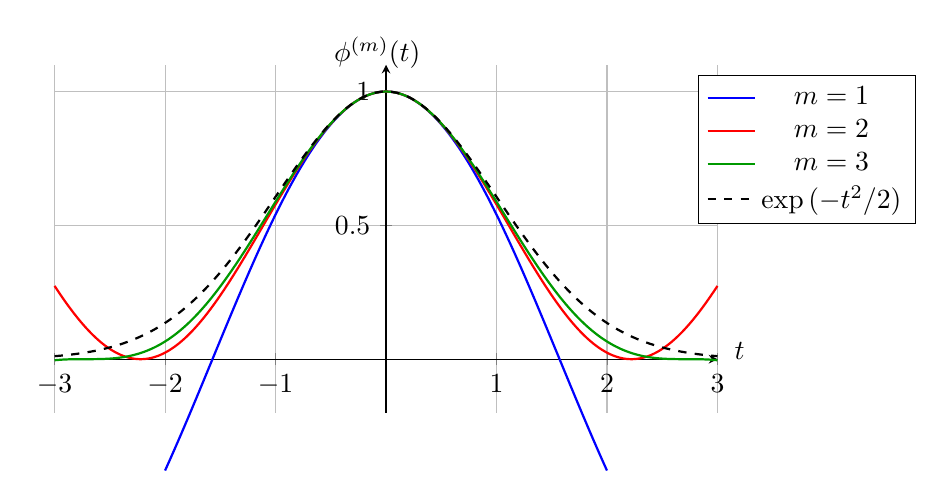
\begin{tikzpicture}
			\begin{axis}[
			width=10cm,
			height=6cm,
			xlabel={},
			ylabel={},
			legend style={at={(0.97,0.97)}, anchor=north west},
			domain=-3:3,
			ylabel style={
			yshift=10pt   % shift label up by 10pt
			},
			samples=400,
			ymin=-0.2, ymax=1.1,
			axis lines=middle,
			clip=false,
			grid=both,
			]
			\addplot[thick, blue,domain=-2:2] {cos(x/sqrt(1) r)^1};
			\addlegendentry{$m=1$}
			\addplot[thick, red] {cos(x/sqrt(2) r)^2};
			\addlegendentry{$m=2$}
			\addplot[thick, green!60!black] {cos(x/sqrt(3) r)^3};
			\addlegendentry{$m=3$}
			\addplot[thick, dashed, black] {exp(-x^2/2)};
			\addlegendentry{$\exp\,(-t^2/2)$}
			\node[anchor=south, rotate=0] at (axis cs:-0.08,1.05) {$\phi^{(m)}(t)$};
			\node[anchor=north, rotate=0] at (axis cs: 3.2,0.1) {$t$};
			\end{axis}
			\end{tikzpicture}
%			\caption{\Gls{characteristicfunc}s of normalized sums of \gls{iid} \gls{rv}s $x^{(\sampleidx)} \in \{-1,1\}$ 
%			for $\sampleidx=1,\ldots,\samplesize$ compared to the Gaussian limit.}
		\end{figure}
		\foreignlanguage{greek}{Βλέπε επίσης:} \gls{iid}, \gls{rv}, \gls{mean}, \gls{variance}, \gls{gaussrv}, \gls{characteristicfunc}, \gls{fixedpointiter}, \gls{generalization}, .},
	first={central limit theorem (CLT)},
	text={CLT}
}

\newglossaryentry{GaussProc}
{name={Gaussian process (GP)}, 
  description={A \index{Gaussian process (GP)}GP is a collection of \gls{rv}s 
  	$\{f(\featurevec)\}_{\featurevec \in \featurespace}$ indexed by input values $\featurevec$ 
  	from some input space $\featurespace$ such that, for any finite subset 
  	$\featurevec^{(1)}, \ldots, \featurevec^{(\samplesize)} \in \featurespace$, 
  	the corresponding \gls{rv}s $f(\featurevec^{(1)}, \ldots, \featurevec^{(\samplesize)})$ have a joint 
  	multivariate Gaussian distribution
  	\[
  	\left( f(\featurevec^{(1)}, \ldots, \featurevec^{(\samplesize)} \right) \sim \mathcal{N}(\boldsymbol{\mu}, \mathbf{K}).
  	\]
  	For a fixed input space $\featurespace$, a GP is fully specified (or parameterized) by: 1) a \gls{mean} \gls{function} $\mu(\featurevec) = \expect\{ f(\featurevec)\}$;
  	and 2) a \gls{covariance} \gls{function} $\kernelmap{\featurevec}{\featurevec'}= \expect\{ \big(f(\featurevec)-\mu(\featurevec)\big) \big(f(\featurevec')-\mu(\featurevec')\big) \big\}$.\\
  	Example:  We can interpret the temperature distribution across Finland (at a specific 
  	point in time) as the \gls{realization} of a GP $f(\featurevec)$, where each input $\featurevec = (\text{lat}, \text{lon})$ 
  	denotes a geographic location. Temperature observations from \gls{fmi} weather stations provide 
  	\gls{sample}s of $f(\featurevec)$ at specific locations (see Fig. \ref{fig_gp_FMI_dict}). A GP allows us to 
  	predict the temperature nearby \gls{fmi} weather stations and to quantify the \gls{uncertainty} 
  	of these \gls{prediction}s. 
  	\begin{figure}[H]
  	\begin{center}
  	\begin{tikzpicture}
	\begin{axis}[
	axis equal,
	hide axis,
	scale=1.2,
	xmin=17, xmax=32,
	ymin=55, ymax=71,
%	width=15cm,
%	height=20cm,
	clip=true
	]
	% --- Finland border (polyline) ---
	\addplot[
	color=black,
	thick
	] table [x=lon, y=lat, col sep=comma] {../../assets/finland_border.csv};
	% --- FMI sample stations ---
	\addplot[
	only marks,
	mark=*,
	mark options={fill=blue},
	color=black
	] table [x=lon, y=lat, col sep=comma] {../../assets/fmi_stations_subset.csv};
	% Draw manual axes
	\draw[->, thick] (axis cs:19,59) -- (axis cs:25.5,59) node[anchor=west] {lon};
	\draw[->, thick] (axis cs:19,59) -- (axis cs:19,65.5) node[anchor=south] {lat};
	\end{axis}
	\end{tikzpicture}
	\vspace*{-15mm}
	\end{center}
	\caption{We can interpret the temperature distribution over Finland as a \gls{realization} 
	of a GP indexed by geographic coordinates and sampled at \gls{fmi} weather stations (indicated by 
	blue dots). \label{fig_gp_FMI_dict}}
	\end{figure}
	\foreignlanguage{greek}{Βλέπε επίσης:} \gls{rv}, \gls{mean}, \gls{function}, \gls{covariance}, \gls{realization}, 
	\gls{fmi}, \gls{sample}, \gls{uncertainty}, \gls{prediction}. }, 
  first={Gaussian process}, 
  text = {GP}
}

\newglossaryentry{stability}
{name={stability},
	description={Stability\index{stability} is a desirable property of an \gls{ml} method $\algomap$ that maps a 
		\gls{dataset} $\dataset$ (e.g., a \gls{trainset}) to an output $\algomap(\dataset)$. The output 
		$\algomap(\dataset)$ can be the learned \gls{modelparams} or the \gls{prediction} delivered 
		by the trained \gls{model} for a specific \gls{datapoint}. Intuitively, $\algomap$ is 
		stable if small changes in the input \gls{dataset} $\dataset$ lead to small changes in the 
		output $\algomap(\dataset)$. Several formal notions of stability exist that enable bounds 
		on the \gls{generalization} error or \gls{risk} of the method (see \cite[Ch.~13]{ShalevMLBook}).
		To build intuition, consider the three \gls{dataset}s depicted in Fig. \ref{fig_three_data_stability_dict}, each 
		of which is equally likely under the same \gls{data}-generating \gls{probdist}. Since the 
		optimal \gls{modelparams} are determined by this underlying \gls{probdist}, an accurate 
		\gls{ml} method $\algomap$ should return the same (or very similar) output $\algomap(\dataset)$ 
		for all three \gls{dataset}s. In other words, any useful $\algomap$ must be robust to 
		variability in \gls{sample} \gls{realization}s from the same \gls{probdist}, i.e., it must be stable. 
		\begin{figure}[H]
			\centering
			\begin{tikzpicture}
				\begin{axis}[
				%title={Stem Plots of 3 Datasets},
				    axis lines=none,
					xlabel={$\sampleidx$},
					ylabel={},
					legend pos=north west,
					ymin=0, ymax=10,
					xtick={1,2,3,4,5},
				%	ymajorgrids=true,
					grid style=dashed,
					every axis plot/.append style={very thick}
					]
					% Dataset 1
					\addplot+[only marks,mark=*] coordinates {
						(1,2) (2,4) (3,3) (4,5) (5,7)
					};
				%	\addlegendentry{$\dataset^{(*)}$}
					% Dataset 2
					\addplot+[only marks,mark=square*] coordinates {
						(1,3) (2,2) (3,6) (4,4) (5,5)
					};
				%	\addlegendentry{$\dataset^{(\square)}$}
					% Dataset 3
					\addplot+[only marks,mark=triangle*] coordinates {
						(1,5) (2,7) (3,4) (4,6) (5,3)
					};
				%	\addlegendentry{$\dataset^{(\triangle)}$}
				\end{axis}
			\end{tikzpicture}
			\caption{Three \gls{dataset}s $\dataset^{(*)}$, $\dataset^{(\square)}$, and $\dataset^{(\triangle)}$, 
				each sampled independently from the same \gls{data}-generating \gls{probdist}. A stable \gls{ml} 
				method should return similar outputs when trained on any of these \gls{dataset}s. \label{fig_three_data_stability_dict}}
		\end{figure}
		\foreignlanguage{greek}{Βλέπε επίσης:} \gls{ml}, \gls{dataset}, \gls{trainset}, \gls{modelparams}, \gls{prediction}, 
		\gls{model}, \gls{datapoint}, \gls{generalization}, \gls{risk}, \gls{data}, \gls{probdist}, \gls{sample}, \gls{realization}.}, 
	first={stability}, 
	text={stability} 
}

\newglossaryentry{mab}
{name={multi-armed bandit (MAB)},
	description={A MAB\index{multi-armed bandit (MAB)} problem models 
		a repeated decision-making scenario in which, at each time step $\iteridx$, a learner must 
		choose one out of several possible actions, often referred to as arms, from a finite 
		set $\actionset$. Each arm $\action \in \actionset$ yields a \gls{stochastic} \gls{reward} $\reward^{(\action)}$ 
		drawn from an unknown \gls{probdist} with \gls{mean} $\mu^{(\action)}$. 
		The learner’s goal is to maximize the cumulative \gls{reward} over time by 
		strategically balancing exploration (gathering information about 
		uncertain arms) and exploitation (selecting arms known to perform well). 
		This balance is quantified by the notion of \gls{regret}, which measures the performance 
		gap between the learner's strategy and the optimal strategy that always selects the best arm. 
		MAB problems form a foundational \gls{model} in \gls{onlinelearning}, reinforcement learning, 
		and sequential experimental design \cite{Bubeck2012}.\\
		\foreignlanguage{greek}{Βλέπε επίσης:} \gls{stochastic}, \gls{reward}, \gls{probdist}, \gls{mean}, \gls{regret}, \gls{model}.},
	first={MAB},
	text={MAB}
}

\newglossaryentry{dualnorm}
{name={dual norm},
	description={Every \gls{norm} $\normgeneric{\cdot}{}$ defined on an \gls{euclidspace} $\mathbb{R}^{\dimlocalmodel}$ 
		has an associated dual \gls{norm}, which is denoted $\normgeneric{\cdot}{*}$ and defined as 
		$\normgeneric{\vy}{*} \defeq \sup_{\norm{\vx}{} \le 1} \vy\,^{T} \vx$. 
		The dual \gls{norm} measures the largest possible inner product between $\vy$ 
		and any vector in the unit ball of the original \gls{norm}. For further details, see 
		\cite[Sec.~A.1.6]{BoydConvexBook}.\\
		\foreignlanguage{greek}{Βλέπε επίσης:} \gls{norm}, \gls{euclidspace}.},
	first={dual norm},
	text={dual norm}
}

\newglossaryentry{distributedalgorithm}
{name={distributed algorithm},
	description={A\index{distributed algorithm} distributed \gls{algorithm} is an \gls{algorithm} designed for 
		a special type of computer: a collection of interconnected computing devices (or nodes). 
		These devices communicate and coordinate their local computations by exchanging 
		messages over a network \cite{IntroDistAlg}, \cite{ParallelDistrBook}. Unlike a classical \gls{algorithm}, 
		which is implemented on a single \gls{device}, a distributed \gls{algorithm} is 
		executed concurrently on multiple \gls{device}s with computational capabilities. 
		Similar to a classical \gls{algorithm}, a distributed \gls{algorithm} can be modeled as a 
		set of potential executions. However, each execution in the distributed setting involves 
		both local computations and message-passing events. A generic execution might look as 
		follows:
		\[
		\begin{array}{l}
			\text{Node 1: } {\rm input}_1, s_1^{(1)}, s_2^{(1)}, \ldots, s_{T_1}^{(1)}, {\rm output}_1; \\
			\text{Node 2: } {\rm input}_2, s_1^{(2)}, s_2^{(2)}, \ldots, s_{T_2}^{(2)}, {\rm output}_2; \\
			\quad \vdots \\
			\text{Node N: } {\rm input}_N, s_1^{(N)}, s_2^{(N)}, \ldots, s_{T_N}^{(N)}, {\rm output}_N.
		\end{array}
		\]
		Each \gls{device} $\nodeidx$ starts from its own local input and performs a sequence of 
		intermediate computations $s_{\iteridx}^{(\nodeidx)}$ at discrete time instants $\iteridx = 1, \dots, T_\nodeidx$. 
		These computations may depend on both: the previous local computations at the \gls{device} 
		and messages received from other \gls{device}s. One important application of distributed 
		\gls{algorithm}s is in \gls{fl} where a network of \gls{device}s collaboratively train a personal \gls{model} 
		for each \gls{device}.\\
		\foreignlanguage{greek}{Βλέπε επίσης:} \gls{algorithm}, \gls{device}, \gls{fl}, \gls{model}.},
	first={distributed algorithm}, 
	text={distributed algorithm}
}

\newglossaryentry{onlinelearning}
{name={online learning},
	description={Some \gls{ml} methods \index{online learning} are designed to process \gls{data} in a sequential 
		manner, updating their \gls{modelparams} one at a time, as new \gls{datapoint}s become available. 
		A typical example is time series data, such as daily \gls{minimum} and \gls{maximum} temperatures 
		recorded by an \gls{fmi} weather station. These values form a chronological sequence 
		of observations. In online learning, the \gls{hypothesis} (or its \gls{modelparams}) is refined 
		incrementally with each newly observed \gls{datapoint}, without revisiting past \gls{data}.  \\ 
		\foreignlanguage{greek}{Βλέπε επίσης:} \gls{ml}, \gls{data}, \gls{modelparams}, \gls{datapoint}, 
		\gls{fmi}, \gls{hypothesis}, \gls{onlineGD}, \gls{onlinealgorithm}.  },
	first={online learning},
	text={online learning} 
}

\newglossaryentry{onlinealgorithm}
{name={online algorithm},
	description={An\index{online algorithm} online \gls{algorithm} processes input \gls{data} incrementally, 
		receiving \gls{datapoint}s sequentially and making decisions or producing outputs (or decisions) immediately 
		without having access to the entire input in advance \cite{PredictionLearningGames}, \cite{HazanOCO}. 
		Unlike an offline \gls{algorithm}, which has the entire input available from the start, an online \gls{algorithm} 
		must handle \gls{uncertainty} about future inputs and cannot revise past decisions. Similar to an 
		offline \gls{algorithm}, we represent an online \gls{algorithm} formally as a collection of possible 
		executions. However, the execution sequence for an online \gls{algorithm} has a distinct structure as follows:
		$${\rm in}_{1}, s_1, {\rm out}_{1}, {\rm in}_{2}, s_2, {\rm out}_{2}, \ldots, {\rm in}_{T}, s_T, {\rm out}_{T}.$$ 
		Each execution begins from an initial state (i.e., \(\text{in}_{1}\)) and proceeds through alternating 
		computational steps, outputs (or decisions), and inputs. Specifically, at step \(\iteridx\), 
		the \gls{algorithm} performs a computational step \(s_{\iteridx}\), generates an output \(\text{out}_{\iteridx}\), 
		and then subsequently receives the next input (\gls{datapoint}) \(\text{in}_{\iteridx+1}\). A 
		notable example of an online \gls{algorithm} in \gls{ml} is \gls{onlineGD}, which incrementally 
		updates \gls{modelparams} as new \gls{datapoint}s arrive. 
					\\ 
		\foreignlanguage{greek}{Βλέπε επίσης:} \gls{algorithm}, \gls{data}, \gls{datapoint}, \gls{uncertainty}, \gls{ml}, 
		\gls{onlineGD}, \gls{modelparams}, \gls{onlinelearning}.},
	first={online algorithm},
	text={online algorithm} 
}

%\newglossaryentry{transparency}
%{name={transparency},
%	description={Transparency\index{transparency} is a key requirement for 
%		trustworthy \gls{ai} \cite{HLEGTrustworhtyAI}. In the context of ML methods, 
%		such as \gls{erm}-based methods, transparency is mainly used synonymously 
%		for \gls{explainability} \cite{gallese2023ai,JunXML2020}. However, in the wide 
%		context of \gls{ai} systems, transparency also includes providing information 
%		about limitations and reliability of the \gls{ai} system. As a point in case, \gls{logreg} provides a 
%		quantitative measure of the reliability of a \gls{classification} in the form of the value $|\hypothesis(\featurevec)|$. 
%		Transparency also includes the user interface, by requiring to clearly indicate when a user is 
%		interaction with an \gls{ai} system. Another component of transparency is the documentation 
%		of the system’s purpose, design choices, and intended use cases \cite{Shahriari2017,DatasheetData2021,10.1145/3287560.3287596}. },
%	first={transparency},text={transparency} 
%}

\newcommand{\gaussiancenter}{3}

\newglossaryentry{spectrogram}
{name={spectrogram},
	description={A\index{spectrogram} spectrogram represents the time-frequency distribution of the energy of a time signal $x(t)$.  
		Intuitively, it quantifies the amount of signal energy present within a specific time segment 
		$[t_{1},t_{2}] \subseteq \mathbb{R}$ and frequency interval $[f_{1},f_{2}]\subseteq \mathbb{R}$. 
		Formally, the spectrogram of a signal is defined as the squared magnitude of its 
		short-time Fourier transform (STFT) \cite{cohen1995time}.
        		Fig. \ref{fig:spectrogram_dict} depicts a time signal along with its spectrogram. 
		\begin{figure}[H]
			\centering
			\includegraphics[width=0.8\textwidth]{assets/spectrogram.png}
			\begin{minipage}{\textwidth}
				\vspace{3ex}
				\centering
				{\selectfont (a) \hspace{10em} (b)}
			\end{minipage}
			\caption{(a) A time signal consisting of two modulated Gaussian pulses. (b) An intensity 
			plot of the spectrogram.
			\label{fig:spectrogram_dict}}
		\end{figure}
        		The intensity plot of its spectrogram can serve as an image of a signal. A 
		simple recipe for audio signal \gls{classification} is to feed this signal image 
		into \gls{deepnet}s originally developed for image \gls{classification} and object detection \cite{Li:2022aa}. 
		It is worth noting that, beyond the spectrogram, several alternative representations exist 
		for the time-frequency distribution of signal energy \cite{TimeFrequencyAnalysisBoashash}, \cite{MallatBook}.\\
		\foreignlanguage{greek}{Βλέπε επίσης:} \gls{classification}, \gls{deepnet}.}, 
	first={spectrogram},
	text={spectrogram}
}

\newglossaryentry{gtvmin}
{name={generalized total variation minimization (GTVMin)},
	description={GTVMin\index{generalized total variation minimization (GTVMin)} is an instance of \gls{rerm} 
		using the \gls{gtv} of local \gls{modelparams} as a \gls{regularizer} \cite{ClusteredFLTVMinTSP}.\\
		\foreignlanguage{greek}{Βλέπε επίσης:} \gls{rerm}, \gls{gtv}, \gls{modelparams}, \gls{regularizer}.},
	first={generalized total variation minimization (GTVMin)},
	text={GTVMin} 
}

\newglossaryentry{modelinversion}
{name={model inversion},
  description={A\index{model inversion} \gls{model} inversion is a form of \gls{privattack} on a \gls{ml} system. 
  	An adversary seeks to infer \gls{sensattr}s of individual \gls{datapoint}s by exploiting partial access 
  	to a trained \gls{model} $\learnthypothesis \in \hypospace$. This access typically consists of 
  	querying the \gls{model} for \gls{prediction}s $\learnthypothesis(\featurevec)$ using carefully chosen inputs. 
  	Basic \gls{model} inversion techniques have been demonstrated in the context of facial image 
  	\gls{classification}, where images are reconstructed using the (\gls{gradient} of) \gls{model} outputs 
  	combined with auxiliary information such as a person’s name \cite{Fredrikson2015}.
   	\begin{figure}[H]
	\begin{center}
	\begin{tikzpicture}[scale=1.5]
  		% Axes
  		\draw[->] (-0.5,0) -- (5.5,0) node[right] {face image $\featurevec$};
  		\draw[->] (0,-0.2) -- (0,2.5) node[above] {name};
  		% Sigmoid-like curve
  		\draw[thick, domain=0.5:5, samples=100, smooth, variable=\x, name path=sigmoid] 
  		plot ({\x}, {2/(1 + exp(-3*(\x - 3)))});
  		%\node at (5.1, 0.2) {\small (e.g., face photo)};
  		% Highlight point
  		\def\xval{3}
  		\pgfmathsetmacro{\yval}{2/(1 + exp(-3*(\xval - 3)))}
  		% Ruler lines
  		\draw[dashed] (\xval,0) -- (\xval,\yval);
  		\draw[dashed] (0,\yval) -- (\xval,\yval);
  		% Filled circle
  		\filldraw[fill=blue!20, draw=blue] (\xval,\yval) circle (0.1);
  		\node[anchor=south east] at (-0.1,\yval) {\footnotesize ``Alexander Jung''};
  		% Axis labels with image
  		\node[anchor=north] at (\xval,-0.25) {\includegraphics[width=1cm]{assets/AlexanderJung.jpg}}; % Replace 'face.jpg' with your image
  		% Label on curve
  		\node[above right] at (4,2.2) {trained \gls{model} $\learnthypothesis$};
  	\end{tikzpicture}
  	\end{center} 
	\caption{Model inversion techniques implemented in the context of facial image classification. \label{fig_model_inv_dict}}
	\end{figure}
  	\foreignlanguage{greek}{Βλέπε επίσης:} \gls{model}, \gls{privattack}, \gls{ml}, \gls{sensattr}, \gls{datapoint}, 
	\gls{prediction}, \gls{classification}, \gls{gradient}, \gls{trustAI}, \gls{privprot}. },
  first={model inversion},
  text={model inversion}
}

\newglossaryentry{bagging}
{name={bagging (or bootstrap aggregation)},
	description={Bagging\index{bagging (or bootstrap aggregation)} (or bootstrap aggregation) 
		is a generic technique to improve (the \gls{robustness} of) a given \gls{ml} method. 
		The idea is to use the \gls{bootstrap} to generate perturbed copies of a given \gls{dataset} 
		and to learn a separate \gls{hypothesis} for each copy. We then predict the 
		\gls{label} of a \gls{datapoint} by combining or aggregating the individual \gls{prediction}s 
		of each separate \gls{hypothesis}. For \gls{hypothesis} \gls{map}s delivering numeric \gls{label} 
		values, this aggregation could be implemented by computing the average of individual 
		\gls{prediction}s.\\
		\foreignlanguage{greek}{Βλέπε επίσης:} \gls{robustness}, \gls{ml}, \gls{bootstrap}, \gls{dataset}, 
		\gls{hypothesis}, \gls{label}, \gls{datapoint}, \gls{prediction}, \gls{map}.},
	first={bagging (or bootstrap aggregation)},
	text={bagging}  
}

\newglossaryentry{onlineGD}
{name={online gradient descent (online GD)}, 
	description={Consider \index{online gradient descent (online GD)} an \gls{ml} method that learns \gls{modelparams} 
		$\weights$ from some \gls{paramspace} $\paramspace \subseteq \mathbb{R}^{\dimlocalmodel}$. 
		The learning process uses \gls{datapoint}s $\datapoint^{(\timeidx)}$ that arrive at consecutive time-instants $\timeidx=1, 2, \dots$. 
		Let us interpret the \gls{datapoint}s $\datapoint^{(\timeidx)}$ as \gls{iid} copies 
		of an \gls{rv} $\datapoint$. The \gls{risk} $\expect\{ \lossfunc{\datapoint}{\weights} \}$ of a 
		\gls{hypothesis} $\hypothesis^{(\weights)}$ can then (under mild conditions) be obtained as the limit 
		$\lim_{T\rightarrow \infty} (1/T)\sum_{\timeidx=1}\,^{T} \lossfunc{\datapoint^{(\timeidx)}}{\weights}$. 
		We might use this limit as the \gls{objfunc} for learning the \gls{modelparams} $\weights$. 
		Unfortunately, this limit can only be evaluated if we wait infinitely long in order to collect all \gls{datapoint}s. 
		Some \gls{ml} applications require methods that learn online: as soon as a new \gls{datapoint} $\datapoint^{(\timeidx)}$ 
		arrives at time $\timeidx$, we update the current \gls{modelparams} $\weights^{(\timeidx)}$. Note that 
		the new \gls{datapoint} $\datapoint^{(\timeidx)}$ contributes the component $\lossfunc{\datapoint^{(\timeidx)}}{\weights}$ 
		to the \gls{risk}. As its name suggests, online \gls{gd} updates $\weights^{(\timeidx)}$ via a (projected) \gls{gradstep}
		\begin{equation} 
		\label{equ_def_ogd_dict}
 		\weights^{(\timeidx+1)} \defeq \projection{\paramspace}{\weights^{(\timeidx)} - \lrate_{\timeidx} \nabla_{\weights} \lossfunc{\datapoint^{(\timeidx)}}{\weights}}. 
		\end{equation} 
		Note that \eqref{equ_def_ogd_dict} is a \gls{gradstep} for the current component $\lossfunc{\datapoint^{(\timeidx)}}{\cdot}$ 
		of the \gls{risk}. The update \eqref{equ_def_ogd_dict} ignores all the previous components $\lossfunc{\datapoint^{(\timeidx')}}{\cdot}$, 
		for $\timeidx' < \timeidx$. It might therefore happen that, compared to $\weights^{(\timeidx)}$, the updated \gls{modelparams} 
		$\weights^{(\timeidx+1)}$ increase the retrospective average \gls{loss} $\sum_{\timeidx'=1}^{\timeidx-1} \lossfunc{\datapoint^{(\timeidx')}}{\cdot}$. 
		However, for a suitably chosen \gls{learnrate} $\lrate_{\timeidx}$, online \gls{gd} can be shown 
		to be optimal in practically relevant settings. By optimal, we mean that the \gls{modelparams} 
		$\weights^{(T+1)}$ delivered by online \gls{gd} after observing $T$ \gls{datapoint}s $\datapoint^{(1)}, \ldots, \datapoint^{(T)}$ 
		are at least as good as those delivered by any other learning method \cite{HazanOCO}, \cite{GDOptimalRakhlin2012}. 
		\begin{figure}[H]
			\begin{center}
			\begin{tikzpicture}[x=1.5cm,scale=1.5, every node/.style={font=\footnotesize}]
			\draw[->] (0.5, 0) -- (5.5, 0) node[below] {};
			\foreach \x in {1, 2, 3, 4, 5} {
				\draw (\x, 0.1) -- (\x, -0.1) node[below] {$t=\x$};
			}
			\foreach \x/\y in {1/2.5, 2/1.8, 3/2.3, 4/1.5, 5/2.0} {
				\fill[black] (\x, \y) circle (2pt) node[above right] {$\datapoint^{(\x)}$};
			}
			\foreach \x/\y in {1/1.0, 2/1.6, 3/1.8, 4/2.2, 5/1.9} {
				\fill[blue] (\x, \y) circle (2pt) node[below left] {$\weights^{(\x)}$};
			}
			\foreach \x/\y/\z in {1/2.5/1.0, 2/1.8/1.6, 3/2.3/2.0, 4/1.5/1.8, 5/2.0/1.9} {
				\draw[dashed, gray] (\x, \y) -- (\x, \z);
			}
			\end{tikzpicture}
			\end{center} 
			\caption{An instance of online \gls{gd} that updates the \gls{modelparams} $\weights^{(\timeidx)}$ 
			using the \gls{datapoint} $\datapoint^{(\timeidx)} = \feature^{(\timeidx)}$ arriving at time $\timeidx$. 
			This instance uses the \gls{sqerrloss} $\lossfunc{\datapoint^{(\timeidx)}}{\weight} = (\feature^{(\timeidx)} - \weight)^{2}$. }
		\end{figure}
		\foreignlanguage{greek}{Βλέπε επίσης:} \gls{ml}, \gls{modelparams}, \gls{paramspace}, \gls{datapoint}, 
		\gls{iid}, \gls{rv}, \gls{risk}, \gls{hypothesis}, \gls{objfunc}, \gls{gd}, \gls{gradstep}, \gls{loss}, \gls{learnrate}, \gls{sqerrloss}.},
	first={online gradient descent (online GD)},
	text={online GD} 
}

\newglossaryentry{ppca}
{name={probabilistic principal component analysis (PPCA)}, 
	description={PPCA\index{probabilistic principal component analysis (PPCA)}
		extends basic \gls{pca} by using a \gls{probmodel} for \gls{datapoint}s. The \gls{probmodel} 
		of PPCA reduces the task of dimensionality reduction to an estimation problem that can be 
		solved using \gls{em} \cite{TippingProbPCA}.\\
		\foreignlanguage{greek}{Βλέπε επίσης:} \gls{pca}, \gls{probmodel}, \gls{datapoint}, \gls{em}.},
	first={probabilistic principal component analysis (PPCA)},
	text={PPCA}
}

\newglossaryentry{gmm}
{name={Gaussian mixture model (GMM)}, 
	description={A GMM\index{Gaussian mixture model (GMM)} 
		is a particular type of \gls{probmodel} for a numeric vector $\featurevec$ (e.g., 
		the \gls{feature}s of a \gls{datapoint}). Within a GMM, the vector $\featurevec$ is drawn from a randomly 
		selected \gls{mvndist} $p^{(\clusteridx)} = \mvnormal{\meanvec{\clusteridx}}{\covmtx{\clusteridx}}$ with 
		$\clusteridx = I$. The index $I \in \{1, \ldots, \nrcluster\}$ is an \gls{rv} with probabilities $\prob{I=\clusteridx} = p_{\clusteridx}$.
	     	Note that a GMM is parametrized by the \gls{probability} $p_{\clusteridx}$, the 
		\gls{mean} vector $\clustermean^{(\clusteridx)}$, and the \gls{covmtx} $\bf\Sigma^{(\clusteridx)}$ for each $\clusteridx=1, \ldots, \nrcluster$. 
		GMMs are widely used for \gls{clustering}, density estimation, and as a generative \gls{model}.\\
		\foreignlanguage{greek}{Βλέπε επίσης:} \gls{probmodel}, \gls{feature}, \gls{datapoint}, \gls{mvndist}, \gls{rv}, 
		\gls{mean}, \gls{covmtx}, \gls{clustering}, \gls{model}. },
	first={Gaussian mixture model (GMM)},
	text={GMM} 
}
	 
\newglossaryentry{em}
{name={expectation-maximization (EM)}, 
	description={\index{expectation-maximization (EM)} 
		Consider a \gls{probmodel} $\prob{\datapoint; \weights}$ for the \gls{datapoint}s $\dataset$ generated in some 
		\gls{ml} application. The \gls{maxlikelihood} estimator for the \gls{modelparams} $\weights$ is obtained by maximizing 
		$\prob{\dataset; \weights}$. However, the resulting \gls{optproblem} might be computationally 
		challenging. EM approximates the \gls{maxlikelihood} estimator by introducing a latent 
		\gls{rv} $\vz$ such that maximizing $\prob{\dataset,\vz; \weights}$ would be 
		easier \cite{hastie01statisticallearning}, \cite{BishopBook}, \cite{GraphModExpFamVarInfWainJor}. Since we 
		do not observe $\vz$, we need to estimate it from the observed \gls{dataset} $\dataset$ 
		using a conditional \gls{expectation}. The resulting estimate $\widehat{\vz}$ is then used to 
		compute a new estimate $\widehat{\weights}$ by solving $\max_{\weights} \prob{\dataset, \widehat{\vz}; \weights}$. 
		The crux is that the conditional \gls{expectation} $\widehat{\vz}$ depends on the \gls{modelparams} $\widehat{\weights}$, 
		which we have updated based on $\widehat{\vz}$. Thus, we have to re-calculate $\widehat{\vz}$, 
		which, in turn, results in a new choice $\widehat{\weights}$ for the \gls{modelparams}. In practice, 
		we repeat the computation of the conditional \gls{expectation} (i.e., the E-step) and the update 
		of the \gls{modelparams} (i.e., the M-step) until some \gls{stopcrit} is met.\\
		\foreignlanguage{greek}{Βλέπε επίσης:} \gls{probmodel}, \gls{datapoint}, \gls{ml}, \gls{maxlikelihood}, \gls{modelparams}, 
		\gls{optproblem}, \gls{rv}, \gls{dataset}, \gls{expectation}, \gls{stopcrit}.},
	first={EM},
  	text={EM}
}

\newglossaryentry{highdimregime}
{name={high-dimensional regime}, 
	description={The\index{high-dimensional regime} 
		high-dimensional regime of \gls{erm} is characterized by the \gls{effdim} of the \gls{model} 
		being larger than the \gls{samplesize}, i.e., the number of (labeled) \gls{datapoint}s in the \gls{trainset}. 
		For example, \gls{linreg} methods operate in the high-dimensional regime whenever the number $\featuredim$ of \gls{feature}s 
		used to characterize \gls{datapoint}s exceeds the number of \gls{datapoint}s in the \gls{trainset}. 
		Another example of \gls{ml} methods that operate in the high-dimensional regime is large \gls{ann}s, which have 
		far more tunable \gls{weights} (and bias terms) than the total number of \gls{datapoint}s in the \gls{trainset}. 
		High-dimensional statistics is a recent main thread of \gls{probability} theory that studies the 
		behavior of \gls{ml} methods in the high-dimensional regime \cite{Wain2019}, \cite{BuhlGeerBook}.\\
		\foreignlanguage{greek}{Βλέπε επίσης:} \gls{erm}, \gls{effdim}, \gls{model}, \gls{samplesize}, \gls{datapoint}, \gls{trainset}, 
		\gls{linreg}, \gls{feature}, \gls{ml}, \gls{ann}, \gls{weights}, \gls{probability}, \gls{overfitting}, \gls{regularization}.},
   	first={high-dimensional regime},
   	text={high-dimensional regime}
}
	
\newglossaryentry{cfl}
{name={clustered federated learning (CFL)}, 
	description={CFL\index{clustered federated learning (CFL)} trains \gls{localmodel}s for the 
 		\gls{device}s in a \gls{fl} application by using a \gls{clustasspt}, i.e., the \gls{device}s 
 		of an \gls{empgraph} form \gls{cluster}s. Two \gls{device}s in the same \gls{cluster} generate 
 		\gls{localdataset}s with similar statistical properties. CFL pools the \gls{localdataset}s of \gls{device}s 
 		in the same \gls{cluster} to obtain a \gls{trainset} for a \gls{cluster}-specific \gls{model}. 
 		\Gls{gtvmin} clusters \gls{device}s implicitly by enforcing approximate similarity of \gls{modelparams} 
 		across well-connected nodes of the \gls{empgraph}.\\
		\foreignlanguage{greek}{Βλέπε επίσης:}  \gls{localmodel}, \gls{device}, \gls{fl}, \gls{clustasspt}, \gls{empgraph}, 
		\gls{cluster}, \gls{localdataset}, \gls{trainset}, \gls{model}, \gls{gtvmin}, \gls{modelparams}, \gls{graphclustering}.}, 
	first={clustered federated learning (CFL)},
	text={CFL} 
}

\newglossaryentry{algconn}
{name={algebraic connectivity},
	description={The\index{algebraic connectivity} algebraic connectivity of an undirected \gls{graph} 
		is the second-smallest \gls{eigenvalue} $\eigval{2}$ of its \gls{LapMat}. A \gls{graph} is connected if and only if 
		$\eigval{2} >0$.\\
		\foreignlanguage{greek}{Βλέπε επίσης:} \gls{graph}, \gls{eigenvalue}, \gls{LapMat}.},
	first={algebraic connectivity},
	text={algebraic connectivity}
}

\newglossaryentry{cfwmaxmin}
{name={Courant–Fischer–Weyl min-max characterization}, 
	description={Consider\index{Courant–Fischer–Weyl min-max characterization} a \gls{psd} 
		matrix $\mQ \in \mathbb{R}^{\nrfeatures \times \nrfeatures}$ with \gls{evd} (or spectral decomposition), i.e.,
		$$\mQ = \sum_{\featureidx=1}^{\nrfeatures} \eigval{\featureidx} \vu^{(\featureidx)} \big(  \vu^{(\featureidx)}  \big)\,^{T}.$$ 
		Here, we use the ordered (in ascending order) \gls{eigenvalue}s 
		\begin{equation}
			\nonumber
			 \eigval{1}  \leq  \ldots \leq \eigval{\nrnodes}. 
		\end{equation}
		The Courant–Fischer–Weyl min-max characterization \cite[Th. 8.1.2]{GolubVanLoanBook} 
		represents the \gls{eigenvalue}s of $\mQ$ as the solutions to certain \gls{optproblem}s.\\
		\foreignlanguage{greek}{Βλέπε επίσης:} \gls{psd}, \gls{evd}, \gls{eigenvalue}, \gls{optproblem}.}, 
	first={Courant–Fischer–Weyl min-max characterization (CFW)}, 
	text={CFW}
}

\newglossaryentry{netexpfam}
{name={networked exponential families (nExpFam)}, 
	description={A\index{networked exponential families (nExpFam)} collection of exponential 
		families, each of them assigned to a node of an \gls{empgraph}. The \gls{modelparams} are coupled 
	   	via the network structure by requiring them to have a small \gls{gtv} \cite{JungNetExp2020}.\\
	   	\foreignlanguage{greek}{Βλέπε επίσης:} \gls{empgraph}, \gls{modelparams}, \gls{gtv}.},
	  first={networked exponential family (nExpFam)},
	  text={nExpFam}  
}

 \newglossaryentry{rlm}
 {name={regularized loss minimization (RLM)},
 	description={See\index{regularized loss minimization (RLM)} \gls{rerm}.},
 	text={RLM}
 }
 
\newglossaryentry{datapoisoning}
{name={data poisoning}, 
 	description={\Gls{data}\index{data poisoning} poisoning refers to the intentional manipulation 
  		(or fabrication) of \gls{datapoint}s to steer the training of an \gls{ml} \gls{model} \cite{Liu2021}, \cite{PoisonGAN}. 
  		\Gls{data} poisoning \gls{attack}s take various forms, including the following:
  		%\begin{itemize}
  		%	\item \Gls{backdoor} \gls{attack}s: Implanting triggers into training \gls{data}, so that the trained \gls{model} 
  		%	behaves normally on typical \gls{featurevec}s but misclassifies a \gls{featurevec} with a trigger pattern.
  		%	\item \Gls{dosattack}: Degrading overall performance of the trained \gls{model} by injecting mislabeled or 
  		%	adversarial examples to prevent effective learning.
  		%\end{itemize}
		\Gls{data} poisoning is particularly concerning in decentralized or distributed \gls{ml} settings (such as \gls{fl}), 
		where training \gls{data} cannot be centrally verified. \\
		\foreignlanguage{greek}{Βλέπε επίσης:} \gls{data}, \gls{datapoint}, \gls{ml}, \gls{model}, \gls{attack}, \gls{backdoor}, 
		\gls{featurevec}, \gls{dosattack}, \gls{fl}, \gls{trustAI}.},
	first={data poisoning},
	text={data poisoning}
}

\newglossaryentry{epigraph}
{name={epigraph},
  description={The epigraph\index{epigraph} of a real-valued \gls{function} $f : \mathbb{R}^n \to \mathbb{R} \cup \{+\infty\}$ 
  	is the set of points lying on or above its \gls{graph}:
		\[
		\operatorname{epi}(f) = \left\{ (\mathbf{x}, t) \in \mathbb{R}^n \times \mathbb{R} \,\middle|\, f(\mathbf{x}) \leq t \right\}.
		\]
		A \gls{function} is \gls{convex} if and only if its epigraph is a \gls{convex} set \cite{BoydConvexBook}, \cite{BertCvxAnalOpt}.
		\begin{figure}[H]
			\centering
			\begin{tikzpicture}[scale=1.0]
				\begin{axis}[
					axis lines = middle,
					xlabel = $x$,
					ylabel = {},
					xmin=-2, xmax=2,
					ymin=0, ymax=4.5,
					samples=100,
					domain=-1.5:1.5,
					thick,
					width=8cm,
					height=6cm,
					grid=none,
					axis on top,
					]
					% Function
					\addplot [blue, thick, domain=-1.5:1.5] {x^2} node [pos=0.85, anchor=south west, xshift=5pt] {$f(x)$};
					% Epigraph shading
					\addplot [
					name path=f,
					draw=none,
					ytick=\empty,
					domain=-1.5:1.5,
					] {x^2};
					\path[name path=top] (axis cs:-1.5,4) -- (axis cs:1.5,4);
					\addplot [
					blue!20,
					opacity=0.6,
					draw=none,
					] fill between [
					of=f and top,
					soft clip={domain=-1.5:1.5},
					];
					    \node[font=\small] at (axis cs:-1.0,2.3) {$\operatorname{epi}(f)$};
				%	\node[align=center, fill=white, draw=black, rounded corners, font=\small] at (axis cs:0.5,3.5) {Epigraph\\$\{(x,t) \mid f(x) \le t\}$};
				\end{axis}
			\end{tikzpicture}
			\caption{Epigraph of the \gls{function} $f(x) = x^2$ (i.e., shaded area).}
		\end{figure}
		\foreignlanguage{greek}{Βλέπε επίσης:} \gls{function}, \gls{graph}, \gls{convex}.},
	first={epigraph},
	text={epigraph},
	user1={\foreignlanguage{greek}{επίγραμμα}}, %nominative
	user2={\foreignlanguage{greek}{επίγραμμά}} %nominativeoraccusativedoublestress
}

\newglossaryentry{geometricmedian}
{name={geometric median (GM)},
	description={The GM\index{geometric median (GM)} of a set of input vectors $\vx^{(1)}, \ldots, \vx^{(\samplesize)}$ 
		in $\mathbb{R}^{\dimlocalmodel}$ is a point $\vz \in \mathbb{R}^{\dimlocalmodel}$ that 
		minimizes the sum of distances to the vectors \cite{BoydConvexBook} such that
		\begin{equation} 
			\label{equ_geometric_median_dict}
		\vz \in \aargmin_{\vy \in \mathbb{R}^{\dimlocalmodel}} \sum_{\sampleidx=1}^{\samplesize} \normgeneric{\vy - \vx^{(\sampleidx)}}{2}.
		\end{equation} 
		Fig. \ref{opt_cond_GM_dict} illustrates a fundamental property of the GM:
		If $\vz$ does not coincide with any of the input vectors, then the unit vectors pointing 
		from $\vz$ to each $\vx^{(\sampleidx)}$ must sum to zero—this is the zero-\gls{subgradient}  
		(optimality) condition of \eqref{equ_geometric_median_dict}. It turns out that the solution to 
		\eqref{equ_geometric_median_dict} cannot be arbitrarily pulled away from trustworthy input vectors as long as they 
		are the majority \cite[Th. 2.2]{Lopuhaae1991}.
	  	\begin{figure}[H]
  		\begin{center}
			\begin{tikzpicture}[scale=2, thick, >=stealth]
%				% Central model w
				\coordinate (w) at (3,0);
				\fill (w) circle (1.2pt) node[below right] {$\vz$};
% Clean nodes
				\coordinate (w2) at (0.5,0.3);
				\coordinate (w3) at (0.7,0.7);
				\fill (w2) circle (1pt) node[above left] {$\vx^{(1)}$};
				\fill (w3) circle (1pt) node[above left] {$\vx^{(2)}$};
			    \node[anchor=west] at ($(w2) +(-0.2,0.9)$) {\textbf{clean}};
%				% Dashed lines from w to good nodes
				\draw[dashed] (w) -- (w2);
				\draw[dashed] (w) -- (w3);
%				% Draw unit vectors (scaled to 1cm)
				\draw[->, thick, red] (w) -- ($(w)!1cm!(w2)$) ;
				\draw[->, thick, red] (w) -- ($(w)!1cm!(w3)$) node[pos=0.9, right,yshift=7pt] {$\frac{\vx^{(2)}- \vz}{\normgeneric{\vx^{(2)}-\vz}{2}}$};
%				\node at (-0.2,1.4) {\textbf{Clean}};
				\coordinate (w4) at (5,0.2);
				\node at (5,0.6) {\textbf{perturbed}};
				\fill (w4) circle (1pt) node[below left] {$\vx^{(3)}$};
				\draw[->, thick, red] (w) -- ($(w)!1cm!(w4)$) ;
%		% Optional dotted line from w to bad
		\end{tikzpicture}
		\caption{\label{opt_cond_GM_dict}
			Consider a solution $\vz$ of \eqref{equ_geometric_median_dict} that does not coincide 
			with any of the input vectors. The optimality condition for \eqref{equ_geometric_median_dict} 
			requires that the unit vectors from $\vz$ to the input vectors sum to zero.}
		\end{center}
		\end{figure}
		See also: \gls{subgradient}. },
	first={geometric median},
	text={GM}
}

\newglossaryentry{FedRelax}
{name={FedRelax},
	description={An\index{FedRelax} \gls{fl} \gls{distributedalgorithm}. \\ 
		See also: \gls{fl}, \gls{distributedalgorithm}.},
	first={FedRelax},
	text={FedRelax}
} 

\newglossaryentry{fedavg}
{name={FedAvg},
	description={FedAvg\index{FedAvg} refers to a family of iterative \gls{fl} \gls{algorithm}s. 
		It uses a server-client setting and alternates between client-wise \gls{localmodel}s
		re-training, followed by the aggregation of updated \gls{modelparams} at the server 
		\cite{pmlr-v54-mcmahan17a}. The local update at client $\nodeidx=1, \ldots, \nrnodes$ 
		at time $\iteridx$ starts from the current \gls{modelparams} $\weights^{(\iteridx)}$ provided 
		by the server and typically amounts to executing few iterations of \gls{stochGD}. After completing the 
		local updates, they are aggregated by the server (e.g., by averaging them). 
		Fig. \ref{fig_single_iteration_fedavg_dict} illustrates the execution of a single 
		iteration of FedAvg. 
		\begin{figure}[H]
			\begin{center}
			\begin{tikzpicture}[>=Stealth, node distance=1cm and 1.5cm, every node/.style={font=\small}]
			% Styles
			\tikzstyle{server} = [circle, fill=black, minimum size=6pt, inner sep=0pt]
			\tikzstyle{client} = [circle, draw=black, minimum size=6pt, inner sep=0pt]
			% Time step labels
			\node (label1) at (0,3.5) {broadcast};
			\node[right=2.5cm of label1] (label2) {local update};
			\node[right=2.5cm of label2] (label3) {aggregate};
			% Time step k
			\node[server] (s1) at (label1 |- 0,2.5) {};
			\node[client] (c1l) at ($(s1) + (-1cm,-1cm)$) {};
			\node[client] (c1r) at ($(s1) + (1cm,-1cm)$) {};
			\node[] (dots1) at ($(s1) + (0cm,-1cm)$) {\ldots};
			\draw[->] (s1) -- (c1l) node[midway,left] {$\weights^{(\iteridx)}$};
			\draw[->] (s1) -- (c1r) node[midway,right] {$\weights^{(\iteridx)}$};
			\draw[->] (s1) -- (dots1);
			% Time step k+1 (local updates)
			\node[server] (s2) at (label2 |- 0,2.5) {};
			\node[client] (c2l) at ($(s2) + (-1cm,-1cm)$) {};
			\node[client] (c2r) at ($(s2) + (1cm,-1cm)$) {};
			\node[] (dots2) at ($(s2) + (0cm,-1cm)$) {\ldots};
			\node[below=0.2cm of c2l] {$\localparamsiter{\iteridx}{1}$};
			\node[below=0.2cm of c2r] {$\localparamsiter{\iteridx}{\nrnodes}$};
			% Time step k+2 (aggregation)
			\node[server] (s3) at (label3 |- 0,2.5) {};
			\node[above=0.01cm of s3, yshift=-4pt] {$\weights^{(\iteridx+1)}$};
			\node[client] (c3l) at ($(s3) + (-1cm,-1cm)$) {};
			\node[client] (c3r) at ($(s3) + (1cm,-1cm)$) {};
			\node[] (dots3) at ($(s3) + (0cm,-1cm)$) {\ldots};
			\draw[->] (c3l) -- (s3) node[midway,left] {$\localparamsiter{\iteridx}{1}$};
			\draw[->] (c3r) -- (s3)  node[midway,right] {$\localparamsiter{\iteridx}{\nrnodes}$};
			\draw[->] (dots3) -- (s3);
			\end{tikzpicture}
			\end{center}
			\caption{Illustration of a single iteration of FedAvg, which consists of broadcasting \gls{modelparams} by the 
			server, performing local updates at clients, and aggregating the updates by the server. 
			\label{fig_single_iteration_fedavg_dict}} 
		\end{figure} 
		See also: \gls{fl}, \gls{algorithm}, \gls{localmodel}, \gls{modelparams}, \gls{stochGD}.},
	first={FedAvg},
	text={Fed\-Avg}
} 

\newglossaryentry{FedGD}
{name={FedGD},
	description={An\index{FedGD} \gls{fl} \gls{distributedalgorithm} that 
		can be implemented as message passing across an \gls{empgraph}. \\ 
		See also: \gls{fl}, \gls{distributedalgorithm}, \gls{empgraph}, \gls{gradstep}, \gls{gdmethods}.},
	first={FedGD},
	text={FedGD}
} 

\newglossaryentry{FedSGD}
{name={FedSGD},
	description={An\index{FedSGD} \gls{fl} \gls{distributedalgorithm} that 
		can be implemented as message passing across an \gls{empgraph}. \\ 
		See also: \gls{fl}, \gls{distributedalgorithm}, \gls{empgraph}, \gls{gradstep}, \gls{gdmethods}, \gls{stochGD}.},
	first={FedSGD},
	text={FedSGD}
} 

\newglossaryentry{expert}
{name={expert},
	description={\gls{ml}\index{expert} aims to learn a \gls{hypothesis} $\hypothesis$ that accurately predicts the \gls{label} 
		of a \gls{datapoint} based on its \gls{feature}s. We measure the \gls{prediction} error using 
		some \gls{lossfunc}. Ideally, we want to find a \gls{hypothesis} that incurs minimal \gls{loss} 
		on any \gls{datapoint}. We can make this informal goal precise via the \gls{iidasspt} 
		and by using the \gls{bayesrisk} as the \gls{baseline} for the (average) \gls{loss} of a \gls{hypothesis}. 
		An alternative approach to obtaining a \gls{baseline} is to use the \gls{hypothesis} $\hypothesis'$ learned 
		by an existing \gls{ml} method. We refer to this \gls{hypothesis} $\hypothesis'$ as an expert \cite{PredictionLearningGames}. 
		\Gls{regret} minimization methods learn a \gls{hypothesis}
		that incurs a \gls{loss} comparable to the best expert \cite{PredictionLearningGames}, \cite{HazanOCO}.\\
		\foreignlanguage{greek}{Βλέπε επίσης:} \gls{ml}, \gls{hypothesis}, \gls{label}, \gls{datapoint}, \gls{feature}, \gls{prediction}, 
		\gls{lossfunc}, \gls{loss}, \gls{iidasspt}, \gls{bayesrisk}, \gls{baseline}, \gls{regret}.},
	first={expert},
	text={expert} 
}

\newglossaryentry{nfl}
{name={networked federated learning (NFL)},
	description={NFL\index{networked federated learning (NFL)} refers to methods that learn 
		personalized \gls{model}s in a distributed fashion. These methods learn from \gls{localdataset}s 
		that are related by an intrinsic network structure.\\
		\foreignlanguage{greek}{Βλέπε επίσης:} \gls{model}, \gls{localdataset}, \gls{fl}.},
 	first={networked federated learning (NFL)},
	text={NFL} 
}

\newglossaryentry{regret}
{name={regret},
	description={The regret\index{regret} of a \gls{hypothesis} $\hypothesis$ relative to 
		another \gls{hypothesis} $\hypothesis'$, which serves as a \gls{baseline}, 
		is the difference between the \gls{loss} incurred by $\hypothesis$ and the \gls{loss} 
		incurred by $\hypothesis'$ \cite{PredictionLearningGames}. 
		The \gls{baseline} \gls{hypothesis} $\hypothesis'$ is also referred to as an \gls{expert}.\\
		\foreignlanguage{greek}{Βλέπε επίσης:} \gls{hypothesis}, \gls{baseline}, \gls{loss}, \gls{expert}.},
	first={regret},
	text={regret} 
}

\newglossaryentry{strcvx}
{name={strongly convex},
	description={A\index{strongly convex} continuously \gls{differentiable} real-valued 
		\gls{function} $f(\featurevec)$ is strongly \gls{convex} with coefficient 
		$\sigma$ if $f(\vy) \geq f(\vx) + \nabla f(\vx)\,^{T} (\vy - \vx) + (\sigma/2) \normgeneric{\vy - \vx}{2}^{2}$ 
		\cite{nesterov04},\cite[Sec. B.1.1]{CvxAlgBertsekas}.\\
		\foreignlanguage{greek}{Βλέπε επίσης:} \gls{differentiable}, \gls{function}, \gls{convex}.},
	first={strongly convex},
	text={strongly convex} 
}

\newglossaryentry{fedprox}
{name={FedProx},
	description={FedProx\index{FedProx} refers to an iterative \gls{fl} \gls{algorithm} that alternates between separately 
		training \gls{localmodel}s and combining the updated 
		local \gls{modelparams}. In contrast to \gls{fedavg}, which uses 
		\gls{stochGD} to train \gls{localmodel}s, FedProx uses a \gls{proxop} for the training \cite{FedProx2020}.\\
		\foreignlanguage{greek}{Βλέπε επίσης:} \gls{fl}, \gls{algorithm}, \gls{localmodel}, \gls{modelparams}, 
		\gls{fedavg}, \gls{stochGD}, \gls{proxop}.}, 
	first={FedProx}, 
	text={FedProx} 
}

\newglossaryentry{relu}
{name={rectified linear unit (ReLU)},
	description={The\index{rectified linear unit (ReLU)} ReLU is 
		a popular choice for the \gls{actfun} of a neuron within an \gls{ann}. It is defined 
		as $\actfun(z) = \max\{0,z\}$, with $z$ being the weighted input of the artificial 
		neuron.\\
		\foreignlanguage{greek}{Βλέπε επίσης:} \gls{actfun}, \gls{ann}.}, 
	first={rectified linear unit (ReLU)}, 
	text={ReLU} 
}

\newglossaryentry{vcdim}
{name={Vapnik–Chervonenkis dimension (VC dimension)},
	description={The\index{Vapnik–Chervonenkis dimension (VC dimension)} VC dimension is a widely-used measure for 
		the size of an infinite \gls{hypospace}. We refer to the literature (see \cite{ShalevMLBook}) for a precise definition 
		of VC dimension as well as a discussion of its basic properties and use in \gls{ml}.\\
		\foreignlanguage{greek}{Βλέπε επίσης:} \gls{hypospace}, \gls{ml}, \gls{effdim}.},
	first={Vapnik–Chervonenkis dimension (VC dimension)},
	text={VC dimension}  
}

\newglossaryentry{missingdata}
{name={missing data},
	description={Consider\index{missing data} a \gls{dataset} constituted by \gls{datapoint}s collected via 
		some physical \gls{device}. Due to imperfections and failures, some of the \gls{feature} 
		or \gls{label} values of \gls{datapoint}s might be corrupted or simply missing. 
		\Gls{data} imputation aims to estimate these missing values \cite{Abayomi2008DiagnosticsFM}. 
		We can interpret \gls{data} imputation as an \gls{ml} problem where the \gls{label} of a \gls{datapoint} is 
		the value of the corrupted \gls{feature}.\\
		\foreignlanguage{greek}{Βλέπε επίσης:} \gls{dataset}, \gls{datapoint}, \gls{device}, \gls{feature}, \gls{label}, \gls{data}, \gls{ml}.},
	first={missing data},
	text={missing data}  
}

\newglossaryentry{netmodel}
{name={networked model},
	description={A\index{networked model} networked \gls{model} over an \gls{empgraph} $\graph = \pair{\nodes}{\edges}$ assigns 
   		a \gls{localmodel} (i.e., a \gls{hypospace}) to each node $\nodeidx \in \nodes$ of the \gls{empgraph} $\graph$.\\
  	 	\foreignlanguage{greek}{Βλέπε επίσης:} \gls{model}, \gls{empgraph}, \gls{localmodel}, \gls{hypospace}.}, 
   	first={networked model},
   	text={networked model}  
}

\newglossaryentry{netdata}
{name={networked data},
	description={Networked\index{networked data} \gls{data} consists of \gls{localdataset}s 
		that are related by some notion of pairwise similarity. We can represent networked 
		\gls{data} using a \gls{graph} whose nodes carry \gls{localdataset}s and edges encode 
		pairwise similarities. An example of networked \gls{data} can be found in \gls{fl} applications 
		where \gls{localdataset}s are generated by spatially distributed \gls{device}s.\\
		\foreignlanguage{greek}{Βλέπε επίσης:} \gls{data}, \gls{localdataset}, \gls{graph}, \gls{fl}, \gls{device}.}, 
	first={networked data},
	text={networked data}  
}

\newglossaryentry{quadfunc}
{name={quadratic function},
	description={A\index{quadratic function} \gls{function} $f: \mathbb{R}^{\nrfeatures} \rightarrow \mathbb{R}$ of the form 
		$$f(\weights) =  \weights\,^{T} \mathbf{Q} \mathbf{w} + \mathbf{q}\,^{T} \weights+a$$ with 
		some matrix $\mQ \in \mathbb{R}^{\nrfeatures \times \nrfeatures}$, vector $\vq \in \mathbb{R}^{\nrfeatures}$, 
		and scalar $a \in \mathbb{R}$. \\
		\foreignlanguage{greek}{Βλέπε επίσης:} \gls{function}. },
	first={quadratic function},
	text={quadratic function}  
}

\newglossaryentry{multilabelclass}
{name={multi-label classification}, 
	description={Multi-\gls{label} 
		\gls{classification}\index{multi-label classification} problems and methods use \gls{datapoint}s 
		that are characterized by several \gls{label}s. As an example, consider a \gls{datapoint} 
		representing a picture with two \gls{label}s. One \gls{label} indicates the presence of a human 
		in this picture and another \gls{label} indicates the presence of a car.\\
		\foreignlanguage{greek}{Βλέπε επίσης:} \gls{label}, \gls{classification}, \gls{datapoint}.},
	  first={multi-label classification},
	  text={multi-label classification} 
}

\newglossaryentry{ssl}
{name={semi-supervised learning (SSL)}, 
	description={SSL\index{semi-supervised learning (SSL)} methods use unlabeled \gls{datapoint}s
		to support the learning of a \gls{hypothesis} from \gls{labeled datapoint}s \cite{SemiSupervisedBook}. 
		This approach is particularly useful for \gls{ml} applications that offer a large amount of 
		unlabeled \gls{datapoint}s, but only a limited number of \gls{labeled datapoint}s.\\
		\foreignlanguage{greek}{Βλέπε επίσης:} \gls{datapoint}, \gls{hypothesis}, \gls{labeled datapoint}, \gls{ml}.}, 
	first={semi-supervised learning (SSL)},
	text={SSL} 
}

\newglossaryentry{gengap}
{name={generalization gap}, 
	description={The difference\index{generalization gap} between the performance of a 
%	     	trained \gls{model} on the \gls{trainset} $\trainset$ and its performance on 
%		\gls{datapoint}s outside $\trainset$. We can make this notion precise by using 
%		a \gls{probmodel} that allows us to compute the \gls{risk} of a trained \gls{model} 
%		as the expected \gls{loss}. However, the \gls{probdist} underlying this \gls{expectation} 
%		is typically unknown and needs to be somehow estimated. \Gls{validation} techniques 
%		use different constructions of a \gls{valset}, which is different from 
%		the \gls{trainset},  to estimate the \gls{generalization} gap.
		\\
		\foreignlanguage{greek}{Βλέπε επίσης:} \gls{model}, \gls{trainset}, \gls{datapoint}, \gls{probmodel}, 
		\gls{risk}, \gls{loss}, \gls{probdist}, \gls{expectation}, \gls{validation}, \gls{valset}, \gls{generalization}, 
		\gls{erm}, \gls{lossfunc}.}, 
	first={generalization gap}, 
	text={generalization gap}
} 
	
\newglossaryentry{concentrationinequ}
{name={concentration inequality}, 
	description={An upper bound on the \gls{probability}\index{concentration inequality} that a \gls{rv} deviates 
		more than a prescribed amount from its \gls{expectation} \cite{Wain2019}. \\
		\foreignlanguage{greek}{Βλέπε επίσης:} \gls{probability}, \gls{rv}, \gls{expectation}.}, 
	first={concentration inequality}, 
	text={concentration inequality}
}

\newglossaryentry{boosting}
{name={boosting}, 
	description={Boosting\index{boosting} is an iterative \gls{optmethod} to learn an accurate 
		\gls{hypothesis} \gls{map} (or strong learner) by sequentially combining less accurate 
		\gls{hypothesis} \gls{map}s (referred to as weak learners) \cite[Ch. 10]{hastie01statisticallearning}.
		For example, weak learners are shallow \gls{decisiontree}s which are combined to 
		obtain a deep \gls{decisiontree}. Boosting can be understood as a \gls{generalization} 
		of \gls{gdmethods} for \gls{erm} using parametric \gls{model}s and \gls{smooth} \gls{lossfunc}s 
		\cite{Friedman2001}. Just as \gls{gd} iteratively updates \gls{modelparams} to reduce the \gls{emprisk}, 
		boosting iteratively combines (e.g., by summation) \gls{hypothesis} \gls{map}s to reduce the \gls{emprisk}. 
		A widely-used instance of the generic boosting idea is referred to as \gls{gradient} boosting, which 
		uses \gls{gradient}s of the \gls{lossfunc} for combining the weak learners \cite{Friedman2001}. 
		\begin{figure}[H]
			\begin{center}
				\begin{tikzpicture}[scale=1.2]
					% Axes
					\draw[->] (-0.5,0) -- (5.5,0) node[right] {$\hypothesis$};
					\draw[->] (0,-0.5) -- (0,4.5) node[above] {$\lossfunc{\vz}{\hypothesis}$};
					\draw[thick,domain=0.2:5,smooth,variable=\x,blue!60] plot ({\x},{(4 - 1.3*\x + 0.15*\x*\x)});
					\foreach \x/\label in {0.7/$\hypothesis^{(0)}$, 1.5/$\hypothesis^{(1)}$, 2.3/$\hypothesis^{(2)}$, 3.0/$\hypothesis^{(3)}$} {
						\draw[dashed, gray] (\x, 0) -- (\x, {4 - 1.3*\x + 0.15*\x*\x}); % helper line
						\filldraw[black] (\x, {4 - 1.3*\x + 0.15*\x*\x}) circle (2pt);   % point
						\node[below] at (\x, -0.1) {\label};                             % label
					}
				\end{tikzpicture}
			\end{center} 
			\caption{Boosting methods construct a sequence of \gls{hypothesis} \gls{map}s $\hypothesis^{(0)}, \hypothesis^{(1)}, \ldots$ 
				            that are increasingly strong learners (i.e., incurring a smaller \gls{loss}).}
     		\end{figure} 
     		\foreignlanguage{greek}{Βλέπε επίσης:} \gls{optmethod}, \gls{hypothesis}, \gls{map}, \gls{decisiontree}, \gls{generalization}, \gls{gdmethods}, 
		\gls{erm}, \gls{model}, \gls{smooth}, \gls{lossfunc}, \gls{gd}, \gls{modelparams}, \gls{emprisk}, \gls{gradient}, \gls{loss}, \gls{gradstep}.}, 
	first={boosting}, 
	text={boosting}
} 

\newglossaryentry{maxlikelihood}
{name={\foreignlanguage{greek}{μέγιστη πιθανοφάνεια}}, 
	description={Consider\index{\foreignlanguage{greek}{μέγιστη πιθανοφάνεια}} \gls{datapoint}s $\dataset=\big\{ \datapoint^{(1)}, \ldots, \datapoint^{(\samplesize)} \}$ 
		that are interpreted as the \gls{realization}s of \gls{iid} \gls{rv}s with a common \gls{probdist} $\prob{\datapoint; \weights}$ which 
		depends on the \gls{modelparams} $\weights \in \mathcal{W} \subseteq \mathbb{R}^{n}$. 
		\Gls{maximum} likelihood methods learn \gls{modelparams} $\weights$ by maximizing 
		the probability (density) $\prob{\dataset; \weights} = \prod_{\sampleidx=1}^{\samplesize} \prob{\datapoint^{(\sampleidx)}; \weights}$ 
		of the observed \gls{dataset}. Thus, the \gls{maximum} likelihood estimator is a 
		solution to the \gls{optproblem} $\max_{\weights \in \mathcal{W}} \prob{\dataset; \weights}$.\\
		\foreignlanguage{greek}{Βλέπε επίσης:} \gls{datapoint}, \gls{realization}, \gls{iid}, \gls{rv}, \gls{probdist}, \gls{modelparams}, \gls{maximum}, 
		\gls{dataset}, \gls{optproblem}, \gls{probmodel}.},
	first={\foreignlanguage{greek}{μέγιστη πιθανοφάνεια}},
	text={\foreignlanguage{greek}{μέγιστη πιθανοφάνεια}},
	user1={\foreignlanguage{greek}{μέγιστη πιθανοφάνεια}}, %nominative
  	user2={\foreignlanguage{greek}{μέγιστης πιθανοφά\-νει\-ας}} %genitive 
}

\newglossaryentry{stdnormvec}
{name={standard normal vector}, 
	description={A\index{standard normal vector} standard normal vector is a random vector $\vx=\big(x_{1}, \ldots, x_{\nrfeatures}\big)\,^{T}$ 
		whose entries are \gls{iid} \gls{gaussrv}s $x_{\featureidx} \sim \mathcal{N}(0,1)$. 
		It is a special case of a \gls{mvndist}, $\vx \sim \mathcal(\mathbf{0},\mathbf{I})$. \\ 
		\foreignlanguage{greek}{Βλέπε επίσης:} \gls{iid}, \gls{gaussrv}, \gls{mvndist}, \gls{rv}.}, 
	first={standard normal vector},
	text={standard normal vector}
}

\newglossaryentry{map}
{name={map},
	description={We\index{map} use the term map as a synonym for \gls{function}. \\
		\foreignlanguage{greek}{Βλέπε επίσης:} \gls{function}.},
	first={map},
	text={map}
}

\newglossaryentry{ergraph}
{name={Erd\H{o}s-R\'enyi graph (ER graph)},
	description={An ER \gls{graph} is a \gls{probmodel} for  \gls{graph}s defined over 
		a given node set $\nodeidx=1, \ldots, \nrnodes$. One way to define the ER \gls{graph} is 
		via the collection of \gls{iid} binary \gls{rv}s $b^{(\edge{\nodeidx}{\nodeidx'})} \in \{0,1\}$, 
		for each pair of different nodes $\nodeidx, \nodeidx'$. A specific \gls{realization}  
		of an ER \gls{graph} contains an edge $\edge{\nodeidx}{\nodeidx'}$ if and only if 
		$b^{(\edge{\nodeidx}{\nodeidx'})}=1$. The ER \gls{graph} is parametrized by the 
		number $\nrnodes$ of nodes and the \gls{probability} $\prob{b^{(\edge{\nodeidx}{\nodeidx'})}=1}$. \\
		\foreignlanguage{greek}{Βλέπε επίσης:} \gls{graph}, \gls{probmodel}, \gls{iid}, \gls{rv}, \gls{realization}, \gls{probability}.},
	first={Erd\H{o}s-R\'enyi (ER) graph},
	text={ER graph}
}

\newglossaryentry{fixedpointiter}
{name={fixed-point iteration},
	description={A\index{fixed-point iteration} fixed-point iteration is an iterative method for solving 
		a given \gls{optproblem}. It constructs a sequence $\weights^{(0)}, \weights^{(1)}, \ldots$ by 
		 repeatedly applying an operator $\fixedpointop$, i.e.,
		 \begin{equation} 
		 	\label{equ_def_fixed_point_dict} 
		 	\weights^{(\iteridx+1)} = \fixedpointop \weights^{(\iteridx)} \mbox{, for } \iteridx=0, 1, \ldots.
		 \end{equation} 
		 The operator $\fixedpointop$ is chosen such that any of its fixed points is a solution 
		 $\widehat{\weights}$ to the given \gls{optproblem}. For example, given a \gls{differentiable} and 
		 \gls{convex} \gls{function} $f(\weights)$, the fixed points of the operator $\fixedpointop: \weights \mapsto \weights - \nabla f(\weights)$ 
		 coincide with the minimizers of $f(\weights)$. In general, for a given \gls{optproblem} with solution $\widehat{\weights}$, 
		 there are many different operators $\fixedpointop$ whose fixed points are $\widehat{\weights}$. 
		 Clearly, we should use an operator $\fixedpointop$ in \eqref{equ_def_fixed_point_dict} that reduces the distance to a solution such that 
		\begin{equation} 
			\nonumber
			\underbrace{\normgeneric{ \weights^{(\iteridx+1)} - \widehat{\netparams}}{2}}_{\stackrel{\eqref{equ_def_fixed_point_dict}}{=} \normgeneric{ \fixedpointop \weights^{(\iteridx)} - \fixedpointop\widehat{\weights}}{2}}  \leq 	\normgeneric{ \weights^{(\iteridx)} - \widehat{\weights}}{2}. 
		\end{equation}
		Thus, we require $\fixedpointop$ to be at least non-expansive, i.e., the iteration \eqref{equ_def_fixed_point_dict} 
		should not result in worse \gls{modelparams} that have a larger distance to a solution $\widehat{\weights}$. 
		Furthermore, each iteration \eqref{equ_def_fixed_point_dict} should also make some progress, i.e., 
		reduce the distance to a solution $\widehat{\weights}$. This requirement can be made precise using 
		the notion of a \gls{contractop} \cite{Bauschke:2017}, \cite{fixedpoinIsta}. 
		The operator $\fixedpointop$ is a \gls{contractop} if, for some $\contractfac \in [0,1)$,
		\begin{equation} 
			\nonumber
			\normgeneric{ \fixedpointop \weights\!-\!\fixedpointop \weights'}{2}  \leq  \contractfac	\normgeneric{\weights\!-\!\weights'}{2} \mbox{ holds for any } \weights,\weights'.
		\end{equation}
		For a \gls{contractop} $\fixedpointop$, the fixed-point iteration \eqref{equ_def_fixed_point_dict} generates 
		a sequence $\weights^{(\iteridx)}$ that converges quite rapidly. In particular \cite[Th. 9.23]{RudinBookPrinciplesMatheAnalysis}, 
		\begin{equation} 
			\nonumber
			\normgeneric{ \weights^{(\iteridx)} - \widehat{\weights}}{2} \leq \contractfac^{\iteridx} 	\normgeneric{ \weights^{(0)} - \widehat{\weights}}{2}. 
		\end{equation} 
		Here, $\normgeneric{ \weights^{(0)} - \widehat{\weights}}{2}$ is the distance between 
		the initialization $\weights^{(0)}$ and the solution $\widehat{\weights}$. 
		It turns out that a fixed-point iteration \eqref{equ_def_fixed_point_dict} with a firmly non-expansive 
		operator $\fixedpointop$ is guaranteed to converge to a fixed-point of $\fixedpointop$ \cite[Cor. 5.16]{Bauschke:2017}. 
		Fig. \ref{fig_examples_nonexp_dict} depicts examples of a firmly non-expansive operator, a non-expansive operator, 
		and a \gls{contractop}. All these operators are defined on the one-dimensional space $\mathbb{R}$. 
		Another example of a firmly non-expansive operator is the \gls{proxop} of a \gls{convex} \gls{function} \cite{Bauschke:2017}, \cite{ProximalMethods}. 
		\definecolor{darkgreen}{rgb}{0.0, 0.5, 0.0}
		\begin{figure}[H]
			\begin{center} 
				\begin{tikzpicture}[scale=1.5]
					% Axes
					\draw[line width=1pt, ->] (-2,0) -- (2,0) node[right] {$\weight^{(\iteridx)}$};
					\draw[line width=1pt, ->] (0,-2) -- (0,2) node[above] {$\weight^{(\iteridx+1)}$};
					% Labels
					\node at (2.1,2.2) {$\fixedpointop^{(3)}$};
					\node at (1.9,-1.5) {$\fixedpointop^{(1)}$};
					\node at (1.5,1.2) {$\fixedpointop^{(2)}$};
					% Dashed lines at x=1 and y=1
					\draw[dashed] (1,-2) -- (1,2); % Vertical line at x=1
					\draw[dashed] (-2,1) -- (2,1); % Horizontal line at y=1
					\draw[dashed] (-2,-1) -- (2,-1); % Horizontal line at y=1
					\draw[dashed] (-1,-2) -- (-1,2); % Vertical line at x=1
					\node[above,xshift=4pt,yshift=-1pt] at (1,0) {$1$};
					\node[above,xshift=8pt,yshift=-1pt] at (0,-1) {$-1$};
					% First curve: y = 1/2 x + 1
					\draw[line width=2,domain=-2:2,smooth,blue] plot(\x,{0.5*\x + 1});
					% Second curve: y = -x
					\draw[line width=2,domain=-2:2,smooth,red] plot(\x,{-\x});
					% Third curve: y = x / |x| * min(|x|, 1)
					\draw[line width=2, domain=-2:-1,smooth,darkgreen] plot(\x,{-1});
					\draw[line width=2,domain=-1:1,smooth,darkgreen] plot(\x,{\x});
					\draw[line width=2,domain=1:2,smooth,darkgreen] plot(\x,{1});
				\end{tikzpicture}
			\end{center} 
			\caption{Example of a non-expansive operator $\fixedpointop^{(1)}$, a firmly non-expansive operator $\fixedpointop^{(2)}$, and 
				a \gls{contractop} $\fixedpointop^{(3)}$. \label{fig_examples_nonexp_dict}}
		\end{figure} 
		\foreignlanguage{greek}{Βλέπε επίσης:} \gls{optproblem}, \gls{differentiable}, \gls{convex} \gls{function}, \gls{modelparams}, \gls{contractop}, \gls{proxop}.},
	first={fixed-point iteration},
	text={fixed-point iteration}
}

\newglossaryentry{contractop}
{name={contraction operator},
	description={An\index{contraction operator} operator $\fixedpointop: \mathbb{R}^{\nrfeatures} \rightarrow \mathbb{R}^{\nrfeatures}$ 
		is a contraction if, for some $\contractfac \in [0,1)$,
		\begin{equation} 
			\nonumber
			\normgeneric{ \fixedpointop \weights\!-\!\fixedpointop \weights'}{2}  \leq  \contractfac	\normgeneric{\weights\!-\!\weights'}{2} \mbox{ holds for any } \weights,\weights' \in \mathbb{R}^{\nrfeatures}.
		\end{equation}},
	first={contraction operator},
	text={contraction operator}
}

\newglossaryentry{jacobimethod}
{name={Jacobi method},
	description={The Jacobi method\index{Jacobi method} is an \gls{algorithm}  
		for solving systems of linear equations (i.e., a linear system) of the form $\mA\vx= \mathbf{b}$.  
		Here, $\mA \in \mathbb{R}^{\nrfeatures \times \nrfeatures}$ is a square matrix with 
		non-zero main diagonal entries. The method constructs a sequence $\vx^{(0)}, \vx^{(1)}, \ldots$ 
		by updating each entry of $\mathbf{x}^{(\iteridx)}$ according to 
		\[
		x_i^{(\iteridx+1)} = \frac{1}{a_{ii}} \left( b_i - \sum_{j \neq i} a_{ij} x_j^{(\iteridx)} \right).
		\]
		Note that all entries $x^{(k)}_{1}, \ldots, x^{(k)}_{\nrfeatures}$ are updated simultaneously.
		The above iteration converges to a solution, i.e., $\lim_{\iteridx \rightarrow \infty} \vx^{(\iteridx)}=\vx$, 
		under certain conditions on the matrix $\mA$, e.g., being strictly 
		diagonally dominant or symmetric positive  definite \cite{GolubVanLoanBook}, \cite{Horn91}, \cite{StrangLinAlg2016}. 
		Jacobi-type methods are appealing for large linear systems due to their parallelizable structure \cite{ParallelDistrBook}.
		We can interpret the Jacobi method as a \gls{fixedpointiter}. Indeed, using the decomposition $\mA = \mD + \mR$, with $\mD$ being the 
		diagonal of $\mA$, allows us to rewrite the linear equation $\mA \vx = \vb$ as a fixed-point equation  
		\[
		\mathbf{x} = \underbrace{\mD^{-1}(\mathbf{b} - \mR \mathbf{x})}_{\fixedpointop \vx}
		\]
		which leads to the iteration $\vx^{(\iteridx+1)} = \mD^{-1}(\mathbf{b} - \mR \vx^{(\iteridx)})$.
		\\
		As an example, for the linear equation $\mA \mathbf{x} = \mathbf{b}, \text{where}$ 
		 \[
		 \mA = \begin{bmatrix}
		 	a_{11} & a_{12} & a_{13} \\
		 	a_{21} & a_{22} & a_{23} \\
		 	a_{31} & a_{32} & a_{33}
		 \end{bmatrix}, \quad
		 \mathbf{b} = \begin{bmatrix}
		 	b_1 \\
		 	b_2 \\
		 	b_3
		 \end{bmatrix} 
		 \]
		 the Jacobi method updates each component of \( \mathbf{x} \) as follows:
		 \[
		 \begin{aligned}
		 	x_1^{(k+1)} &= \frac{1}{a_{11}} \left( b_1 - a_{12} x_2^{(k)} - a_{13} x_3^{(k)} \right); \\
		 	x_2^{(k+1)} &= \frac{1}{a_{22}} \left( b_2 - a_{21} x_1^{(k)} - a_{23} x_3^{(k)} \right); \\
		 	x_3^{(k+1)} &= \frac{1}{a_{33}} \left( b_3 - a_{31} x_1^{(k)} - a_{32} x_2^{(k)} \right).
		 \end{aligned}
		 \]
		\foreignlanguage{greek}{Βλέπε επίσης:} \gls{algorithm}, \gls{fixedpointiter}, \gls{optmethod}.},
	text={Jacobi method}, 
	first={Jacobi method}
}

\newglossaryentry{vectorspace}
{name={vector space},
	description={A\index{vector space} vector space (also called linear space) is a collection of elements 
%		(called vectors) closed under vector addition and scalar multiplication, i.e.,
%		\begin{itemize}
%			\item If $\vx, \vy \in \mathcal{V}$, then $\vx + \vy \in \mathcal{V}$.
%			\item If $\vx \in \mathcal{V}$ and $c \in \mathbb{R}$, then $c \vx \in \mathcal{V}$.
%			\item In particular, $\mathbf{0} \in \mathcal{V}$.
%		\end{itemize}
%		The \gls{euclidspace} $\mathbb{R}^n$ is a vector space.
%		\Gls{linmodel}s and \gls{linearmap}s operate within such spaces.
		\\
		\foreignlanguage{greek}{Βλέπε επίσης:} \gls{euclidspace}, \gls{linmodel}, \gls{linearmap}.},
	first={vector space},
	text={vector space},
	user1={\foreignlanguage{greek}{διανυσματικός χώρος}}, %nominative
	user2={\foreignlanguage{greek}{διανυσματικού χώρου}}, %genitive
	user3={\foreignlanguage{greek}{διανυσματικό χώρο}} %accusative
}

\newglossaryentry{linearmap}
{name={linear map},
	description={A\index{linear map} linear \gls{map} $f: \mathbb{R}^n \rightarrow \mathbb{R}^m$ is a \gls{function} that 
		satisfies additivity, i.e., $f(\vx + \vy) = f(\vx) + f(\vy)$, and homogeneity, i.e., 
		$f(c\vx) = c f(\vx)$ for all vectors $\vx, \vy \in \mathbb{R}^n$ and scalars $c \in \mathbb{R}$. 
		In particular, $f(\mathbf{0}) = \mathbf{0}$. Any linear \gls{map} can be represented as a matrix 
		multiplication $f(\vx) = \mA \vx$ for some matrix $\mA \in \mathbb{R}^{m \times n}$. 
		The collection of real-valued linear \gls{map}s for a given dimension $n$ constitute a \gls{linmodel} 
		which is used in many \gls{ml} methods.\\
		\foreignlanguage{greek}{Βλέπε επίσης:} \gls{map}, \gls{function}, \gls{linmodel}, \gls{ml}.},
	first={linear map},
	text={linear map}
}

\newglossaryentry{covariance}
{name={covariance}, 
	description={The\index{covariance} covariance between two real-valued 
% 		\gls{rv}s $x$ and $y$, defined on a common \gls{probspace}, measures their linear 
% 		dependence. It is defined as 
%			$$
%			\cov{x}{y} = \expect\big\{ \big(x - \expect\{ x\} \big)\big(y - \expect\{y\} \big)\big\}.
%			$$
%		A positive covariance indicates that $x$ and $y$ tend to increase together, 
%		while a negative covariance suggests that one tends to increase as the other decreases. 
%		If $\cov{x}{y} = 0$, the \gls{rv}s are said to be uncorrelated, though not necessarily statistically 
%		independent. See Fig. \ref{fig:covariance-examples_dict} for visual illustrations.
		\begin{figure}[H]
		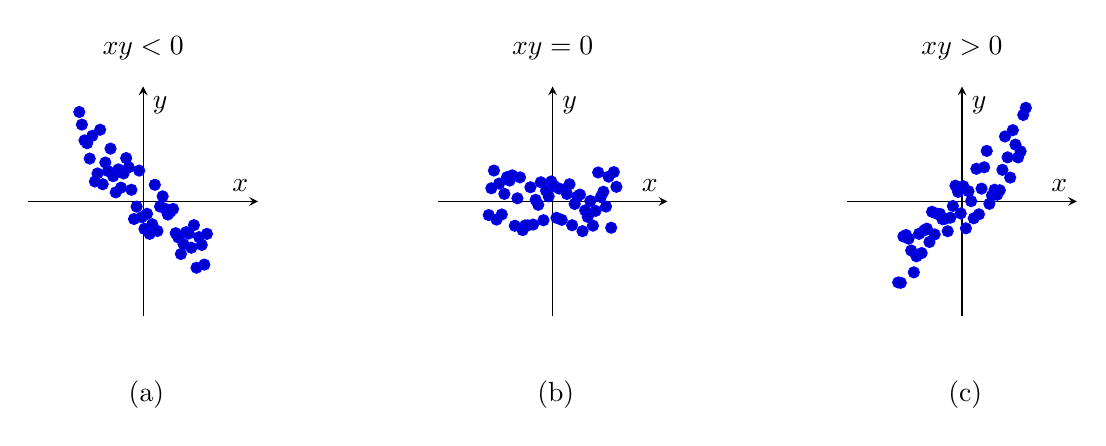
\begin{tikzpicture}
		% Negative covariance
		\begin{scope}[shift={(0,0)}]
			\begin{axis}[
				width=4.5cm, height=4.5cm,
				title={$\cov{x}{y} <0$},
				xlabel={$x$}, ylabel={$y$},
				xmin=-3, xmax=3, ymin=-3, ymax=3,
				xtick=\empty, ytick=\empty,
				axis lines=middle, enlargelimits
				]
				\addplot+[only marks, mark=*, samples=50, domain=-2:2] 
				({x}, {-x + rand});
			\end{axis}
			\node at (1.5,-1) {(a)};
		\end{scope}
		% Zero covariance
		\begin{scope}[shift={(5.2cm,0)}]
			\begin{axis}[
				width=4.5cm, height=4.5cm,
				title={$\cov{x}{y} =0$}, 
				xlabel={$x$}, ylabel={$y$},
				xmin=-3, xmax=3, ymin=-3, ymax=3,
				xtick=\empty, ytick=\empty,
				axis lines=middle, enlargelimits
				]
				\addplot+[only marks, mark=*, samples=50, domain=-2:2] 
				({x}, {rand});
			\end{axis}
			\node at (1.5,-1) {(b)};
		\end{scope}
		% Positive covariance
		\begin{scope}[shift={(10.4cm,0)}]
			\begin{axis}[
				width=4.5cm, height=4.5cm,
				title={$\cov{x}{y} > 0$},
				xlabel={$x$}, ylabel={$y$},
				xmin=-3, xmax=3, ymin=-3, ymax=3,
				xtick=\empty, ytick=\empty,
				axis lines=middle, enlargelimits
				]
				\addplot+[only marks, mark=*, samples=50, domain=-2:2] 
				({x}, {x + rand});
			\end{axis}
			\node at (1.5,-1) {(c)};
		\end{scope}
		\end{tikzpicture}
%			\caption{\Gls{scatterplot}s illustrating \gls{realization}s from three different \gls{probmodel}s for two 
%				\gls{rv}s with different covariance values. (a) Negative. (b) Zero. (c) Positive.}
%			\label{fig:covariance-examples_dict}
		\end{figure} 
		\foreignlanguage{greek}{Βλέπε επίσης:} \gls{rv}, \gls{probspace}, \gls{scatterplot}, \gls{realization}, \gls{probmodel}, \gls{expectation}. },
	first={covariance},
	text={covariance},
	user1={\foreignlanguage{greek}{συνδιακύμανση}}, %nominative
  	user2={\foreignlanguage{greek}{συνδιακύμανσης}} %genitive
}

\newglossaryentry{kroneckerproduct}
{name={Kronecker product}, 
	description={The Kronecker product \index{Kronecker product} of two matrices $\mA \in \mathbb{R}^{m \times n}$ 
		and $\mB \in \mathbb{R}^{p \times q}$ is a block matrix denoted $\mA \otimes \mB$ 
	 	and defined as \cite{GolubVanLoanBook}, \cite{HornMatAnalysis}
    		\[
      		\mA \otimes \mB =
      		\begin{bmatrix}
        		a_{11}\mB & \cdots & a_{1n}\mB \\
        		\vdots & \ddots & \vdots \\
        		a_{m1}\mB & \cdots & a_{mn}\mB
      		\end{bmatrix}
      		\in \mathbb{R}^{mp \times nq}.
    		\]
    		The Kronecker product is a special case of the tensor product for matrices and is 
		widely used in multivariate statistics, linear algebra, and structured \gls{ml} \gls{model}s. 
		It satisfies the identity $(\mA \otimes \mB)(\vx \otimes \vy) = (\mA\vx) \otimes (\mB\vy)$ 
		for vectors $\vx$ and $\vy$ of compatible dimensions. \\
		\foreignlanguage{greek}{Βλέπε επίσης:} \gls{ml}, \gls{model}. },
	first={Kronecker product},
	text={Kronecker product},
	user1={\foreignlanguage{greek}{γινόμενο} Kronecker} %nominative
}

\newglossaryentry{median}
{name={median},
	description={A\index{median} median $\med(x)$ of a real-valued \gls{rv} $x$ 
		is any number $m \in \mathbb{R}$ such that $\prob{ x \leq m} \geq 1/2$ and $\prob{ x \geq m} \geq 1/2$ \cite{LC}. 
 		\begin{figure}[H]
			\begin{center}
			\begin{tikzpicture}
  			\begin{axis}[
    			axis lines=middle,
    			xlabel={$m$},
    			ylabel={},
    			ymin=0, ymax=1.1,
    			xmin=-2, xmax=6,
    			xtick=\empty,
    			ytick={0,1/2,1},
    			domain=-2:6,
    			samples=200,
    			width=10cm,
    			height=6cm,
    			smooth,
    			enlargelimits=true,
    			clip=false
  			]
    			% Shifted sigmoid CDF
			\addplot[thick, blue, name path=cdf] {1/(1 + exp(-(x - 1)))} node[pos=0.5, above, yshift=15pt] {$\prob{x \leq m}$};    % Vertical and horizontal ruler at F(x) = 0.5
   			\draw[dashed, gray] (axis cs:1,0) -- (axis cs:1,0.5); % vertical
    			\draw[dashed, gray] (axis cs:-2,0.5) -- (axis cs:1,0.5); % horizontal
    			% Mark the median point
    			\filldraw[red] (axis cs:1,0.5) circle (2pt);
  			%  \node[below left] at (axis cs:1,0.5) {\footnotesize $(x{=}1,\ F(x){=}\tfrac{1}{2})$};
    			% Label next to curve
  			\end{axis}
			\end{tikzpicture} 
			\end{center}
 		\end{figure}  
 		We can define the median $\med(\dataset)$ 
 		of a \gls{dataset} $\dataset = \{ x^{(1)}, \ldots, x^{(\samplesize)} \in \mathbb{R} \}$ 
 		via a specific \gls{rv} $\tilde{x}$ that is naturally associated with $\dataset$. 
 		In particular, this \gls{rv} is constructed by $\tilde{x} = x^{(I)}$, with the index $I$ 
 		being chosen uniformly at random from the set $\{1,\ldots,\samplesize\}$, i.e., $\prob{I = \sampleidx}=1/\samplesize$ for 
 		all $\sampleidx=1,\ldots,\samplesize$. If the \gls{rv} $x$ is integrable, a median of $x$ 
 		is the solution of the following \gls{optproblem}: 
 		$$\min_{x' \in \mathbb{R}} \expect{|x - x'|}.$$ 
 		Like the \gls{mean}, the median of a \gls{dataset} $\dataset$ can also be used 
 		to estimate \gls{parameter}s of an underlying \gls{probmodel}. Compared 
 		to the \gls{mean}, the median is more robust to \gls{outlier}s. For example, 
 		a median of a \gls{dataset} $\dataset$ with more than one \gls{datapoint} does not 
 		change even if we arbitrarily increase the largest element of $\dataset$. In contrast, 
 		the \gls{mean} will increase arbitrarily.
		\begin{figure}[H]
		\centering
		\begin{tikzpicture}[scale=0.7, y=0.5cm, x=0.5cm]
			\begin{scope}
				\foreach \x/\y in {
					1/2, 4/3, 7/4
				} {
					\draw[dashed, gray] (\x, 0) -- (\x, \y);
					\filldraw[blue] (\x, \y) circle (2pt);
					\node[circle, inner sep=0pt] (ptA\x) at (\x, \y) {};
				}
				\draw[dashed, thick, darkgreen] (0.5, 3) -- (10.5, 3) node[right] {$\med(\dataset)$};
				\node at (7.5, -4) {(a)};
			\end{scope}
			\begin{scope}[xshift=12cm]
				\foreach \x/\y in {
					1/2, 4/3, 7/10
				} {
					\draw[dashed, gray] (\x, 0) -- (\x, \y);
					\filldraw[blue] (\x, \y) circle (2pt);
					\node[circle, inner sep=0pt] (ptB\x) at (\x, \y) {};
				}
				\draw[dashed, thick, darkgreen] (0.5, 3) -- (10.5, 3) node[right] {$\med\big(\widetilde{\dataset}\big)$};
				\node[above right=2pt and 2pt, red] at (ptB7) {outlier};
				\node at (7.5, -4) {(b)};
			\end{scope}
		\end{tikzpicture}
		\caption{The median is robust against \gls{outlier} contamination. (a) Original \gls{dataset} $\dataset$. (b) Noisy 
		\gls{dataset} $\widetilde{\dataset}$ including an \gls{outlier}. }
		\end{figure}
		\foreignlanguage{greek}{Βλέπε επίσης:} \gls{rv}, \gls{dataset}, \gls{optproblem}, \gls{mean}, \gls{parameter}, 
		\gls{probmodel}, \gls{outlier}, \gls{datapoint}, \gls{robustness}.}, 
	first={median}, 
	text={median} 
}

\newglossaryentry{characteristicfunc}
{name={characteristic function},
	description={The characteristic \gls{function}\index{characteristic function} 
		of a real-valued \gls{rv} $x$ is the \gls{function} \cite[Sec. 26]{BillingsleyProbMeasure}
		$$ \phi_{x}(t) \defeq \expect { \exp\,(j t x) } \mbox{ with } j = \sqrt{-1}.$$
		The characteristic \gls{function} uniquely determines the \gls{probdist} of $x$. \\
		\foreignlanguage{greek}{Βλέπε επίσης:} \gls{function}, \gls{rv}, \gls{probdist}.},
	first={characteristic function},
	text={characteristic function}
}

\newglossaryentry{matrix}
{name={\foreignlanguage{greek}{πίνακας}},
	description={A matrix\index{\foreignlanguage{greek}{πίνακας}} of size $\samplesize \times \nrfeatures$ is a two-dimensional array of numbers, 
% 		which is denoted  
%		$$
%  		\mA = \begin{bmatrix}
%   		A_{1,1} & A_{1,2} & \dots  & A_{1,\nrfeatures} \\
%		A_{2,1} & A_{2,2} & \dots  & A_{2,\nrfeatures} \\
%		\vdots  & \vdots  & \ddots & \vdots \\
%		A_{\samplesize,1} & A_{\samplesize,2} & \dots  & A_{\samplesize,\nrfeatures}
%		\end{bmatrix} \in \mathbb{R}^{\samplesize \times \nrfeatures}.
%		$$
%		Here, $A_{\sampleidx,\featureidx}$ denotes the matrix entry in the $\sampleidx$-th row and the 
%		$\featureidx$-th column. Matrices are useful representations of various mathematical objects \cite{StrangLinAlg2016}:
%		\begin{itemize}
%			\item Systems of linear equations: We can use a matrix to represent a system of linear equations 
%			$$ \begin{pmatrix}
%			A_{1,1} & A_{1,2} \\
%			A_{2,1} & A_{2,2}
%			\end{pmatrix}
%			\begin{pmatrix}
%				w_1 \\
%				w_2
%			\end{pmatrix}
%			=\begin{pmatrix}
%				y_1 \\
%				y_2
%			\end{pmatrix}
%			\quad \text{ compactly as } \quad \mA \vw = \vy.
%			$$
%    			One important example of systems of linear equations are the optimality condition for the 
%    			\gls{modelparams} within \gls{linreg}. 
%			\item \Gls{linearmap}s:
%			Consider a $\nrfeatures$-dimensional \gls{vectorspace} $\mathcal{U}$ and a $\samplesize$-dimensional \gls{vectorspace} $\mathcal{V}$. 
%			If we fix a basis $\mathbf{u}^{(1)},\ldots,\mathbf{u}^{(\nrfeatures)}$ for $\mathcal{U}$ and a basis $\mathbf{v}^{(1)},\ldots,\mathbf{v}^{(\samplesize)}$ 
%			for $\mathcal{V}$, each matrix $\mA \in \mathbb{R}^{\samplesize \times \nrfeatures}$ naturally defines a \gls{linearmap} $\alpha: \mathcal{U} \rightarrow \mathcal{V}$:
%   			$$\vu^{(\featureidx)} \mapsto \sum_{\sampleidx=1}^{\samplesize} A_{\sampleidx,\featureidx} \vv^{(\sampleidx)}.$$
%			\item \Gls{dataset}s: We can use a matrix to represent a \gls{dataset}. Each row 
%			corresponds to a single \gls{datapoint}, and each column corresponds to a specific 
%			\gls{feature} or \gls{label} of a \gls{datapoint}. 
%		\end{itemize}
%		\begin{figure}[H]
%		\begin{center}
%		\begin{tikzpicture}[x=2cm]
%			% LEFT: Standard basis vectors and unit square
%			\begin{scope}
%				\draw[->, thick] (0,0) -- (1,0) node[below] {$\vu^{(1)}$};
%				\draw[->, thick] (0,0) -- (0,1) node[above] {$\vu^{(2)}$};
%				%\draw[fill=gray!15] (0,0) -- (1,0) -- (1,1) -- (0,1) -- cycle;
%				%\node at (0.5,0.5) {\small unit square};
%				%\node at (0.5,-0.6) {standard basis};
%			\end{scope}
%			% RIGHT: Transformed basis vectors and parallelogram
%			\begin{scope}[shift={(3.2,0)}]
%				\draw[->, thick] (0,0) -- (1,0) node[below] {$\vv^{(1)}$};
%				\draw[->, thick] (0,0) -- (0,1) node[above] {$\vv^{(2)}$};
%				\coordinate (A) at (0.2,-1.0);
%				\coordinate (B) at (0.4,1.2);
%				\draw[->, very thick, red] (0,0) -- (A) node[below,right] {$\mA \vu^{(1)}\!=\!A_{1,1}\vv^{(1)}\!+\!A_{2,1}\vv^{(2)}$};
%				\draw[->, very thick, red] (0,0) -- (B) node[right,xshift=1pt] {$\mA \vu^{(2)}$};
%				%	\node[blue] at (0.25,1.25) {};
%				%	\node at (0.8,-0.6) {transformed basis};
%			\end{scope}
%			% Arrow between plots
%			\draw[->, thick] (1.6,0.5) to[bend left] node[midway, above] {$\mA$} (2.7,0.5);
%		%	\draw[->, thick] (1.3,0.5) -- (2.4,0.5) node[midway, above] {$\mA$};
%		\end{tikzpicture}
%		\end{center}
%		\caption{A matrix $\mA$ defines a \gls{linearmap} between two \gls{vectorspace}s.} 
%		\end{figure}
		\\
		\foreignlanguage{greek}{Βλέπε επίσης:} \gls{modelparams}, \gls{linreg}, \gls{linearmap}, \gls{vectorspace}, \gls{dataset}, 
		\gls{datapoint}, \gls{feature}, \gls{label}, \gls{linmodel}. },
	first={\foreignlanguage{greek}{πίνακας}},
	text={\foreignlanguage{greek}{πίνακας}},
	user1={\foreignlanguage{greek}{πίνακας}}, %nominative
	user2={\foreignlanguage{greek}{πίνακα}}, %genitive
	user3={\foreignlanguage{greek}{πίνακα}}, %accusative
	user4={\foreignlanguage{greek}{πίνακες}}, %nominativepl
	user5={\foreignlanguage{greek}{πινάκων}}, %genitivepl
	user6={\foreignlanguage{greek}{πίνακες}} %accusativepl
}

\newglossaryentry{vector}
{name={vector},
	description={A\index{vector} vector is an element of a \gls{vectorspace}. 
		In the context of \gls{ml}, a particularly important example of a \gls{vectorspace} 
		is the \gls{euclidspace} $\mathbb{R}^{\nrfeatures}$, where $\nrfeatures \in \mathbb{N}$ 
		is the (finite) dimension of the space. A vector $\vx \in \mathbb{R}^{\nrfeatures}$ 
		can be represented as a list or one-dimensional array of real numbers, i.e., 
		$x_1, \ldots, x_{\nrfeatures}$ with $x_\featureidx \in \mathbb{R}$ for 
		$\featureidx = 1, \ldots, \nrfeatures$. The value $x_\featureidx$ is the $\featureidx$-th 
		entry of the vector $\vx$. It can also be useful to view a vector $\vx \in \mathbb{R}^{\nrfeatures}$ 
		as a \gls{function} that maps each index $\featureidx \in \{1, \ldots, \nrfeatures\}$ 
		to a value $x_\featureidx \in \mathbb{R}$, i.e., $\vx: \featureidx \mapsto x_\featureidx$. 
		This perspective is particularly useful for the study of \gls{kernelmethod}s.
		\begin{figure}[H]
			% Left: Stem plot
			\begin{minipage}[c]{0.48\textwidth}
				\centering 
				2, -1, 3, 0, -2, 1
				\begin{minipage}{\textwidth}
				\vspace{5ex}
				\centering
				{\selectfont (a)}
				\end{minipage}
			\end{minipage}
			\hfill
			% Right: Column vector
			\begin{minipage}{0.48\textwidth}
			\centering
			\begin{tikzpicture}
			\begin{axis}[
    				width=6.5cm,
    				height=5cm,
    				title={},
    				xlabel={index $\featureidx$},
    				ylabel={$x_\featureidx$},
   		 		ymin=-3.5, ymax=3.5,
    				xmin=0.5, xmax=6.5,
   	 			xtick={1,2,3,4,5,6},
    				ytick={-3,-2,-1,0,1,2,3},
    				axis x line=bottom,        % <-- horizontal axis at y=0
    				axis y line=left,          % <-- vertical axis on the left
    				grid=both,
    				major grid style={dotted, gray!60},
    				enlargelimits=0.1
			]
			\addplot+[ycomb, thick, mark=*]
    			coordinates {
        				(1,2)
        				(2,-1)
       	 			(3,3)
        				(4,0)
        				(5,-2)
        				(6,1)
    			};
			\end{axis}
			\node at (2,-2.5) {(b)};
			\end{tikzpicture}
			\end{minipage}
			\caption{Two equivalent views of a vector $\vx= \big( 2, -1, 3, 0, -2, 1 \big)^{T} \in \mathbb{R}^{6}$.
			(a) As a numeric array. (b) As a map $\featureidx \mapsto x_\featureidx$.}
			\label{fig:vector-function-dual_dict}
		\end{figure}
		\foreignlanguage{greek}{Βλέπε επίσης:} \gls{vectorspace}, \gls{ml}, \gls{euclidspace}, \gls{function}, 
		\gls{kernelmethod}, \gls{map}, \gls{linearmap}.},
	first={vector},
	text={vector}
}




